%%%%%%%%%%%%%%%%%%%%%%%%%%%%%%%%%%%%%%%%%%%%%%%%%%%%%%%%%%%%%%%%%%%%%%%%%
%                                                                       %
% ustthesis_test.tex: A template file for usage with ustthesis.cls      %
%                                                                       %
%%%%%%%%%%%%%%%%%%%%%%%%%%%%%%%%%%%%%%%%%%%%%%%%%%%%%%%%%%%%%%%%%%%%%%%%%

\documentclass[a4paper]{ustthesis}
\usepackage[square,numbers]{natbib}
\usepackage[T1]{fontenc}
%\usepackage{algorithm}
%\usepackage{algorithmic}
\usepackage{longtable}
\usepackage{url}
\usepackage{multirow}
\usepackage{graphics}
\usepackage{graphicx}
\usepackage{amsmath}
\usepackage{cases}
\usepackage{colortbl}
\usepackage{xcolor}
\usepackage{times}
\usepackage{array}

\usepackage{color}
\usepackage{hyperref}
\hypersetup{
    colorlinks=true,
    linkcolor=black,
    filecolor=blue,      
    urlcolor=blue,
    citecolor=blue,
}

\usepackage{tocloft}
% \renewcommand{\cftfigindent}{0pt}
% \renewcommand{\cftfignumwidth}{2em}


\usepackage{pdflscape}
\DeclareMathOperator*{\argmax}{argmax}      % for argmax

\usepackage{lipsum}
\usepackage{amsfonts}
\usepackage{amsfonts,amssymb,amsmath,mathrsfs}
\usepackage{graphicx}
\usepackage{epstopdf}
%\usepackage{algorithmic}
\usepackage{bm}

\ifpdf
  \DeclareGraphicsExtensions{.eps,.pdf,.png,.jpg}
\else
  \DeclareGraphicsExtensions{.eps}
\fi

\usepackage{amssymb}
%% The amsmath package provides various useful equation environments. 
\usepackage{tikz}
\usetikzlibrary{3d}
\usetikzlibrary {decorations.pathreplacing}
\usepackage{mlmath}
\newcommand{\mrm}[1]{\mathrm{#1}} % redefine mathrm

\newcommand{\rev}[1]{\textcolor{blue}{#1}}

\def\b{\boldsymbol}
\def\bs{\bm{\sigma}}
\def\e{\epsilon}
\def\z{\zeta}
\def\Z{\mathbb{Z}}
\def\R{\mathbb{R}}
\def\E{\mathbb{E}}
\def\bbP{\mathbb{P}}
\def\bfP{\mathbf{P}}
\def\bfX{\mathbf{X}}
\def\cL{\mathcal{L}}
\def\cO{O}
\def\cH{\mathcal{H}}
\def\Ld{\Lambda}
\def\calk{\mathcal{K}}
\def\Ai{\mathrm{\AA}}
\DeclareMathOperator{\supp}{supp}
% \DeclareMathOperator{\dist}{dist}
\DeclareMathOperator{\var}{var}
\DeclareMathOperator{\tr}{tr}
\DeclareMathOperator{\loc}{loc}
\DeclareMathOperator{\kl}{KL}
\DeclareMathOperator{\erf}{erf}
\DeclareMathOperator{\erfc}{erfc}
\def\Image{\mathrm{Im}}

\usepackage{geometry}
\geometry{left=3.5cm,right=3.5cm,top=3cm,bottom=4cm}

\usepackage{colortbl}
\usepackage{xcolor}
% a new command rm to remove the content
\usepackage{soul}
\newcommand{\rem}[1] {{\color{red}{\st{#1}}}}
\usepackage{bm}
\newcommand\Wtilde{\stackrel{\sim}{\smash{\mathcal{W}}\rule{0pt}{1.1ex}}}

\usepackage{algorithm}
\usepackage{algorithmicx}
\usepackage{algpseudocode}

%% The amssymb package provides various useful mathematical symbols
%\usepackage{amssymb}
%\usepackage{pifont}
%\usepackage[nointegrals]{wasysym}
%\usepackage{amsfonts,amssymb,amsbsy,latexsym,amsmath,tabulary,graphicx,times,caption,fancyhdr}
%\usepackage[utf8]{inputenc}
%\usepackage{url,multirow,morefloats,floatflt,cancel,tfrupee}
%\usepackage{mathrsfs}
%\usepackage{graphicx}
\urlstyle{rm}
%macros from Aleks
\newcommand{\V}[1]{\boldsymbol{#1}} %# vector
\newcommand{\M}[1]{\boldsymbol{#1}} %# matrix
\newcommand{\Set}[1]{\mathbb{#1}} %# set
\renewcommand{\d}[1]{\delta#1} %# \d{t} for small increment
\newcommand{\T}[1]{\text{#1}}

\newcommand{\grad}{\M{\nabla}} %gradient
\newcommand{\av}[1]{\left\langle #1\right\rangle } %take average
\makeatletter
\newcommand{\Biggg}{\bBigg@{3.5}}

\newcommand{\dprime}{\prime\prime} % double prime
\global\long\def\i{\iota}
\renewcommand{\i}{\iota} %i for imaginary unit
%\renewcommand{\i}{\mathsf i} %i for imaginary unit
\newcommand{\follows}{\quad\Rightarrow\quad} %=>
%\usepackage{amsthm}
\newcommand{\eqd}{\overset{d}{=}} %=^d
\newcommand{\te}{\text}

\renewcommand{\d}[1]{\delta#1} %# \d{t} for small increment
%\global\long\def\i{\iota}
%\renewcommand{\i}{\iota} %i for imaginary unit
\renewcommand{\i}{\mathsf i} %i for imaginary unit
\newcommand{\spe}[1]{\mathscr{#1}}  %important quantities in mathscr font
\newcommand{\m}[1]{\mathrm{#1}}

% Add a serial/Oxford comma by default.
\newcommand{\creflastconjunction}{, and~}

\newtheorem{thm}{Theorem}[section] 
\newtheorem{lem}[thm]{Lemma} 
\newtheorem{rmk}[thm]{Remark}
\newtheorem{defination}[thm]{Definition} 
\newtheorem{prop}[thm]{Proposition}
\newtheorem{corollary}[thm]{Corollary}

% Used for creating new theorem and remark environments
% \newsiamremark{remark}{Remark}
% \newsiamremark{hypothesis}{Hypothesis}
% \crefname{hypothesis}{Hypothesis}{Hypotheses}
% \newsiamthm{claim}{Claim}

% \usepackage{latexsym}
    % Use the "latexsym" package when encountering the following error:
    %   ! LaTeX Error: Command \??? not provided in base LaTeX2e.
% \usepackage{epsf}
    % Use the "epsf" package for including EPS files.

%%%%%%%%%%%%%%%%%%%%%%%%%%%%%%%%%%%%%%%%%%%%%%%%%%%%%%%%%%%%%%%%%%%%%%%%%
%                                                                       %
% Preambles. DO NOT ERASE THEM. Change to suite your particular purpose.%
%                                                                       %
%%%%%%%%%%%%%%%%%%%%%%%%%%%%%%%%%%%%%%%%%%%%%%%%%%%%%%%%%%%%%%%%%%%%%%%%%

% \title{Fast Algorithms for Simulating Quasi-2D Coulomb Systems}  % Title of the thesis.
\title{Confined Quasi-2D Coulomb Systems: Theory, Algorithms, and Applications}
\author{GAO, Xuanzhao}     % Author of the thesis.
\degree{\PhD}             % Degree for which the thesis is. Options: \AM \MSc \MPhil \PhD
\stage{\Thesis}              % Stage of PhD document; use \Thesis for all other degree. Options: \PQE \Proposal \Thesis
\subject{IIP-AMAT} % Subject of the Degree.
\department{Academy of Interdisciplinary Studies (AIS)}       % Department to which the thesis is submitted.
\advisor{GAN, Zecheng}     % Supervisor. Additional co-supervisor can be added using \member
\member{XIANG, Yang, Thesis Supervisor}
\member{LIU, Jin-Guo, Thesis Supervisor}
%\acting      % Uncomment for Accting department head
\depthead{QU, Huamin}     % department head.
\defencedate{2025}{05}{27}     % \defencedate{year}{month}{day}.

% NOTE:
%   According to the sample shown in the guidelines, page number is
%   placed below the bottom margin.  However, if the author prefers
%   the page number to be printed above the bottom margin, please
%   activate the following command.

%\PNumberAboveBottomMargin

\begin{document}
%\begin{CJK}{UTF8}{song}  % Bitstream Cyber Bit song ti

%\begin{CJK*}{UTF8}{gbsn} % Arphic song ti

%%%%%%%%%%%%%%%%%%%%%%%%%%%%%%%%%%%%%%%%%%%%%%%%%%%%%%%%%%%%%%%%%%%%%%%%%
%                                                                       %
% Now the actual Thesis. The order of output MUST be followed:          %
%                                                                       %
%    1) TITLEPAGE                                                       %
%                                                                       %
% The \maketitle command generates the Title page as well as the        %
% Signature page.                                                       %
%                                                                       %
%%%%%%%%%%%%%%%%%%%%%%%%%%%%%%%%%%%%%%%%%%%%%%%%%%%%%%%%%%%%%%%%%%%%%%%%%

\maketitle

%%%%%%%%%%%%%%%%%%%%%%%%%%%%%%%%%%%%%%%%%%%%%%%%%%%%%%%%%%%%%%%%%%%%%%%%%
%                                                                       %
%     2) DEDICATION (Optional)                                          %
%                                                                       %
% The \dedication and \enddedication commands are optional. If          %
% specified it generates a page for dedication.                         %
%
%%%%%%%%%%%%%%%%%%%%%%%%%%%%%%%%%%%%%%%%%%%%%%%%%%%%%%%%%%%%%%%%%%%%%%%%%

% \dedication
% % This is an optional section.
% \noindent You raise me up, so I can stand on mountains;\\
you raise me up, to walk on stormy seas.\\
I am strong when I am on your shoulders.\\
You raise me up, to more than I can be. --- ``You raise me up'' lyrics by Brendan Graham.\\

\par \hfill To my mother, CHAN Siu-ngan (1958.12.21 - 2017.12.12).\\

\par ~\\

\par
\noindent 找一個夢 走一條路 \\
你像月光夜夜在祈禱我幸福 照亮我踏的每一步\\
我不會哭 我不會輸 \\
我在月光守護的黑夜裡\\
看著自己真的像你 走你走過的路 --- 《月光》 易家揚 詞\\

\par \hfill 致陳笑顏(1958.12.21 - 2017.12.12),我敬愛的媽媽

% \enddedication
% \newpage

%%%%%%%%%%%%%%%%%%%%%%%%%%%%%%%%%%%%%%%%%%%%%%%%%%%%%%%%%%%%%%%%%%%%%%%%%
%                                                                       %
%     3) ACKNOWLEDGMENTS                                                %
%                                                                       %
% \acknowledgments and \endacknowledgments defines the                  %
% Acknowledgments of the author of the Thesis.                          %
%                                                                       %
%%%%%%%%%%%%%%%%%%%%%%%%%%%%%%%%%%%%%%%%%%%%%%%%%%%%%%%%%%%%%%%%%%%%%%%%%

\acknowledgments
% acknowledgments

Completing this thesis is a long journey, and I would like to thank everyone who has helped me along the way.

First and foremost, I would like to express my deepest gratitude to my advisor, Prof. Zecheng Gan from Hong Kong University of Science and Technology (Guangzhou), under whose guidance the main work of this thesis was completed.
In the summer of 2021, I became Prof. Gan's first PhD student, marking the beginning of our journey together.
During my undergraduate studies, I majored in Applied Physics. 
Although I chose to enter this entirely new field due to my interest in applied mathematics and scientific computing, I had not received sufficient training in these areas.
However, Prof. Gan never dismissed me for my lack of knowledge. Instead, he patiently tutored me in the fundamentals of scientific computing and applied mathematics, and provided guidance and support whenever I encountered difficulties.
Under these circumstances, I was able to quickly begin our first project and make progress in my academic growth.
During my PhD study, I often felt inadequate: I wasn't particularly clever, having been just an average student during my undergraduate years; I wasn't meticulous enough, often making mistakes due to carelessness; and I wasn't always diligent, frequently being distracted.
Yet Prof. Gan never criticized me for my shortcomings. 
Instead, he consistently encouraged me, supported me, and helped me improve.
Prof. Gan also gave me considerable academic freedom, allowing me to explore different ideas and directions. 
It was through this exploration that I gradually found the direction I was willing to dedicate myself to, which has shaped who I am today.

Second, I would like to express my gratitude to several other professors who have provided invaluable guidance and support throughout my research journey. 
I am particularly thankful to Prof. Zhenli Xu from Shanghai Jiao Tong University. 
During my first semester of junior year, I had the privilege of being a visiting student in Prof. Xu's group.
Although one semester may seem brief, Prof. Xu's rigorous research approach and passion for science left a lasting impression on me. 
This period marked a significant transformation, as I evolved from a naive student into a researcher with a deep enthusiasm for scientific inquiry. Prof. Xu's comprehensive understanding of the field has been instrumental in guiding my future research direction.
I also deeply appreciate Prof. Jin-Guo Liu of Hong Kong University of Science and Technology (Guangzhou), my co-supervisor. 
Although our relationship did not begin as advisor and student, he generously shared his knowledge with me. His innovative research mindset and professional programming skills have been immensely beneficial. 
Collaborating with Prof. Liu on open-source projects and research work has been both educational and enjoyable. The coding work for this thesis would have been challenging to complete without his assistance.
I am grateful to Prof. Shidong Jiang from the Flatiron Institute, with whom I have had numerous discussions over the past year. 
Prof. Jiang's ability to address the core issues has significantly enhanced the quality of my work.
Additionally, I would like to thank Prof. Yang Xiang from Hong Kong University of Science and Technology, Prof. Pan Zhang from the Institute of Theoretical Physics, Chinese Academy of Sciences, and Prof. Feng Pan from Singapore University of Technology and Design. 
Their support has been crucial in overcoming various challenges during my thesis, enabling me to complete my doctoral research on schedule.

I would also like to thank my collaborators, including Jiuyang Liang from the Flatiron Institute, Qi Zhou from Shanghai Jiao Tong University, and Yijia Wang from the Institute of Theoretical Physics, Chinese Academy of Sciences. 
The time spent with them has always been enjoyable, and discussions with them have always brought me new knowledge and ideas. 
Most of my work has been completed in collaboration with them. 
Whether as collaborators or friends, they are impeccable. 
Now we are all ready to embark on our own paths, and I hope that in the future, we will all shine in our respective fields.
I also want to thank my friends, Zheng Yang, Tianhao Hu, Yanyu Duan, Yusheng Zhao, Zhongyi Ni, and Hongchao Li. 
Without their companionship, the life of a PhD student would have been more difficult.

Finally, I would like to thank my parents for their unwavering support and encouragement.
Over the past four years, our family has faced many challenges, but they have shouldered all the burdens alone, just to keep me from being distracted.
Their unconditional support and love are the driving forces behind my progress.

This is indeed a long journey, but it is also only the beginning of my life as a scientist.
Knowledge begins with the recognition of one's ignorance. 
The realization that the search for knowledge is unending.
More challenges await me, and I will continue to explore the world with curiosity and passion, carrying forward the spirit of scientific inquiry.


\section*{A note of publications}

Most of the material in this thesis has already appeared in the following peer-reviewed publications or articles under review:
\begin{itemize}
    \item[A.] \textbf{Xuanzhao Gao}, Qi Zhou, Zecheng Gan, Jiuyang Liang; Accurate error estimates and optimal parameter selection in Ewald summation for dielectrically confined Coulomb systems. ArXiv: 2503.18126.
    \item[B.] Zecheng Gan, \textbf{Xuanzhao Gao}, Jiuyang Liang, Zhenli Xu; Random batch Ewald method for dielectrically confined Coulomb systems. Accepted by \emph{SIAM Journal on Scientific Computing}. ArXiv: 2405.06333.
    \item[C.] Zecheng Gan, \textbf{Xuanzhao Gao}, Jiuyang Liang, Zhenli Xu; Fast algorithm for quasi-2D Coulomb systems. \emph{Journal of Computational Physics}, 524: 113733, 2025.
    \item[D.] \textbf{Xuanzhao Gao}, Zecheng Gan; Broken symmetries in quasi-2D charged systems via negative dielectric confinement. \emph{The Journal of Chemical Physics}, 161 (1): 011102, 2024.
\end{itemize}
We also present some new material in this thesis, which will appear in a forthcoming publication:
\begin{itemize}
    \item[E.] \textbf{Xuanzhao Gao}, Zecheng Gan, Yuqing Li; Efficient particle-based simulations of Coulomb systems under dielectric nanoconfinement.
\end{itemize}
In particular, the material of Chapter~\ref{chp_icmewald2d} comes from A, where we present our theoretical analysis of the Ewald splitting method for confined quasi-2D Coulomb systems.
Then in Chapters~\ref{chp_soewald2d},~\ref{chp_rbe2d}, and~\ref{chp_quasiewald}, we present our fast algorithms for quasi-2D Coulomb systems, which are contributions from B, C, and E, respectively.
In Chapter~\ref{chp_applications}, we present results on numerical experiments on confined quasi-2D Coulomb systems from B and D.
\endacknowledgments
\newpage

%%%%%%%%%%%%%%%%%%%%%%%%%%%%%%%%%%%%%%%%%%%%%%%%%%%%%%%%%%%%%%%%%%%%%%%%%
%                                                                       %
%     4) TABLE OF CONTENTS                                              %
%                                                                       %
%%%%%%%%%%%%%%%%%%%%%%%%%%%%%%%%%%%%%%%%%%%%%%%%%%%%%%%%%%%%%%%%%%%%%%%%%

\tableofcontents

%%%%%%%%%%%%%%%%%%%%%%%%%%%%%%%%%%%%%%%%%%%%%%%%%%%%%%%%%%%%%%%%%%%%%%%%%
%                                                                       %
%     5) LIST OF FIGURES (If Any)                                       %
%                                                                       %
%%%%%%%%%%%%%%%%%%%%%%%%%%%%%%%%%%%%%%%%%%%%%%%%%%%%%%%%%%%%%%%%%%%%%%%%%

\newpage
\addcontentsline{toc}{chapter}{List of Figures}
\listoffigures

%%%%%%%%%%%%%%%%%%%%%%%%%%%%%%%%%%%%%%%%%%%%%%%%%%%%%%%%%%%%%%%%%%%%%%%%%
%                                                                       %
%     6) LIST OF TABLES (If Any)
%                                                                       %
%%%%%%%%%%%%%%%%%%%%%%%%%%%%%%%%%%%%%%%%%%%%%%%%%%%%%%%%%%%%%%%%%%%%%%%%%

\newpage
\addcontentsline{toc}{chapter}{List of Tables}
\listoftables

%%%%%%%%%%%%%%%%%%%%%%%%%%%%%%%%%%%%%%%%%%%%%%%%%%%%%%%%%%%%%%%%%%%%%%%%%
%                                                                       %
%     7) ABSTRACT                                                       %
%                                                                       %
% \abstract and \endabstract are used to define a short Abstract for    %
% the Thesis.                                                           %
%                                                                       %
%%%%%%%%%%%%%%%%%%%%%%%%%%%%%%%%%%%%%%%%%%%%%%%%%%%%%%%%%%%%%%%%%%%%%%%%%


%%%%%%%%%%%%%%%%%%%%%%%%%%%%%%%%%%%%%%%%%%%%%%%%%%%%%%%%%%%%%%%%%%%%%%%%%
%                                                                       %
%     8) The Actual Contents                                            %
%                                                                       %
% The command \chapters MUST BE USED to ensure that the entire content  %
% of the Thesis is double-spaced (in version 1.0).                      %
%                                                                       %
% However, in version 2.0, \chapters will be automatically added in     %
% the beginning of the first chapter.                                   %
%                                                                       %
%%%%%%%%%%%%%%%%%%%%%%%%%%%%%%%%%%%%%%%%%%%%%%%%%%%%%%%%%%%%%%%%%%%%%%%%%

%%\chapters         % Not necessary with ustthesis.cls (v2.0).

%%%%%%%%%%%%%%%%%%%%%%%%%%%%%%%%%%%%%%%%%%%%%%%%%%%%%%%%%%%%%%%%%%%%%%%%%
%                                                                       %
% Each chapter is defined via the \chapter command. The usual sectional %
% commands of LaTeX are also available.                                 %
%                                                                       %
%%%%%%%%%%%%%%%%%%%%%%%%%%%%%%%%%%%%%%%%%%%%%%%%%%%%%%%%%%%%%%%%%%%%%%%%%

\chapter{Introduction}
\label{chp_intro}
\section{Background}

Confined quasi two-dimensional (quasi-2D) Coulomb systems~\cite{mazars2011long}, which are macroscopic in two dimensions but with atomic-size thickness in the other, have caught much attention in studies of magnetic and liquid crystal films, supercapacitors, crystal phase transitions, dusty plasmas, ion channels, superconductive materials, and quantum devices~\cite{kawamoto2002history, hille2001ionic, teng2003microscopic, Messina2017PRL, mazars2011long, saito2016highly, liu20192d}. 
Typically, such systems possess a nano-sized longitudinal thickness in the $z$ direction, achieved through confinement, bulk-like and modeled as periodic in the transverse $xy$ directions, hence endowed with an inherent multi-scale nature.
Due to the confinement effect, such systems can exhibit various interesting behaviors for future nanotechnologies; prototype examples include graphene~\cite{novoselov2004electric}, metal dichalcogenide monolayers~\cite{kumar2012tunable}, and colloidal monolayers~\cite{mangold2003phase}.

Among quasi-2D systems, charged particles confined by materials with different dielectric constants are of particular interest. 
The so-called \emph{dielectric confinement effect} can further lead to inhomogeneous screening, compared to bulk systems, or even broken symmetries near interfaces~\cite{C0NR00698J,wang2016inhomogeneous,gao2024broken}.
These effects are crucial in a wide range of applications, including the behavior of water, electrolytes, and ionic liquids confined within thin films~\cite{raviv2001fluidity}, ion transport in nanochannels~\cite{zhu2019ion}, and self-assembly of colloidal and polymer monolayers~\cite{kim2017imaging}.
In these systems, substrate materials used for nanoscale confinement can range from dielectric to metallic, and nowadays electromagnetic metamaterials, which have been developed with permittivities that can take negative values~\cite{veselago1967electrodynamics, smith2004metamaterials, cheng2017tunable, xie2022recent, xu2020polyaniline} when excited by electromagnetic waves of specific frequencies.  
It should be noted that materials with \emph{negative static permittivity} have drawn considerable attention, although rarely seen, their existence has been predicted in materials such as metals and nonideal plasma~\cite{Dolgov1918admissible,homes2001optical}. More recently, it has been experimentally achieved in a wide range of materials such as VO$_2$ films~\cite{kana2016thermally}, graphene~\cite{nazarov2015negative}, nanocolloids~\cite{shulman2007plasmalike}, and polymeric systems~\cite{yan2013negative}.
Interestingly, even for water, the perpendicular component of its tensorial dielectric function has been observed to be negative within sub-Angstrom distances from the surface by nano confinement~\cite{Kornyshev1996Static, Schlaich2016Water, Kornyshev2021Nonlocal}.


% To study the behavior of quasi-2D Coulomb systems, molecular dynamics (MD) simulations is one of the most powerful tools.
% By tracking the positions and velocities of all particles, MD can provide a detailed description of the system's static and dynamic properties.
% In MD simulations, the system is modeled as a collection of particles, which interact with each other through potential functions and the time evolution of the system is determined by the Newton's laws of motion.
% Thus, time cost of MD simulations is dominated by the calculation of the derivatives of the potential energy with respect to the particle positions, i.e. the force between particles.
% For the short-range potential such as the Lennard-Jones potential, the computational cost scales as $O(N)$ with the number of particles $N$ based on the neighbor list algorithm and the real space truncation.
% For long-range interactions such as the Coulomb interaction, the potential energy can be generally expressed as the lattice kernel summations in the form of

For numerical simulation of quasi-2D Coulomb systems, it is of great importance to evaluate lattice kernel summations in the form of
\begin{equation}\label{eq::phi12}
	\phi(\V x) = \sum_{\V{m}} \sum_{j = 1}^{N} \rho_j K(\V{x} - \V{y}_j + \V{m} \circ \V{L})\;,
\end{equation}
where~$\V{x}, \V{y}_j \in \mathbb{R}^3$ are $3$-dimensional vectors in a rectangular box $\Omega$ with $\V{L}$ the vector of its edge lengths, $\rho_j$ refers to the density or weight, $\V{m} \in \mathbb{Z}^2 \otimes \{0\}$ exerts periodicity in the first $2$ directions, ``$\circ$'' represents the Hadamard product, and~$K(\V{x})$ is the kernel function whose form depends on the interested physical problem. 
For homogeneous systems without dielectric confinements, the kernel function is given by $K(\V{x}) = \abs{\V{x}}^{-1}$.
For such long-range interactions, the computational cost scales as $O(N^2)$ in the naive pair-wise implementation, which greatly limits the size of the system that can be studied.


For fully-periodic or free-space Coulomb systems, various fast algorithms have been developed to reduce the computational cost, such as the fast multipole methods (FMM)~\cite{greengard1987fast,cheng1999fast,ying2004kernel}, fast Fourier transform (FFT) based Ewald-splitting methods~\cite{hockney2021computer,darden1993particle,essmann1995smooth} and the recently proposed random batch Ewald (RBE) method~\cite{jin2021random, liang2022superscalability,liang2024JCP}.
These fast algorithms have been successfully applied to large-scale simulations of Coulomb systems in various ensembles and have reached the complexity of $O(N\log N)$ or even $O(N)$.
 
For quasi-2D systems,  numerous methods have also been developed over the past decades, mostly relyinging on modifications to the FMM and FFT-based Ewald methods to achieve $O(N\log N)$ or even $O(N)$ complexity.
One important work is the Ewald2D method~\cite{parry1975electrostatic}, which directly applies the Ewald-splitting technique for quasi-2D systems, it scales as $O(N^2)$ and is found to be slowly convergent due to the oscillatory nature of the Green's function for quasi-2D geometry.
To further accelerate the convergence of the quasi-2D lattice summation, more methods have been proposed, including the MMM2D method~\cite{arnold2002mmm2d}, the periodic FMM method~\cite{yan2018flexibly}, and the spectral Ewald method~\cite{lindbo2012fast}.
Instead of exactly solving the quasi-2D problem, alternative approaches are to approximate the quasi-2D summations by 3D periodic summations with correction terms, such as the Yeh--Berkowitz (YB) correction~\cite{yeh1999ewald} and the electric layer correction (ELC)~\cite{arnold2002electrostatics}.
These correction methods effectively reduce the computational cost and are simple to implement, but lack control of accuracy.

The methods mentioned above encounter challenges when addressing sharp dielectric interfaces. In recent years, various strategies have been developed to effectively simulate quasi-2D systems under dielectric confinements.
\rev{Servial approaches have been developed to effectively simulate quasi-2D systems under dielectric confinements.}
A common approach is by combining the image charge method (ICM)~\cite{jackson1999classical,frenkel2023understanding}, where the polarization effects induced by dielectric planar interfaces are modeled through an infinite series of reflected image charges in homogeneous space.
Specifically, this approach truncates the infinitely reflected image charge series along the $z$-direction to a finite number of reflection layers. 
This reduction transforms the original dielectrically inhomogeneous system into a homogeneous one, albeit with an expanded dimension in $z$.
The remaining computational tasks can be effectively handled using the Ewald2D summation method~\cite{parry1975electrostatic,zhonghanhu2014JCTC}. While conceptually straightforward, this ICM-Ewald2D approach is computationally inefficient due to its $O(N^2)$ complexity.
\rev{
	Another approach is the boundary element method (BEM)~\cite{barros2014efficient,nguyen2019incorporating}, which solves the potential on the boundary of the system and then extends it to the interior using the Green's function. 
	This approach is very flexiable and can be applied to various geometries, but it is computationally expensive due to the need to solve a large linear system.
}
Several alternative approaches have been developed over recent years, including the fast Fourier-Chebyshev spectral method~\cite{maxian2021fast,gao2024fast}, and the harmonic surface mapping method~\cite{liang2020harmonic,liang2022hsma}.
When combined with the fast multipole method (FMM)~\cite{greengard1987fast,kohnke2020gpu}, or the fast Fourier-Chebyshev transform~\cite{trefethen2000spectral}, these methods can achieve computational complexities of $ O(N\log N)$ or even $ O(N)$.

Among existing approaches, a widely adopted technique involves reformulating the exact Ewald2D summation in terms of 3D Ewald summation, effectively approximating the quasi-2D problem with a fully periodic one.
Then, to eliminate unwanted contributions from periodic replicas along the $z$-axis, correction terms such as the Yeh-Berkowitz (YB) correction~\cite{yeh1999ewald,dos2015electrolytes} and the electric layer correction (ELC)~\cite{arnold2002electrostatics,tyagi2008electrostatic} have been introduced.
Its advantages include: (a) the use of 3D fast Fourier transform (FFT) to achieve $ O(N\log N)$ computational complexity~\cite{yuan2021particle,huang2024pmc}; 
(b) the straightforward incorporation of polarization contributions via image charges, as demonstrated in methods such as ICM-ELC~\cite{tyagi2008electrostatic}, ICM-Ewald3D~\cite{dos2015electrolytes}, and ICM-PPPM~\cite{yuan2021particle}; 
and (c) the minimal modifications needed to integrate these quasi-2D electrostatic solvers into mainstream software~\cite{ABRAHAM201519,thompson2021lammps}, where 3D periodic solvers have been extensively optimized.

% These approaches address the polarization effect either by introducing image charges for slab interfaces, effectively transforming the system into a homogeneous one (albeit with a considerable increase in thickness along the $z$-direction)~\cite{tyagi2007icmmm2d,tyagi2008electrostatic,dos2015electrolytes,yuan2021particle,liang2020harmonic}, or by numerically solving the Poisson equation with interface conditions~\cite{maxian2021fast, nguyen2019incorporating, ma2021modified}. 
% They all rely on either FMM or FFT to achieve $O(N)$ or $O(N\log N)$ complexity, respectively;

% We will not delve into a comprehensive review and comparison of these methods; instead, we will highlight two crucial aspects: 1) they all rely on either FMM or FFT to achieve   {$O(N)$ or $O(N\log N)$ complexity, respectively;} and 2) the computational cost significantly increases compared to the homogeneous case, especially for \emph{strongly confined} systems (i.e., with a large aspect ratio of simulation box). 
% In this scenario, FFT-based methods require a significant increase in   {resolution} to accommodate for the extended system thickness (i.e. zero-padding), while FMM-based methods require incorporating more near-field contributions and solving a possibly ill-conditioned linear system~\cite{pei2023fast}.

% However, different from the fully-periodic or free-space systems, quasi-2D systems possess a reduced symmetry, which gives rise to new phenomena, but also brings formidable challenges in both theory and computation.
% The first challenge comes from the involved \emph{long-range} interaction kernels, including but not limited to Coulomb and dipolar kernels in electrostatics, Oseen and Rotne-Prager-Yamakawa kernels in hydrodynamics and the static exchange-correlation kernels in density functional theory calculations. 
% The anisotropy of such systems poses extra challenges for simulations:
% (1) the periodic and non-periodic directions need to be handled separately due to their different boundary conditions and length scales;
% (2) the convergence properties of the lattice kernel summation requires careful consideration, which largely depend on the well-poseness of the underlying PDEs. 
% Another challenge comes from practical applications.
% To accurately determine the phase diagram of a many-body system may require thousands of simulation runs under different conditions~\cite{levin2002electrostatic}, each with billions of time steps to sample ensemble averages.
% Moreover, to eliminate the finite size effect, millions of free particles need to be simulated. Such large-scale simulations are especially required for quasi-2D systems, so as to accommodate its strong anisotropy, and resolving possible boundary layers forming near the confinement surfaces~\cite{mazars2011long}. 
% The cumulative impact of these considerations poses significant challenges for numerical simulations for quasi-2D systems. 

% To address these issues associated with the particle-based simulation of quasi-2D systems, a variety of numerical methods have been developed.
% Most of them also fall into two categories: 
% (1) Fourier spectral methods~\cite{lindbo2012fast,nestler2015fast,doi:10.1021/acs.jctc.3c01124, maxian2021fast}, where particles are first smeared onto grids, and subsequently the underlying PDE is solved in Fourier domain where fast Fourier transform (FFT) can be used for acceleration; 
% (2) adaptive tree-based methods, where fast multipole method (FMM)~\cite{greengard1987fast} or tree code~\cite{Barnes1986Nature} orginally proposed for free-space systems can be extended to quasi-2D systems by careful extension to match the partially-periodic boundary conditions~\cite{yan2018flexibly,liang2020harmonic}. 
% Alternative methods have also been proposed, such as the Lekner summation-based MMM2D method~\cite{arnold2002novel}, multilevel summation methods~\cite{doi:10.1021/ct5009075,greengard2023dual}, and correction-based approaches such as Ewald3DC~\cite{yeh1999ewald} and EwaldELC~\cite{arnold2002electrostatics}, which first solve a fully-periodic system and then add the partially-periodic correction terms. 
% By combining with either FFT or FMM, these methods achieve $O(N\log N)$ or even $O(N)$ complexity. 

However, the issue of large-scale simulation of quasi-2D systems is still far from settled.
A few challenges remains. First, FFT-based methods need extra techniques to properly handle the non-periodic direction, such as truncation~\cite{parry1975electrostatic}, regularization~\cite{nestler2015fast}, or periodic extension~\cite{lindbo2012fast}, which may lead to algebraic convergence or require extra zero-padding to guarantee accuracy. 
Recent advancements by Shamshirgar \emph{et al.}~\cite{shamshirgar2021fast}, combining spectral solvers with kernel truncation methods (TKM)~\cite{vico2016fast}, have reduced the zero-padding factor from $6$ to $2$~\cite{lindbo2012fast}, which still requires doubling the number of grids with zero-padding. 
% A similar reduction is also reported in the work of Maxian \emph{et al. }\cite{maxian2021fast}. 
Second, the periodization of FMM needs to encompass more near-field contributions from surrounding cells~\cite{yan2018flexibly,barnett2018unified}. The recently proposed 2D-periodic FMM~\cite{pei2023fast} may offer a promising avenue; however, it has not yet been extended to partially-periodic problems.
Finally, it is worth noting that most of the aforementioned issues will become more serious when the aspect ratio of the simulation box is large, in which case the Ewald series summation will converge much slower~\cite{arnold2002electrostatics}, and the zero-padding issue of FFT-based methods also becomes worse~\cite{maxian2021fast}.
Thus, efficient and accurate simulation of quasi-2D systems is still an open problem and a great challenge, especially for systems with large aspect ratios and strongly polarizable interfaces.


In this thesis, we focus on the study of confined quasi-2D Coulomb systems, including theoretical analysis, algorithm development and applications.
We provide comprehensive theoretical analysis including rigorous error estimates and complexity bounds, which are thoroughly validated through extensive numerical experiments.
We introduce a novel class of fast summation methods for quasi-2D Coulomb systems that synergistically combines the Ewald splitting technique with random batch sampling. 
Our proposed methods achieve optimal $O(N)$ computational complexity while maintaining high efficiency for strongly confined quasi-2D systems, even in challenging scenarios involving large aspect ratios and sharp dielectric interfaces. 
We also show a few applications of our methods to the simulation of quasi-2D Coulomb systems, including the study of broken symmetry in quasi-2D Coulomb systems and the simulation of electrolytes confined by dielectric interfaces.

\section{Thesis outlines}

The content of this thesis can be roughly divided into three parts, which are summarized as follows.

The first part focuses on the theoretical analysis about long-range interactions in quasi-2D Coulomb systems.

In Chapter~\ref{chp_preliminaries}, we introduce the physical model and mathematical notations for dielectric confined quasi-2D Coulomb systems.
Then we revisit the Ewald summation methods for both triply-periodic and doubly-periodic Coulomb systems.
We also provide a brief introduction to the random batch sampling method for fully-periodic Coulomb systems.

In Chapter~\ref{chp_icmewald2d}, we first introduce the Ewald summation method for dielectrically confined quasi-2D Coulomb systems, focusing on the ICM-Ewald2D method and its reformulation.
Then we provide detailed error analysis and guidelines for optimal parameter selection in these methods, along with extensive numerical validation of their performance for dielectrically confined quasi-2D systems.

In the second part, we introduce a novel class of fast summation methods for quasi-2D Coulomb systems.

In Chapter~\ref{chp_soewald2d}, we first introduce the kernel approximation technique called the sum-of-exponential (SOE) approximation, which approximates an arbitrary kernel function by a linear combination of exponential functions.
Then, based on the SOE approximation, we propose an algorithm named the sum-of-exponential Ewald2D (SOEwald2D) method, which utilizes the SOE approximation and the random batch sampling method to accelerate the Ewald2D summation for quasi-2D Coulomb systems without dielectric confinements.
Numerical results are provided to validate the accuracy and efficiency of the proposed method.

In Chapter~\ref{chp_rbe2d}, we focus on the quasi-2D Coulomb systems with dielectric confinements.
We first provide a rigorous error analysis for the combination of the image charge method and the Ewald summation formula.
Then, we introduce a novel algorithm called the random batch Ewald2D (RBE2D) method, which efficiently handles quasi-2D Coulomb systems with dielectric confinements while maintaining excellent scalability for large-scale simulations on modern supercomputing architectures.
Detailed numerical results are provided to validate the accuracy and efficiency of the proposed method.

In Chapter~\ref{chp_quasiewald}, we investigate quasi-2D systems with negative dielectric confinements, where the polarizable materials possess negative dielectric constants, which results in failure of ICM-based methods.
% The previous methods based on the image charge method break down in such systems due to the unusual polarization effects.
To overcome the numerical challenges, we develop the quasi-Ewald method (QEM), which introduces a novel quasi-Ewald splitting technique.
We show that with proper singularity subtraction, the QEM can be extended to handle negative dielectric confinements.
Numerical results are also provided for validation.
% Using this method, we explore the behavior of negatively confined quasi-2D charged systems and discover remarkable spontaneous symmetry breaking (SSB) phenomena emerging in symmetrically charged binary particle systems.

In the third part (Chapter~\ref{chp_applications}), we demonstrate practical applications of our methods through two key studies of quasi-2D Coulomb systems. 
First, we conduct all-atom molecular dynamics simulations of the SPC/E water model under both standard and dielectrically confined conditions. 
These simulations validate the efficiency, accuracy, and scalability of our methods for large-scale real-world applications. 
Second, we investigate negatively confined electrolytes, revealing a fascinating spontaneous symmetry breaking (SSB) phenomenon that emerges in symmetrically charged binary particle systems purely through confinement effects.

Finally, Chapter~\ref{chp_conclusion} concludes this thesis with a comprehensive summary of our methodological contributions. 
We critically evaluate the strengths and limitations of our proposed algorithms and outline promising future research directions for both theoretical developments and practical applications in computational physics and materials science.
\newpage

\chapter{Preliminaries}
\label{chp_preliminaries}
This chapter introduces the fundamental concepts and mathematical framework underlying this thesis.
We begin by presenting confined quasi-2D Coulomb systems and establishing the mathematical notation used throughout.
We then provide a comprehensive review of Ewald summation methods, focusing on the Ewald splitting technique and its applications to both fully and doubly periodic systems.
The chapter concludes with an overview of the random batch Ewald (RBE) method, an efficient approach for accelerating electrostatic energy computations in fully periodic systems.

\section{Confined quasi-2D Coulomb systems}

Confined quasi-2D Coulomb systems are three-dimensional models characterized by double periodicity in the $xy$ dimensions and confinement by planar dielectric interfaces along the $z$-axis.
The characteristic length scale in the non-periodic direction is often significantly smaller than that in the periodic directions. 
In what follows, we present the mathematical formulation of the model.

Consider two parallel dielectric interfaces positioned at $z=0$ and $z=H$, dividing the entire 3D space $\mathbb{R}^3$ into three distinct layers. 
From top to bottom, these layers are denoted as $\Omega_{\text{u}}$, $\Omega_{\text{c}}$ and $\Omega_{\text{d}}$, respectively. 
The central simulation cell $\Omega\in\Omega_{\text{c}}$ has side lengths~$\bm{L}=(L_x, L_y, H)$ and contains $N$ particles located at $\{\V{r}_i\}_{i=1}^{N}$ with charges $\{q_i\}_{i=1}^{N}$. 
The total charge neutrality condition is assumed, i.e., $\sum_{i=1}^{N}q_i=0$. The dielectric permittivity is a piecewise constant function, defined as:
\begin{equation}\label{eq:sanwich}
    \eps(\V{r})=\left\{
        \begin{array}{ll}
        \epsilon_{\mrm{u}}, &\, {\V{r} \in \Omega_{\mrm{u}}},\\
        \epsilon_{\mrm{c}}, &\, {\V{r} \in \Omega_{\mrm{c}}},\\
        \epsilon_{\mrm{d}}, & \,{\V{r} \in \Omega_{\mrm{d}}},
    \end{array} \right.
\end{equation}
where~$\eps_{\T u}$,~$\eps_{\T c}$ and~$\eps_{\T d}$ are all positive constants, whose specific values depend on materials properties inside each layer. 
Without loss of generality, we set~$\eps_{\T c} = 1$ in this thesis if not specified.
An illustration of the quasi-2D charged system is shown in Fig.~\ref{fig:box}.

\begin{figure}[htbp]
    \centering
    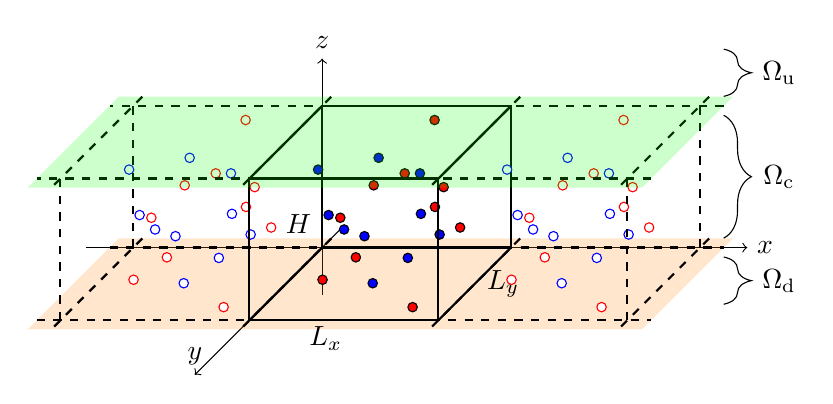
\begin{tikzpicture}[scale=0.6]

        \draw[->] (-5, 0, 0) -- (9, 0, 0) node[right] {$x$}; % x-axis
        \draw[->] (0, -1, 0) -- (0, 4, 0) node[above] {$z$}; % y-axis
        \draw[->] (0, 0, -1) -- (0, 0, 7) node[above] {$y$}; % z-axis

        \fill[orange, opacity=0.2] (-4.5, 0, -0.5) -- (8.5, 0, -0.5) -- (8.5, 0, 4.5) -- (-4.5, 0, 4.5);
        % \fill[orange, opacity=0.2] (-4.5, 0, 4.5) -- (8.5, 0, 4.5) -- (8.5, -0.5, 4.5) -- (-4.5, -0.5, 4.5);
        % \fill[orange, opacity=0.2] (8.5, 0, -0.5) -- (8.5, 0, 4.5) -- (8.5, -0.5, 4.5) -- (8.5, -0.5, -0.5);

        \draw[thick] (0, 0, 0) -- (4, 0, 0) -- (4, 3, 0) -- (0, 3, 0) -- cycle; % Bottom face

        \foreach \x/\y/\z in {1.1681915835663497/0.4784386449304706/3.0114784670813646, 1.37700874310584/0.4564910752408716/1.723302872827872, 3.730994750135867/1.2345031904085388/2.103105645365449, 1.827895374334192/2.07357017874381/3.746941345635766, 3.066558538444058/1.5385426337573604/1.7619877149348904, 1.323901301301564/1.5495075401772844/0.6031052215686215, 3.756938726146066/2.4640736386255653/3.077635065930065, 2.8772957887165047/2.6997418470234025/2.9329762207627343, 3.2340462748359378/0.05840416805411408/3.426026606528974, 2.6025039709080175/2.9218252913656833/0.57717965442315666} {
            \draw[fill=red] (\x, \y, \z) circle (0.1);
        }

        \foreach \x/\y/\z in {2.6498617350978773/2.150049613814989/1.5048602780413822, 3.089169032276023/1.0562600341829351/3.3127362964215057, 2.5980246280095605/0.7722521776014004/3.9662770148938087, 1.1349256153410514/2.870534190907561/3.169316637530182, 3.1201708293697656/0.9091412698002154/1.6441954803083996, 1.9206578784987878/2.6240285163641914/1.8820001242058, 2.21640094284661/0.839090054913301/0.3248449650128413, 1.7055625414319642/1.0502926700849304/2.1025386222981464, 1.9224549177172139/1.8402480747416887/3.7853267350243893, 0.6942437596034523/1.2454445897320752/1.4473021778716602} {
            \draw[fill=blue] (\x, \y, \z) circle (0.1);
        }

        \foreach \dx/\dy in {-4/0, 4/0} {
            \foreach \x/\y/\z in {1.1681915835663497/0.4784386449304706/3.0114784670813646, 1.37700874310584/0.4564910752408716/1.723302872827872, 3.730994750135867/1.2345031904085388/2.103105645365449, 1.827895374334192/2.07357017874381/3.746941345635766, 3.066558538444058/1.5385426337573604/1.7619877149348904, 1.323901301301564/1.5495075401772844/0.6031052215686215, 3.756938726146066/2.4640736386255653/3.077635065930065, 2.8772957887165047/2.6997418470234025/2.9329762207627343, 3.2340462748359378/0.05840416805411408/3.426026606528974, 2.6025039709080175/2.9218252913656833/0.57717965442315666} {
            \draw[draw=red, fill=white] (\x + \dx, \y + \dy, \z) circle (0.1);
        }

            \foreach \x/\y/\z in {2.6498617350978773/2.150049613814989/1.5048602780413822, 3.089169032276023/1.0562600341829351/3.3127362964215057, 2.5980246280095605/0.7722521776014004/3.9662770148938087, 1.1349256153410514/2.870534190907561/3.169316637530182, 3.1201708293697656/0.9091412698002154/1.6441954803083996, 1.9206578784987878/2.6240285163641914/1.8820001242058, 2.21640094284661/0.839090054913301/0.3248449650128413, 1.7055625414319642/1.0502926700849304/2.1025386222981464, 1.9224549177172139/1.8402480747416887/3.7853267350243893, 0.6942437596034523/1.2454445897320752/1.4473021778716602} {
                \draw[draw=blue, fill=white] (\x + \dx, \y + \dy, \z) circle (0.1);
            }
        }

        
        \draw[thick] (0, 0, 4) -- (4, 0, 4) -- (4, 3, 4) -- (0, 3, 4) -- cycle; % Top face
        \draw[thick] (0, 0, 0) -- (0, 0, 4); % Front left
        \draw[thick] (4, 0, 0) -- (4, 0, 4); % Front right
        \draw[thick] (4, 3, 0) -- (4, 3, 4); % Back right
        \draw[thick] (0, 3, 0) -- (0, 3, 4); % Back left

        % Draw dashed boxes for all 8 neighboring boxes
        \foreach \dx/\dy in {-4/0, 4/0} {
            \draw[thick, dashed] (\dx - 0.5, 0, \dy) -- (4.5 + \dx, 0, \dy);
            \draw[thick, dashed] (4 + \dx, 0, \dy) -- (4 + \dx, 3, \dy);
            \draw[thick, dashed] (4.5 + \dx, 3, \dy) -- (\dx - 0.5, 3, \dy);
            \draw[thick, dashed] (\dx, 0, \dy) -- (\dx, 3, \dy);

            \draw[thick, dashed] (\dx - 0.5, 0, 4 + \dy) -- (4.5 + \dx, 0, 4 + \dy);
            \draw[thick, dashed] (4 + \dx, 0, 4 + \dy) -- (4 + \dx, 3, 4 + \dy);
            \draw[thick, dashed] (4.5 + \dx, 3, 4 + \dy) -- (\dx - 0.5, 3, 4 + \dy);
            \draw[thick, dashed] (\dx, 0, 4 + \dy) -- (\dx, 3, 4 + \dy);

            \draw[thick, dashed] (\dx, 0, \dy - 0.5) -- (\dx, 0, 4.5 + \dy); % Front left
            \draw[thick, dashed] (4 + \dx, 0, \dy - 0.5) -- (4 + \dx, 0, 4.5 + \dy); % Front right
            \draw[thick, dashed] (4 + \dx, 3, \dy - 0.5) -- (4 + \dx, 3, 4.5 + \dy); % Back right
            \draw[thick, dashed] (\dx, 3, \dy - 0.5) -- (\dx, 3, 4.5 + \dy); % Back left
        }

        \fill[green, opacity=0.2] (-4.5, 3, -0.5) -- (8.5, 3, -0.5) -- (8.5, 3, 4.5) -- (-4.5, 3, 4.5) -- cycle;
        % \fill[green, opacity=0.2] (-4.5, 3, -0.5) -- (8.5, 3, -0.5) -- (8.5, 3.5, -0.5) -- (-4.5, 3.5, -0.5) -- cycle;
        % \fill[green, opacity=0.2] (-4.5, 3, -0.5) -- (-4.5, 3, 4.5) -- (-4.5, 3.5, 4.5) -- (-4.5, 3.5, -0.5) -- cycle;


        \node at (2, 0, 5) {$L_x$};
        \node at (4.6, 0, 2) {$L_y$};
        \node at (-0.5, 0.5, 0) {$H$};

        \draw[decorate, decoration={brace, amplitude=10pt, mirror}] (8.5, 0.2, 0) -- (8.5, 2.8, 0) node[midway,xshift=20] {$\Omega_{\mrm{c}}$};
        \draw[decorate, decoration={brace, amplitude=10pt, mirror}] (8.5, 3.2, 0) -- (8.5, 4.2, 0) node[midway,xshift=20] {$\Omega_{\mrm{u}}$};
        \draw[decorate, decoration={brace, amplitude=10pt, mirror}] (8.5, -1.2, 0) -- (8.5, -0.2, 0) node[midway,xshift=20] {$\Omega_{\mrm{d}}$};

    \end{tikzpicture}
    \caption{
        A schematic of the quasi-2D charged system.
        The filled circles represent the charged particles confined in the central simulation box, and the empty circles represent the periodic replicas in $xy$ plane.
        The green and orange regions represent the sharp dielectric interfaces $\partial \Omega_c \cap \partial \Omega_{u}$ and $\partial \Omega_c \cap \partial \Omega_{d}$ , respectively.
        As the system is doubly periodic in both $xy$ directions, here only the periodicity in~$x$ is sketched for clarity.
    }
    \label{fig:box}
\end{figure}

\subsection{Homogeneous quasi-2D systems}

We first introduce the case where the dielectric constants are equal throughout the system, i.e.,~$\eps_{\mrm{u}} = \eps_{\mrm{d}} = \eps_{\mrm{c}}$. For simplicity, we set~$\eps_{\mrm{u}} = \eps_{\mrm{d}} = \eps_{\mrm{c}} = 1$.
The electrostatic potential $\phi(\V r)$ for such systems then is governed by the following Poisson's equation with doubly periodic boundary conditions (DPBCs):
\begin{equation}\label{eq::Poisson}
	-\Delta\phi(\bm{r}) = 4\pi g(\bm{r}), \quad \text{with} \quad g(\bm{r})= \sum_{\V{m}}\sum_{j=1}^{N}q_{j}\delta(\bm{r}-\bm{r}_{j}+\bm{\mathcal{M}}),%\quad \lim_{z\rightarrow \infty}\nabla_{z}\phi(\bm{r})=0,
\end{equation}
% where $\bm{m}=(m_x,m_y,0)$ with $(m_x,m_y)\in\mathbb{Z}^2$, $\V{L}=(L_x,L_y,L_z)$, and $\bm{\mathcal{M}} := \bm{m}\circ\bm{L}$.
where $\bm{m}=(m_x,m_y) \in\mathbb{Z}^2$, and $\bm{\mathcal{M}} := (m_x L_x, m_y L_y, 0)$.
The solution to Eq.~\eqref{eq::Poisson} is doubly-periodic $\phi(\bm{r})=\phi(\bm{r} + \bm{\mathcal{M}})$ and unique up to a linear function in $z$. The uniqueness will be satisfied by incorporating a suitable boundary condition as $z\to\pm\infty$.

In many practical situations, the potential is defined via the following Coulomb summation formulation,
\begin{equation}\label{eq::pairssum}
	\phi(\bm{r})=\sum_{\V{m}}\sum_{j=1}^{N}\frac{q_{j}}{|\bm{r}-\bm{r}_{j} + \bm{\mathcal{M}}|}\;,
\end{equation}
where one should notice that the potential is singular when $\bm{r}=\bm{r}_{j}$ and $\bm{m}=\bm{0}$, the singularity comes from the Dirac delta source. 
It is important to note that Eq.~\eqref{eq::pairssum} is not well defined without specifying the shape of summation region~\cite{de1980simulation,smith2008electrostatic} and the total charge neutrality condition. 
We construct copies $\Omega(\bm{m})$ of the simulation domain by $\Omega(\bm{m})=\{\bm{r}|\bm{r}-\bm{\mathcal{M}}\in\Omega\}$. One has $\Omega(\bm{0})\equiv\Omega$ and a copied domain $\Omega(\bm{m})$ contains $N$ charges at $\bm{r}_j+\bm{\mathcal{M}}$. 
% Next, we define a summation shape $\mathcal{S}$ which contains the origin $\bm{m}=\bm{0}$ and has surface $f_{\mathcal{S}}=0$. 
Next, we define a summation shape $\mathcal{S} \subset \mathbb{R}^2$ which contains the origin.
% and has surface $f_{\mathcal{S}}(\V{r}) = 0$.
We consider a lattice $\Lambda(\mathcal{S},R)=\{\Omega(\bm{m})|\bm{m}/R\in\mathcal{S}\}$ with $R\in\mathbb{R}$ be a truncation parameter. 
Given these notations, Theorem \ref{order} clarifies the necessary conditions to guarantee absolute convergence of the series.

\begin{thm} \label{order}
    The summation in Eq.~\eqref{eq::pairssum} truncated within region $\Lambda(\mathcal{S},R)$ is absolutely convergent as~$R \to \infty$ if (1) the shape $\mathcal{S}$ is symmetric around the origin (meaning that if $\bm{m} / R \in \mathcal{S}$, then $- \bm{m}/ R \in \mathcal{S}$);and (2) the system within the central box is charge neutral, i.e.,~$\sum_{j = 1}^N q_j = 0$.
\end{thm}

\begin{proof}
	By the Taylor expansion, one has for large $|\bm{m}|$
	\begin{equation}\label{eq::3}
		\frac{1}{|\bm{r} + \bm{\mathcal{M}}|} = \frac{1}{|\bm{\mathcal{M}}|} - \frac{\bm{r} \cdot \bm{\mathcal{M}}}{|\bm{\mathcal{M}}|^3} + O \left(\frac{1}{|\mathcal{\sM M}|^3}\right)\;.
	\end{equation}
	In the right-hand side of Eq.~\eqref{eq::3}, the second term is odd with respect to $\V{m}$ and thus sums to zero due to the symmetry of $\mathcal{S}$. The last $O(|\V{\mathcal{M}}|^{-3})$ term is absolutely convergent as $R\rightarrow \infty$. Therefore, it is sufficient to analyze the convergence behavior of the expression:
	\begin{equation}\label{eq::4}
		% J=\lim_{R\rightarrow\infty}\sum_{\bm{\mathcal{M}} \in \mathcal{S}}\frac{1}{|\bm{\mathcal{M}}|}\sum_{j=1}^{N}q_{j}.
        J=\lim_{R\rightarrow\infty}\sum_{\bm{m}/ R \in \mathcal{S}}\frac{1}{|\bm{\mathcal{M}}|}\sum_{j=1}^{N}q_{j}.
	\end{equation}
	Eq.~\eqref{eq::4} can be viewed as a Riemann sum multiplied by the total net charges. If the charge neutrality condition is satisfied, i.e., $\sum_{j=1}^{N}q_{j}=0$, then $J$ vanishes and the series summation of $\phi$ in Eq.~\eqref{eq::pairssum} is absolutely convergent. 
	If the charge neutrality condition is violated, the Riemann sum can be approximated as an integral, $J\sim 2\pi (L_xL_y)^{-1} R\sum_{j=1}^{N}q_{j}$, which diverges as $R\rightarrow \infty$. This implies that the total charge neutrality condition is a necessary requirement for the existence of $\phi(\bm{r})$ in Eq.~\eqref{eq::pairssum}.
\end{proof}
%It is remarked that, for fully-periodic systems, the pairwise Coulomb summation is conditionally convergent\cite{de1980simulation}, meaning that the series summation result depends on the specific shape of summation region.

In practice, a common choice is to choose the spherical/circular shape of summation region centered at the origin with unit radius; i.e., the sum is taken over $\abs{\V m}=0, 1, 2\ldots, R$ in ascending order, where $R$ is the truncation parameter.
As long as Eq.~\eqref{eq::pairssum} is well defined, Proposition~\ref{prop::boundary} establishes a precise relationship between Eq.~\eqref{eq::pairssum} and the solution to Poisson's equation Eq.~\eqref{eq::Poisson} given a properly chosen boundary condition as $z\to\infty$.

\begin{prop}\label{prop::boundary}
	If the the series summation of $\phi(\bm{r})$ in Eq.~\eqref{eq::pairssum} satisfies both conditions stated in Theorem~\ref{order}, then it is a unique solution to Poisson's equation Eq.~\eqref{eq::Poisson} given the far-field boundary condition
	\begin{equation}\label{eq::boundary1}
		\lim_{z \to \pm \infty} \phi(\bm{r}) = \pm \frac{2\pi}{L_x L_y} \sum_{j=1}^{N} q_{j} z_{j}\;.
	\end{equation}
\end{prop}

\begin{proof}
	Let~$\bm{\rho}=(x,y)$ and $\bm{k}=(k_x, k_y)$ denote the periodic dimensions of position and Fourier frequency, respectively, where $\bm{\rho}\in\mathcal{R}^2$ and $\bm{k}\in\mathcal{K}^2$ with
	\begin{equation}
		\mathcal{R}^2:=\{\bm{\rho}\in[0,L_x]\times [0,L_y]\},\quad \text{and}\quad \mathcal{K}^2:=\left\{\bm{k}\in\frac{2\pi}{L_x}\mathbb{Z}\times \frac{2\pi}{L_y}\mathbb{Z}\right\}\;.
	\end{equation} 
	The Poisson's summation formula~(see~\ref{app::Fourier}) indicates 
	\begin{equation}\label{eq::9}
		% \sum_{\V{m}} \frac{q_{0}}{|\bm{r}-\bm{r}_{0} + \bm{\mathcal{M}}|} = \frac{2 \pi}{L_x L_y} q_0 \sum_{\bm{k}} \frac{e^{-k \abs{z - z_0}}}{k} e^{- \m{i} \bm{k} \cdot (\bm{\rho} - \bm{\rho_0})}\;,
		\sum_{\V{m}} \sum_{j = 1}^N \frac{q_{j}}{|\bm{r}-\bm{r}_{j} + \bm{\mathcal{M}}|} =  \sum_{j = 1}^N q_j \left[ \frac{2 \pi}{L_x L_y} \sum_{\bm{k} \neq \bm{0}} \frac{e^{-k \abs{z - z_j}}}{k} e^{- \m{i} \bm{k} \cdot (\bm{\rho} - \bm{\rho_j})} + \phi_{\bm{0}}(z-z_j)\right]\;,
	\end{equation}
	where~$k=|\bm{k}|$ and 
	\begin{equation}\label{eq::91}
		\phi_{\bm{0}}(z-z_j) = \frac{2\pi}{L_x L_y} \int_{0}^\infty \frac{ \rho}{\sqrt{\rho^2 + |z - z_j|^2}} d\rho
	\end{equation}
	represents the~$\bm{k}=\bm{0}$ term. Note that Eq.~\eqref{eq::91} is equivalent to a uniformly charged infinite plane in the real space. 
	As~$z \to \infty$, all~$\bm{k} \neq \bm{0}$ modes vanish, so that 
	\begin{equation}
		\lim_{z \to \pm \infty} \phi(\bm{r})=\lim_{z \to \pm \infty}\sum_{j=1}^{N}q_j\phi_{\bm{0}}(z-z_j).
	\end{equation}
	%\begin{equation}
	%    \begin{split}
		%         \lim_{z \to \pm \infty} \phi(\bm{r})
		%         &= \lim_{z \to \pm \infty} \sum_{j = 1}^N \frac{q_j}{L_x L_y} \int_{0}^\infty \frac{2\pi \rho}{\sqrt{\rho^2 + |z - z_j|^2}} d\rho. \\
		%     \end{split}
	%\end{equation}
	One can then integrate out Eq.~\eqref{eq::91} and arrives at
	\begin{equation}\label{eq::boundary2}
		\lim_{z \to \pm \infty} \phi(\bm{r}) = -\lim_{z \to \pm \infty} \frac{2\pi}{L_x L_y} \sum_{j = 1}^N q_j \abs{z - z_j}.
	\end{equation}
	Finally, the charge neutrality condition results in Eq.~\eqref{eq::boundary1}. 
 
Eq.~\eqref{eq::boundary1} indicates that $\lim\limits_{z \to \pm \infty} \phi(\bm{r})$ is a finite constant, and thus can be regarded as a properly chosen Dirichlet-type boundary condition at $z\rightarrow\pm\infty$~\cite{lindbo2012fast}. 
Next, we study the uniqueness of the solution of Poisson's equation under DPBCs and Eq.~\eqref{eq::boundary1}. Suppose there exists two solutions $\phi_1(\bm{r})$ and $\phi_2(\bm{r})$,
let $u(\bm{r}):=\phi_1(\bm{r})-\phi_2(\bm{r})$ be the difference between two solutions, and $\mathcal{B}=\mathcal{R}^2\times\mathbb{R}$ be a tubular cell that extends to infinity in the $z$-direction. By Green's first identity, we have 
\begin{equation}
0=\int_{\mathcal{B}}u\Delta ud\bm{r}=\int_{\mathcal{B}}\nabla\cdot(u\nabla u)-(\nabla u)^2d\bm{r}=\int_{\partial\mathcal{B}}u\nabla u\cdot d\bm{S}-\int_{\mathcal{B}}\left(\nabla u\right)^2d\bm{r}.
\end{equation}
The boundary term in the RHS cancels by periodicity in the $xy$-plane as well as $\lim\limits_{z\rightarrow\pm\infty}u(\bm{r})=0$, hence $\nabla u(\bm{r})\equiv \bm{0}$ in $\mathcal{B}$. Accordingly, we have $u(\bm{r})\equiv 0$, which ensures the uniqueness of the solution.
  
%It has been proved that with the doubly periodic boundary conditions, the solution to Poisson's equation Eq.~\eqref{eq::Poisson} is unique up to a piecewise linear function in $z$~\cite{lindbo2012fast, barnett2018unified}, so that the boundary condition Eq.~\eqref{eq::boundary1} is sufficient to determine the unique solution to Eq.~\eqref{eq::Poisson}.
\end{proof}

For such a well-defined quasi-2D Coulomb system, the electrostatic \emph{interaction energy} $U$ is given by
% \begin{equation}\label{eq::intenergy}
	%     U(\bm{r}_1, \ldots,\bm{r}_N) = W(\bm{r}_1, \ldots,\bm{r}_N) - \sum_{i=1}^N W(\bm{r}_i)\;,
	% \end{equation}
% where $W(\bm{r}_1, \ldots,\bm{r}_N)$ is the electrostatic total energy for a $N$-particle system, and $W(\mathbf{r}_i)$ the total energy for a single-particle system. 
% Due to the uniform background assumption, the single particle energy $W(\mathbf{r}_i)$ is translational invariant. 
% Substituting Eq.~\eqref{eq::pairssum} into~\eqref{eq::intenergy}, one has
\begin{equation} \label{eq::U_pair}
	U(\bm{r}_1, \ldots,\bm{r}_N)= \frac{1}{2} \sum_{\V{m}} \sum_{i=1}^{N} \sum_{j=1}^N {}^\prime \frac{q_i q_j} {|\bm{r}_{i}-\bm{r}_{j} + \bm{\mathcal{M}}|}\;,
\end{equation}
where the notation ``$\prime$'' represents that the~$i = j$ case is excluded when~$\bm{m} = \bm{0}$.
The corresponding force on each particle is $\bm{F}^i=-\nabla_{\bm{r}_{i}} U$, for $i=1,2,\ldots, N$.
It is remarked that, though the quasi-2D Coulomb summation is absolutely convergent, due to the long-range nature of Coulomb interaction, directly truncating the series for computing energy or force will lead to slow convergence with a complexity of $O(N^2)$.


\subsection{Dielectric confined quasi-2D systems}

Then we consider the case where the dielectric constants are different in the upper and lower regions, i.e.~$\eps_{\mrm{u}}, \eps_{\mrm{d}} \neq \eps_{\mrm{c}}$.
We assume that the interaction energy can be represented as
\begin{equation}\label{eq:U_direct}
    U = \frac{1}{2} \sum_{\V{m}} {}^\prime \sum_{i=1}^{N}\sum_{j=1}^{N} q_i q_j G(\V{r}_i,~\V{r}_j + \bm{\mathcal{M}})\;,
\end{equation}
where the Green's function $G(\V{r},~\V{r}^\prime)$, which describes the electrostatic response at any target location $\V r\in\mathbb{R}^3$ due to a point source charge located at $\V{r}^\prime\in\Omega$, satisfying Poisson's equation with dielectric interface conditions:
\begin{equation}
    \left\{
    \begin{array}{ll}
        - \grad_{\V{r}} \left[ \eps(\V{r}) \grad_{\V{r}} G(\V{r},~\V{r}^\prime) \right] = \d (\V{r} - \V{r}^\prime) & r \in \mathbb{R}^3 \;, \\
        G(\V{r},~\V{r}^\prime) |_{-} = G(\V{r},~\V{r}^\prime) |_{+} & \text{on}~\partial\Omega_{\T c}\;, \\
        \eps_{\T c} G_{\bm{n}}(\V{r},~\V{r}^\prime) |_{-} = \eps_{\T u}  G_{\bm{n}}(\V{r},~\V{r}^\prime) |_{+} & \text{on}~\partial \Omega_{\T c} \cap \partial \Omega_{\T u}\;, \\
        \eps_{\T c} G_{\bm{n}}(\V{r},~\V{r}^\prime) |_{+} = \eps_{\T {d}} G_{\bm{n}}(\V{r},~\V{r}^\prime) |_{-} & \text{on}~\partial \Omega_{\T c} \cap \partial \Omega_{\T d}\;, \\
        G(\V{r},~\V{r}^\prime) \to 0 & \text{as}~r \to \infty\;,
    \end{array}
    \right.
    \label{eq:Poisson_G}
\end{equation}
where $G_{\bm{n}}$ represents the normal derivative of $G$ at planar interfaces, and the subscripts ``$+$/$-$'' denote exterior and interior limits, respectively. 
The prime notation $\sum{}^\prime$ indicates that when $i=j$ and $m_x = m_y = 0$, the Green's function should be modified by
\begin{equation}\label{eq::Green}
    G(\V{r}, \V{r}^\prime) \rightarrow \lim_{\V{r} \to \V{r}^\prime} \left(G(\V{r}, \V{r}^\prime) - \frac{1}{4\pi \eps_{\T c}\abs{\V{r} - \V{r}^\prime}} \right)\;,
\end{equation}
so that the unwanted singular self-interaction is excluded in the summation.

The computation of the Green's function $G$, 
as defined by Eqs.~\eqref{eq:Poisson_G} and~\eqref{eq::Green} is challenging. 
Among existing methodologies, the ICM is frequently used to represent $G$. Specifically, due to the presence of two dielectric planar interfaces, this approach expresses $G$ as an infinite series of reflected images:
\begin{equation}\label{eq:ICM}
    G(\V r,\V r')=\frac{1}{4 \pi \eps_{\mrm{c}}} \left[ \frac{1}{\abs{\V{r} - \V{r}^\prime}} + \sum_{l = 1}^\infty \left( \frac{\gamma_{+}^{(l)}}{\abs{\V{r} - \V{r}_{+}^{\prime(l)}}} + \frac{\gamma_{-}^{(l)}}{\abs{\V{r} - \V{r}_{-}^{\prime (l)}}} \right) \right]\;,
\end{equation}
where~%$\mathds{1}_{\V{r} = \V{r}^\prime}$ is the indicator function ($\mathds{1}_{\V{r} = \V{r}^\prime}=1$ if $\V{r} = \V{r}^\prime$, and $\mathds{1}_{\V{r} = \V{r}^\prime}=0$ otherwise),
$\gamma_{+}^{(l)} = \gamma_{\T d}^{\lceil l/2 \rceil} \gamma_{\T u}^{\lfloor l/2 \rfloor}$, $\gamma_{-}^{(l)} = \gamma_{\T d}^{\lfloor l/2 \rfloor} \gamma_{\T u}^{\lceil l/2 \rceil}$, $\V{r}_{+}^{(l)} = (x, y, z_{+}^{(l)})$, and $\V{r}_{-}^{(l)} = (x, y, z_{-}^{(l)})$ are the scaling factors and positions of the $l$-th level image charges.
Here, the notation $\lceil x\rceil$ $(\lfloor x\rfloor)$ represents the ``ceil'' (``floor'') function. ``$+$'' and ``$-$'' indicate that the images are located in~$\Omega_{\mrm{u}}$ and~$\Omega_{\mrm{d}}$, respectively. $\gamma_{\T u}$ and $\gamma_{\T d}$ are reflection factors for the upper and lower dielectric interfaces, defined as:
\begin{equation}
    \gamma_{\mrm{u}} = \frac{\eps_{\mrm{c}} - \eps_{\mrm{u}}}{\eps_{\mrm{c}} + \eps_{\mrm{u}}}~\quad\text{and}\quad
    \gamma_{\mrm{d}} = \frac{\eps_{\mrm{c}} - \eps_{\mrm{d}}}{\eps_{\mrm{c}} + \eps_{\mrm{d}}}\;.
\end{equation}
Finally, the detailed positions of the $l$-th level images along $z$-axis are given by 
\begin{equation}\label{eq:z_l}
    z_{+}^{(l)} = (-1)^l z + 2\lceil l/2\rceil H \;,\quad z_{-}^{(l)} = (-1)^l z - 2\lfloor l/2\rfloor H \;.
\end{equation}
Assuming all dielectric constants are positive, it follows that $\abs{\gamma_{\mrm{u}}},\abs{\gamma_{\T d}}\leq 1$. 
This implies that the infinite image charge series converges and can be truncated at the~$M$-th level. 
Consequently, the original dielectric-confined system can be approximated by a homogeneous system augmented with $M$ additional levels of image charges in $z$, which can be readily solved using standard methods for homogeneous quasi-2D systems.
However, as have been mentioned in the Chapter~\ref{chp_intro}, recent studies have shown that special materials~\cite{Kornyshev1996Static, Schlaich2016Water, Kornyshev2021Nonlocal} can have negative dielectric constants, which may lead to the divergence of the image charge series.

\section{Ewald summation methods}

In this section, we first revisit the widely used ``Ewald splitting'' technique~\cite{Ewald1921AnnPhys}. which is the most widely used method for evaluating the long-range interactions in periodic systems.
We then introduce it applications to both fully and doubly periodic systems, i.e. the Ewald3D and Ewald2D summation, respectively.
Finally, we will briefly introduce the random batch Ewald (RBE) method~\cite{jin2021random}, which is a powerful method to accelerate the computation of the electrostatic energy in fully periodic systems.

\subsection{Ewald splitting and Ewald3D summation} \label{sec::ewald_splitting}

In the Ewald splitting, the Coulomb kernel is decomposed into a sum of short-range and long-range components:
\begin{equation}\label{eq:ewald_decomposition}
\frac{1}{r}=\frac{\mathrm{erfc}(\alpha r)}{r}+\frac{\mathrm{erf}(\alpha r)}{r} \;,
\end{equation}
where $\alpha>0$ is the splitting factor, the error function $\mathrm{erf}(x)$ is  defined as
\begin{equation}\label{eq:erf}
    \mathrm{erf}(x):=\frac{2}{\sqrt{\pi}}\int_0^x e^{-u^2}du\;
\end{equation}
and the complementary error function $\mathrm{erfc}(x):=1-\mathrm{erf}(x)$. 
The advantage of Ewald splitting is clear:
the short-range component, although singular, decays rapidly and is thus well-suited for real space computation, whereas the long-range component, being smooth, can be efficiently handled in reciprocal space.

For a triply-periodic system, such decomposition leads to the well-known Ewald3D summation formula~\cite{Ewald1921AnnPhys}, and here we simply state the result.
For a charge neutral triply-periodic system, the electrostatic energy can be decomposed as short-range and long-range components:
\begin{align}
	U_{s} & = \frac{1}{2} \sum_{i, j=1}^N \sum_{\V{n}}{}^\prime q_iq_j\frac{\mathrm{erfc}(\alpha\abs{\V r_{ij}+\V{L}_{\bm{n}} })}{\abs{\V r_{ij}+ \V{L}_{\bm{n}}}} \;, \\
	U_{\ell} & = \frac{2 \pi}{L_x L_y L_z} \sum_{\V{k} \neq \V{0}} \frac{1}{k^2} \abs{\rho(\V{k})}^2 e^{-\frac{k^2}{4\alpha^2}} - \sqrt{\frac{\alpha}{\pi}}\sum_{i=1}^{N}q_i^2\;,
\end{align}
where~$(L_x, L_y, L_z)$ is the size of the simulation box, $\V{n} = (n_x, n_y, n_z) \in \mathbb{Z}^3$ is the integer vector, $\V{L}_{\V{n}} = (n_x L_x, n_y L_y, n_z L_z)$ and $\V{k} = 2\pi (n_x /L_x, n_y /L_y, n_z /L_z)$ are the lattice vectors in real and reciprocal spaces, respectively, and $\rho(\V{k})$ is the structure factor defined as
\begin{equation}
	\rho(\V{k}) = \sum_{i=1}^{N} q_i e^{-\i \V{k}\cdot \V{r}_i}\;.
\end{equation}
In practice, both summation in real and reciprocal spaces are truncated at a cutoff radius $r_c$ and $k_{c}$, respectively.
A common choice is to set $r_c = s / \alpha$ and $k_c = 2 s \alpha$, where $s$ is a parameter to control the accuracy of the truncation.
It has been shown that under such trunction, the truncation error of total energy decay as $O(e^{-s^2} / s^{2})$, and time complexity of Ewald3D summation is $O(N^{1.5})$.

\subsection{Random batch Ewald} \label{sec::rbe}

Then we briefly introduce the idea of random mini-batch sampling and its application to fully-periodic Coulomb systems.
The random mini-batch strategy originated from stochastic gradient descent~\cite{robbins1951stochastic} in machine learning and was first introduced in the study of interacting particle systems by Jin, {\it et al.}~\cite{jin2020random}, called the random batch method (RBM).
The method was proved to be successful in various areas, including nonconvex optimization~\cite{ghadimi2016mini}, Monte Carlo simulations~\cite{li2020random}, optimal control~\cite{ko2021model}, and quantum simulations~\cite{jin2021randomquantum}. 
Recently, this idea has been applied to fully-periodic Lennard-Jones and Coulomb systems~\cite{liang2021random, jin2021random, liang2023SISC}, demonstrating superscalability in large-scale simulations~\cite{liang2022superscalability, liang2022improved,gao2024rbmdmoleculardynamicspackage}. 
For long-range interactions such as Coulomb, to accurately reproduce the long-range electrostatic correlations, the so-called symmetry-preserving mean-field (SPMF) condition~\cite{hu2014symmetry} has been proposed. 
The SPMF is originated from the local molecular field theory for Coulomb systems~\cite{chen2006local, hu2010efficient}, which states that algorithms must share a mean-field property, that is
the averaged integration for the computed potential over certain directions should equal that of the exact $1/r$ Coulomb potential.
For fully-periodic systems, by carefully imposing the SPMF in the random batch approximation, it has been shown that the long-range electrostatic correlations can be accurately captured~\cite{gao2023JCTC}.

Among these methods, the random batch Ewald (RBE) method was originally proposed to accelerate the Ewald3D summation~\cite{jin2021random}.
As have been introduced in Sec.~\ref{sec::ewald_splitting}, the Ewald3D summation can be decomposed into short-range and long-range components: the short-range component is computed in real space, while the long-range component is computed in reciprocal space, and a direct computation of the long-range component leads to a time complexity of $O(N^{1.5})$.
Instead of computing the long-range component directly, RBE method approximates the long-range component via random batch importance sampling.
Comparing to the widely used FFT based methods such as the particle-particle particle-mesh (PPPM) method~\cite{hockney2021computer,darden1993particle,essmann1995smooth}, RBE reduces the time complexity from $O(N\log N)$ to $O(N)$, and its simplicity makes it suitable for parallelization compared to the FMM based methods~\cite{greengard1987fast,cheng1999fast,ying2004kernel}.

% The main idea of RBE is to treat the Gaussian factor in the long-range component of Ewald3D summation as a dis

Recall that the long-range component of Ewald3D summation is given by:
\begin{equation}
	U_{\ell}^{\V{k}} = \frac{2 \pi}{L_xL_yL_z} \sum_{\V{k} \neq \V{0}} \frac{1}{k^2} \abs{\rho_{\V{k}}}^2 e^{-\frac{\V{k}^2}{4\alpha^2}}\;.
\end{equation}
Due to the rapid decay of the Gaussian function, RBE interprets the $U_{\ell}^{\V{k}}$ term as an expectation with respect to a discrete Gaussian distribution~$\mathcal{P}_{\V{k}}$:
\begin{equation}
	\mathcal{P}_{\V{k}} = \frac{e^{-\frac{\V{k}^2}{4\alpha^2}}}{S},~~\V{k} \neq \V{0} \;,
\end{equation}
where $S$ is the normalization constant:
\begin{equation}
	S = \sum_{\V{k} \neq \V{0}} e^{-\frac{\V{k}^2}{4\alpha^2}} - 1\;.
\end{equation}
Thus in RBE, the long-range component is approximated as follows:
\begin{equation}
	U_{\ell} \approx U_{\ell, *} =  \frac{2 \pi}{L_xL_yL_z} \sum_{\V{k} \in \V{k}_p} \frac{1}{k^2} \abs{\rho_{\V{k}}}^2 - \frac{\alpha}{\sqrt{\pi}}\sum_{i=1}^{N}q_i^2\;,
\end{equation}
where $\V{k}_p$ is a set of $P$ random vectors sampled from the discrete Gaussian distribution~$\mathcal{P}_{\V{k}}$, thus $U_{\ell, *}$ is an unbiased estimator of $U_{\ell}$.
The same procedure is also valid for the force calculation.
It has been proved that the batch size $P$ is an $O(1)$ constant irrelevant to the system size $N$, so that the time complexity of RBE is always $O(N)$.


\subsection{Ewald2D summation} \label{sec::ewald2d}

Throughout the remainder sections, we will extensively use Fourier transforms for the DPBCs, which leads to the well-known Ewald2D~\cite{parry1975electrostatic, heyes1977molecular, de1979electrostatic} formula for quasi-2D Coulomb systems.
For ease of discussion, the mathematical notations and definitions are first provided.

\begin{defination}\label{Def::Fourier}(Quasi-2D Fourier transform) 
	Let $f(\bm{\rho},z)$ be a function that is doubly-periodic in $xy$-dimensions, its quasi-2D Fourier transform is defined by
	\begin{equation}
		\widetilde{f}(\bm{k},\kappa):=\int_{\mathcal{R}^2}\int_{\mathbb{R}}f(\bm{\rho},z)e^{-\m{i} \bm{k}\cdot\bm{\rho}}e^{- \m{i} \kappa z}dzd\bm{\rho}.
	\end{equation}
	The function $f(\bm{\rho},z)$ can be recovered from the corresponding inverse quasi-2D Fourier transform:
	\begin{equation}
		f(\bm{\rho},z)=\frac{1}{2 \pi L_x L_y}\sum_{\bm{k} \in \mathcal{K}^2} \int_{\mathbb{R}} \widetilde{f}(\bm{k}, \kappa) e^{\m{i} \bm{k} \cdot \bm{\rho}} e^{\m{i} \kappa z} d\kappa\;.
	\end{equation}
\end{defination}

In order to calculate Eq.~\eqref{eq::pairssum}, the Ewald splitting based methods~\cite{Ewald1921AnnPhys} are often adopted, by decomposing the source term $g(\bm{r})$ of Eq.~\eqref{eq::Poisson} into the sum of short-range and long-range components:
\begin{equation}
	g(\bm{r})=\left[g(\bm{r})-(g\ast\tau)(\bm{r})\right]+(g\ast\tau)(\bm{r}):=g_{s}(\bm{r})+g_{\ell}(\bm{r}),
\end{equation}
where the symbol ``$\ast$'' denotes the convolution operator defined in Eq.~\eqref{eq:Q2D_cov}, and $\tau(\bm{r})$ is the screening function.
In the standard Ewald splitting~\cite{Ewald1921AnnPhys,tornberg2016ewald} for quasi-2D systems, $\tau$ is chosen to be a Gaussian function that is periodized in the $xy$-plane, hence $\widetilde{\tau}$ is also a Gaussian, 
\begin{equation}  
\tau(\bm{\rho},z)=\sum_{\bm{m}}\pi^{-3/2}\alpha^3 e^{-\alpha^2 |\bm{r}+\bm{\mathcal{M}}|^2},\quad~ \widetilde{\tau}(\bm{k},\kappa)=e^{-(k^2+\kappa^2)/(4\alpha^2)},
\end{equation}
where $\alpha>0$ is a parameter to be optimized for balancing the computational cost in short-range and long-range components.

The electrostatic potential at the $i$th particle location can be expressed as 
\begin{equation}\label{eq::phi}
	\phi(\bm{r}_{i}) :=\phi_{s}(\bm{r}_{i}) + \phi_{\ell}(\bm{r}_{i}) - \phi_{\text{self}}^{i}\;,
\end{equation}           
where the short-range ($\phi_{s}$) and long-range ($\phi_{\ell}$) components are given as:
\begin{align}
	\phi_{s}(\bm{r}_{i}) &= \sum_{\V{m}} \sum_{j=1}^N {}^\prime \frac{q_{j} \erfc (\alpha \abs{\V{r}_{ij} + \V{\mathcal{M}}})}{\abs{\V{r}_{ij} + \V{\mathcal{M}}}}, \label{eq:phi_s} \\
	\phi_{\ell}(\bm{r}_{i}) &= \sum_{\V{m}} \sum_{j=1}^N  \frac{q_{j} \erf (\alpha \abs{\V{r}_{ij} + \V{\mathcal{M}}})}{\abs{\V{r}_{ij} + \V{\mathcal{M}}}},\label{eq:phi_l}
\end{align}
with $\bm{r}_{ij}:=\bm{r}_{i}-\bm{r}_{j}$.
%  and the error function $\erf(\cdot)$ and complementary error function $\erfc(\cdot)$ defined as
% \begin{equation}
% 	\erf(x) := \frac{2}{\sqrt{\pi}} \int_0^{x} e^{-t^2} dt~\quad\text{and~}\erfc(x) := 1 - \erf(x), \label{eq:erf}
% \end{equation}
% respectively. 
In Eq.~\eqref{eq:phi_s}, $\sum^\prime$ indicates that the sum excludes the self interaction term when $j=i$ and $\V{m}=\V{0}$; and in Eq.~\eqref{eq::phi}, $\phi_{\text{self}}^{i}$ is the unwanted interaction between the Gaussian and point source, which should also be subtracted for consistency,
\begin{equation}\label{eq::self}
	\phi_{\text{self}}^{i}=\lim_{r\rightarrow 0}\frac{q_{i} \erf (\alpha r)}{r}=\frac{2\alpha }{\sqrt{\pi}}q_{i},
\end{equation}
where $r=\sqrt{\rho^2+z^2}$ and $\rho=|\bm{\rho}|$. It is clear that $\phi_{s}$ converges absolutely and rapidly due to the Gaussian screening, one can efficiently evaluate it in real space by simple truncation. 
Conversely, $\phi_{\ell}$ is still slowly decaying in real space but the interaction becomes smooth -- the singularity of $1/r$ as $r\rightarrow 0$ is removed, making  $\phi_{\ell}$ fast convergent in the Fourier space. 
The detailed formulation for the 2D Fourier expansion of $\phi_{\ell}$ is provided below.

\begin{lem}\label{thm::SpectralExpansion}
	By Fourier transform in the periodic $xy$ dimensions, $\phi_{\ell}$ can be written as the following series summation in the reciprocal space:
	\begin{equation}\label{eq::7} 
		\phi_{\ell}(\bm{r}_{i}) = \sum_{\V{h} \neq \bm{0}} \phi_{\ell}^{\V{h}}(\bm{r}_{i}) + \phi_{\ell}^{\bm{0}}(\bm{r}_{i})\;,
	\end{equation}
	where~$\V{h} = (h_x, h_y)$, and the non-zero modes read
	\begin{equation}\label{eq:philk}
		\phi_{\ell}^{\V{h}}(\bm{r}_{i}) = \frac{\pi}{L_x L_y} \sum_{j = 1}^N q_{j} \frac{e^{\m{i} \V{h} \cdot \V{\rho}_{ij}}}{h} \left[\xi^{+}(h, z_{ij})+\xi^{-}(h, z_{ij})\right]\;,
	\end{equation}
	with $\bm{\rho}_{ij}=(x_{i}-x_{j},y_{i}-y_{j})$, $z_{ij}=|z_{i}-z_{j}|$, and
	\begin{equation}\label{eq::9}
		\xi^{\pm}(k, z_{ij}) := e^{\pm k z_{ij}} \erfc \left( \frac{k}{2 \alpha} \pm \alpha z_{ij}\right)\;,
	\end{equation} 
	and the 0-th mode is
	\begin{align}\label{eq:phil0}
		\phi_{\ell}^{\bm{0}}(\bm{r}_{i}) &= -\frac{2\pi}{L_x L_y} \sum_{j = 1}^N q_{j} \left[ {z_{ij}} \erf(\alpha {z_{ij}}) + \frac{e^{-(\alpha z_{ij})^2}}{\alpha \sqrt{\pi}}  \right]\;.
	\end{align}
\end{lem}

\begin{proof}
	By applying the Fourier transform to Poisson's equation
	\begin{equation}\label{eq::B.1}
		-\Delta\phi_{\ell}(\bm{\rho},z)=4\pi g(\bm{\rho},z)\ast\tau(\bm{\rho},z),
	\end{equation}
	one obtains  
	\begin{equation}\label{eq::B2}
		\widetilde{\phi}_{\ell}(\bm{h},\kappa)=\frac{4\pi}{h^2+\kappa^2}\widetilde{g}(\bm{h},\kappa)\widetilde{\tau}(\bm{h},\kappa)\quad\text{with}\quad \widetilde{g}(\bm{h},\kappa)=\sum_{j=1}^{N}q_{j} e^{-\m{i} \bm{h}\cdot\bm{\rho}_{j}}e^{-\m{i} \kappa z_{j}}
	\end{equation}
	via the convolution theorem and the Poisson summation formula (see Lemmas~\ref{lem::Convolution} and \ref{lem::Poisson}, respectively). Applying the inverse Fourier transform to Eq.~\eqref{eq::B2} yields
	\begin{equation}\label{eq::phil}
		\phi_{\ell}(\bm{\rho},z)=\frac{2}{L_xL_y}\sum_{j=1}^{N}q_{j}\sum_{\bm{h}\neq\bm{0}}\int_{\mathbb{R}}\frac{e^{-(h^2+\kappa^2)/(4\alpha^2)}}{h^2+\kappa^2}e^{-\m{i} \bm{h}\cdot(\bm{\rho}-\bm{\rho}_{j})}e^{-\m{i} \kappa(z-z_{j})}d\kappa + \phi^{\bm{0}}_{\ell}(z),
	\end{equation}
	where $\phi^{\bm{0}}_{\ell}(z)$ is the contribution from zero mode. From \cite{oberhettinger2012tables}, one has 
	\begin{equation}\label{eq::integral}
		\int_{\mathbb{R}} \frac{e^{-(h^2+\kappa^2)/(4\alpha^2)}}{h^2+\kappa^2} e^{-\m{i} \kappa z} d\kappa = \frac{\pi}{2h} \left[\xi^{+}(h,z)+\xi^{-}(h,z)\right]
	\end{equation}
	for $\bm{h}\neq\bm{0}$, where $\xi^{\pm}(h,z)$ are defined via Eq.~\eqref{eq::xi20}. Substituting Eq.~\eqref{eq::integral} into the first term of Eq.~\eqref{eq::phil} yields $\phi_{\ell}^{\bm{h}}(\bm{r})$ defined via Eq.~\eqref{eq:philk}.

	By Theorem~\ref{order}, the zero-frequency term $\phi^{\bm{0}}_{\ell}(z)$ always exists and its derivation is very subtle. Let us apply the 2D Fourier transform (see Lemma~\ref{lem::2dfourier}) to Poisson's equation Eq.~\eqref{eq::B.1} only on periodic dimensions, and then obtain
	\begin{equation}\label{eq::B.5}
		(-\partial_z^2+h^2)\widehat{\phi}_{\ell}(\bm{h},z)=4\pi\widehat{g}(\bm{h},z)\ast_{z}\widehat{\tau}(\bm{h},z),
	\end{equation}
	where $\ast_z$ indicates the convolution operator along $z$ dimension. Simple calculations suggest
	\begin{equation}
		\widehat{g}(\bm{h},z)=\sum_{j=1}^{N}q_{j} e^{-\m{i} \bm{h}\cdot\bm{\rho}_{j}}\delta(z-z_{j}),\quad\text{and}\quad \widehat{\tau}(\bm{h},z)=\frac{\alpha}{\sqrt{\pi}} e^{-h^2/(4\alpha^2)}e^{-\alpha^2z^2}.
	\end{equation}
	The solution of Eq.~\eqref{eq::B.5} for $\bm{k}=\bm{0}$ can be written as the form of double integral that is only correct up to a linear mode,
	\begin{equation}\begin{split}
			\phi_{\ell}^{\bm{0}}(z)&=-\frac{4\pi}{L_xL_y}\int_{-\infty}^{z}\int_{-\infty}^{z_1}\widehat{g}(\bm{0},z_2)\ast_{z_2}\widehat{\tau}(\bm{0},z_2)dz_2dz_1+A_0z+B_0\\
			&=-\frac{2\pi}{L_xL_y}\sum_{j=1}^{N}q_{j}\left[z-z_{j}+(z-z_{j})\erf\left(\alpha(z-z_{j})\right)+\frac{e^{-\alpha^2(z-z_{j})^2}}{\sqrt{\pi}\alpha}\right]+A_0z+B_0.
		\end{split}
	\end{equation}
	To analyze the short-range component $\phi_{s}(\bm{\rho},z)$ using a procedure similar to Eqs.~\eqref{eq::B.1}-\eqref{eq::integral}, one obtains
	\begin{equation}\begin{split}
			\phi_{s}^{\bm{0}}(z) =& \frac{\pi}{L_x L_y} \sum_{j=1}^{N} \lim_{\bm{h}\rightarrow\bm{0}} \frac{1}{h} \left[2e^{-h|z|}-\xi^{+}(\bm{h},z) - \xi^{-}(\bm{h},z)\right]\\
			=& \frac{2\pi}{L_xL_y}\sum_{j=1}^{N}q_{j}\left[-|z-z_{j}|+(z-z_{j})\erf\left(\alpha(z-z_{j})\right)+\frac{e^{-\alpha^2(z-z_{j})^2}}{\sqrt{\pi}\alpha}\right].
		\end{split}
	\end{equation}
	Since $\phi_{s}^{\bm{0}}(z)+\phi_{\ell}^{\bm{0}}(z)$ matches the boundary condition Eq.~\eqref{eq::boundary1} as $z\rightarrow \pm\infty$ and by the charge neutrality condition, one solves 
	\begin{equation}
		A_0 = \frac{2\pi}{L_xL_y}\sum_{j=1}^{N}q_{j}z \equiv 0,\quad \text{and}\quad B_0=-\frac{2\pi}{L_xL_y}\sum_{j=1}^{N}q_{j}z_{j}.
	\end{equation}
	This result finally gives 
	\begin{equation}
		\phi_{\ell}^{\bm{0}}(z)=-\frac{2\pi}{L_xL_y}\sum_{j=1}^{N}q_{j}\left[(z-z_{j})\erf\left(\alpha(z-z_{j})\right)+\frac{e^{-\alpha^2(z-z_{j})^2}}{\sqrt{\pi}\alpha}\right].
	\end{equation}
\end{proof}

Eqs.~\eqref{eq:phi_s}, \eqref{eq::self} and \eqref{eq::7} constitute the well-known Ewald2D summation, which has been derived through various methods~\cite{parry1975electrostatic,tornberg2016ewald,heyes1977molecular,de1979electrostatic,PhysRevB.61.6706}.
% An alternative derivation is provided in ~\ref{app::deriv}.
The total interaction energy can be computed as
\begin{equation}\label{eq::Us_Ewald2D}
    U_{s} =  \frac{1}{2} \sum_{i,j=1}^N \sum_{\bm{m}}{}^\prime q_i q_{j} \frac{\te{erfc}\left(\alpha \left|\bm{r}_i - \bm{r}_{j} + \V{\mathcal{M}}\right|\right)}{\left|\bm{r}_i-\bm{r}_{j} + \V{\mathcal{M}}\right|}\;,
\end{equation}
\begin{equation}\label{eq::Ul_Ewald2D}
    U_{\ell} =  \frac{\pi}{2L_xL_y}\sum_{i, j=1}^N  q_iq_{j} \sum_{\V h\neq \V 0}\frac{e^{\i \V h\cdot \V r_{ij}}}{h}\mathcal{G}_{\alpha}(h,z_i - z_{j})  - \frac{\alpha}{\sqrt{\pi}}\sum_{i=1}^{N}q_i^2+\mathcal{J}_0\;.
\end{equation}
where the 0-th mode correction term is given by
\begin{equation}\label{eq::J0_Ewald2D}
\mathcal J_0 = -\frac{\pi}{L_xL_y}\sum_{i,j=1}^{N} q_iq_{j}\mathcal{G}_{\alpha}^0(|z_i-z_{j}|),
\end{equation}
and the function $\mathcal{G}_{\alpha}$ and~$\mathcal{G}_{\alpha}^0$ are defined as
\begin{equation}\label{eq::G_Ewald2D}
    \mathcal{G}_{\alpha}(h,z) = \xi^{+}(h, z)+\xi^{-}(h, z),~\mathcal{G}_{\alpha}^0(z) = {z} \erf(\alpha {z}) + \frac{e^{-(\alpha z)^2}}{\alpha \sqrt{\pi}}.
\end{equation}

In practice, truncation in real and Fourier spaces are performed simultaneously, and the truncation error is clearly configuration dependent.
Here the estimation is analyzed based on the \emph{ideal-gas assumption}~\cite{hansen2013theory}, which was used by Kolafa and Perram~\cite{kolafa1992cutoff} in analyzing the Ewald3D case. 
Details of the ideal-gas assumption are summarized in \ref{app::ideal-gas}.
The root mean square (RMS) error is used to measure the truncation error in a given physical quantity, which is defined as
\begin{equation}\label{RMS}
	\mathscr{E}_{\text{RMS}} := \sqrt{\frac{1}{N}\sum_{i=1}^{N}\left|\mathscr{E}_i\right|^2},
\end{equation}
where $\mathscr{E}_i$ is the absolute error in the physical quantity due to $i$th particle, and $N$ is the total number of particles.

In the following analysis, we denote the cutoff radii in real and Fourier spaces as $r_c$ and $k_c$, i.e., one only calculate the terms satisfying $\abs{\bm{r}_{ij} + \mathcal{M}} \leq r_c$ and 
$|\bm{h }|\leq k_c$ in real and Fourier spaces, respectively.
Our main findings are summarized as follows. 

\begin{thm}\label{thm:ewald2d_phi_error}
	Under the ideal-gas assumption, the real space and Fourier space truncation errors for the Ewald2D summation can be estimated by
	\begin{equation}\label{eq::Ephi}
		\mathscr{E}_{\phi_s} (r_c, \alpha) \approx \sqrt{\frac{4\pi Q}{V}\mathscr{Q}_{s}(\alpha,r_c)}\;, \quad
		\mathscr{E}_{\phi_\ell} (k_c, \alpha) \approx \sqrt{\frac{8\alpha^2Q}{\pi V}}k_c^{-3/2}e^{-k_c^2/(4\alpha^2)}\;,
	\end{equation}
	where $Q = \sum_{i=1}^{N} q_{i}^2$ and
	\begin{equation}\label{eq::Qs2}
		\mathscr{Q}_{s}(\alpha,r_c):=\frac{2e^{-\alpha^2r_c^2}\erfc(\alpha r_c)}{\alpha\sqrt{\pi}}-r_c\erfc(\alpha r_c)^2-\sqrt{\frac{2}{\pi\alpha^2}}\erfc(\sqrt{2}\alpha r_c).
	\end{equation}
	Notably,
	\begin{equation}\label{eq::Qs}
		\mathscr{Q}_{s}(\alpha,r_c)\rightarrow\frac{1}{4\pi}\alpha^{-4} r_c^{-3}e^{-2\alpha^2r_c^2}~\text{as}~\alpha r_c\rightarrow \infty\;. 
	\end{equation}
\end{thm}

\begin{proof}
	We begin by considering the real space truncation error of electrostatic potential 
	\begin{equation}
		\mathscr{E}_{\phi_{s}}(r_c,\alpha)(\bm{r}_{i}) = \sum_{|\bm{r}_{ij} + \V{\mathcal{M}}|>r_c}q_{j} \frac{\erfc(\alpha|\bm{r}_{ij} + \V{\mathcal{M}}|)}{|\bm{r}_{ij} + \V{\mathcal{M}}|}
	\end{equation}
	for $i$th particle, which involves neglecting interactions beyond $r_c$. By the analysis in \ref{app::ideal-gas}, this part of error can be approximated by $\delta\mathscr{E}_{\phi_{s}}$ with 
	\begin{equation}\label{eq::delta^2phi}
		\delta^2\mathscr{E}_{\phi_{s}}=  \frac{1}{V}\sum_{j=1}^{N}q_{j}^2\int_{r_c}^{\infty}\frac{\erfc(\alpha r)^2}{r^2}4\pi r^2dr=\frac{4\pi Q}{V}\mathscr{Q}_{\emph{s}}(\alpha,r_c),
	\end{equation}
	where $\mathscr{Q}_{\emph{s}}(\alpha,r_c)$ is defined via Eq.~\eqref{eq::Qs2}. Note that the $\erfc(r)$ function satisfies (\cite{olver1997asymptotics}, pp. 109-112)
	\begin{equation}\label{eq::asyerfc}
		\erfc(r)=\frac{e^{-r^2}}{\sqrt{\pi}}\sum_{m=0}^{\infty}(-1)^{m}\left(\frac{1}{2}\right)_mz^{-(2m+1)}
	\end{equation}
	as $r\rightarrow \infty$, where $(x)_m=x(x-1)\cdots(x-m+1)=x!/(x-m)!$ denotes the Pochhammer's symbol. Substituting Eq.~\eqref{eq::asyerfc} into Eq.~\eqref{eq::delta^2phi} and truncating at $m=1$ yields Eq.~\eqref{eq::Qs}. 

	The Fourier space error, by~\ref{app::deriv}, is given by
	\begin{equation}
		\mathscr{E}_{\phi_{\ell}}(k_c,\alpha)(\bm{r}_{i})=\frac{2}{L_xL_y}\sum_{j=1}^{N}q_{j}\sum_{|\bm{h}|>k_c}\int_{\mathbb{R}}\frac{e^{-(h^2+\kappa^2)/(4\alpha^2)}}{h^2+\kappa^2}e^{-\m{i} \bm{h}\cdot(\bm{\rho}-\bm{\rho}_{j})}e^{-\m{i} \kappa(z-z_{j})}d\kappa.
	\end{equation}
	For a large $k_c$, one can safely replace the truncation condition with $|\bm{h}+\kappa|>k_c$, resulting in
	\begin{equation}
		\begin{split}
			\mathscr{E}_{\phi_{\ell}}(k_c,\alpha)(\bm{r}_{i})&\approx \frac{1}{2\pi^2}\sum_{j=1}^{N}q_{j} \int_{k_c}^{\infty}\int_{-1}^{1}\int_{0}^{2\pi}e^{-h^2/(4\alpha^2)}e^{-i h r_{ij}\cos\varphi}d\theta d\cos\varphi dh\\
			&=\frac{2}{\pi}\int_{k_c}^{\infty}\sum_{j=1}^{N}q_{j}\frac{\sin(h r_{ij})}{h r_{ij}}e^{-h^2/(4\alpha^2)}dh.
		\end{split}
	\end{equation}
	Here, the summation over Fourier modes is approximated using an integral similar to Eq.~\eqref{eq::integral2}, and one chooses a specific $(h,\theta,\varphi)$ so that the coordinate along $\cos\theta$ of $\bm{h}$ is in the direction of a specific vector $\bm{r}$, and $\bm{h}\cdot\bm{r}=h r \cos\varphi$.
	The resulting formula is identical to Eq.~(21) in \cite{kolafa1992cutoff} for the fully-periodic case, and $\delta \mathscr{E}_{\phi_{\ell}}$ can be derived following the approach in \cite{kolafa1992cutoff}. 
\end{proof}

% The proof of Theorem~\ref{thm:ewald2d_phi_error} is provided in~\ref{app:phierr}.
An interesting observation is that at the limit $\alpha r_c\rightarrow \infty$, the truncation error estimates for Ewald2D sum become identical as that for Ewald3D derived in~\cite{kolafa1992cutoff}.
Same observation has been made by Tornberg and her coworkers through numerical tests~\cite{lindbo2012fast,shamshirgar2021fast}. 
Here, Theorem~\ref{thm:ewald2d_phi_error} justifies this phenomenon.

Based on Theorem~\ref{thm:ewald2d_phi_error}, one can further obtain the error estimates of the interaction energy and forces, summarized in Proposition \ref{prop::2.12}.

\begin{prop}\label{prop::2.12}
	Under the ideal-gas assumption, the real space and Fourier space RMS errors of energy and forces by the truncated Ewald2D summation can be estimated by
	\begin{equation}\label{thm:ewald2d_error}
		\mathscr{E}_{U_s} (r_c, \alpha) \approx Q \sqrt{\frac{1}{2 V}} \alpha^{-2} r_c^{-3/2} e^{-\alpha^2r_c^2}\;,\quad
		\mathscr{E}_{U_{\ell}} (k_c, \alpha) \approx Q \sqrt{\frac{8 \alpha^2}{\pi V}} k_c^{-3/2} e^{- k_c^2/(4 \alpha^2)}\;,
	\end{equation}
	and
	\begin{equation}
		\mathscr{E}_{\bm{F}_{s}^i} (r_c, \alpha)\approx 2|q_{i}|\sqrt{\frac{Q}{V}}r_c^{-1/2}e^{-\alpha^2 r_c^2},\quad \mathscr{E}_{\bm{F}_{\ell}^i} (k_c, \alpha)\approx 4|q_{i}|\sqrt{\frac{Q}{\pi V}}\alpha k_c^{-1/2}e^{-k_c^2/(4\alpha^2)}\;,
	\end{equation}
	as $\alpha r_c\rightarrow\infty$ and $k_c/2\alpha\rightarrow\infty$, respectively.
\end{prop}

\begin{rmk}
	In practice, one needs to pick the pair of~$r_c$ and~$k_c$
	% an optimal $\alpha$
	such that the series in real and Fourier spaces converge with the same speed.
	By Theorem~\ref{thm:ewald2d_phi_error}, they can be chosen as
	\begin{equation}\label{eq::rckc}
		r_c = \frac{s}{\alpha},~\hbox{and}~k_c = 2 s \alpha\;,
	\end{equation}
	such that both truncation errors decay as 
	\begin{equation}\label{eq:trunction_error}
		\mathscr{E}_{\phi_s}(r_c, \alpha)\approx \mathscr{E}_{\phi_\ell}(k_c, \alpha) \sim Q 
		\sqrt{\frac{s}{\alpha V}} \frac{e^{-s^2}}{s^2}\;.
	\end{equation}
	This indicates that the trunction error can be well controlled by the prescribed parameter $s$. 
	%Similar results can be obtained from the analysis regarding the RMS error of energy and force.
\end{rmk}

It should be noticed that, since the real space interaction is short-ranged, it only requires computation of neighboring pairs within the cutoff radius $r_c$. 
Many powerful techniques have been developed to reduce the cost for such short-range interactions into $O(N)$ complexity, including the Verlet list~\cite{verlet1967computer}, the linked cell list~\cite{allen2017computer} and more recently the random batch list~\cite{liang2021random} algorithms. 
Consequently, the main challenge lies in the long-range component calculation, which will be discussed in the following chapters.

In summary, the Ewald2D summation is the exact solution and does not involve any uncontrolled approximation. 
However, two significant drawbacks limit its application for large-scale simulations:
\begin{itemize}
	\item Even with optimal choice of parameter $\alpha$, computing the interaction energy $U$ for an $N$-particle system through Eqs.~\eqref{eq:phi_s}, \eqref{eq::self} and \eqref{eq::7} takes $O(N^2)$ complexity, which is worse than $O(N^{3/2})$ for that of the Ewald3D, the fully-periodic case.
	\item The function $\xi^{\pm}(h, z_{ij})$ is ill-conditioned: It grows exponentially as $h z_{ij}$ grows, leading to catastrophic error cancellation in actual computations with prescribed machine precision.
\end{itemize}

% \subsection{Extension to systems with charged slabs}\label{sec::sysslabs}

We now extend the Ewald2D summation to systems with charged slabs, which widely exist in many applications.
In the presence of charged slabs, boundary layers naturally arise -- opposite ions accumulate near the interface, forming an electric double layer. The structure of electric double layers plays essential role for properties of interfaces and has caught much attention~\cite{messina2004effect,breitsprecher2014coarse,moreira2002simulations}. Since charges on the slabs are often represented as a continuous surface charge density, we present the Ewald2D formulation with such a situation can be well treated.

Without loss of generality, one assumes that the two charged slab walls are located at $z=0$ and $z=L_z$ and with smooth surface charge densities $\sigma_{\mathrm{bot}}(\bm{\rho})$ and $\sigma_{\mathrm{top}}(\bm{\rho})$, respectively. Note that both $\sigma_{\mathrm{bot}}(\bm{\rho})$ and $\sigma_{\mathrm{top}}(\bm{\rho})$ are doubly-periodic according to the quasi-2D geometry. In such cases, the charge neutrality condition of the system reads
\begin{equation}\label{eq::chargeneu}
 	\sum_{i=1}^{N}q_{i} + \int_{\mathcal{R}^2} \left[\sigma_{\mathrm{top}} (\bm{\rho}) + \sigma_{\mathrm{bot}}(\bm{\rho}) \right] d\bm{\rho} = 0.
\end{equation} 
Under such setups, the potential $\phi$ can be written as the sum of particle-particle and particle-slab contributions,
\begin{align}
	\phi(\bm{r})=\phi_{\text{p-p}}(\bm{r})+\phi_{\text{p-s}}(\bm{r}).
\end{align}
Here, $\phi_{\text{p-p}}$ satisfies Eq.~\eqref{eq::Poisson} associated with the boundary condition Eq.~\eqref{eq::boundary2}. Note that Eq.~\eqref{eq::boundary1} does not apply since the particles are overall non-neutral. $\phi_{\text{p-s}}$ satisfies 
\begin{equation}\label{eq::PoionWall}
	-\Delta \phi_{\text{p-s}}(\bm{r}) = 4\pi \sigma(\bm{r}), \quad \text{with}~ \sigma(\bm{r}) =  \sigma_{\mathrm{bot}}(\bm{\rho}) \delta(z) + \sigma_{\mathrm{top}}(\bm{\rho}) \delta(z-L_z),
\end{equation}
with the boundary condition
\begin{equation}\label{eq::boundionwall}
	\lim_{z\rightarrow\pm\infty}\phi_{\text{p-s}}(\bm{r})=\mp \frac{2\pi}{L_xL_y}\left(\int_{\mathcal{R}^2}\sigma_{\mathrm{bot}}(\bm{\rho})|z|d\bm{\rho}+\int_{\mathcal{R}^2}\sigma_{\mathrm{top}}(\bm{\rho})|z-L_z|d\bm{\rho}\right)
\end{equation}
which is simply the continuous analog of Eq.~\eqref{eq::boundary2}. 

The potential $\phi_{\text{p-p}}$ then follows immediately from Lemma~\ref{thm::SpectralExpansion}
\begin{equation}\label{eq::phiion-ion}
	\phi_{\text{p-p}}(\bm{r}_{i})=\phi_{s}(\bm{r}_{i}) + \sum_{\bm{k}\neq\bm{0}} \phi_{\ell}^{\V{k}}(\bm{r}_{i}) + \phi_{\ell}^{\V{0}}(\bm{r}_{i}) - \phi_{\text{self}}^{i},
\end{equation}
with each components given by Eqs.~\eqref{eq:phi_s}, \eqref{eq:philk}, \eqref{eq:phil0}, and \eqref{eq::self}, respectively. 
The 2D Fourier series expansion of~$\phi_{\text{p-s}}$ is provided in the following Theorem~\ref{thm::ionwall}, where its convergence rate is controlled by the smoothness of surface charge densities.
\begin{thm}\label{thm::ionwall}
	Suppose that $\widehat{\sigma}_{\mathrm{bot}}$ and $\widehat{\sigma}_{\mathrm{top}}$ are two-dimensional Fourier transform (see Lemma~\ref{lem::2dfourier}) of $\sigma_{\mathrm{bot}}$ and $\sigma_{\mathrm{top}}$, respectively. By Fourier analysis, the particle-slab component of the electric potential is given by
	\begin{equation}\label{eq::phiionwall}
		\phi_{\emph{p-s}}(\bm{r}_{i}) = \frac{2\pi}{L_xL_y}\sum_{\bm{h}\neq \bm{0}}\frac{e^{\m{i} \bm{h}\cdot\bm{\rho}_{i}}}{h}\left[\widehat{\sigma}_{\mathrm{bot}}(\bm{h})e^{-h|z_{i}|}+\widehat{\sigma}_{\mathrm{top}}(\bm{h})e^{-h|z_{i}-L_z|}\right]+\phi_{\emph{p-s}}^{\bm{0}}(\bm{r}_{i})\;,
	\end{equation}
	where the 0-th mode reads
	\begin{equation}\label{eq::phionwallzero}
		\phi_{\emph{p-s}}^{\bm{0}}(\bm{r}_{i})=-\frac{2\pi}{L_xL_y}\Big[\widehat{\sigma}_{\mathrm{bot}}(\bm{0})|z_{i}|+\widehat{\sigma}_{\mathrm{top}}(\bm{0})|z_{i}-L_z|\Big]\;.
	\end{equation}
\end{thm}
\begin{proof}
	For $\bm{k}\neq\bm{0}$, applying the quasi-2D Fourier transform to both sides of Eq.~\eqref{eq::PoionWall} yields
	\begin{equation}
		\widetilde{\phi}_{\text{p-s}}(\bm{h},\kappa)=\frac{4\pi}{h^2+\kappa^2}\left[\widehat{\sigma}_{\mathrm{bot}}(\bm{h})+\widehat{\sigma}_{\mathrm{top}}(\bm{h})e^{-\m{i} \kappa L_z}\right]\;.
	\end{equation}
	For $\bm{h}=0$, one first applys the 2D Fourier transform in $xy$ to obtain
	\begin{equation}
		\left(-\partial_z^2+h^2\right)\widehat{\phi}(\bm{h},z)=4\pi\left[\widehat{\sigma}_{\mathrm{bot}}(\bm{h})\delta(z)+\widehat{\sigma}_{\mathrm{top}}(\bm{h})\delta(z-L_z)\right]\;.
	\end{equation}
	By integrating both sides twice and taking $\bm{h}=0$, the $0$-th mode follows 
	\begin{equation}
		\widehat{\phi}(\bm{0},z)=-2\pi\left[\widehat{\sigma}_{\mathrm{bot}}(\bm{0})|z|+\widehat{\sigma}_{\mathrm{top}}(\bm{0})|z-L_z|\right]+A_0z+B_0\;,
	\end{equation}
	where $A_0$ and $B_0$ are undetermined constants. 
	Finally, applying the corresponding inverse transforms to $\widetilde{\phi}_{\text{p-s}}(\bm{h},\kappa)$ and $\widehat{\phi}(\bm{0},z)$ such that the boundary conditions Eq.~\eqref{eq::boundionwall} is matched, one has $A_0=B_0=0$. The proof of Eqs.~\eqref{eq::phiionwall}-\eqref{eq::phionwallzero} is then completed. 
\end{proof}


Consider the ideal case that both $\sigma_{\mathrm{bot}}$ and $\sigma_{\mathrm{top}}$ are uniformly distributed. This simple setup is widely used in many studies on interface properties. Since in this case all nonzero modes vanish, one has
\begin{equation}\label{eq:spectial}
	\phi_{\text{p-s}}(\bm{r}_{i})=\phi_{\text{p-s}}^{\bm{0}}(\bm{r}_{i})=-2\pi\left[\sigma_{\mathrm{top}}(L_z - z_{i})+\sigma_{\mathrm{bot}}(z_{i} - 0))\right]\;,
\end{equation}
for all $z_{i}\in [0, L_z]$. 
Here zero is retained to indicate the location of bottom slab. 

For completeness, Proposition \ref{welldefinedness} provides the result of the well-definedness.
\begin{prop} \label{welldefinedness}
	The total electrostatic potential $\phi$ is well-defined. 
\end{prop}
\begin{proof}
	For any finite $z$, $\phi$ is clearly well defined. Consider the case of $z\rightarrow \pm \infty$.
	By boundary conditions ~\eqref{eq::boundary2} and \eqref{eq::boundionwall} and the charge neutrality condition Eq.~\eqref{eq::chargeneu}, one has
	\begin{equation}
		\begin{split}
			\lim_{z\rightarrow \pm \infty}\phi(\bm{r})&=\lim_{z\rightarrow \pm \infty}\left[\phi_{\text{p-p}}(\bm{r})+\phi_{\text{p-s}}(\bm{r})\right]\\
			&=\pm\frac{2\pi}{L_xL_y}\left[\sum_{j=1}^{N}q_{j}z_{j}+\int_{\mathcal{R}^2}\left(0\sigma_{\mathrm{bot}}(\bm{\rho})+L_z\sigma_{\mathrm{top}}(\bm{\rho})\right)d\bm{\rho}\right]
		\end{split}
	\end{equation}
	which is a finite constant. Thus the proof is completed.
\end{proof}

For the the particle-slab interaction formulation, we observe a constant discrepancy between Eq.~\eqref{eq:spectial} derived here and those in literature~\cite{dos2017simulations,yi2017note}. 
It is because here one starts with the precise Ewald2D summation approach, different from the approach of employing approximation techniques to transform the original doubly-periodic problem into a triply-periodic problem first, and subsequently introducing charged surfaces. 
This constant discrepancy makes no difference in force calculations for canonical ensembles. 
However, for simulations under isothermal-isobaric ensembles, this $L_z$-dependent value is important for the pressure calculations~\cite{li2024noteaccuratepressurecalculations}. 
And one should use Eq.~\eqref{eq:spectial} derived here for correct simulations.

Based on the expression of electrostatic potential $\phi$ derived above, the total electrostatic energy can be computed via the Ewald2D summation formula:  
\begin{align}\label{eq::34}
	U = U_{\text{p-p}} + U_{\text{p-s}}, \quad \text{with} \quad U_{\text{p-p}} := U_{s} + \sum_{\bm{k}\neq\bm{0}}U_{\ell}^{\bm{k}}+U_{\ell}^{\bm{0}}- U_{\text{self}}\;,
\end{align}
where $U_*=\sum_{i}\phi_*$ with $*$ representing any of the subscripts used in Eq.~\eqref{eq::34}.
\newpage

\chapter{Theoretical Analysis of Electrostatics in Dielectric Confinement}
\label{chp_icmewald2d}
In Chapter~\ref{chp_preliminaries}, we have introduced the confined quasi-2D systems and the Ewald-splitting based summation methods.
In this chapter, we extend the Ewald2D summation to the case of dielectrically confined systems, i.e., the ICM-Ewald2D summation, and introduce its reformulation.
Then, we provide accurate error estimates and optimal parameter selection strategies for Ewald summation based methods for dielectrically confined systems.

\section{ICM-Ewald2D and its reformulation}\label{sec::icm_ewald2d}

For dielectric confined systems, combined with the ICM, the Ewald2D summation can be extended to accommodate for dielectric-confined systems.
In the ICM-Ewald2D summation~\cite{gan2024random}, Eqs.~\eqref{eq::Us_Ewald2D}-\eqref{eq::J0_Ewald2D} are modified as
\begin{equation}\label{eq::Uc}
    U_{s}^{\text{c}} =  \frac{1}{2} \sum_{i,j=1}^N \sum_{\bm{m}}{}^\prime \sum_{l=0}^M q_iq_{j \pm}^{(l)} \frac{\te{erfc}\left(\alpha \left|\bm{r}_i - \bm{r}_{j\pm}^{(l)}+ \V{\mathcal{M}}\right|\right)}{\left|\bm{r}_i-\bm{r}_{j\pm}^{(l)}+\V{\mathcal{M}}\right|}\;,
\end{equation}
\begin{equation}\label{eq::Fourier2D}
    U^{\te{c}}_{\ell} =  \frac{\pi}{2L_xL_y}\sum_{i, j=1}^N \sum_{l = 0}^{M} q_iq_{j \pm}^{(l)} \sum_{\V h\neq \V 0}\frac{e^{\i \V h\cdot \V r_{ij}}}{h}\mathcal{G}_{\alpha}(h,z_i - z_{j \pm}^{(l)})  - \frac{\alpha}{\sqrt{\pi}}\sum_{i=1}^{N}q_i^2+\mathcal{J}^{\te{c}}_0\;.
\end{equation}
Here $q_{j\pm}^{(l)}=\gamma_{\pm}^{(l)}q_j$ are the $l$-th layer image charge  strengths (with $l = 0$ terms indicating the original source charges), and the $\V 0$-th mode correction term should be modified accordingly as 
\begin{equation}\label{eq:ewald2d-j0}
    \mathcal J_0^c = -\frac{\pi}{L_xL_y}\sum_{i,j=1}^{N}\sum_{l=0}^{M} q_iq_{j\pm}^{(l)}\mathcal{G}_{\alpha}^0(|z_i-z_{j\pm}^{(l)}|)\;.
\end{equation}
Eqs.~\eqref{eq::Uc}--\eqref{eq:ewald2d-j0} integrate the well-established Ewald2D summation formula~\cite{parry1975electrostatic,zhonghanhu2014JCTC} for homogeneous systems with the ICM representation to account for polarization contributions. 
The resulting ICM-Ewald2D formula effectively performs a quasi-2D lattice summation on a system augmented in $z$ by a factor of $2M+1$. 
By selecting a sufficiently large $M$ and setting the real space and reciprocal space cutoffs as $r_c=s/\alpha$ and $k_c=2s\alpha$, respectively, where $s>0$ is a parameter, 
the error due to cutoffs has been estimated as $\sim O(e^{-s^2}/s^2)$~\cite{gan2024fast}, which decays rapidly as $s$ increases. 
However, the pairwise summation terms (over $i$ and $j$) in Eqs.~\eqref{eq::Fourier2D} and \eqref{eq:ewald2d-j0} still lead to a computational complexity of $O(N^2)$, requiring further acceleration techniques.
A widely used approach for acceleration is to reformulate the Ewald2D summation into a triply-periodic Ewald3D summation.
It is noteworthy that for homogeneous systems, such a reformulation was rigorously established by Pan and Hu~\cite{pan2014rigorous}. 
In what follows, we extend their approach to dielectric-confined systems.


First, one can rewrite the function~$\mathcal{G}_{\alpha}(h,z)$ in Eq.~\eqref{eq::G_Ewald2D} into an integral form:
\begin{equation}\label{eq::Ga-integral}
    \mathcal{G}_{\alpha}(h,z) = \int_{-\infty}^{\infty}\frac{e^{-\frac{h^2}{4\alpha^2}-t^2}}{\frac{h^2}{4\alpha^2}+t^2}e^{2\i \alpha z t} dt\;,
\end{equation}
and analogously,
\begin{equation}
\label{eq::J0-integral}
    \mathcal G_{\alpha}^{0}(z)=-\frac{1}{2\pi\alpha }\int_{-\infty}^{\infty}\frac{e^{-t^2}e^{2\i \alpha zt}-1}{t^2}dt\;.
\end{equation}
Discretizing the integrals in Eqs.~\eqref{eq::Ga-integral} and \eqref{eq::J0-integral} using the trapezoidal rule with mesh size $\pi/(\alpha L_z)$, where $L_z>H$ is a parameter, and substituting the discretized forms into Eq.~\eqref{eq::Fourier2D} gives
%By commutating the $i,j$-index of Eq.~\eqref{eq::J0-integral} and using the fact that $z_{ij}=-z_{ji}$, the first-order term on the numerator is eliminated and both of the integrands are smooth and exponentially decaying. Hence discretizing the integrals via trapezoidal rule yields spectral convergence~\cite{trefethen2014Rev}, which provides an approximation of Eq.~\eqref{eq::Uc} that
\begin{equation}\label{eq::UcFour}
\begin{split}
    U^{\T c}_{\ell} = \frac{2\pi}{L_xL_yL_z}\sum_{\bm{k}\neq \bm{0}}\frac{e^{-\frac{k^2}{4\alpha^2}}}{k^2}\rho_{\bm{k}}\bar{\rho}_{\bm{k}}^{M}-\frac{\alpha}{\sqrt{\pi}}\sum_{i=1}^{N}q_i^2+ U_{\T {YB}}^{M}+U_{\T {ELC}}^{M}+U_{\T{Trap}}^{M}\;,
\end{split}
\end{equation}
where $\bm{k}=2\pi(n_x/L_x,n_y/L_y,n_z/L_z)$ denotes the 3D periodic lattice vector, and the structure factors $\rho_{\bm{k}}$ and $\widetilde{\rho}_{\bm{k}}^{M}$ are defined as
\begin{equation}
    \rho_{\bm{k}} := \sum_{i=1}^{N}q_ie^{\i \bm{k}\cdot \bm{r}_i}\;,~
    \widetilde{\rho}_{\bm{k}}^{M} := \sum_{j=1}^{N}q_j\left[e^{-\i \bm{k}\cdot \bm{r}_i}+\sum_{l=1}^{M}\left(\gamma_{+}^{(l)}e^{-\i \bm{k}\cdot \bm{r}_{j+}^{(l)}}+\gamma_{-}^{(l)}e^{-\i \bm{k}\cdot \bm{r}_{j-}^{(l)}}\right)\right]\;.
\end{equation}
On the RHS of Eq.~\eqref{eq::UcFour}, the first two terms resemble the standard Ewald3D summation (with added \emph{vacuum layer} in $z$), where the second term accounts for the self-energy correction. 
The remaining terms provide the additional components required to correct Ewald3D back to Ewald2D:
\begin{equation}\label{eq:U^M_YB}
U_{\T {YB}}^{M}:=\frac{2\pi}{L_xL_yL_z}\left(\sum_{i=1}^{N}q_{i}z_{i}\right)\sum_{j=1}^{N}q_j\left[z_{j}+\sum_{l=1}^{M}\left(\gamma_{+}^{(l)}z_{j+}^{(l)}+\gamma_{-}^{(l)}z_{j-}^{(l)}\right)\right]\;,
\end{equation}
%and
\begin{equation}\label{eq:U^M_ELC}
U_{\T {ELC}}^{M}:=\frac{2\pi}{L_xL_y}\sum_{i,j=1}^{N}q_iq_j\sum_{\bm{h}\neq \bm{0}} \frac{e^{\i \bm{h}\cdot\bm{r}_{ij}}}{h}\frac{\cosh(hz_{ij})+\mathscr{F}_{\text{ELC}}^M(z_i,z_j)}{1-e^{hL_z}}\;,
\end{equation}
where $\mathscr{F}_{\text{ELC}}^M(z_i,z_j)$ is defined as:
\begin{equation}\label{eq::23}
\mathscr{F}_{\text{ELC}}^M(z_i,z_j):=\sum\limits_{l=1}^{M}\left[\gamma_{+}^{(l)}\cosh(h(z_i-z_{j+}^{(l)}))+\gamma_{-}^{(l)}\cosh(h(z_i-z_{j-}^{(l)}))\right].
\end{equation}
The terms in Eqs.~\eqref{eq:U^M_YB} and~\eqref{eq:U^M_ELC} correspond to the ICM-YB~\cite{yuan2021particle} and ICM-ELC~\cite{tyagi2008electrostatic} corrections, respectively. 
The remainder term, $U^{M}_{\T {trap}}$, emerges from the error introduced by trapezoidal discretization. 
The integrand in Eq.~\eqref{eq::Ga-integral} contains two simple poles at $t=\pm {\T i}h/(2\alpha)$, allowing for the estimation of discretization error using contour integral techniques~\cite{trefethen2014Rev}. 
Additionally, the integrand in Eq.~\eqref{eq::J0-integral} is smooth, %with its first-order term canceled due to the antisymmetry of $z_{ij}=-z_{ji}$ and the charge neutrality condition when substituted into Eq.~\eqref{eq::Fourier2D}, 
ensuring spectral convergence of the discretization. 
By applying an analysis analogous to that of Pan and Hu~\cite{pan2014rigorous}, we obtain $|U_{\text{trap}}^{M}|\sim e^{-\alpha^2(L_z-H)^2}$, which becomes negligible for $L_z \gg H$.  

Specially, for the case~$\gamma_{\T u}=\gamma_{\T d}=0$, i.e., the system is homogeneous, the long-range component is given by:
\begin{equation}\label{eq::U3D_Four}
	\begin{split}
		U_{\ell} = \frac{2\pi}{L_xL_yL_z}\sum_{\bm{k}\neq \bm{0}}\frac{e^{-\frac{k^2}{4\alpha^2}}}{k^2}\rho_{\bm{k}}\bar{\rho}_{\bm{k}} - \frac{\alpha}{\sqrt{\pi}}\sum_{i=1}^{N}q_i^2+ U_{\T {YB}} + U_{\T {ELC}} + U_{\T{Trap}}\;,
	\end{split}
\end{equation}
where $U_{\T {YB}}$ and $U_{\T {ELC}}$ are defined as:
\begin{equation}\label{eq::U3D_YB}
	U_{\T {YB}} := \frac{2\pi}{L_xL_yL_z}\left(\sum_{i=1}^{N}q_{i}z_{i}\right)\sum_{j=1}^{N}q_j z_{j}\;,
\end{equation}
%and
\begin{equation}\label{eq::U3D_ELC}
	U_{\T {ELC}} := \frac{2\pi}{L_xL_y}\sum_{i,j=1}^{N}q_iq_j\sum_{\bm{h}\neq \bm{0}} \frac{e^{\i \bm{h}\cdot\bm{r}_{ij}}}{h}\frac{\cosh(hz_{ij})}{1-e^{hL_z}}\;.
\end{equation}


In practical computations, the first term in Eq.~\eqref{eq::UcFour} can be efficiently calculated using fast algorithms such as the FFT~\cite{yuan2021particle}, the periodic FMM~\cite{pei2023fast}, and the random batch importance sampling~\cite{liang2022improved}, achieving computational complexities of $O(N\log N)$ or $O(N)$. 
Note that the ICM-YB correction term $U_{\T {YB}}^{M}$ can be directly computed with a cost of $O(N)$, and the remainder term $U_{\text{trap}}^M$ can be eliminated by appropriately choosing $L_z$.
% This parameter selection strategy is employed in the recently proposed ICM-Ewald3D~\cite{dos2015electrolytes} and ICM-PPPM~\cite{yuan2021particle} methods. 
% However, it is important to note that this approach overlooks the influence of the ICM-ELC correction term $U_{\T {ELC}}^{M}$, which may introduce significant errors. 
% Additionally, a rigorous estimate of the image truncation error is also absent in existing works. 
% In this study, we address and unify both sources of error.

\section{Accurate error estimates in Ewald summation for dielectrically confined Coulomb systems}

In this section, we present a comprehensive error analysis for both energy and force calculations, addressing the truncation error of the image charge series and the errors arising from the reformulation of the ICM-Ewald2D summation. 
We also perform extensive numerical experiments to validate our error analysis.
We will focus on force-related results in the main text, while energy-related findings are provided in Section~\ref{sec:numeric_energy}.
It is also important to note that in practical computations, the use of FFT can introduce additional errors due to particle spreading onto the uniform grid and the finite resolution of the grid. 
Since these error sources have been thoroughly analyzed in the literature~\cite{deserno1998mesh,wang2012numerical,liang2023error,wang2016multiple,barnett2019parallel,barnett2021aliasing} and are separable from the error discussed in this work, we refer interested readers to these works for more details.

\subsection{Truncation error of the image charge series}\label{sec:error_image}

In this subsection, we analyze the error introduced by truncating the infinite series of image charges at the $M$-th layer. 
This is achieved by reformulating the summation of the infinite image charge series as a Fourier expansion in the periodic $xy$ dimensions and as a geometric series in $z$. 

First, 
let $f(\bm r)$ be a smooth function for $\bm r\in\mathbb R^3$ which decays at infinity, with its Fourier transform denoted as $\widetilde{f}$, then we define the \emph{doubly-periodization} of $f$ as the following lattice sum:
\begin{equation}
f_{\mathcal M} (\bm r)=\sum_{\boldsymbol{m}\in\mathbb{Z}^2} f(\boldsymbol{r}+\V{L}_{\bm{m}})\;,
\end{equation}
and one has the following Poisson summation formula for $f_{\mathcal M} (\bm r)$:
\begin{equation}\label{eq:poissonsum}
f_{\mathcal M} (\bm r)=\frac{1}{2 \pi L_x L_y} \sum_{\bm{k}_{\bm{\rho}}} \int_{\mathbb{R}} \tilde{f}(\bm{k}_{\bm{\rho}}, k_z) e^{\i \bm{k}_{\bm{\rho}} \cdot \boldsymbol{\rho}} e^{\i k_z z} d k_z,
\end{equation}
where $\bm{r}=(\bm{\rho},z)$ with $\bm{\rho}:=(x,y)$, and $\bm{k}_{\bm{\rho}}=2\pi(n_x/L_x,n_y/L_y)$ with $n_x,n_y\in\mathbb{Z}$. 
Applying the Poisson summation formula Eq.~\eqref{eq:poissonsum} to Eq.~\eqref{eq:U_direct} yields 
\begin{equation}\label{eq::33}
    \begin{split}
        U = & \frac{1}{2}\sum_{i,j=1}^{N}q_iq_j\sum_{\bm{m}}{}^\prime\frac{1}{\left|\bm{r}_{ij}+\V{L}_{\bm{m}}\right|} \\
        & + \frac{\pi}{L_xL_y}\sum_{i,j=1}^{N}q_iq_j\sum_{\bm{h}\neq \bm{0}}\frac{e^{-\i \bm{h}\cdot\bm{r}_{ij}}}{h}  \sum\limits_{l=1}^{\infty}\left[\gamma_+^{(l)}e^{-h\left|z_i-z_{j+}^{(l)}\right|}+\gamma_-^{(l)}e^{-h\left|z_i-z_{j-}^{(l)}\right|}\right] \;,
    \end{split}
\end{equation}
where the first term represents the Coulomb energy of a homogeneous quasi-2D system and the second term accounts for the contribution from the image charges. Note that the contribution of the $\bm{h}=\bm{0}$ mode is contained in the homogeneous term, not relevant in the error analysis here for the image charge series.
Now if the image charge series is truncated at the $M$-th layer, then the discarded truncation error term is given by
\begin{equation}\label{eq:trucation_error}
U_{\text{err}}=\frac{\pi}{L_xL_y}\sum_{i,j=1}^{N}q_iq_j\sum_{\bm{h}\neq \bm{0}}\frac{e^{-\i \bm{h}\cdot\bm{r}_{ij}}}{h}\mathcal{G}_{M}(z_i,z_j)\;,  %
\end{equation}
where 
\begin{equation}\label{eq::rGrrij}
 \begin{split}
        \mathcal{G}_{M}(z_i,z_j)&:=\sum\limits_{l=M+1}^{\infty}\left[\gamma_+^{(l)}e^{-h\left|z_i-z_{j+}^{(l)}\right|}+\gamma_-^{(l)}e^{-h\left|z_i-z_{j-}^{(l)}\right|}\right]\; \\
        &= \sum\limits_{l = M + 1}^{\infty} \left[ \gamma_{\T u}^{\lfloor \frac{l}{2} \rfloor}\gamma_{\T d}^{\lceil \frac{l}{2} \rceil} e^{-h (2 \lceil \frac{l}{2} \rceil H + (-1)^l z_i - z_j)} + \gamma_{\T u}^{\lceil \frac{l}{2} \rceil}\gamma_{\T d}^{\lfloor \frac{l}{2} \rfloor} e^{-h (2 \lfloor \frac{l}{2} \rfloor H - (-1)^l z_i + z_j)} \right]\;.
    \end{split}
\end{equation}

To estimate $U_{\text{err}}$, we use the fact that $\mathcal{G}_{M}(z_i,z_j)$ can be reformulated as a geometric series. By inserting the definitions of $\gamma_{\pm}^{(l)}$ and $z_{j \pm}^{(l)}$ into Eq.~\eqref{eq::rGrrij}, we obtain 

\begin{equation}
    \begin{split}
        \mathcal{G}_{M}(z_i,z_j) = & \sum_{n = \frac{M + 1}{2}}^{\infty} \gamma_{\T u}^n \gamma_{\T d}^n e^{-2nhH} \left[ e^{- h z_{ij}} + e^{h z_{ij}} + \gamma_{\T u} e^{- h (z_i + z_j)} + \gamma_{\T d} e^{- h (2 H  - z_i - z_j)}\right] \\
        %= & (\gamma_{\T u} \gamma_{\T d})^{\frac{M + 1}{2}} e^{- (M +1) H h} \sum_{n = 0}^{\infty} \left( \gamma_{\T u} \gamma_{\T d} e^{- 2hH} \right)^n \left[ e^{-h z_{ij}} + e^{h z_{ij}} + \gamma_{\T d} e^{- h (2 H - z_i - z_j)} + \gamma_{\T u} e^{- h (z_i + z_j)} \right] \\
        = & (\gamma_{\T u} \gamma_{\T d})^{\frac{M + 1}{2}} e^{- (M +1) H h} \frac{\left[e^{-h z_{ij}} + e^{h z_{ij}} + \gamma_{\T u} e^{- h (z_i + z_j)} + \gamma_{\T d} e^{- h (2 H - z_i - z_j)} \right] }{1 - \gamma_{\T u} \gamma_{\T d} e^{-2hH}} \;,
    \end{split}
\end{equation}
for odd $M$, and 
\begin{equation}
    \begin{split}
        & \mathcal{G}_M(z_i,z_j) \\
        = & \sum_{n = \frac{M}{2}}^{\infty}  \gamma_{\T u}^n \gamma_{\T d}^n e^{- 2nhH} \left[  \gamma_{\T u} \gamma_{\T d} e^{- h (2 H  + z_{ij})} + \gamma_{\T u} \gamma_{\T d}  e^{- h (2 H  - z_{ij})} + \gamma_{\T u} e^{- h (z_i + z_j)} + \gamma_{\T d} e^{- h (2H  - z_i - z_j)} \right] \\
        = & (\gamma_{\T u} \gamma_{\T d})^{\frac{M}{2}} e^{- M H h} \frac{\left[ \gamma_{\T u} \gamma_{\T d} e^{- h (2 H + z_{ij})} + \gamma_{\T u} \gamma_{\T d} e^{- h (2H - z_{ij})} + \gamma_{\T u} e^{ - h (z_i + z_j)} + \gamma_{\T d} e^{-h (2 H - z_i - z_j)} \right]}{1 - \gamma_{\T u} \gamma_{\T d} e^{-2hH}}  \;,
    \end{split}
\end{equation}
for even $M$. In both cases, we obtain the following error bound:
\begin{equation}\label{eq:beta_ij}
    \abs{ \mathcal{G}_{M}(z_i,z_j) } \leq \abs{\gamma_{\T u} \gamma_{\T d} e^{- 2 H h}}^{\lfloor{(M+1)/2}\rfloor} \frac{\abs{\gamma_{\T u}} + \abs{\gamma_{\T d}} + 2 \abs{\gamma_{\T u} \gamma_{\T d}}}{1 - \abs{\gamma_{\T u} \gamma_{\T d}} e^{-2hH}} \leq \frac{4 \abs{\gamma_{\T u} \gamma_{\T d} e^{- 2 H h}}^{\lfloor{(M+1)/2}\rfloor}}{1 - \abs{\gamma_{\T u} \gamma_{\T d}} e^{-2hH}} \;,
\end{equation}
where we use the fact that 
\begin{equation}
    \begin{split}
        & ~ \abs{\gamma_{\T u} \gamma_{\T d}} e^{-h(2 H + z_{ij})} + \abs{\gamma_{\T u} \gamma_{\T d}} e^{ - h (2 H - z_{ij})} + \abs{\gamma_{\T d}} e^{- h (2 H - z_i - z_j)} + \abs{\gamma_{\T u}} e^{- h (z_i + z_j)} \\
        \leq & ~ 2 \abs{\gamma_{\T u} \gamma_{\T d}} +\abs{\gamma_{\T d}} + \abs{\gamma_{\T u}} \leq 4 \;.
    \end{split}
\end{equation}
Substituting Eq.~\eqref{eq:beta_ij} into Eq.~\eqref{eq:trucation_error}, we have

\begin{equation}\label{eq:U_gamma_bound}
    \begin{split}
        \left|U_{\text{err}}\right| & \leq \frac{4 \pi}{L_x L_y}  \sum_{\bm{h}\neq \bm{0}}  \frac{\abs{\gamma_{\T u} \gamma_{\T d} e^{- 2 hH}}^{\lfloor \frac{M + 1}{2} \rfloor}}{h(1 - \abs{\gamma_{\T u} \gamma_{\T d}} e^{- 2hH})}\abs{\sum_{i,j=1}^{N}q_i q_j e^{-\i \bm{h}\cdot\bm{r}_{ij}}} \\
        & \leq \frac{4\pi}{L_x L_y} \frac{C_{q} \abs{\gamma_{\T u} \gamma_{\T d}}^{\lfloor{(M+1)/2}\rfloor}}{1 - \abs{\gamma_{\T u} \gamma_{\T d}} e^{- 4\pi H / \max\{L_x,L_y\}}} \sum_{\bm{h}\neq \bm{0}} \frac{e^{- 2 \lfloor{(M+1)/2}\rfloor hH}}{h}\\
        & \leq \frac{4\pi}{L_x L_y} \frac{C_{q} \abs{\gamma_{\T u} \gamma_{\T d}}^{\lfloor{(M+1)/2}\rfloor}}{1 - \abs{\gamma_{\T u} \gamma_{\T d}} e^{- 4\pi H / \max\{L_x,L_y\}}} \int_{\frac{2\pi}{\max\{L_x,L_y\}}}^{\infty} 2\pi h \frac{e^{- 2 \lfloor{(M+1)/2}\rfloor hH}}{h} \, \mathrm{d}h \\
        & = \frac{8 \pi^2}{L_x L_y} \frac{C_{q} \abs{\gamma_{\T u} \gamma_{\T d}}^{\lfloor{(M+1)/2}\rfloor} e^{-\frac{4 \pi H \lfloor{(M+1)/2}\rfloor}{\max\{L_x,L_y\}}}}{1 - \abs{\gamma_{\T u} \gamma_{\T d}} e^{- 4\pi H / \max\{L_x,L_y\}}},
    \end{split}
\end{equation}
where $C_q$ is the bound of $|\sum_{i,j}q_iq_je^{-\i \bm{h}\cdot\bm{r}_{ij}}|$, which depends on the charge distribution of the system. 
A rough bound is $C_q\leq \sum_{i,j}|q_iq_j|\leq N^2q_{\text{max}}^2$, where $q_{\text{max}}=\max_{i}|q_i|$ denotes the maximum strength of a single point charge. 
This estimate can be further refined based on prior knowledge of the charge distribution. 
For example, under the Debye-H\"uckel (DH) approximation~\cite{levin2002electrostatic,gan2024fast}, the bound can be tightened to $C_q\leq CNq_{\max}^2$, where $C$ is a constant independent of $N$. 
Either way, we have the following rate of convergence for $|U_{\text{err}}|$ in terms of the truncation parameter $M$:
\begin{equation}\label{eq:Uerr}
|U_{\text{err}}|\sim O\left(\abs{\gamma_{\T u} \gamma_{\T d}}^{\lfloor\frac{M+1}{2}\rfloor} e^{-\frac{4 \pi H \lfloor (M + 1)/2\rfloor}{\max\{L_x,L_y\}}}\right)\;.
\end{equation}

Next, we analyze the truncation error of the force exerted on the $i$-th particle. Using the definition $\bm{F}^i_{\T{err}}=-\nabla_{\bm{r}_i} U_{\text{err}}$ and taking the derivative in each direction, we obtain:
\begin{equation}\label{eq::Ferr}
    \left|\bm{F}^i_{\T{err}}\right| = \left|\nabla_{\bm{r}_i} U_{\text{err}}\right|\leq  \abs{\frac{2\sqrt{3}\pi}{L_xL_y} q_i \sum_{j=1}^{N} q_j\sum_{\bm{h}\neq \bm{0}} e^{-\i \bm{h}\cdot\bm{r}_{ij}}\sum\limits_{l = M + 1}^{\infty}\mathcal{G}_{M}(z_i,z_j)}, 
\end{equation}
where we use the identity $\partial_{z_i}\sum_{ij}\mathcal{G}_M(z_{i},z_{j})=2h\sum_{ij}\mathcal{G}_{M}(z_i,z_j)$, and the factor $\sqrt{3}$ accounts for three dimensions of the force field $\bm F$.  
Substituting Eq.~\eqref{eq:beta_ij} into Eq.~\eqref{eq::Ferr}, we have 
\begin{equation}
\begin{split}
 |F^{i}_{\text{err}}| %& \leq \abs{\frac{2\sqrt{3}\pi}{L_xL_y} q_i \sum_{j=1}^{N} q_j\sum_{\bm{h}\neq \bm{0}} e^{-\i \bm{h}\cdot\bm{r}_{ij}}\sum\limits_{l = M + 1}^{\infty}\mathcal{G}_{M}(z_i,z_j)}\\
 & \leq \frac{8\sqrt{3}\pi}{L_xL_y}  \frac{C_{Q} \abs{\gamma_{\T u} \gamma_{\T d}}^{\lfloor{(M+1)/2}\rfloor}}{1 - \abs{\gamma_{\T u} \gamma_{\T d}} e^{- 4\pi H / \max\{L_x,L_y\}}} \sum_{\bm{h}\neq \bm{0}} e^{- 2 \lfloor{(M+1)/2}\rfloor hH}\\
 & \leq \frac{8\sqrt{3}\pi}{L_xL_y} \frac{ C_Q\abs{\gamma_{\T u} \gamma_{\T d}}^{\lfloor{(M+1)/2}\rfloor}}{1 - \abs{\gamma_{\T u} \gamma_{\T d}} e^{- 4\pi H / \max\{L_x,L_y\}}} \int_{\frac{2\pi}{\max\{L_x,L_y\}}}^{\infty} 2\pi h e^{- 2 \lfloor{(M+1)/2}\rfloor hH} \, \mathrm{d}h \\
& = \frac{16\sqrt{3} \pi^2}{L_xL_y} \frac{C_Q \abs{\gamma_{\T u} \gamma_{\T d}}^{\lfloor{(M+1)/2}\rfloor}}{1 - \abs{\gamma_{\T u} \gamma_{\T d}} e^{- 4\pi H / \max\{L_x,L_y\}}}  \frac{\left[1 + \frac{2\pi \lfloor{(M+1)/2}\rfloor H}{\max\{L_x,L_y\}}\right]}{4 \lfloor{(M+1)/2}\rfloor^2 H^2} e^{- \frac{4\pi \lfloor{(M+1)/2}\rfloor H}{\max\{L_x,L_y\}}}\;,
\end{split}
\end{equation}
where the second inequality is derived from the monotonicity of the exponential function, and $C_Q=|q_{i}\sum_{j=1}^{N}q_je^{-\i\bm{h}\cdot \bm{r}_{ij}}|\leq Nq_{\text{max}}^2$. 
If the DH theory is applied, the prefactor $C_Q$ can be further tightened to $C_Q\leq Cq_{\max}^2$, where $C$ is a constant independent of $N$. 
Similarly, considering the rate of convergence in terms of $M$, we have
\begin{equation}\label{eq::Ferr1}
|\bm{F}^i_{\text{err}}| \sim O\left(\lfloor (M+1)/2\rfloor^{-1}\abs{\gamma_{\T u} \gamma_{\T d}}^{\lfloor\frac{M+1}{2}\rfloor} e^{-\frac{4\pi H \lfloor(M+1)/2\rfloor}{\max\{L_x,L_y\}}}\right)\;.
\end{equation}
Comparing Eq.~\eqref{eq::Ferr1} and Eq.~\eqref{eq:Uerr},
we observed that the error in force converge slightly faster than that of the energy by a factor of $\lfloor (M+1)/2\rfloor^{-1}$. 

To validate our theoretical predictions, we employ the ICM-Ewald2D summation (i.e., Eqs.~\eqref{eq::Uc} and~\eqref{eq::Fourier2D}) to calculate the relative errors in force, $\mathcal{E}_r = \max\limits_{i=1,\ldots,N}\frac{\abs{\bm{F}^i_{\text{err}}}}{\abs{\bm{F}^i}}$, as a function of $M$, the number of truncated image layers.
Without loss of generality, we examine charge-asymmetric systems containing $13$ divalent cations and $26$ monovalent anions, randomly distributed within the simulation cell. 
In all calculations, the dimensions of the simulation cell along the periodic directions are fixed as $L_x = L_y = 10$, while the aspect ratio of the system is adjusted by varying the cell height $H$. 
Recall that the reflection factors for the upper and lower dielectric interfaces are denoted as $\gamma_{\T u}$ and $\gamma_{\T d}$, respectively. 
Finally, unless otherwise specified, we always set the Ewald splitting parameter $s=6$ to ensure that the errors due to Ewald decomposition remain negligible. 



The numerical results are presented in Fig.~\ref{fig:icm_error_force} (a) and (b), where we examine the convergence rate of $\mathcal{E}_r$ under different aspect ratios $L_x / H$ and reflection factors $\gamma=\gamma_{\T u}=\gamma_{\T d}$, respectively.
All results demonstrate that the force errors decay exponentially as $M$ increases. 
Additionally, we observe that the errors decay slower as the aspect ratio $L_x / H$ (Fig.~\ref{fig:icm_error_force} (a)) and the reflection factor $\gamma$ (Fig.~\ref{fig:icm_error_force} (b)) increases, both are consistent with our theoretical predictions in Eq.~\eqref{eq::Ferr1}. 
Furthermore, to quantitatively validate our theoretical findings, we also plot the theoretical decay rates predicted by Eq.~\eqref{eq::Ferr1} as dashed lines in Fig.~\ref{fig:icm_error_force}, showing excellent agreement with our numerical results.
The results for relative errors in energy are documented in Section~\ref{sec:numeric_energy}, where similar conclusions hold.  

%In \Cref{fig:icm_error_force} (a) and (b), we maintained fixed values for the reflection rate and the system height, respectively. 
%The results indicate that the energy error decreases exponentially with the number of reflection levels, denoted as~$M$, and the speed of decay depends on the reflection rate $\gamma$ and the system height $H$.
%The inset illustrates that the slope of the fitting line corresponds to the theoretical value $\lg(\gamma e^{-2\pi H / L_x})$, aligning with the theoretical prediction in Eq.~\eqref{eq:F_gamma_bound}.
%Additionally, the results on the energy error are presented in the Section 1 of supporting information.

\begin{figure}[htbp]
    \centering
    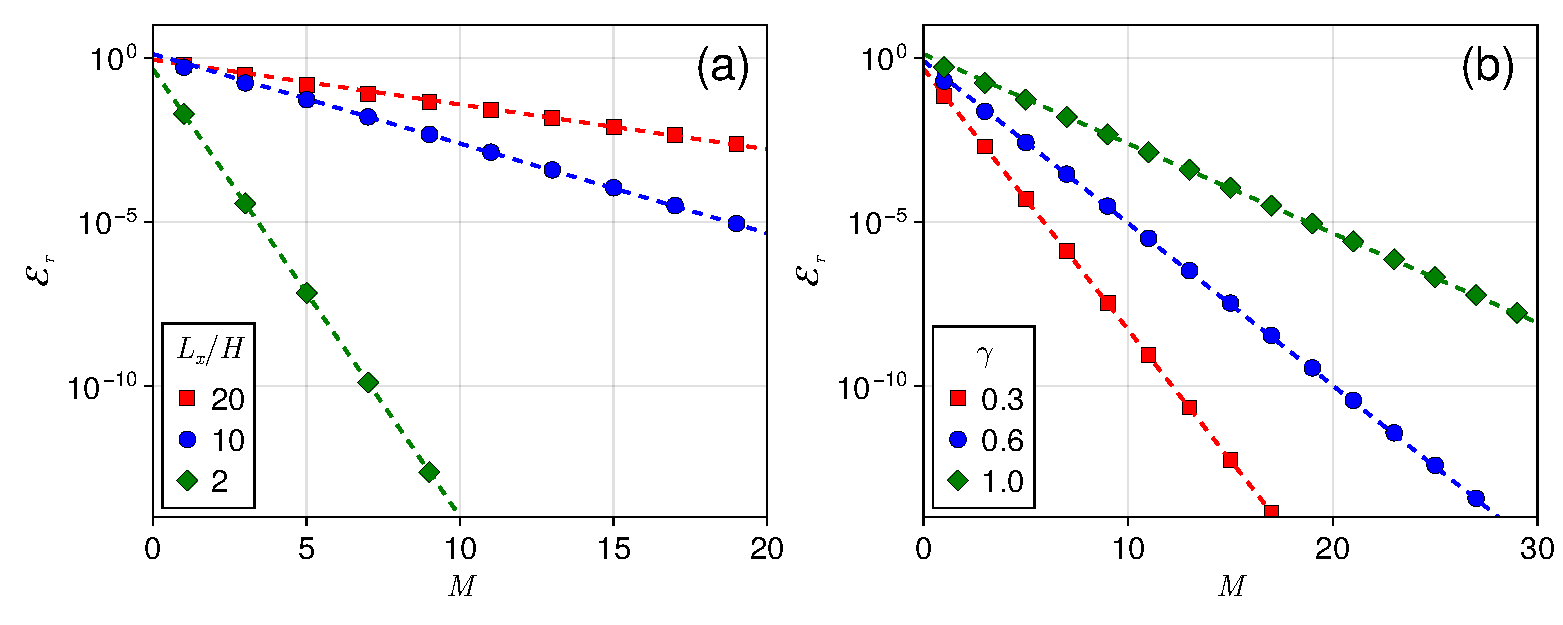
\includegraphics[width=0.98\linewidth]{figs/icm_error_force.pdf}
    \caption{
        Relative errors in force ($\mathcal{E}_r$) as a function of the truncation parameter $M$ for the image charge series. 
        The dashed lines represent the fitted curves with decay rates using our theoretical prediction Eq.~\eqref{eq::Ferr1}. 
        In panel (a), we fix $\gamma_{\T u} = \gamma_{\T d} = 1$ and consider systems with varying heights $H = 0.5$, $1$, and $5$. In panel (b), we fix $H = 1$ while varying $\gamma_{\T u} = \gamma_{\T d} = \gamma$ with values of $0.3, 0.6,$ and $1$. In both panels, we fix $L_x=L_y=10$.
    }
    \label{fig:icm_error_force}
\end{figure}

\subsection{Estimations of ELC term with image charges}\label{sec:error_reform}

Another often-overlooked source of error in existing algorithms stems from the omission of the ELC term in Eq.~\eqref{eq:U^M_ELC} and the discretization error using the trapezoidal rule, which has been discussed in Section~\ref{sec::icm_ewald2d}. 
In this section, we focus on deriving estimations of the ELC term with image charges.
%a rough estimation has been given as the following Lemma~\cite{gan2024fast}.

First, we recall the definition of the ELC term with image charges, denoted as $U_{\text{ELC}}^{M}$, as provided in the energy expressions Eqs.~\eqref{eq:U^M_ELC} and~\eqref{eq::23}:
\begin{equation}\label{eq::UELCm}
U_{\T {ELC}}^{M}:=\frac{2\pi}{L_xL_y}\sum_{i,j=1}^{N}q_iq_j\sum_{\bm{h}\neq \bm{0}} \frac{e^{\i \bm{h}\cdot\bm{r}_{ij}}e^{-hL_z}\left[\cosh(hz_{ij})+\mathscr{F}_{\text{ELC}}^{M}(z_i,z_j)\right]}{h(e^{-hL_z}-1)}\;.
\end{equation}
To derive an estimation for $U_{\T {ELC}}^{M}$, we introduce the following two inequalities. 
1). By basic algebraic manipulations, one obtains:  
\begin{equation}\label{eq::bpud1}
e^{-hL_z}\cosh(hz_{ij})\leq e^{-h(L_z-|z_{ij}|)}\leq e^{-h(L_z-H)}\;,
\end{equation}
and 2).
\begin{equation}\label{eq::bpud2}
\begin{split}
& e^{-hL_z}\mathscr{F}_{\text{ELC}}^{M}(z_i,z_j) \\
= & e^{-hL_z}\sum\limits_{l=1}^{M}\left[\gamma_{+}^{(l)}\cosh(h(z_i-z_{j+}^{(l)}))+\gamma_{-}^{(l)}\cosh(h(z_i-z_{j-}^{(l)}))\right]\\
= & \frac{1}{2}\sum\limits_{l=1}^{M}\left[\gamma_{+}^{(l)}e^{-h(L_z-|z_i-z_{j+}^{(l)}|)}+\gamma_{-}^{(l)}e^{-h(L_z-|z_i-z_{j-}^{(l)}|)}\right]+\frac{e^{-hL_z}}{2}(\mathcal{G}_{0}(z_i,z_j)-\mathcal{G}_{M}(z_i,z_j))\\
\leq & \frac{1}{2}\sum_{l=1}^{M}C^{(l)}_{\gamma}e^{-h(L_z-(l+1)H)}+\frac{(|\gamma_{\T u}|+|\gamma_{\T d}| + 2|\gamma_{\T u}\gamma_{\T d}|)e^{-hL_z}}{1-|\gamma_{\T u}\gamma_{\T d}|e^{-2hH}},
\end{split}
\end{equation}
where the factor $C^{(l)}_{\gamma}$ is defined as 
\begin{equation}
C^{(l)}_{\gamma}:=\left|\gamma_{+}^{(l)}\right|+\left|\gamma_{-}^{(l)}\right|=\left| \gamma_{\T d}^{\lceil l/2 \rceil} \gamma_{\T u}^{\lfloor l/2 \rfloor}\right|+\left| \gamma_{\T d}^{\lfloor l/2 \rfloor} \gamma_{\T u}^{\lceil l/2 \rceil}\right|.
\end{equation}
To obtain the above inequality, we use the definitions of $\gamma_{+}^{(l)}$ and $\gamma_{-}^{(l)}$, the bound $\max_{i,j}\{|z_i-z_{j+}^{(l)}|,|z_i-z_{j-}^{(l)}|\}\leq (l+1)H$, and the definition of $\mathcal{G}_{M}(z_i,z_j)$ in Eq.~\eqref{eq::rGrrij} along with its bound given in Eq.~\eqref{eq:beta_ij}. 
Substituting Eqs.~\eqref{eq::bpud1} and \eqref{eq::bpud2} into Eq.~\eqref{eq::UELCm} yields

\begin{equation}
\resizebox{.98\hsize}{!}{$
\begin{split}
\left|U_{\text{ELC}}^{M}\right|&\leq \frac{2\pi}{L_xL_y}\sum_{\bm{h}\neq \bm{0}} \frac{C_q\left[e^{-h(L_z-H)}+\frac{1}{2}\sum\limits_{l=1}^{M}C^{(l)}_{\gamma}e^{-h(L_z-(l+1)H)}+\frac{(|\gamma_{\T u}|+|\gamma_{\T d}| + 2|\gamma_{\T u}\gamma_{\T d}|)e^{-hL_z}}{1-|\gamma_{\T u}\gamma_{\T d}|e^{-\frac{4\pi H}{\max\{L_x,L_y\}}}}\right]}{h(1-e^{-\frac{2\pi L_z}{\max\{L_x,L_y\}}})}\\
&\leq \frac{4\pi^2 C_q}{L_xL_y(1-e^{-\frac{2\pi L_z}{\max\{L_x,L_y\}}})}\int^{\infty}_{\frac{2\pi}{\max\{L_x,L_y\}}} \left[e^{-h(L_z-H)}+\sum\limits_{l=1}^{M}\frac{C^{(l)}_{\gamma}}{2}e^{-h(L_z-(l+1)H)}+\frac{4e^{-hL_z}}{1-e^{-\frac{4\pi H}{\max\{L_x,L_y\}}}}\right]dh\\
&=\frac{4\pi^2 C_q}{L_xL_y(1-e^{-\frac{2\pi L_z}{\max\{L_x,L_y\}}})}\left[\frac{e^{-\frac{2\pi(L_z-H)}{\max\{L_x,L_y\}}}}{L_z-H}+\sum_{l=1}^{M}\frac{C_{\gamma}^{(l)}e^{-\frac{2\pi(L_z-(l+1)H)}{\max\{L_x,L_y\}}}}{2(L_z-(l+1)H)}+\frac{4e^{-\frac{2\pi L_z}{\max\{L_x,L_y\}}}}{L_z(1-e^{-\frac{4\pi H}{\max\{L_x,L_y\}}})} \right],
\end{split}
$}
\end{equation}
where we recall $C_q$ is the bound of $|\sum_{i,j=1}^{N}q_iq_je^{\i \bm{h}\cdot\bm{r}_{ij}}|$, $\left|\gamma_{\T u}\right|\leq 1$, and $\left|\gamma_{\T d}\right|\leq 1$. 
Finally, suppose $L_z>(M+1)H$, we obtain the following estimation for the ELC contribution in energy, $U_{\text{ELC}}^{M}$, as:
\begin{equation}
\label{eq::U_ELC}
\left|U_{\text{ELC}}^{M}\right|\sim O\left(e^{-\frac{2\pi(L_z-H)}{\max\{L_x,L_y\}}}+\sum_{l=1}^{M}C_{\gamma}^{(l)}e^{-\frac{2\pi(L_z-(l+1)H)}{\max\{L_x,L_y\}}}\right).
\end{equation}

The corresponding ELC term in force calculations can be estimated analogously. 
We have
\begin{equation}
\left|\bm{F}_{\text{ELC}}^{M,i}\right|:=|-\nabla_{\bm{r}_i} U_{\text{ELC}}^{M}|\leq \left|\frac{4\sqrt{3}\pi}{L_xL_y}q_i\sum_{j=1}^{N}q_j\sum_{\bm{h}\neq \bm{0}} \frac{e^{\i \bm{h}\cdot\bm{r}_{ij}}e^{-hL_z}\left[\cosh(hz_{ij})+\mathscr{F}_{\text{ELC}}^{M}(z_i,z_j)\right]}{1-e^{-hL_z}}\right|\;.
\end{equation}
Further applying the inequalities Eqs.~\eqref{eq::bpud1} and \eqref{eq::bpud2}, we obtain:

\begin{equation}
\resizebox{0.98\hsize}{!}{$
\begin{split}
\left|\bm{F}_{\text{ELC}}^{M,i}\right|\leq &\frac{4\sqrt{3}\pi}{L_xL_y}\sum_{\bm{h}\neq \bm{0}} \frac{C_Q\left[e^{-h(L_z-H)}+\frac{1}{2}\sum\limits_{l=1}^{M}C^{(l)}_{\gamma}e^{-h(L_z-(l+1)H)}+\frac{(|\gamma_{\T u}|+|\gamma_{\T d}| + 2|\gamma_{\T u}\gamma_{\T d}|)e^{-hL_z}}{1-|\gamma_{\T u}\gamma_{\T d}|e^{-\frac{4\pi H}{\max\{L_x,L_y\}}}}\right]}{1-e^{-\frac{2\pi L_z}{\max\{L_x,L_y\}}}}\\
\leq& \frac{8\sqrt{3}\pi^2 C_Q}{L_xL_y(1-e^{-\frac{2\pi L_z}{\max\{L_x,L_y\}}})}\int_{\frac{2\pi}{\max\{L_x,L_y\}}}^{\infty}h\left[e^{-h(L_z-H)}+\frac{1}{2}\sum\limits_{l=1}^{M}C^{(l)}_{\gamma}e^{-h(L_z-(l+1)H)}+\frac{4e^{-hL_z}}{1-e^{-\frac{4\pi H}{\max\{L_x,L_y\}}}}\right]dh\\
=&\frac{8\sqrt{3}\pi^2 C_Q}{L_xL_y(1-J_3)}\left[\frac{1+J_1}{(L_z-H)^2}e^{-J_1}+\sum_{l=1}^{M}\frac{C_{\gamma}^{(l)}(1+J_2^{(l)})}{2(L_z-(l+1)H)^2}e^{-J_2^{(l)}}+\frac{4(1+J_3)}{L_z^2(1-e^{-\frac{4\pi H}{\max\{L_x,L_y\}}})}e^{-J_3}\right]
\end{split}
$}
\end{equation}
where $C_Q$ is the bound of $|q_i\sum_{j=1}^{N}q_je^{-\i \bm{h}\cdot\bm{r}_{ij}}|$ and the coefficients $J_1$, $J_2^{(l)}$ and $J_3$ are defined via
\begin{equation}
J_1=\frac{2\pi(L_z-H)}{\max\{L_x,L_y\}},\quad\; J_2^{(l)}= \frac{2\pi(L_z-(l+1)H)}{\max\{L_x,L_y\}}\quad \;\text{and} \quad \; J_3=\frac{2\pi L_z}{\max\{L_x,L_y\}}.
\end{equation}
As before, by omitting all the prefactors, we arrive at the following estimation for the ELC contribution in force calculations:
\begin{equation}\label{eq::ForceError}
\left|\bm{F}_{\text{ELC}}^{M,i}\right|\sim O\left(e^{-\frac{2\pi(L_z-H)}{\max\{L_x,L_y\}}}+\sum_{l=1}^{M}C_{\gamma}^{(l)}e^{-\frac{2\pi(L_z-(l+1)H)}{\max\{L_x,L_y\}}}\right).
\end{equation}
Clearly, comparing Eq.~\eqref{eq::ForceError} and Eq.~\eqref{eq::U_ELC}, we find that the ELC contribution behaves asymptotically the same for both energy and force calculations.

\subsection{Leading-order analysis of the ELC term}\label{sec::leadingerr}
The theoretical estimations of the ELC term, as presented in Eqs.~\eqref{eq::ForceError} and~\eqref{eq::U_ELC}, behave differently under different system aspect ratios and reflection factors.
In this section, we conduct a detailed analysis of the leading-order contribution of the ELC term across different system parameter scenarios. 
Our focus will be on the analysis of force calculations, a similar approach can be applied to the energy.

First, by introducing two new dimensionless parameters $g_{\T u}:=\gamma_{\T u}e^{\frac{2\pi H}{\max\{L_x,L_y\}}}$ and $g_{\T d}:=\gamma_{\T d}e^{\frac{2\pi H}{\max\{L_x,L_y\}}}$, Eq.~\eqref{eq::ForceError} can be reformulated as
\begin{equation}
   \label{eq::Error_refo}
   \begin{aligned} \left|\bm{F}_{\text{ELC}}^{M,i}\right|&\sim e^{-\frac{2\pi(L_z-H)}{\max\{L_x,L_y\}}} \left[ 1 + \sum_{l=1}^{M} \left( g_{\T u}^{\lfloor \frac{l}{2} \rfloor} g_{\T d}^{\lceil \frac{l}{2} \rceil} + g_{\T u}^{\lceil \frac{l}{2} \rceil} g_{\T d}^{\lfloor \frac{l}{2} \rfloor} \right) \right]\\
   &=e^{-\frac{2\pi(L_z-H)}{\max\{L_x,L_y\}}}\left[(g_{\T u} + g_{\T d} + 2) \sum_{l = 0}^{\lfloor \frac{M - 1}{2} \rfloor} (g_{\T u}g_{\T d})^{l} + ((-1)^{M}+1) (g_{\T u}g_{\T d})^{\lfloor \frac{M}{2} \rfloor} - 1\right]\,.
   \end{aligned}
\end{equation}
From Eq.~\eqref{eq::Error_refo}, it is clear that the leading-order contribution of the ELC term depends on the magnitude of $|g_{\T u}g_{\T d}|$. 
Specifically, i). if $|g_{\T u}g_{\T d}| > 1$, the ELC leading-order term grows exponentially as $M$ increases:
\begin{equation}\label{eq::lhs_bigger1}
   \abs{\V{F}_{\text{ELC}}^{M,i}} =  \left\{
	\begin{aligned}
		& O \left(2 \abs{g_{\T u} g_{\T d}}^{M/2} e^{-\frac{2\pi (L_z - H)}{\max\{L_x,L_y\}}} \right) , & \text{if $M$ is even,}\\
		& O \left( \left(g_{\T u} + g_{\T d}+2\right)\abs{g_{\T u} g_{\T d}}^{\frac{M-1}{2}} e^{-\frac{2\pi (L_z -H)}{\max\{L_x,L_y\}}} \right) , & \text{if $M$ is odd.}
	\end{aligned}
	\right.
\end{equation} 
ii). If $|g_{\T u}g_{\T d}|=1$, the ELC leading-order term grows linearly with $M$:
\begin{equation}
\label{eq::lhs_1}
\abs{\V{F}_{\text{ELC}}^{M,i}} = O \left( \frac{M}{2}\left(g_{\T u} + g_{\T d}+2\right)e^{-\frac{2\pi L_z}{\max\{L_x,L_y\}}} \right)\;.
\end{equation}
iii). If $|g_{\T u}g_{\T d}|<1$, the summation in Eq.~\eqref{eq::Error_refo} converges as $M\rightarrow +\infty$, yielding a uniform estimation independent with $M$:
\begin{equation}
\label{eq::lhs_less1}
\abs{\V{F}_{\text{ELC}}^{M,i}} \sim O \left( \left(g_{\T u}+g_{\T d}+2\right)e^{-\frac{2\pi L_z}{\max\{L_x,L_y\}}} \right).
\end{equation}
The preceding analysis indicates that, for a fixed system size \( L_z \) (including vacuum layers), the numerical error associated with neglecting the ELC term exhibits a non-trivial dependence on the number of image charge layers \( M \). 
Specifically, for \( |g_{\T u}g_{\T d}|>1 \), the error grows exponentially with \( M \);
for \( |g_{\T u}g_{\T d}| = 1 \), it grows linearly; and for \( |g_{\T u}g_{\T d}| < 1 \), no error escalation is observed as \( M \) increases.

In what follows, we perform a series of numerical tests to validate our theoretical analysis. 
First, we examine the simplest case, i.e., systems \emph{without} dielectric interfaces by setting $\gamma_{\T u} = \gamma_{\T d} = 0$. 
In our numerical tests, we fix $L_x = L_y = 10$, and vary the system heights by setting $H = 0.5, 1, 5$. 
For clarity, we further introduce the dimensionless \emph{padding ratio} $R$, defined as $P = (L_z - H) / L_x$. 
The results, presented in Fig.~\ref{fig:elc_error_force}, clearly show that the relative errors in force $\mathcal{E}_r$ decay exponentially with $P$. 
Notably, the convergence with respect to $P$ is independent of the specific choice of $H$, aligning with our theoretical predictions in Eq.~\eqref{eq::ForceError}. 
Furthermore, our findings underscore the computational challenges of simulating \emph{strongly-confined} systems, characterized by a high aspect ratio, i.e., $L_x / H$. 
According to Fig.~\ref{fig:elc_error_force}, achieving single- or double-precision relative accuracy requires padding the system in the $z$ direction such that $(L_z - H)/L_x$ reaches around 3 and 5, respectively. For strongly-confined systems, this requires one to set $L_z\gg H$, which can significantly increases the computational cost if grid-based algorithms are used.

\begin{figure}[htbp]
    \centering
    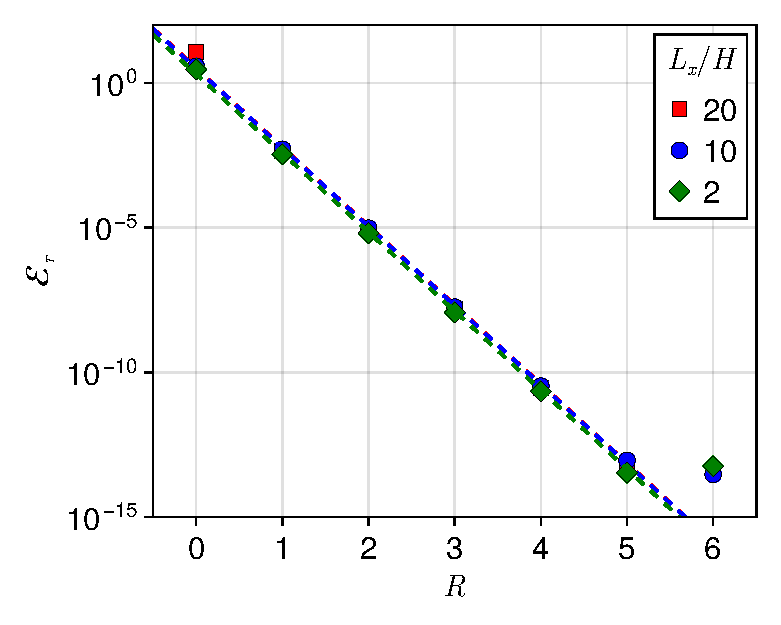
\includegraphics[width=0.55\linewidth]{figs/elc_error_force.pdf}
    \caption{Relative errors in force ($\mathcal{E}_r$) as a function of the padding ratio $R$ for systems without dielectric interfaces. 
    We consider systems with heights $H = 0.5, 1, 5$ while fixing $L_x=L_y=10$. The padding ratio is defined as $R = (L_z - H) / L_x$. The dashed lines represent the fitted curves with decay rates using theoretical prediction Eq.~\eqref{eq::ForceError}. }
    \label{fig:elc_error_force}
\end{figure}

Next, we examine systems with dielectric interfaces.
We set $\gamma_{\T u}=\gamma_{\T d}=\gamma$ and explore two prototypical scenarios by choosing $\gamma = 0.6$ and $1$, respectively. 
In both scenarios, the size of simulation box is fixed as $L_x=L_y=10$ and $H = 0.5$, and we vary the padding ratio $R$ (by changing $L_z$) and the image series truncation parameter $M$ to validate our theoretical results.
We first address the scenario with $\gamma = 0.6$, where we have $|g_{\T u}g_{\T d}| < 1$, so that the numerical errors are mainly contributed by the image series truncation error Eq.~\eqref{eq::Ferr1} and the ELC term Eq.~\eqref{eq::lhs_less1}.
% \begin{equation}\label{eq::0.6}
%     |\bm{F}_{\text{err}}^{M,i}| \sim \max \left\{ \lfloor(M+1)/2\rfloor^{-1}\left|\gamma_{\T u}\gamma_{\T d}\right|^{\lfloor\frac{M+1}{2}\rfloor} e^{-\frac{4\pi H\lfloor (M+1)/2\rfloor}{\max\{L_x,L_y\}}}, ~(g_{\T u}+g_{\T d}+2)e^{-\frac{2\pi L_z}{\max\{L_x,L_y\}}} \right\}\;.
% \end{equation}
The numerical results, as shown in Fig.~\ref{fig:error_icm_pad_gamma_0.6_force}, demonstrate that the errors in force decay exponentially with both the padding ratio $R$ and the number of image charge layers $M$, consistent with our theoretical predictions. Notice that in Fig.~\ref{fig:error_icm_pad_gamma_0.6_force} (a), the errors saturate at certain accuracy levels, this is due to the fixed image series truncation error (as we fix $M$). Similarly, the errors saturate in Fig.~\ref{fig:error_icm_pad_gamma_0.6_force} (b) as they reach the fixed ELC errors for given padding ratios $R$.
\begin{figure}[htbp]
    \centering
    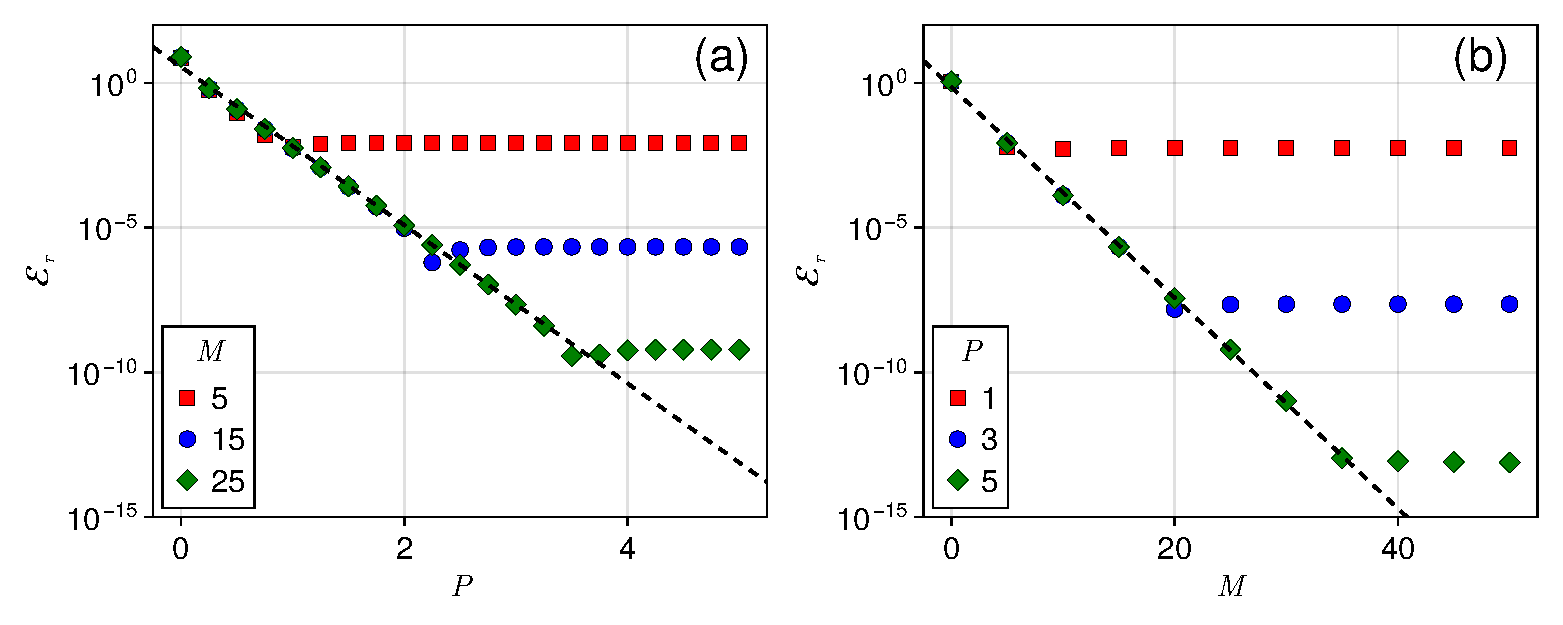
\includegraphics[width=0.98\linewidth]{figs/error_icm_pad_gamma_0.6_force.pdf}
    \caption{Relative errors in force ($\mathcal{E}_r$) for systems with dielectric interfaces. Here we fix $\gamma_{\T u}=\gamma_{\T d}=\gamma = 0.6$, $L_x=L_y=10$ and $H = 0.5$. 
    Panel (a) illustrates errors as a function of padding ratio $R$ with fixed image charge layers ($M=5,~15,~25$); panel (b) illustrates errors as a function of $M$ with fixed padding ratios ($R = 1,~3,~5$). The dashed lines in (a) and (b) represent the fitted curves with decay rates using theoretical predictions Eq.~\eqref{eq::lhs_less1} and Eq.~\eqref{eq::Ferr1}, respectively.}
    \label{fig:error_icm_pad_gamma_0.6_force}
\end{figure}

Now consider the scenario with $\gamma = 1$, where we have $|g_{\T u}g_{\T d}| > 1$, so that the numerical errors associated with the ELC term are described by Eq.~\eqref{eq::lhs_bigger1}.
In this context, the error behavior becomes more complex: as $M$ increases, the ELC error exhibits exponential growth, whereas the image truncation error decreases exponentially.
As illustrated in Fig.~\ref{fig:error_icm_pad_gamma_1_force} (a), by fixing $M$, we still observe exponential convergence in forces as the padding ratio $R$ increases. 
However, for a fixed padding ratio $R$, the errors display non-monotonic behavior with increasing $M$, as depicted in Fig.~\ref{fig:error_icm_pad_gamma_1_force} (b).
This subtle phenomenon was not fully understood since its first observation in the work of Yuan \emph{et al.}~\cite{yuan2021particle}. 
Our analysis reveals it as the combined effect of image truncation and ELC errors: 
initially, errors decrease due to the decay of image truncation errors; and once $M$ surpasses a certain $P$-dependent threshold, the error amplification mechanism predicted by Eq.~\eqref{eq::lhs_bigger1} becomes dominant, causing errors to grow exponentially.
Finally, we note that in strongly-confined systems, the presence of dielectric interfaces would introduce additional computational challenges~\cite{dos2015electrolytes}. 
Specifically, for systems with higher aspect ratios, a larger $M$ is required to achieve the same level of accuracy. The relevant numerical results are summarized in Section 2 of the SI. 
\begin{figure}[htbp]
    \centering
    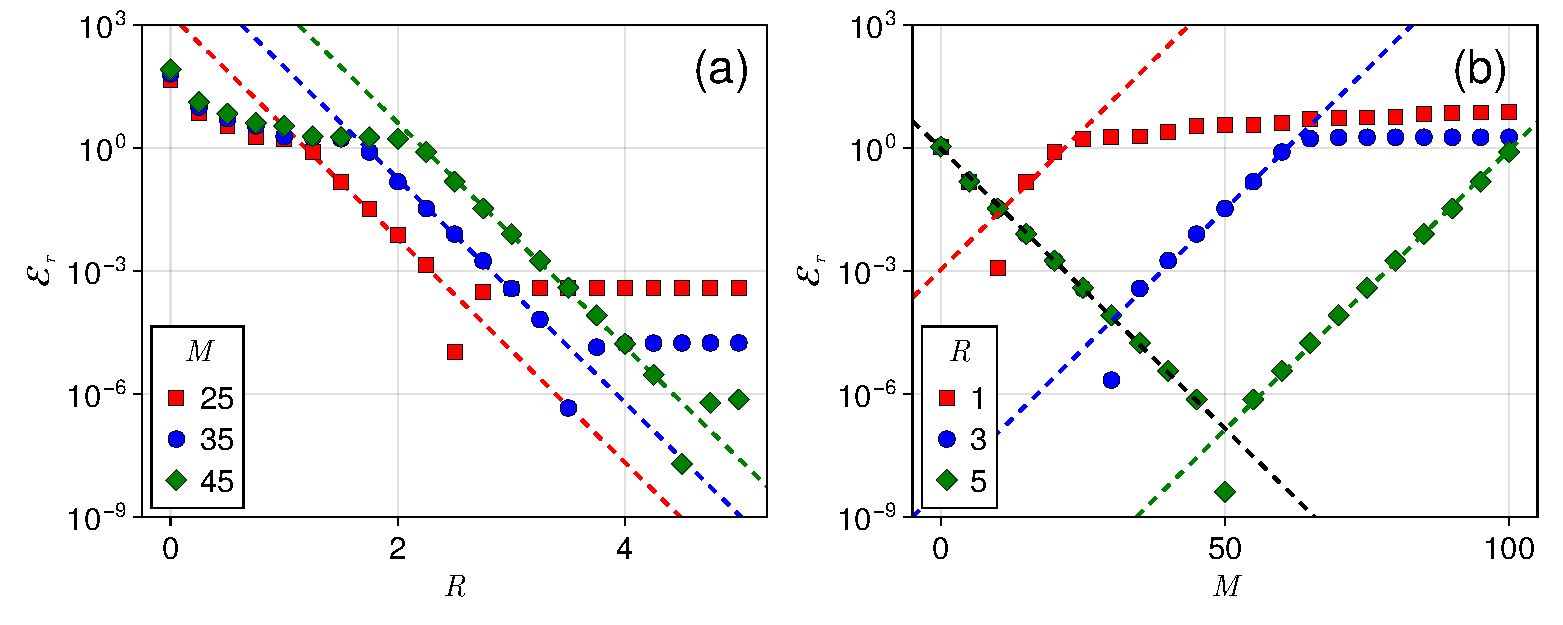
\includegraphics[width=0.98\linewidth]{figs/error_icm_pad_gamma_1_force.pdf}
    \caption{Relative errors in force ($\mathcal{E}_r$) for systems with dielectric interfaces. Here we fix $\gamma_{\T u}=\gamma_{\T d}=\gamma = 1$, $L_x=L_y=10$ and $H = 0.5$. 
    Panel (a) illustrates errors as a function of padding ratio $R$ with fixed image charge layers ($M=25,~35,~45$); panel (b) illustrates errors as a function of $M$ with fixed padding ratios ($R = 1,~3,~5$). The dashed lines in (a) and (b) represent the fitted curves with decay/growth rates using theoretical predictions Eq.~\eqref{eq::lhs_bigger1} and Eq.~\eqref{eq::Ferr1}.}
    \label{fig:error_icm_pad_gamma_1_force}
\end{figure}

% In practical simulations, especially when studying thin membranes, carbon nanotubes, and supercapacitors, accurately capturing the effects of nanoconfinement, i.e., when $H \ll \max\{L_x,L_y\}$, is crucial. Previous works have numerically shown that more image layers are needed to achieve satisfactory accuracy~\cite{dos2015electrolytes}. To further investigate the behavior of strongly confined systems, we present the error in force in \Cref{fig:icm_elc_error_force}, where we set $L_x=L_y=10$, $(L_z-H)/L_x = 5$ and consider system heights $H = 0.5, 1, 5$ while varying the number of image charge layers $M$. In \Cref{fig:icm_elc_error_force} (a), for $\gamma = 0.6$, we observe that the error decays exponentially as $M$ increases for $H = 0.5$ and $H = 1$. However, for $H = 5$, where $\gamma e^{2\pi H / L_x} > 1$, the error initially decreases before increasing as $M$ rises. This behavior is consistent with our theoretical predictions in Eqs.~\eqref{eq::FerrM} and \eqref{eq::FerrModd}. In \Cref{fig:icm_elc_error_force} (b), with $\gamma = 1$, we observe a similar pattern, where the error first decreases and then increases with increasing $M$. Furthermore, we note that the rate of increase depends on the aspect ratio $H/L_x$. A higher aspect ratio leads to a faster increase or decrease in error as $M$ is less or greater than the critical value that minimizes the error, respectively. This is also in alignment with our theoretical results in Eqs.~\eqref{eq::FerrM} and \eqref{eq::FerrModd}.

% \begin{figure}[htbp]
%     \centering
%     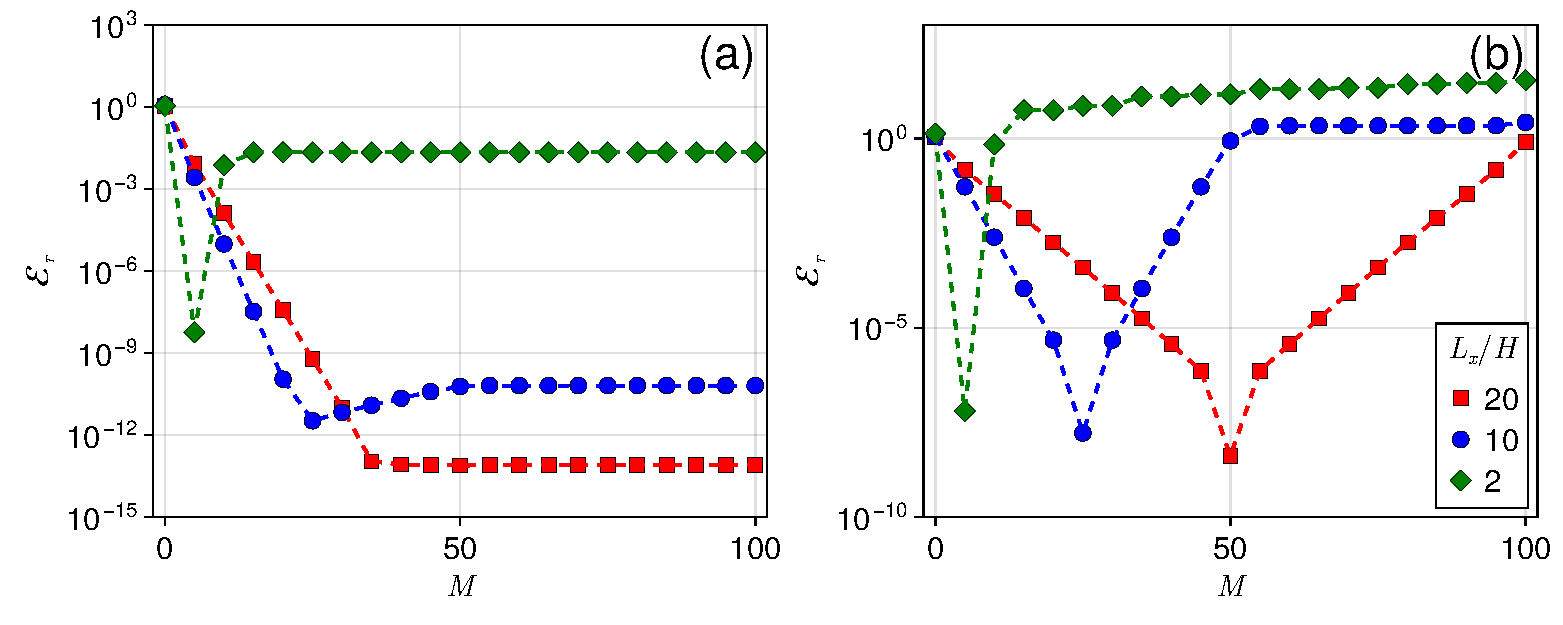
\includegraphics[width=0.98\linewidth]{figs/icm_elc_error_force.pdf}
%     \caption{Relative error of force ($\mathcal{E}_r$) in a dielectric-confined Coulomb system with parameters $P = 5$ and $H = 0.5, 1, 5$. In panels (a) and (b), the dielectric contrasts are set to $\gamma_{\T u} = \gamma_{\T d} = \gamma = 0.6$ and $\gamma_{\T u} = \gamma_{\T d} = \gamma = 1$, respectively.}
%     \label{fig:icm_elc_error_force}
% \end{figure}

As a final example, we validate our theoretical findings by replicating the non-monotonic error behavior reported by Yuan \emph{et al.} in figure 2 of Ref~\cite{yuan2021particle}. 
The reproduced numerical results are shown in Fig.~\ref{fig:error_yuan}, where we examine systems of dielectric-confined 2:1 electrolytes with $L_x = L_y = 15$ and $H = 5$. 
The three panels in Fig.~\ref{fig:error_yuan} correspond to systems with different reflection factors: $\gamma_{\T u} = \gamma_{\T d} = \gamma = 0.6$, $0.95$, and $1$, respectively. 
Within each panel, $L_z$ is varied as $45$, $75$, and $105$.
Note that for all cases considered here, the condition $|g_{\T u}g_{\T d}| > 1$ is satisfied, suggesting a similar phenomenon to that shown in Fig.~\ref{fig:error_icm_pad_gamma_1_force} (b), where errors diverge exponentially as $M$ surpasses a certain threshold.
Finally, we fit the numerical results using an analytical expression that combines the two primary error terms, Eq.~\eqref{eq:Uerr} and Eq.~\eqref{eq::U_ELC}, with coefficients determined through fitting.
The fitted curves, represented by dashed lines in Fig.~\ref{fig:error_yuan}, exhibit excellent agreement with the numerical data, thereby validating our theoretical predictions.

\begin{figure}[htbp]
\centering
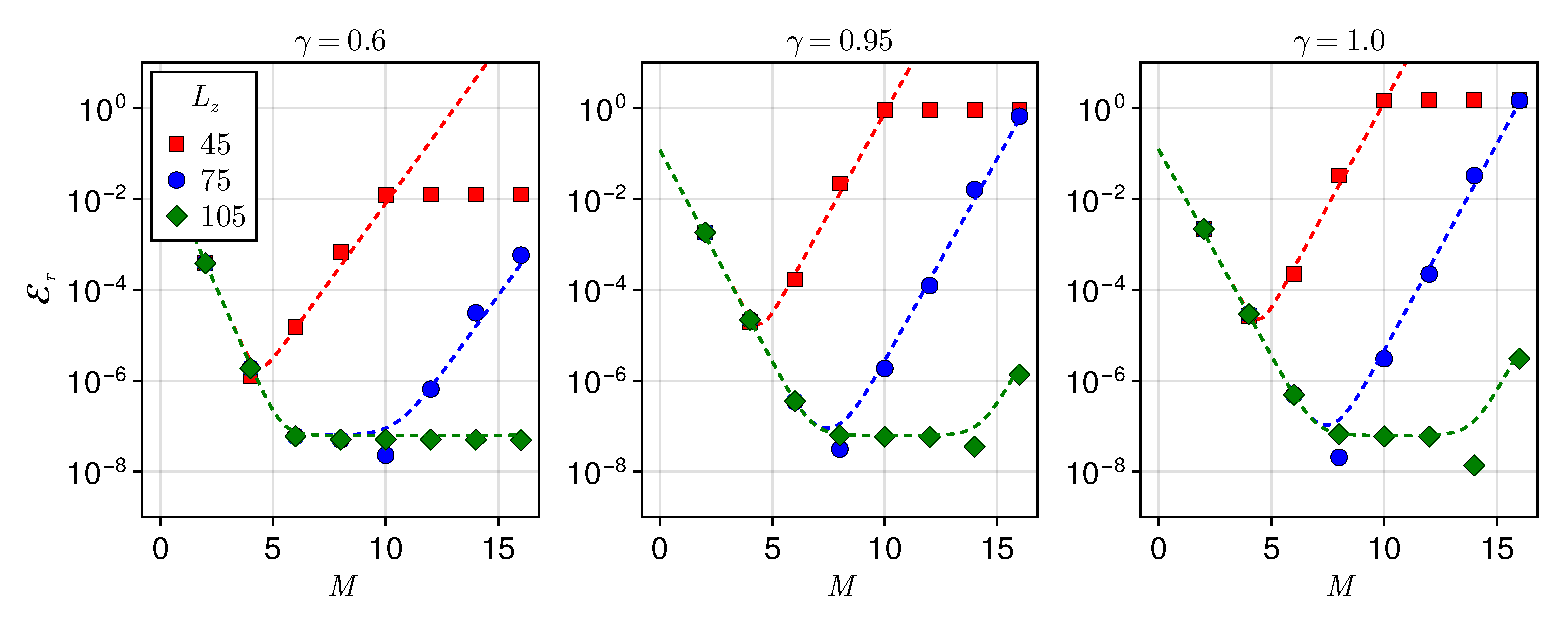
\includegraphics[width=0.98\linewidth]{figs/error_yuan.pdf}
\caption{
Relative errors ($\mathcal{E}_r$) in electrostatic energy for systems of 2:1 electrolytes with dieletric interfaces. 
Here we consider the same system setup studied by Yuan \emph{et al.}~\cite{yuan2021particle} using the ICM-PPPM method with $\gamma_{\T u}=\gamma_{\T d}=\gamma$ = 0.6, 0.95, and 1 (from left to right), respectively. In each panel, we fix $L_x = L_y = 15$, $H = 5$, and consider $L_z=$$45$, $75$, and $105$. 
Finally, the dashed lines represent the fitted curves using the sum of Eqs.~\eqref{eq:Uerr} and~\eqref{eq::U_ELC} (with coefficients determined by fitting).
}
\label{fig:error_yuan}
\end{figure}

\subsection{Optimal parameter selection strategy}\label{sec:parameter}
In practical simulations of dielectric-confined systems, a systematic strategy for determining the optimal algorithm parameters is highly beneficial. Specifically, given a prescribed error tolerance $\varepsilon$, it is crucial to identify parameter choices that achieve this tolerance with minimum computational cost. 
For ICM-Ewald3D~\cite{dos2015electrolytes} and ICM-PPPM~\cite{yuan2021particle} algorithms, 
our error analysis indicates that four interrelated parameters must be determined to control accuracy: 1). the Ewald splitting parameter $\alpha$, 2). the real-space cutoff $r_c$, 3). the image charge series truncation parameter $M$, and 4). the padding length $L_z$. 
By combining the error estimates from this study with the established Ewald splitting error, the overall error estimates for the ICM-Ewald3D and ICM-PPPM methods can be expressed as follows:
\begin{equation}\label{eq:error_icmelc}
\resizebox{0.8\width}{!}{\(
%|U_{\T{err}}|\sim|\bm{F}_{\T{err}}^{i}| 
\varepsilon \sim O\left(\frac{e^{-s^2}}{s^2}+\abs{\gamma_{\T u} \gamma_{\T d}}^{\lfloor\frac{M+1}{2}\rfloor} e^{-\frac{4\pi H \lfloor\frac{(M+1)}{2}\rfloor}{\max\{L_x,L_y\}}} + e^{-\frac{2\pi(L_z-H)}{\max\{L_x,L_y\}}} + \sum\limits_{l=1}^{M}C_{\gamma}^{(l)}e^{-\frac{2\pi(L_z-(l+1)H)}{\max\{L_x,L_y\}}}+e^{-\alpha^2 (L_z-H)^2}\right)\;,
\)}
\end{equation}
where the first term represents the Ewald decomposition error, the second term denotes the image charge series truncation error, the third and fourth terms correspond to the errors associated with the ELC term with image charges, and the last term corresponds to the trapezoidal discretization error.
Recall that, based on our analysis, the fourth term can grow exponentially with increasing $M$ if the condition $|g_{\T u}g_{\T d}| > 1$ is met. 
As a result, one should be careful in properly selecting the parameter $M$. 
Choosing a very large $M$ will not only increase the computational cost, but may also lead to incorrect results under certain circumstances.
In what follows, we propose an optimal parameter selection strategy based on the theoretical guidance of Eq.~\eqref{eq:error_icmelc}.

\emph{Step 1}: select $M$, so that the second term in Eq.~\eqref{eq:error_icmelc} is controlled by $\varepsilon$. 
There are three possible cases depending on the system setups:
\begin{enumerate}
    \item \textbf{Case 1}: If there is no dielectric interface, i.e., $\gamma_{\T u}=\gamma_{\T d}=0$, one simply set $M=0$.
    \item \textbf{Case 2}: If there is only one dielectric interface, i.e., either $\gamma_{\T u}=0$,$~\gamma_{\T d}\neq 0$ or $\gamma_{\T u}\neq 0$,$~\gamma_{\T d}=0$, one can set $M=1$ (since there is no image charge reflection).
    \item \textbf{Case 3}: If there are two polarizable dielectric interfaces, i.e., $\gamma_{\T u}\gamma_{\T d}\neq 0$, we select $M$ according to the following condition (obtained by algebraic manipulations of Eq.~\eqref{eq:Uerr}):
    \begin{equation}\label{eq::38}
    M\sim \frac{2\log \varepsilon - \frac{4\pi H}{\max\{L_x,L_y\}} - \log|\gamma_{\T u} \gamma_{\T d}|}{\log|\gamma_{\T u} \gamma_{\T d}| - \frac{4\pi H}{\max\{L_x,L_y\}}}\;.
\end{equation}
\end{enumerate}

\emph{Step 2}: select $L_z$, such that the sum of the third and fourth terms in Eq.~\eqref{eq:error_icmelc} is controlled by $\varepsilon$. 
Based on the leading-order error analysis presented in Section~\ref{sec::leadingerr}, two cases should be considered: 
\begin{enumerate}
    \item \textbf{Case 1}: If the condition $|g_{\T u}g_{\T d}|=\left|\gamma_{\T u}\gamma_{\T d}e^{\frac{4\pi H}{\max\{L_x,L_y\}}}\right|<1$
is satisfied, we have
\begin{equation}\label{eq::Lz_gamma_u_gamma_d_less1}
    L_z \geq H + \frac{\max\{L_x,L_y\}}{2\pi} \left( \log\frac{1}{\varepsilon} + \log \abs{\gamma_{\T u} + \gamma_{\T d} + e^{- \frac{2\pi H}{\max\{L_x,L_y\}}}} \right)\;.
\end{equation}
Note that for this case, $L_z$ can be chosen independent of $M$.
\item \textbf{Case 2}: If $\left|\gamma_{\T u}\gamma_{\T d}e^{\frac{4\pi H}{\max\{L_x,L_y\}}}\right|\geq 1$, we obtain
\begin{equation}\label{eq::Lz_gamma_u_gamma_d_greater1}
    L_z \geq (M + 1) H + \frac{\max\{L_x,L_y\}}{2\pi} \left( \log\frac{1}{\varepsilon} + \log \abs{\gamma_{\T u} \gamma_{\T d}} \right)\;.
\end{equation}
\end{enumerate}
It is interesting to note that, the selection of $L_z$ as derived in Eq.~\eqref{eq::Lz_gamma_u_gamma_d_greater1} can be interpreted physically as ensuring a sufficiently large vacuum layer in $z$ such that all the image charges can not overlap each other due to the periodic boundary conditions (necessitating $L_z\geq (M+1)H$). Additionally, an extra buffer zone is required, the length of which is determined by the specific tolerance $\varepsilon$.

\emph{Step 3}. After $M$ and $L_z$ are determined, the Ewald splitting parameter $\alpha$ and real-space cutoff $r_c$ can be selected. 
As indicated by Eq.~\eqref{eq:error_icmelc}, the Ewald decomposition error is independent of both the image truncation and the ELC error terms. 
The only extra constraint comes from the trapezoidal discretization error, which is typically minor due to its rapid decay with increasing $L_z$.
Consequently, the standard strategy can be employed to choose these parameters by setting $\varepsilon = e^{-s^2}/s^2$ and solving for $s$, where $s=r_c/\alpha$. 
The specific values of $r_c$ and $\alpha$ can then be adjusted to balance the computational costs between real-space and reciprocal-space calculations~\cite{frenkel2023understanding}.
Finally, to guarantee that the trapezoidal discretization error has been controlled, it is necessary to verify that the following condition is satisfied: 
\begin{equation}
    \alpha \geq (L_z-H)^{-1}\sqrt{\log\varepsilon^{-1}}\;.
\end{equation}
If this condition is not met, then $\alpha$ must be relaxed to fulfill this constraint.

We finally validate the proposed parameter selection strategy through numerical tests on two prototypical dielectric-confined systems, characterized by $\gamma_{\T u} = \gamma_{\T d} = 0.6$ and 1, respectively. 
The system dimensions are fixed at $L_x=L_y=10$ and $H = 1$. 
Note that for the system with $\gamma=0.6$, we have $|g_{\T u}g_{\T d}|<1$, while for the system with $\gamma=1$, $|g_{\T u}g_{\T d}|>1$.
For each system, the error tolerance $\varepsilon$ is set to $\epsilon = 10^{-4}$, $10^{-8}$, and $10^{-12}$. 
By applying the parameter selection strategy discussed earlier, we are able to select the optimized parameters and the results are summarized in Fig.~\ref{tab:parameter_selection_results}. 
Detailed error curves as functions of $M$ and $L_z$ are plotted in Fig.~\ref{fig:error_parameter_selection_force}, where the solid markers denote the specific parameter chosen via the proposed strategy.
\begin{table}[htbp]
    \centering
    \begin{tabular}{|c|c|c|c|c|}
        \hline
        $\gamma$ & $\epsilon$ & $s$ & $M$ & $L_z$ \\
        \hline
        $0.6$ & $10^{-4}$ & 3 & 9 & 15 \\
        $0.6$ & $10^{-8}$ & 4 & 17 & 30 \\
        $0.6$ & $10^{-12}$ & 5 & 25 & 45 \\
        $1$ & $10^{-4}$ & 3 & 16 & 32 \\
        $1$ & $10^{-8}$ & 4 & 31 & 62 \\
        $1$ & $10^{-12}$ & 5 & 45 & 91 \\
        \hline
    \end{tabular}
    \caption{Algorithm parameters $s$,~$M$ and $L_z$ for varied tolerance $\epsilon = 10^{-4}$, $10^{-8}$, and $10^{-12}$. 
    The parameters are selected according to the strategy proposed in this work. Two prototypical dielectric-confined systems are considered, with $\gamma=0.6$ and 1, respectively. Both systems have dimensions $L_x=L_y=10$ and $H = 1$.} \label{tab:parameter_selection_results}
\end{table}
\begin{figure}[htbp]
    \centering
    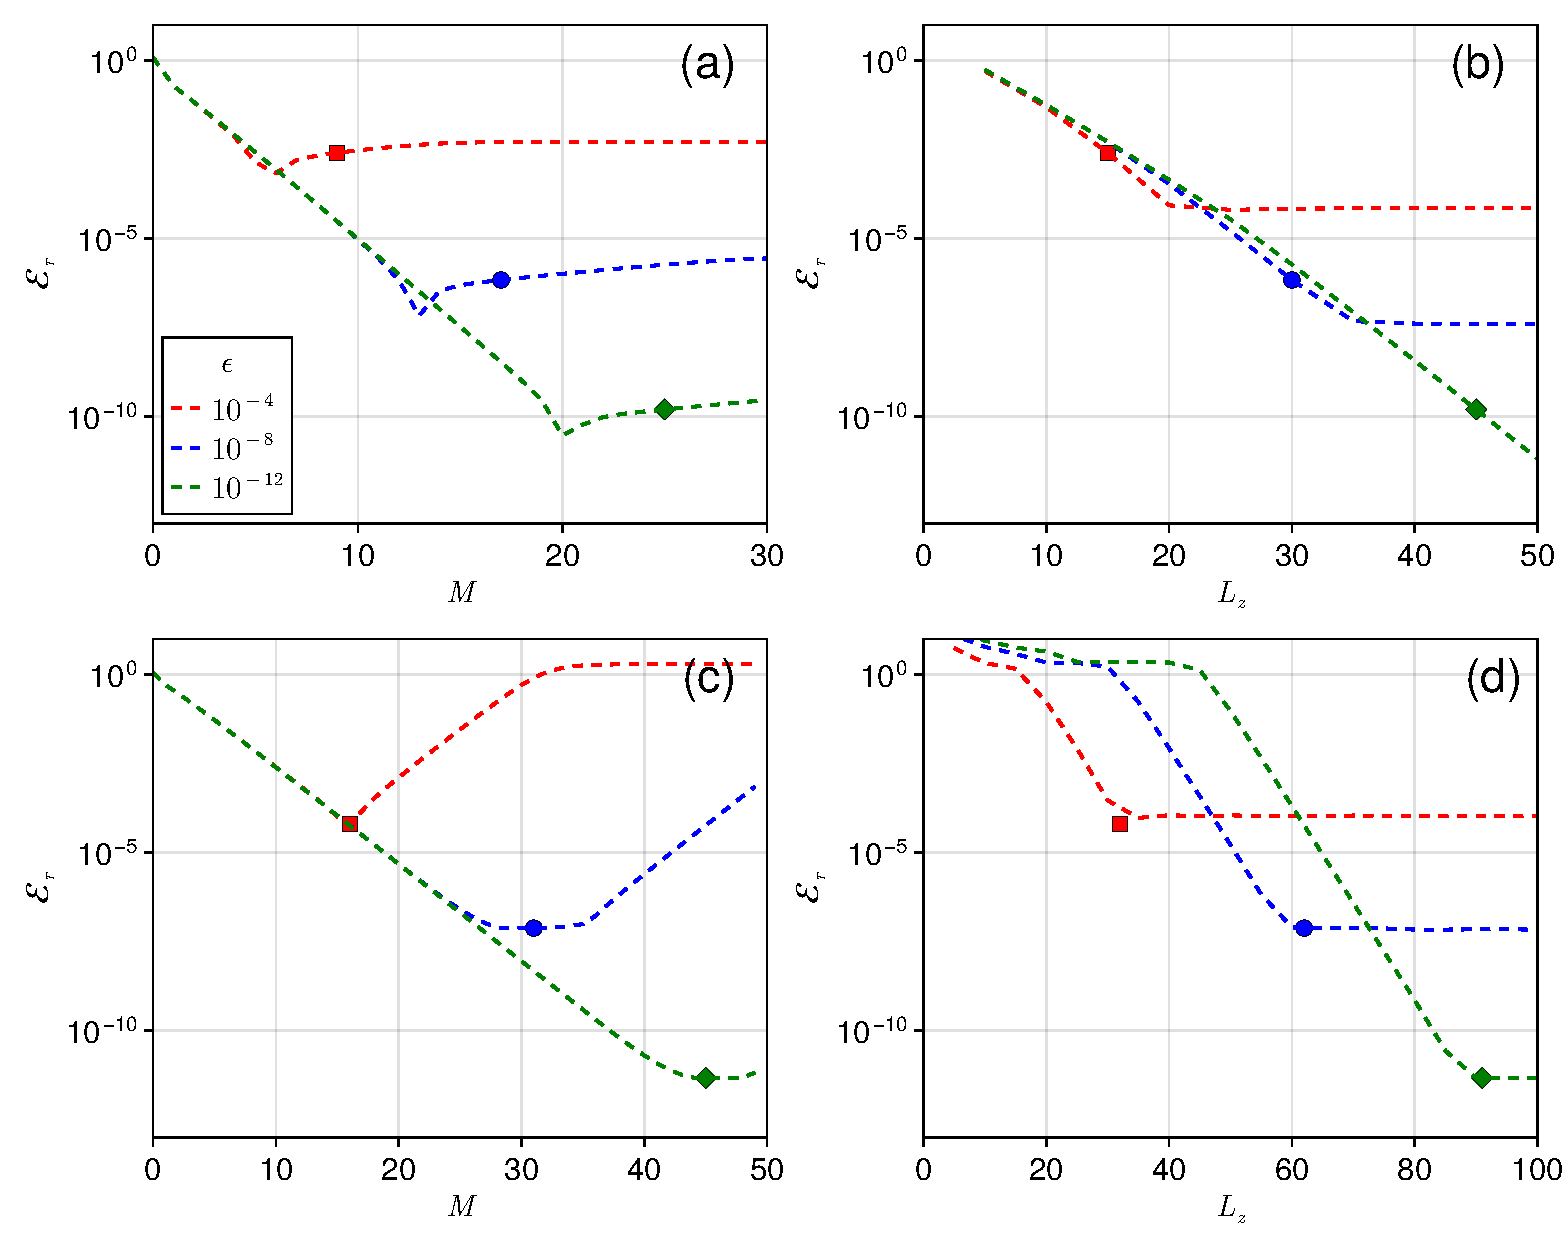
\includegraphics[width=0.92\linewidth]{figs/error_parameter_selection_force.pdf}
    \caption{
        Relative errors in force ($\mathcal{E}_r$) for two prototypical dielectric-confined systems with $\gamma=0.6$ (panels (a-b)) and $\gamma = 1$ (panels (c-d)), respectively.
        For both systems, we fix $L_x=L_y=10$ and $H = 1$. 
        Within each panel, the dashed lines correspond to the numerical errors obtained according to tolerance values $\epsilon = 10^{-4}$, $10^{-8}$, and $10^{-12}$, and the solid markers indicate the specific choice of $M$ or $L_z$ selected via the proposed strategy.
        Note that in panels (a) and (c), $s$ and $L_z$ are fixed according to Fig.~\ref{tab:parameter_selection_results}, whereas in panels (b) and (d), we fix $s$ and $M$.
    }
    \label{fig:error_parameter_selection_force}
\end{figure}
It is evident from Fig.~\ref{fig:error_parameter_selection_force} that, across all test cases with varying $\gamma$ and $\varepsilon$, the selected parameters consistently achieve optimal or near-optimal performance, especially for the case $\gamma = 1$. 
Consequently, we conclude that the parameter selection strategy proposed herein offers practical guidance for optimizing the performance of MD simulations of dielectric-confined systems.
\newpage

\chapter{SOEwald2D for Confined Coulomb Systems in Homogeneous Media}
\label{chp_soewald2d}
In this chapter, we focus on the quasi-2D Coulomb systems in uniform dielectric media, and introduce a fast algorithm named the random batch sum-of-exponentials Ewald2D (RBSE2D) method, which reaches an optimal time complexity of $O(N)$ for the force calculation and can easily handle the systems with large aspect ratios.

\section{Sum-of-exponentials Ewald2D method} \label{sec:method}

In this section, we introduce a novel summation method by using the SOE approximation in evaluating $\xi^{\pm}(h,z)$ and $\partial_{z}\xi^{\pm}(h,z)$. 
This method significantly reduces the overall complexity of Ewald2D to $O(N^{7/5})$ without compromising accuracy. 
Error and complexity analyses are also provided.

%\subsection{The sum-of-exponentials method}
We first give a brief overview of the SOE kernel approximation method.  
For a given precision $\varepsilon$, the objective of an SOE approximation is to find suitable weights $w_l$ and exponents $s_l$ such that~$\forall x \in \mathbb{R}$, the following inequality holds:
\begin{equation}\label{eq::SOE1}
	\left|f(x)-\sum_{l=1}^M w_l e^{-s_l|x|}\right|\leq \varepsilon,
\end{equation}
where $M$ is the number of exponentials. 
Various efforts have been made in literature to approximate different kernel functions using SOE, as documented in works such as~\cite{wiscombe1977exponential, evans1980least, jiang2008efficient, beylkin2005approximation, beylkin2010approximation}.
For instance, the Gaussian kernel $f(x)=e^{-x^2}$ is widely celebrated and plays a crucial role in numerical PDEs~\cite{weideman2010improved,wang2018adaptive}, and is particularly relevant for the purpose of this work. 
The SOE approximation for Gaussians can be understood as discretizing its inverse Laplace transform representation, denoted as
\begin{equation}\label{eq:inverse_laplace}
	e^{-x^2} = \frac{1}{2 \pi \m{i}} \int_{\Gamma} e^{z} \sqrt{\frac{\pi}{z}} e^{-\sqrt{z}\abs{x}} dz\;,
\end{equation}
where $\Gamma$ is a suitably chosen contour. 

% Discretization of the integral in Eq.~\eqref{eq:inverse_laplace} leads to an SOE approximation as given in Eq.~\eqref{eq::SOE1}.
To achieve higher accuracy, several classes of contours have been studied, such as Talbot contours~\cite{lin2004numerical}, parabolic contours~\cite{makarov2000exponentially}, and hyperbolic contours~\cite{lopez2004numerical}. 
An alternative approach is developed by Trefethen, \emph{et al.}~\cite{trefethen2006talbot}, where a sum-of-poles expansion is constructed by the best supremum-norm rational approximants.
A comprehensive review of these techniques has been discussed by Jiang and Greengard~\cite{jiang2021approximating}.
Since the Laplace transform of an SOE is a sum-of-poles expansion~\cite{greengard2018anisotropic}, the model reduction (MR) technique can be employed to further reduce the number of exponentials $M$ while achieving a specified accuracy~$\eps$.
When combining with the MR, convergence rates at $O(6^{-M}) \sim O(7^{-M})$ can be achieved~\cite{jiang2021approximating}.

Additionally, kernel-independent SOE methods have been developed, such as the black-box method~\cite{greengard2018anisotropic} and Vall\'ee-Poussin model reduction (VPMR) method~\cite{gao2021kernelindependent}. 
Specially, the VPMR method integrates the flexibility of Vall\'ee-Poussin sums into the MR technique, demonstrating the highest convergence rate of $O(9^{-M})$ in constructing SOE approximation for Gaussians. 
This method is also bandwidth-controllable and uniformly convergent~\cite{AAMM-13-1126}. 
Due to these advantages, we will utilize the VPMR as the SOE construction tool in all the numerical experiments throughout this paper.


% Moreover, various efforts have been made in the literature to approximate different kernel functions using SOE, as documented in works such as~\cite{wiscombe1977exponential, evans1980least, jiang2008efficient, beylkin2005approximation, beylkin2010approximation}. We do not intend to present a comprehensive review of these algorithms here and refer the reader to these references for further details.

%\begin{rmk}
%It is worth noting that the existing methods for %constructing a sum-of-Gaussians approximation can be %easily extended to constructing an SOE by %incorporating a change of variable $x=\sqrt{t}$.
%\end{rmk}

\subsection{SOE approximations of $\xi^{\pm}(h,z)$} \label{subsec::SOEapp}

To start with, we introduce a useful identity which is a special case of the Laplace transform~(\cite{oberhettinger2012tables}, pp.~374-375; \cite{myint2007linear}, pp.~688). 
\begin{lem}
	Suppose that $a$, $b$, and $c$ are three complex parameters where the real part of $a$ satisfies $\mathscr{R}(a)>0$. For an arbitrary real variable $x$, the following identity holds:
	\begin{equation}\label{eq::identity}
		\int_{x}^{\infty} e^{-(at^2+2bt+c)}dt=\frac{1}{2}\sqrt{\frac{\pi}{a}}e^{(b^2-ac)/a}\erfc\left(\sqrt{a}x+\frac{b}{\sqrt{a}}\right).
	\end{equation}
\end{lem}

Substituting $a=\alpha^2$, $b=h/2$, $c=0$, $x=\pm z$ into Eq.~\eqref{eq::identity} yields the integral representations of $\xi^{\pm}(h,z)$:
\begin{equation}\label{eq::xi20}
	\xi^{\pm}(h,z) = \frac{2\alpha}{\sqrt{\pi}}e^{-h^2/(4\alpha^2)}e^{\pm hz}\int_{\pm z}^{\infty}e^{-\alpha^2t^2-ht} dt \;.
\end{equation}
We then approximate the Gaussian factor $e^{-\alpha^2t^2}$ in the integrand of Eq.~\eqref{eq::xi20} by an $M$-term SOE on the whole real axis, as
\begin{equation}\label{eq::xi21}
	e^{-\alpha^2 t^2} \approx \sum_{l = 1}^M w_{l} e^{ - s_{l} \alpha \abs{t}}\;.
\end{equation}
% That is, for a prescribed precision $\varepsilon$ and a real variable $x$, we assume that
% \begin{equation}\label{eq::SOE1}
	% \left|e^{-x^2}-\sum_{\ell=1}^M w_l e^{-s_l|x|}\right|\leq \varepsilon
	% \end{equation}
% exists where $M$ is the number of exponentials, $w_l$ denotes the weights, and $s_l$ denotes the exponents. 
Inserting Eq.~\eqref{eq::xi21} into Eq.~\eqref{eq::xi20} results in an approximation to $\xi^{\pm}(h,z)$:
\begin{equation}\label{eq::xi_M_int}
	\xi_{M}^{\pm}(h, z) := \frac{2\alpha}{\sqrt{\pi}} e^{-h^2/(4\alpha^2)} e^{\pm hz} \int_{\pm z}^{\infty} \sum_{l = 1}^M w_{l} e^{ - s_{l} \alpha \abs{t}} e^{-ht} dt \;.
\end{equation}
The integral can be calculated analytically (with $\alpha, z > 0$), yielding 
\begin{equation}\label{eq::plus}
	\xi_M^{+}(h,z) = \frac{2 \alpha}{\sqrt{\pi}} e^{-h^2/(4 \alpha^2)} \sum_{l = 1}^M w_l\frac{e^{- \alpha s_l z}}{\alpha s_l + h } 
\end{equation}
and
\begin{equation}\label{eq::minus}
	\xi_{M}^{-}(h, z) = \frac{2 \alpha}{\sqrt{\pi}} e^{-h^2/(4 \alpha^2)} \sum_{l = 1}^M w_l \left[ - \frac{e^{-\alpha s_l z}}{\alpha s_l - h} + \frac{2\alpha s_l e^{- hz}} {(\alpha s_l)^2 - h^2} \right] \;.
\end{equation}
Similarly, one can also obtain the approximation of~$\partial_z \xi^{\pm}(h,z)$, given by
\begin{equation}\label{eq::dz_plus}
	\partial_z \xi_{M}^{+}(h, z) := - \frac{2 \alpha^2 }{\sqrt{\pi}} e^{-h^2/(4 \alpha^2)} \sum_{l = 1}^M w_l s_l \frac{e^{- \alpha s_l z}}{\alpha s_l + h } 
\end{equation}
and
\begin{equation}\label{eq::dz_minus}
	\partial_z \xi_{M}^{-}(h, z) := - \frac{2 \alpha^2}{\sqrt{\pi}} e^{-h^2/(4 \alpha^2)} \sum_{l = 1}^M w_l s_l \left[ - \frac{e^{-\alpha s_lz}}{\alpha s_l - h} + \frac{2 h e^{- hz}} {(\alpha s_l )^2 - h^2} \right] \;.
\end{equation}
The approximation error, which relies on the prescribed precision $\varepsilon$ of the SOE, also has spectral convergence in $h$.
This is summarized in Theorem \ref{thm:error_xi}.

\begin{thm}\label{thm:error_xi}
	Given an $M$-term SOE expansion for the Gaussian kernel $f(x)=e^{-\alpha^2x^2}$ satisfying Eq.~\eqref{eq::SOE1}, the approximation of~$\xi^{\pm}$ derived from Eqs.~\eqref{eq::xi20}-\eqref{eq::minus} has a global error bound
	\begin{equation}\label{eq::bound_xi}
		\abs{\xi^{\pm}(h,z) - \xi_{M}^{\pm}(h, z)} \leq \frac{2 \alpha e^{-h^2/(4 \alpha^2)}}{\sqrt{\pi} h} \varepsilon\;,
	\end{equation}
	and for the approximation of~$\partial_z \xi^{\pm}$ using Eqs.~\eqref{eq::dz_plus}-\eqref{eq::dz_minus}, the error bound is given by
	\begin{equation}\label{eq::bound_dz_xi}
		\abs{\partial_z \xi^{\pm}(h,z) - \partial_z \xi_{M}^{\pm}(h, z)} \leq \frac{4 \alpha e^{-h^2/(4 \alpha^2)}}{\sqrt{\pi}} \varepsilon\;,
	\end{equation}
	which is independent of $z$ and decays rapidly with $h$.
\end{thm}

\begin{proof}
	To prove Eq.~\eqref{eq::bound_xi}, one can directly subtract Eq.~\eqref{eq::xi_M_int} from  Eq.~\eqref{eq::xi20} to obtain:
	\begin{equation}
		\begin{split}
			&\abs{\xi^{\pm}(h, z) - \xi_{M}^{\pm}(h, z)}\\
			\leq & \frac{2 \alpha}{\sqrt{\pi}} e^{-h^2/(4 \alpha^2)} \int_{\pm z}^\infty e^{\pm hz - h t} \abs{e^{-\alpha^2 t^2} - \sum_{l = 1}^M w_l e^{-\alpha s_l\abs{t}} } dt \\
			\leq & \frac{2 \alpha}{\sqrt{\pi}} e^{ - h^2/(4 \alpha^2)} \varepsilon \int_{\pm z}^\infty e^{\pm hz - h t} dt \\
			= & \frac{2 \alpha e^{-h^2/(4 \alpha^2)}}{\sqrt{\pi} h} \varepsilon\;,
		\end{split}
	\end{equation}
	where from the second to the third line, one uses the boundness of SOE approximation error, i.e., Eq.~\eqref{eq::SOE1}.
	For the approximation error of $\partial_z\xi^{\pm}$, the proof is similar. One can subtract the $z$-derivative of Eq.~\eqref{eq::xi_M_int} from the $z$-derivative of Eq.~\eqref{eq::xi20} to obtain
	\begin{equation}
	\begin{split}
	& \abs{\partial_z \xi^{\pm}(h, z) - \partial_z \xi_{M}^{\pm}(h, z)}\\
	\leq & \frac{2 \alpha}{\sqrt{\pi}} e^{-h^2/(4 \alpha^2)} \left( \int_{\pm z}^\infty h e^{\pm hz - h t} \abs{e^{-\alpha^2 t^2} - \sum_{l = 1}^M w_l e^{-\alpha s_l\abs{t}} } dt + \abs{e^{-\alpha^2 z^2} - \sum_{l = 1}^M w_l e^{-\alpha s_l\abs{z}} } \right)\\
	\leq & \frac{2 \alpha}{\sqrt{\pi}} e^{ - h^2/(4 \alpha^2)} \varepsilon \left( h \int_{\pm z}^\infty e^{\pm hz - h t} dt + 1 \right) \\
	= & \frac{4 \alpha e^{-h^2/(4 \alpha^2)}}{\sqrt{\pi}} \varepsilon\;.
	\end{split}
	\end{equation}
	Again, the boundness of the SOE approximation error is used in the proof, i.e., from the second to the third line.
\end{proof}


For the $\V 0$-th frequency term Eq.~\eqref{eq:phil0} consisting of $\erf(\cdot)$ and Gaussian functions, a similar approach can be employed to construct the corresponding SOE expansions. One has
\begin{equation}\label{eq:SOErf}
	\begin{split}
		\erf(\alpha z)\approx \frac{2}{\sqrt{\pi}} \int_0^{\alpha z} \sum_{l = 1}^M w_l e^{-s_l t} dt= \frac{2}{\sqrt{\pi}} \sum_{l = 1}^M \frac{w_l}{s_l} (1 - e^{- \alpha s_l z})\;.
	\end{split}
\end{equation}
One can prove that
\begin{equation}\label{eq::erfSOE}
	\left|\erf(\alpha z)-\frac{2}{\sqrt{\pi}} \sum_{l = 1}^M \frac{w_l}{s_l} (1 - e^{- \alpha s_l z})\right|\leq \frac{2\alpha H}{\sqrt{\pi}}\varepsilon\;,
\end{equation}
where one assumes that $z\in[0, H]$, as for quasi-2D systems all particles are confined within a narrow region in $z$. 

The advantages and novelty of our SOE approach are summarized as follows.
Firstly, Theorem~\ref{thm:error_xi} demonstrates that the approximation error of our SOE method is uniformly controlled in $z$ and decays exponentially in $k$. Secondly, the resulting approximation $\xi_{M}^{\pm}$ is well-conditioned, thus addressing the issue of catastrophic error cancellation when evaluating $\xi^{\pm}$. 
Achieving these properties are crucial for the subsequent algorithm design.

\begin{rmk}
	The choice of SOE approximation is not unique. Instead of approximating the Gaussian factor in the integrand with an SOE, a more directforward approach might be approximating the complementary error function in~$\xi^{\pm}$ using an SOE. 
	Unfortunately, this will introduce an error proportional to~$e^{hz} \varepsilon$, which grows exponentially with~$h$, resulting in a much larger numerical error in the Fourier space summation for the long-range components of Coulomb energy and forces.
\end{rmk}	


\begin{figure}[ht] 
	\centering
	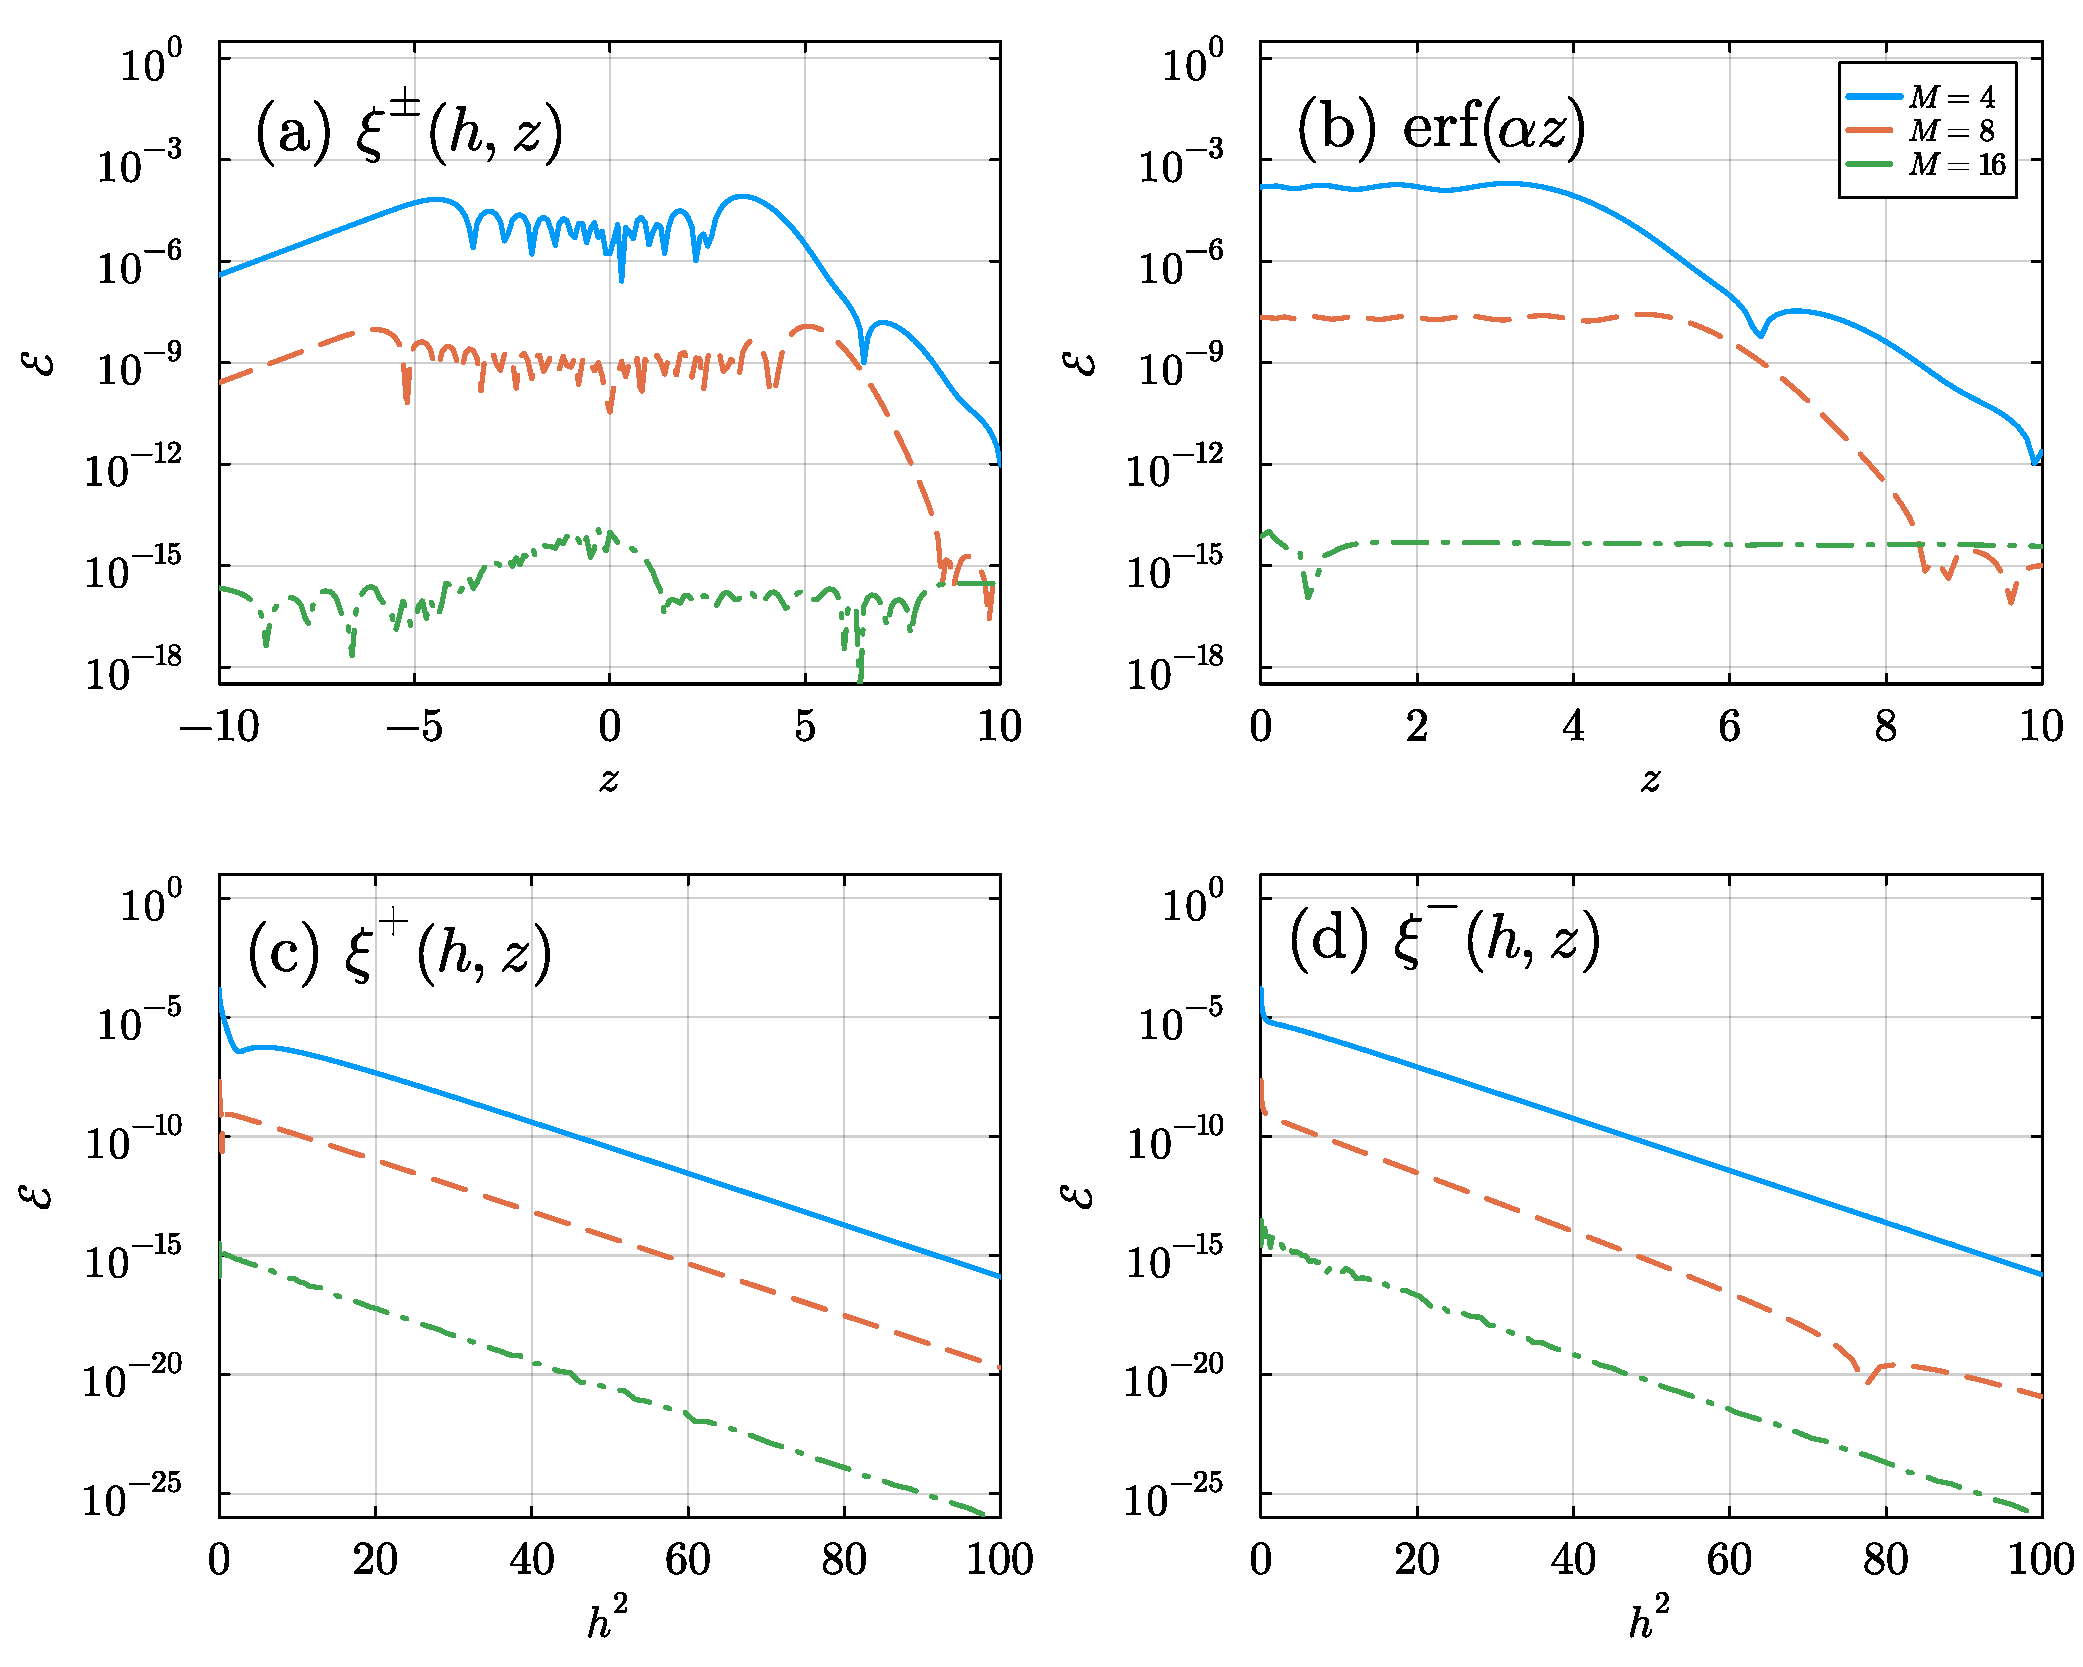
\includegraphics[width=\textwidth]{figs/fig_error_Uxi.pdf}
	\caption{
		The absolute error of the SOE expansion for (a) $\xi^{\pm}(h,z)$ and (b) $\erf(\alpha z)$ is plotted as a function of $z$, while fixing $h=\alpha=1$; absolute error of the SOE expansion of (c) $\xi^{+}(h,z)$ and (d) $\xi^{-}(h,z)$ as a function of $h^2$, while fixing $z=1$.
		Data are presented for SOEs with varying numbers of exponentials, $M=4,$ 8 and 16.
	}
	\label{fig:error_SOE}
\end{figure}

% Analogously, one can approximate the corresponding $z$-derivatives, $\partial_z \xi^{\pm}(k,z)$ and $\partial_z \erf(\alpha z)$ via SOE approximations, which is important in force calculations. The resulting expressions, error estimates, as well as numerical validations are provided in Appendix~\ref{app:dz_ksi}.
% Several advantages in using SOE approximation to reformulate Ewald2D will be further demonstrated, as we proceed to the next section. 
% Both $\xi_{M}^{+}(k, z)$ and $\xi_{M}^{-}(k, z)$ take the form of the SOE with respect to $z$. 
% Comparing with their original forms Eq.~\eqref{eq::9}, the advantages of the SOE-based reformulation are threefold:
% \begin{itemize}
	%     \item[1.] The translational invariance of the exponential function enables variable separation in non-periodic dimension. 
	%     \item[2.] By eliminating all terms of the form $e^{kz}$, the issue of catastrophic error cancellation is effectively addressed.
	%     \item[3.] Similar to the fully-periodic case~\cite{Ewald1921AnnPhys,jin2021random}, the explicit decay factor $e^{-k^2/(4\alpha^2)}$ allows for the construction of fast algorithms to accelerate computations in the first two periodic dimensions. 
	% \end{itemize}
% These advantages will be further demonstrated.

\subsection{SOEwald2D summation and its fast evaluation}\label{subsec::reforEwald2}
In this section, we derive the SOE-reformulated Ewald2D (SOEwald2D) summation, and the corresponding fast evaluation scheme. 
Let us first consider the contribution of the $\V{h}$-th mode $(\V h \neq \V{0})$ to the long-range interaction energy, denoted as $U_{\ell}^{\V{h}}$, which can be written in the following pairwise summation form 
\begin{equation}\label{eq::pairssum8}
	\begin{split}
		U_{\ell}^{\V{h}} = \frac{1}{2} \sum_{i = 1}^N q_{i} \phi^{\V{h}}_\ell(\V{r}_{i}) =\frac{\pi}{L_xL_y}\sum_{1\leq j<i\leq N}q_{i}q_{j} \varphi^{\bm{h}} (\bm{r}_{i},\bm{r}_{j}) + \frac{Q \pi}{h L_x L_y} \erfc\left(\frac{h}{2 \alpha}\right)\;,
	\end{split}
\end{equation}
where we define
\begin{equation}\label{eq:varphi_k}
	\varphi^{\bm{h}}(\bm{r}_{i},\bm{r}_{j}):=\frac{e^{\m{i} \V{h} \cdot \V{\rho}_{ij}}}{h} \left[\xi^{+}(h, z_{ij})+\xi^{-}(h, z_{ij})\right].
\end{equation}
Substituting the SOE approximation of $\xi^{\pm}(h,z)$ described in Eqs.~\eqref{eq::plus} and \eqref{eq::minus}, a new SOE-based formulation can be obtained, denoted as $U_{\ell,\text{SOE}}^{\V{h}}$. 
This approximation is achieved by substituting $\varphi^{\bm{h}}(\bm{r}_{i},\bm{r}_{j})$ with
\begin{equation}\label{eq::SOEphi}
	\begin{split}
		\varphi^{\bm{h}}_{\text{SOE}}(\bm{r}_{i},\bm{r}_{j}) & := \frac{e^{\m{i} \V{h} \cdot \V{\rho}_{ij}}}{h} \left[\xi^{+}_M(h, z_{ij})+\xi^{-}_M(h, z_{ij})\right]\\
		&=\frac{2\alpha e^{-h^2/(4\alpha^2)}}{\sqrt{\pi}h}e^{\m{i}\V{h} \cdot \V{\rho}_{ij}} \sum_{\ell = 1}^{M}  \frac{w_l}{\alpha^2 s_l^2 - h^2}\left( 2 \alpha s_l e^{-h z_{ij}} - 2ke^{-\alpha s_l z_{ij}}\right) \;.
	\end{split}
\end{equation}

For the $\V 0$-th mode contribution $U_{\ell}^{\V{0}}$, an SOE-based reformulation can be similarly obtained according to Eq.~\eqref{eq:SOErf}:
\begin{equation}\label{eq::Ul0SOE}
	U_{\ell,\text{SOE}}^{\bm{0}} = \frac{1}{2} \sum_{i = 1}^N q_{i} \phi^{\bm{0}}_\ell(\V{r}_{i}) = - \frac{2\pi}{L_xL_y}\sum_{1\leq j < i \leq N}q_{i}q_{j}\varphi^{\bm{0}}_{\text{SOE}}(\bm{r}_{i},\bm{r}_{j})-\frac{\pi Q}{\alpha L_xL_y},
\end{equation}
where
\begin{equation}\label{eq::32}
	\varphi^{\bm{0}}_{\text{SOE}}(\bm{r}_{i},\bm{r}_{j}):=\sum_{l=1}^{M}\frac{w_l}{\sqrt{\pi}}\left[\frac{2z_{ij}}{s_l}+\left(\frac{1}{\alpha}-\frac{2z_{ij}}{s_l}\right)e^{-\alpha s_l z_{ij}}\right].
\end{equation}

We now present an iterative approach to compute $U_{\ell,\text{SOE}}^{\V{h}}$ for each $\bm{h}$ with $O(N)$ complexity. 
For simplicity, consider pairwise sum in the following form:
\begin{equation}\label{eq::33}
	S = \sum_{1\leq j < i \leq N} q_{i} q_{j} e^{\m{i} \V{h} \cdot \V{\rho}_{ij}} e^{ - \beta z_{ij} }\;,
\end{equation}
where $\beta$ is a parameter satisfying $\mathscr{Re}(\beta)>0$. It is clear that the pairwise sums in both $U_{\ell,\text{SOE}}^{\V{h}}$ and $U_{\ell,\text{SOE}}^{\V{0}}$ are in the form of Eq.~\eqref{eq::33}, and direct evaluation takes $O(N^2)$ cost. 

To efficiently evaluate $S$, we initially sort the particle indices based on their $z$ coordinates, such that~$i > j \iff z_i > z_j$.
% $z_1 \leq z_2 \leq \cdots \leq z_N$. 
Subsequently, the summation can be rearranged into a separable and numerically stable form:
\begin{align}
	S &=\sum_{i = 1}^N q_{i} e^{\m{i} \bm{h}\cdot\bm{\rho}_{i}}e^{-\beta z_{i}} \sum_{j = 1}^{i - 1} q_{j} e^{-\m{i} \bm{h}\cdot\bm{\rho}_{j}}e^{\beta z_{j}} \label{eq::S0} \\ 
	&= \sum_{i = 1}^N q_{i} e^{\m{i} \bm{h}\cdot\bm{\rho}_{i}}e^{-\beta(z_{i} - z_{i - 1})}A_{i}(\beta)\;, \label{eq::S}
\end{align}
with coefficients
\begin{equation}
	A_{i}(\beta) =  \sum_{j = 1}^{i - 1} q_{j} e^{-\m{i} \bm{h}\cdot\bm{\rho}_{j}}e^{-\beta(z_{i - 1} - z_{j})}\;.
\end{equation}
Clearly, $A_1(\beta)=0,$ $A_2(\beta)=q_1e^{-\m{i} \bm{h}\cdot\bm{\rho}_1}$, and for $i\geq 3$, a recursive algorithm can be constructed to achieve $O(N)$ complexity in computing all the coeffcients:
\begin{equation}\label{eq::35}
	A_{i}(\beta) = A_{i - 1}(\beta) e^{-\beta(z_{i - 1} - z_{i - 2})} + q_{i - 1}e^{-\m{i} \bm{h}\cdot\bm{\rho}_{i-1}}\;,\quad i = 3, \cdots, N.
\end{equation}
One can thus efficiently evaluate $S$ with another $O(N)$ operations by Eq.~\eqref{eq::S} and using the computed coefficients~$\V{A}(\beta) = (A_1(\beta), ..., A_N(\beta))$. 
Consequently, the overall cost for evaluating the pairwise summation in forms of Eq.~\eqref{eq::33} is reduced to $O(N)$.
Besides the iterative method discussed above, it is remarked that different fast algorithms based on SOE for 1D kernel summations have been developed~\cite{jiang2021approximating,GIMBUTAS2020815}, which can also be used under the framework described in this article for the summation in the non-periodic direction.
% The key point lies in finding an SOE that provides accurate approximations for all Fourier modes, as demonstrated in Section~\ref{subsec::SOEapp} of this paper.

\begin{rmk}
	A similar iterative evaluation strategy can be developed based on Eq.~\eqref{eq::S0} instead of Eq.~\eqref{eq::S}, which may seem more straightforward.
	However, it will lead to uncontrolled exponential terms such as $e^{\beta z_{j}}$, affecting the numerical stability.
	The same issue occurs in the original Ewald2D summation.
	In our recursive scheme, by prior sorting of all particles in $z$, it follows that  $z_{i}-z_{i-1} > 0$ and $z_{i-1} - z_{j} \geq 0$ for all $j \leq i - 1$, thus making all exponential terms in Eq.~\eqref{eq::S} with negative exponents, resolving the exponential blowup issue.
	\label{rmk::stable}
\end{rmk}



Finally, the long-range component of Coulomb interaction energy in Ewald2D summation is approximated via:
\begin{equation}\label{eq:U_l_SOE}
	U_{\ell}\approx U_{\ell,\text{SOE}} := \sum_{\bm{h}\neq \bm{0}} U_{\ell,\text{SOE}}^{\bm{h}}+U_{\ell,\text{SOE}}^{\bm{0}},
\end{equation}
where both $U_{\ell,\text{SOE}}^{\bm{h}}$ and $U_{\ell,\text{SOE}}^{\bm{0}}$ can be evaluated efficiently and accurately with linear complexity.
In MD simulations, the force exerts on the $i$-th particle, $\bm{F}_{i}$, plays a significant role in the numerical integration of Newton's equations.
One can similarly develop fast recursive algorithms to evaluate the SOE-reformulated forces,
the detailed expressions for $\bm{F}_{i}$ is summarized in \ref{app::force}.
We finally summarize the SOEwald2D  in Algorithm~\ref{alg:SOEwald2D}. Its error and complexity analysis will be discussed in the next sections.

\begin{algorithm}[ht] 
	\caption{The sum-of-exponentials Ewald2D method}
	\begin{algorithmic}[1]
		% \setstretch{1.15}
		\State \textbf{Input}: Initialize the size of the simulation box $(L_x, L_y, H)$, as well as the positions, velocities, and charges of all particles. Choose a precision requirement $\varepsilon$.  %, proceed to compute the energy defined in Eq.~\eqref{eq:U} along with its corresponding gradient.
		
		\State \textbf{Precomputation stage}: Determine Ewald splitting parameters $\alpha$ and $s$ according to Eq.~\eqref{eq:trunction_error}. Generate real and Fourier space cutoffs by $r_c=s/\alpha$ and $k_c=2s\alpha$, respectively. Construct the SOE approximations of $\xi^{\pm}(h,z)$ and $\erf(\alpha z)$ following Section~\ref{subsec::SOEapp}.
		
		\Procedure\textnormal{SOEwald2D}{}   
		\State Sort all the particles according to their $z$ coordinates, as $z_1 < z_2 < \cdots < z_N$.
		\State Compute~$U_{\ell,\text{SOE}}^{\bm{h}}$ for $|\bm{h}|\leq k_c$ as well as $U_{\ell,\text{SOE}}^{\bm{0}}$ according to Section~\ref{subsec::reforEwald2}. 
		% \State Compute $U_{\text{self}}$ and $U_{\text{p-s}}$ according to Eqs.~\eqref{eq::self} and \eqref{eq::phiionwall}, respectively.
		\State Compute~$U_{s}$ by direct truncation in real space according to Eq.~\eqref{eq:phi_s} with cutoff $r_c$. %\Comment{short-range part}
		\State Compute $U_{\text{self}}$ according to Eqs.~\eqref{eq::self}.
		\State Compute $U = \sum_{|\bm{h}|\leq k_c} U_{\ell, \text{SOE}}^{\bm{h}} + U_{\ell,\text{SOE}}^{\bm{0}} - U_{\text{self}} + U_{s} + U_{\text{p-s}}$.
		\State Compute forces $\bm{F}_{i}$ using a similar procedure as that of $U$.
		\EndProcedure
		
		\State \textbf{Output}: Total electrostatic energy $U$ and forces $\bm{F}_{i}$.
		
	\end{algorithmic}\label{alg:SOEwald2D}
\end{algorithm}

\subsection{Error analysis}\label{subsec::errSOEwald2D}
Here we derive error estimates for the SOEwald2D summation. 
The total error in the interaction energy $U$ consists of the truncation error and the SOE approximation error:
\begin{equation}
	\mathscr{E}_{U} := \mathscr{E}_{U_{s}}(r_c, \alpha) + \mathscr{E}_{U_{\ell}}(r_c, \alpha) + \sum_{\bm{k}\neq\bm{0}}\mathscr{E}_{U_{\ell},\text{SOE}}^{ \bm{h}} + \mathscr{E}_{U_{\ell},\text{SOE}}^{\bm{0}}\;,
\end{equation}
where the first two terms are the truncation error of Ewald2D summation and have already been provided in Proposition~\ref{prop::2.12}. 
The remainder two terms are the error due to the SOE approximation for the Fourier space components, where
\begin{equation}
	\mathscr{E}_{U_{\ell},\text{SOE}}^{\bm{h}}:=U_{\ell}^{\bm{h}}-U_{\ell,\text{SOE}}^{\bm{h}},\quad \text{and}\quad \mathscr{E}_{U_{\ell},\text{SOE}}^{\bm{0}}:=U_{\ell}^{\bm{0}}- U_{\ell,\text{SOE}}^{\bm{0}}.
\end{equation}
Theorem~\ref{thm:SOE_error} provides  upper bound error estimates, when the Debye-H$\ddot{\text{u}}$ckel (DH) theory is assumed (see~\cite{levin2002electrostatic}, and also~\ref{app::Debye}) to approximate the charge distribution at equilibrium.

\begin{thm}
	\label{thm:SOE_error}
	Given a set of SOE parameters $w_l$ and $s_l$ satisfying Eq.~\eqref{eq::SOE1} and a charge distribution satisfying the DH theory, the SOE approximation error for the Fourier component of interaction energy satisfies:
	\begin{equation}\sum_{\bm{h}\neq\bm{0}}\mathscr{E}_{U_{\ell},\text{SOE}}^{\bm{h}} \leq \frac{2 \lambda_D^2 \alpha^3Q}{\sqrt{\pi}}\varepsilon,
		\quad \text{and} \quad
		\mathscr{E}_{U_{\ell},\text{SOE}}^{\bm{0}} \leq \frac{\sqrt{\pi} \lambda_D^2 (1+2\alpha^2H)Q}{\alpha L_xL_y}\varepsilon,
		\label{eq::51}
	\end{equation}
	respectively, where $\lambda_D$ is the Debye length of the Coulomb system. 
\end{thm}

\begin{proof}
	By definitions of $U_{\ell}^{\bm{h}}$ and $U_{\ell,\text{SOE}}^{\bm{h}}$, one has
	\begin{equation}\label{eq::42}
		U_{\ell}^{\bm{h}}-U_{\ell,\text{SOE}}^{\bm{h}}= \frac{\pi}{2 L_xL_y}\sum_{i=1}^{N}\sum_{j\neq i}q_{i}q_{j}\frac{e^{\m{i} \bm{h}\cdot\bm{\rho}_{ij}}}{h}\mathscr{E}_{\xi^{\pm}},
	\end{equation}
	where 
	\begin{equation}\label{eq::44}
		\mathscr{E}_{\xi^{\pm}} := \abs{\xi^{+}(h,z_{ij})-\xi_{M}^{+}(h,z_{ij})} + \abs{\xi^{-}(h,z_{ij})-\xi_{M}^{-}(h,z_{ij})}\;,
	\end{equation}
	By Theorem~\ref{thm:error_xi}, one has
	\begin{equation}
		|\mathscr{E}_{\xi^{\pm}}|\leq\frac{4\alpha e^{-h^2/(4\alpha^2)}}{\sqrt{\pi}h}\varepsilon\;.
	\end{equation}
	Substituting Eq.~\eqref{eq::44} into Eq.~\eqref{eq::42} and using the DH approximation, one gets
	\begin{equation}\label{eq::47}
		\begin{split}   
			\left| \mathscr{E}_{U_{\ell},\text{SOE}}^{\bm{h}} \right| \leq \frac{2\sqrt{\pi} \lambda_D^2 \alpha Q}{L_x L_y} \frac{e^{-h^2 / (4\alpha^2)}}{h^2} \varepsilon.
		\end{split}
	\end{equation}
	To adequately consider the error in Fourier space, the thermodynamic limit is commonly considered~\cite{kolafa1992cutoff,deserno1998mesh}, wherein the sum over wave vectors is replaced by an integral over $\bm{h}$:
	\begin{equation}\label{eq::integral2}
		\sum_{\bm{h}\neq\bm{0}}\approx \frac{L_xL_y}{(2\pi)^2}\int_{\frac{2\pi}{L}}^{\infty}h dh\int_{0}^{2\pi}d\theta,
	\end{equation}
	where $(h,\theta)$ are the polar coordinates and $L=\max\{L_x,L_y\}$. It then follows that
	\begin{equation}
		\sum_{\bm{h}\neq\bm{0}}\mathscr{E}_{U_{\ell},\text{SOE}}^{ \bm{h}}\leq \frac{2\lambda_D^2\alpha^3Q}{\sqrt{\pi}}\varepsilon.
	\end{equation}
	Finally, recalling the SOE approximation errors of $\erf(\cdot)$ and Gaussian functions given by Eqs.~\eqref{eq::erfSOE} and \eqref{eq::SOE1}, one obtains 
	\begin{equation}
		\begin{split}  
			\left|\mathscr{E}_{U_{\ell},\text{SOE}}^{\bm{0}}\right|\leq \frac{\sqrt{\pi} \lambda_D^2 (1+2\alpha^2H)Q}{\alpha L_xL_y}\varepsilon\;.
		\end{split}
	\end{equation}
	This finishes the proof.
	
	%When Eq.~\eqref{eq::integral2} is applied to a Fourier series (say Eq.~\eqref{eq::47}), one can choose a specific $(k,\theta)$ so that the coordinate along $\cos\theta$ of $\bm{k}$ is in the direction of a specific vector $\bm{\rho}$, and $\bm{k}\cdot\bm{\rho}=k\rho \cos\theta$. 
\end{proof}

Based on Proposition~\ref{prop::2.12} and Theorems~\ref{thm:SOE_error}, we conclude that the overall absolute error in $U$ scales as $\mathscr{E}_{U}\sim O(\varepsilon N)$. 
Notably, for systems sharing the same charge distribution, the Coulomb interaction energy $U \sim O(N)$. 
% Notably, while maintaining a constant particle density within the system, $U$ also exhibits an $O(N)$ scaling behavior. 
Thus we anticipate that our method will maintain a fixed relative error in $U$. 
This will be verified through numerical tests in Section~\ref{subsec::errSOE}.

\subsection{Complexity analysis}

Next we analyze the complexity of the SOEwald2D method summarized in Algorithm~\ref{alg:SOEwald2D}. 
The main computational cost is contributed by the following steps: $N$ particle sorting in $z$, the real and reciprocal space summations.
For sorting (Step 4 in Algorithm~\ref{alg:SOEwald2D}), taking advantage of the quasi-2D confinement, various sorting algorithm are suitable, for example, the bucket sorting algorithm~\cite{cormen2022introduction} results in an $O(N)$ complexity.
To achieve an optimal complexity, the cost of the real and reciprocal space summations (Steps 5 and 6) need to be balanced. 
To analyze it, we first define $\rho_{s}$ and $\rho_{\ell}$ by the average densities in the real and Fourier spaces 
\begin{equation}
	\rho_{s}=\frac{N}{L_x L_y H},\quad \text{and} \quad \rho_{\ell}=\frac{L_xL_y}{(2\pi)^2},
\end{equation}
respectively.
The cost $C_s$ for computing the short-range interaction $U_{s}$ scales as
\begin{equation}\label{eq::cs}
	C_{s}=\frac{4\pi}{3}r_c^3\rho_{s}N=\frac{4\pi s^3N^2}{3\alpha^3 L_x L_y H}.
\end{equation}
% Let $M$ stand for the number of exponentials.
Meanwhile, the total cost $ C_{\ell}$ in computing $U_{\ell,\text{SOE}}^{\bm{h}}$ for all $0<|\bm{h}|\leq h_c$ and $U_{\ell,\text{SOE}}^{\bm{0}}$ is given by
\begin{equation}\label{eq::cll}
	C_{\ell} = \pi k_c^2\rho_{\ell}MN = \frac{1}{\pi}s^2 \alpha^2 L_x L_y M N
\end{equation}
since the recursive computation requires $O(MN)$ operations for each $\bm{h}$. 
To balance~$C_{s}$ and~$C_{\ell}$, one takes
\begin{equation}
	\alpha \sim \frac{N^{1/5}}{L_x^{2/5}L_y^{2/5}H^{1/5}},
\end{equation}
leading to the optimal complexity
\begin{equation}\label{eq::70}
	% C_{s} = C_{\ell} \sim O(L_x^{1/5}L_y^{1/5}H^{-2/5}N^{7/5}).
	C_{s} = C_{\ell} \sim O(N^{7/5}).
\end{equation}
The self interaction~$U_{\text{self}}$ (Step 7) can be directly calculated with a complexity of $O(N)$, and cost of summing up the total energy (Step 8) is clearly $O(1)$.
By taking into consideration that the force calculation (Step $9$) requires asymptotically the same cost as the energy calculation (Steps $4$-$8$), it can be concluded that the overall computational complexity of the SOEwald2D algorithm is $O(N^{7/5})$. 
It is clearly much faster than the original Ewald2D method which scales as $O(N^{2})$; and surprisingly, it is even slightly faster than Ewald3D for fully-periodic systems, which scales as $O(N^{3/2})$.

\begin{rmk}\label{rmk::extreme}
	For the extreme case, $H \ll \min\{L_x,L_y\}$, the neighboring region for the short-range interaction reduces to a cylinder with radius $r_c$ due to the strong confinement, rather than a spherical region. 
	In this case, one has:
	\begin{equation}
		C_{s}\sim 2\pi r_c^2 \frac{N}{L_x L_y} N=\frac{2\pi s^2N^2}{\alpha^2L_x L_y H}.
	\end{equation}
	By simple calculation, the optimal complexity is found to be $O(N^{3/2})$, which is the same as that of the Ewald3D summation for fully-periodic problems. 
	% Similarly, when $H\gg \max\{L_x,L_y\}=O(1)$, the optimal complexity is $O(N)$ according to Eq.~\eqref{eq::70}.
\end{rmk}

% In a $N$ particle simulation of quasi-2D Coulomb systems, to further reduce the complexity to  $O(N)$, we further introduce a stochastic approach to efficiently approximate the Fourier component in the periodic dimensions. 
% This approach differs significantly from existing methods that rely on either FFT-~\cite{lindbo2012fast} or FMM-based methods~\cite{pei2023fast} for handling periodicity.

\section{Random batch SOEwald2D method} \label{sec:rbm}

In this section, we will introduce a stochastic algorithm designed to accelerate the SOEwald2D method in particle simulations, reducing the complexity to $O(N)$. 
Unlike existing methods relying on either FFT or FMM-based techniques to reduce the complexity, our idea involves adopting mini-batch stochastic approximation over Fourier modes, with importance sampling for variance reduction. 
More precisely, let us consider the Fourier sum over $\bm{h} \in \mathcal{K}^2$ for a given kernel $f(\bm{h})$,
one can alternatively understand the Fourier sum as an expectation
\begin{equation}
	\mu:=\sum_{\bm{h}\in\mathcal{K}^2}\frac{f(\bm{h})}{g(\bm{h})}h(\bm{h})=\mathbb{E}_{\bm h\sim g(\bm{h})}\left[\frac{f(\bm{h})}{g(\bm{h})}\right],
\end{equation}
where $\mathbb{E}_{\bm h \sim g(\bm{h})}$ denotes the expectation with $\bm{h}$ sampled from a chosen probability measure $g(\bm{h})$ defined on the lattice $\bm h \in \mathcal{K}^2$. 
Instead of calculating the summation directly or using FFT, a mini-batch of Fourier modes (with batch size $P$) sampled from $g(\bm{h})$ are employed to estimate the expectation, resulting in an efficient stochastic algorithm.

However, when formulating algorithms for quasi-2D systems, the direct application of the random mini-batch idea introduces formidable challenges.
The classical Ewald2D, either in the closed form (Eq.~\eqref{eq:philk}) or the integral form (Eq.~\eqref{eq::phil}), are unsuitable for random batch sampling:ee
(1) the closed form demands $O(N^2)$ complexity even with batch size $P \sim O(1)$; 
(2) the integral form is singular at $h = \kappa = 0$, giving rise to significant variance.
In this section, we will show that the idea of random mini-batch can now be easily incorporated into the SOEwald2D algorithm based on the reformulation of Ewald2D proposed in Section~\ref{subsec::reforEwald2}, resulting in the Random Batch SOEwald2D~(RBSE2D) method, which can accurately satisfy the SPMF condition for quasi-2D geometry.
Detailed analyses will also be provided.

% \subsection{Random batch importance sampling}\label{subsec::rbis}
\subsection{The linear complexity stochastic algorithm} \label{subsec::rbis}

% In this section, we will introduce how the idea of random mini-batch sampling is induced into the SoEwald2D method, 

It has been shown in Eqs.~\eqref{eq::pairssum8}, \eqref{eq:varphi_k} and \eqref{eq::SOEphi} that, after applying the SOE approximation to $U_{\ell}^{\bm{h}}$, the Fourier space summation in the SOEwald2D can be compactly written as
\begin{equation}
	\sum_{\bm{h}\neq\bm{0}} U_{\ell,\text{SOE}}^{\bm{h}} = \sum_{\bm{h}\neq\bm{0}} \widetilde{\varphi} (\bm{h})\;,
\end{equation}
where $\widetilde{\varphi} ({\bm{h}})$ is defined as
\begin{equation}
	\widetilde{\varphi} ({\bm{h}}) := e^{-\frac{h^2}{4 \alpha}} \left[ \frac{2\alpha\sqrt{\pi}}{L_xL_y}\sum_{\ell = 1}^{M}  \frac{w_l \sum_{1\leq j < i \leq N}q_{i} q_{j} e^{\m{i}\V{h} \cdot \V{\rho}_{ij}} \left(2\alpha s_l e^{-h z_{ij}}-2h e^{-\alpha s_l z_{ij}}\right) }{h(\alpha^2 s_l^2 - h^2)} \right] \;.
\end{equation}
Comparing to the original Ewald2D formula given in Section~\ref{sec::ewald2d}, one finds a Gaussian decay factor explicitly, which can be normalized for the purpose of importance sampling.
Thus, we take
\begin{equation}\label{eq::hk}
	g(\bm{h}) := \frac{e^{-h^2/(4\alpha^2)}}{S}\quad\text{with}\quad S := \sum_{\bm{h}\neq\bm{0}}e^{-h^2/(4\alpha^2)},
\end{equation}
where $S$ serves as a normalization factor. 
By the Poisson summation formula (see Lemma~\ref{lem::Poisson}), one has 
\begin{equation}\label{eq::Happ}
	S=\frac{\alpha L_xL_y}{\pi}\sum_{m_x,m_y\in\mathbb{Z}}e^{-\alpha(m_x^2L_x^2+m_y^2L_y^2)}-1,
\end{equation}
where $m_{\xi}=L_{\xi}k_{\xi}/2\pi$ with $\xi\in\{x,y\}$. 
The computation of $S$ is cheap, since Eq.~\eqref{eq::Happ} can be simply truncated to obtain a good approximation. 
Generally speaking, $m_{\xi}=\pm 2$ is enough since $\alpha L_{\xi}\gg 1$.
Then using the Metropolis algorithm~\cite{metropolis1953equation, hastings1970monte} (see~\ref{app::Metropolis}), a random mini-batch of frequencies $\{\bm{h}_{\eta}\}_{\eta=1}^P$ is sampled, and the Fourier component of energy can be approximated as:
\begin{equation}\label{eq::RBapp}
	\sum_{\bm{h}\neq\bm{0}} U_{\ell,\text{SOE}}^{\bm{h}} \approx U_{\ell,*}^{\bm{h}\neq\bm{0}} := \frac{S}{P}\sum_{\eta=1}^{P}\widetilde{\varphi}^{\text{RB}}(\bm{h}_{\eta})
\end{equation}
% where~$P$ is the batch size, ~$\{\bm{k}_{\eta}\}_{\eta=1}^P$ is a batch of sampled frequencies
where~$\widetilde{\varphi}^{\text{RB}}({\bm{h}})$ satisfies
\begin{equation}
	\begin{split}
		\widetilde{\varphi}^{\text{RB}}({\bm{h}}) e^{ - \frac{h^2}{4\alpha}} = \widetilde{\varphi}({\bm{h}}) \;,
	\end{split}
\end{equation}
and the corresponding estimator of the force in Fourier space is given by
\begin{equation}
	\sum_{\bm{h}\neq\bm{0}}\bm{F}_{\ell,\text{SOE}}^{\bm{h},i}\approx \bm{F}_{\ell,*}^{\bm{h}\neq\bm{0},i}=-\frac{S}{P} \sum_{\eta=1}^{P}\nabla_{\bm{r}_{i}}\widetilde{\varphi}^{\text{RB}}(\bm{h}_{\eta})\;.
\end{equation}
Each~$\widetilde{\varphi}^{\text{RB}}({\bm{h}})$ and~$\nabla_{\bm{r}_{i}}\widetilde{\varphi}^{\text{RB}}(\bm{h})$ are pairwise summations, fit into the general form of Eq.~\eqref{eq::33}, and can be efficiently computed using the recursive procedure outlined in Eqs.~\eqref{eq::S}-\eqref{eq::35}. 
Due to the use of importance sampling, it is ensured that the aforementioned random estimators are unbiased and have reduced variances, which will be proven in Section~\ref{subsec::consis}.
It is also worth noting that (1) the $\bm h=\bm 0$ mode is excluded in the stochastic approximation and is always computed in an actual MD simulation. Since the averaged potential for the $\bm 0$th mode over the $xy$-plane equal to that of the exact $1/r$ potential, the SPMF condition~\cite{hu2014symmetry} is satisfied (only up to an $O(\varepsilon)$ SOE approximation error); (2) for the  $\bm h\neq \bm 0$ modes, random batch sampling is adopted, and it will be justified that $P$ can be chosen independent of $N$; typically, one can choose $P\sim O(1)$.


In an actual MD simulation, one will utilize these unbiased estimators along with an appropriate heat bath to complete the particle evolution.  
Except for the summation over Fourier modes $\bm{h}$, the methods of the RBSE2D for other components of both energy and force are the same as those in the SOEwald2D, and the algorithm is outlined in Algorithm~\ref{alg:RBSE2D}.
% These aspects as well as the convergence analysis will be provided in the subsequent Section~\ref{subsec::conv}.

We now analyze the complexity of the RBSE2D method per time step. 
Similar to the strategy in some FFT-based solvers~\cite{deserno1998mesh,lindbo2012fast}, one may choose $\alpha$ such that the time cost in real space is cheap and the computation in the Fourier space is accelerated. 
More precisely, one chooses
\begin{equation}\label{eq::59}
	\alpha\sim\frac{N^{1/3}}{L_x^{1/3}L_y^{1/3} H^{1/3}}
\end{equation}
so that the complexity for the real space part is $C_{s}\sim O(N)$. 
By using the random batch approximation Eq.~\eqref{eq::RBapp}, the number of frequencies to be considered is then reduced to $O(P)$ per step, and  the complexity for the Fourier part is $O(PN)$, even for the challenging cases where the system is untra-thin, i.e., $H \ll \min\{L_x,L_y\}$.
These imply that the RBSE2D method has linear complexity per time step if one chooses $P\sim O(1)$, then by selecting $\alpha$ according to Eq.~\eqref{eq::59}, 
% and in comparison with the analysis in Remark~\ref{rmk::extreme}, 
the overall complexity of the RBSE2D is $O(N)$ for all quasi-2D system setups.

\begin{algorithm}[ht] 
	\caption{The random batch sum-of-exponentials Ewald2D method}
	\begin{algorithmic}[1]
		
		\State \textbf{Input}: Initialize the size of the simulation box $(L_x,L_y, H)$, as well as the positions, velocities, and charges of all particles. Choose a precision requirement $\varepsilon$ as well as batch size $P$.
		
		\State \textbf{Precomputation}: Determine Ewald splitting parameters $\alpha$ and $s$ according to Eqs.~\eqref{eq::59} and \eqref{eq:trunction_error}, respectively. Generate real space cutoff by $r_c=s/\alpha$. Construct the SOE approximation of $\xi^{\pm}(h,z)$ and $\erf(\alpha z)$ following Section~\ref{subsec::SOEapp}.
		
		\Procedure\text{RBSE2D}{}       
		\State Draw $P$ frequencies $\{\bm{h}_{\eta}\}_{\eta=1}^{P}$ using the Metropolis algorithm;
		\State Sort all the particles according to their $z$ coordinates, such that $z_1 < z_2 < \cdots < z_N$;
		\State Compute unbiased Fourier space energy $U_{\ell}^{\bm{h}\neq\bm{0},*}$ by importance sampling Eq.~\eqref{eq::RBapp};
		\State Compute SOE-approximated zero-frequency part $U_{\ell,\text{SOE}}^{\bm{0}}$ according to Section~\ref{subsec::reforEwald2}.
		\State Compute $U_{\text{self}}$ and $U_{\text{p-s}}$ via Eqs.~\eqref{eq::self} and \eqref{eq:spectial}, respectively.
		\State Compute~$U_{s}$ by direct truncation in real space via Eq.~\eqref{eq:phi_s} with cutoff $r_c$. %\Comment{short-range part}
		\State Compute $U^{*}=U_{\ell}^{\bm{h}\neq\bm{0},*}+U_{\ell,\text{SOE}}^{\bm{0}}-U_{\text{self}}+U_{s}+U_{\text{p-s}}$.
		\State Compute forces $\bm{F}_{i}^{*}$ via a similar procedure as that of $U^{*}$.
		\EndProcedure
		
		\State \textbf{Output}: Unbiased electrostatic energy $U^{*}$ and forces $\bm{F}_{i}^{*}$.
		
	\end{algorithmic}\label{alg:RBSE2D}
\end{algorithm}



\subsection{Consistency and variance analysis}
\label{subsec::consis}

In this section, we provide theoretical analysis for the RBSE2D method. We start with considering the fluctuations, i.e., the stochastic error introduced by the importance sampling at each time step.
The fluctuations for the Fourier space components of the energy and the force acting on the $i$th particle are defined as follows:
\begin{equation}\label{eq::xichi}
	\Xi := \sum_{\bm{k}\neq\bm{0}}\left( U_{\ell}^{\bm{h}}-U_{\ell,*}^{\bm{h}}\right),\quad\text{and}\quad\V{\chi}_{i} :=\sum_{\bm{h}\neq\bm{0}}\left(\bm{F}_{\ell}^{\bm{h},i}-\bm{F}_{\ell,*}^{\bm{h},i}\right)\;.
\end{equation}
Proposition~\ref{prop:unbaised} is obtained directly by the definition of the importance sampling:
\begin{prop}\label{prop:unbaised}
	$U_{\ell,*}^{\bm{h}\neq\bm{0}}$ and $\bm{F}_{\ell,*}^{\bm{h}\neq\bm{0},i}$ are unbiased estimators, i.e. $\mathbb{E}\Xi= 0$, $\mathbb{E} \V{\chi}_{i} = \bm 0$, and their variances can be expressed by
	\begin{equation}\label{eq::Exi}
		\mathbb{E}\Xi^2=\frac{S}{P}\sum_{\bm{h}_1\neq 0}e^{-k_1^2/(4\alpha^2)}\left|\widetilde{\varphi}^{\text{RB}}(\bm{h}_1)-\frac{1}{S} \sum_{\bm{h}_2\neq 0}\widetilde{\varphi}^{\text{RB}}(\bm{h}_2)e^{-h_2^2/(4\alpha^2)}\right|^2
	\end{equation}
	and
	\begin{equation}\label{eq::Echi}
		\mathbb{E}|\V{\chi}_{i}|^2=\frac{S}{P}\sum_{\bm{h}_1\neq 0}e^{-h_1^2/(4\alpha^2)}\left|\nabla_{\bm{r}_i}\widetilde{\varphi}^{\text{RB}}(\bm{h}_1)-\frac{1}{S} \sum_{\bm{h}_2\neq 0}\nabla_{\bm{r}_i}\widetilde{\varphi}^{\text{RB}}(\bm{h}_2)e^{-h_2^2/(4\alpha^2)}\right|^2.
	\end{equation}
\end{prop}
% The unbiased property in Proposition~\ref{prop:unbaised} implies consistency of the random batch importance sampling. 
% Eqs.\eqref{eq::Exi} and \eqref{eq::Echi} illustrates that the variance of $U_{\ell,*}^{\bm{k}\neq\bm{0}}$ and $\bm{F}_{\ell,*}^{\bm{k}\neq\bm{0},i}$ are bounded and scales as $O(1/P)$. 

Furthermore, under the Debye-H$\ddot{\text{u}}$ckel approximation, one has the following~Lemma~\ref{lem::upper_bound_phiRB} for the upper bounds of random batch approximations.

\begin{lem} 
	Under the assumption of the DH theory, $|\widetilde{\varphi}^{\emph{RB}}(\bm{h})|$ and $|\nabla_{\bm{r}_i}\widetilde{\varphi}^{\emph{RB}}(\bm{h})|$ have upper bounds
	\begin{equation}
		\begin{split}
		\abs{ \widetilde{\varphi}^{\emph{RB}}(\bm{h})} & \leq \frac{2\sqrt{\pi}\lambda_D^2 Q}{L_xL_y h}\left(\sqrt{\pi}+\frac{\alpha \varepsilon}{h}\right),\\
		\abs{\nabla_{\bm{r}_{i}} \widetilde{\varphi}^{\emph{RB}}(\bm{h})} & \leq  \frac{\pi \lambda_D^2 q_{i}^2}{L_xL_y}\left[3+\frac{\alpha}{\sqrt{\pi}}\left(1+\frac{2\sqrt{2}\varepsilon}{h}\right)\right], 
		\end{split}
	\end{equation}
	where $\lambda_{D}$ represents the Debye length.
	\label{lem::upper_bound_phiRB}
\end{lem}
\begin{proof}
	By the definition of $\widetilde{\varphi}^{\text{RB}}(\bm{k})$, one has
	\begin{equation}
		\abs{ \widetilde{\varphi}^{\text{RB}}(\bm{h})}\leq \frac{1}{e^{-h^2/(4\alpha^2)}}\left(\left|U_{\ell,\text{SOE}}^{\bm{h}}-U_{\ell}^{\bm{h}}\right|+\left|U_{\ell}^{\bm{h}}\right|\right)\;.
	\end{equation}
	% where~$U_{\ell}^{\bm{k}}$ is originally defined in Eq.~\eqref{eq::pairssum8}
	An estimation for the first term is given in Theorem~\ref{thm:SOE_error}. 
	To estimate the second term, one may write Eq.~\eqref{eq::pairssum8} as
	\begin{equation}
		U_{\ell}^{\bm{h}} = \frac{\pi}{2 L_x L_y} \sum_{i, j = 1}^N q_i q_j \frac{e^{\m{i} \V{h} \cdot \V{\rho}_{ij}}}{h} \left[ \xi^{+} (h, z_{ij})+\xi^{-} (h, z_{ij}) \right]\;.
	\end{equation}
	Then using the integral representation of $\xi^{\pm}$ Eq.~\eqref{eq::xi20}, one obtains the following estimate
	\begin{equation}\label{eq::118}
		\begin{split}
			e^{\frac{h^2}{4 \alpha^2}} \left[\xi^{+} (h, z)+\xi^{-} (h, z)\right] & = \frac{2\alpha}{\sqrt{\pi}} \left(e^{h z} \int_{z}^{\infty} e^{-\alpha^2 t^2 - ht} dt+e^{-h z} \int_{-z}^{\infty} e^{-\alpha^2 t^2 - ht} dt\right)\\
			& \leq \frac{4\alpha}{\sqrt{\pi}} \int_{- \infty}^{\infty} e^{-\alpha^2 t^2} dt= 4\;.
		\end{split}
	\end{equation}
	By employing the DH approximation, one has
	\begin{equation}
		\abs{ \widetilde{\varphi}^{\text{RB}}(\bm{h})}  \leq  \frac{2\sqrt{\pi}\lambda_D^2 Q}{L_xL_y h} \left(\sqrt{\pi} + \frac{\alpha \varepsilon}{h}\right)\;.
	\end{equation}
	Similarly, by taking $z$-derivative of the integral form of $\xi^{\pm}$, the following estimate holds:
	\begin{equation}\label{eq::estiZ}
		\begin{split}
			e^{\frac{h^2}{4 \alpha^2}} \partial_z \left[\xi^{+} (h, z)+\xi^{-} (h, z)\right] & = \frac{2\alpha}{\sqrt{\pi}} \partial_z \left( e^{\pm h z} \int_{\pm z}^{\infty} e^{-\alpha^2 t^2 - ht} dt \right) \\
			& \leq \frac{2\alpha}{\sqrt{\pi}} h \left( e^{\pm h z} \int_{- \infty}^{\infty} e^{-\alpha^2 t^2 - ht} dt + e^{-\alpha^2 z^2} \right) \\
			& \leq \left(2 + \frac{2\alpha}{\sqrt{\pi}} \right) h\;.
		\end{split}
	\end{equation}
	Combining Lemma~\ref{lem::forceerr} with Eq.~\eqref{eq::estiZ} and using the DH approximation again give
	\begin{equation}
		\begin{split}
			\abs{ \nabla_{\bm{r}_i}\widetilde{\varphi}^{\text{RB}}(\bm{h})}&\leq \frac{1}{e^{-h^2/(4\alpha^2)}}\left(\left|\nabla_{\bm{r}_i}U_{\ell,\text{SOE}}^{\bm{h}}-\nabla_{\bm{r}_i}U_{\ell}^{\bm{h}}\right|+\left|\nabla_{\bm{r}_i}U_{\ell}^{\bm{h}}\right|\right)\\
			&\leq \frac{\pi \lambda_D^2 q_{i}^2}{L_xL_y}\left[3+\frac{\alpha}{\sqrt{\pi}}\left(1+\frac{2\sqrt{2}\varepsilon}{h}\right)\right].
			%\frac{2\sqrt{2\pi}\alpha C}{L_xL_y k}q_{i}^2\varepsilon+\frac{\sqrt{\pi}(3\sqrt{\pi}+\alpha) C}{L_xL_y}q_{i}^2\\
		\end{split}
	\end{equation}
\end{proof}

Finally, by Lemma~\ref{lem::upper_bound_phiRB}, one has the following Theorem~\ref{thm:unbaised} for the boundness and convergence in the fluctuations originated from the random batch approximation.
\begin{thm}\label{thm:unbaised}
	Under the assumption of the DH theory, further assume that the SOE approximation error $\varepsilon\ll 1$. 
	Then the variances of the estimators of energy and forces have closed upper bounds
	\begin{equation}
		\mathbb{E}\Xi^2\leq \frac{S}{P}\frac{16\pi^{3/2}\lambda_D^4\alpha Q^2}{L_xL_y},\quad \quad \mathbb{E}|\V{\chi}_{i}|^2\leq\frac{S}{P}\frac{4\sqrt{\pi}\alpha^3(3\sqrt{\pi}+\alpha)\lambda_D^4 q_{i}^4}{L_xL_y}.
	\end{equation}
\end{thm}
\begin{proof}
	By Proposition~\ref{prop:unbaised} and the definition of normalization factor $H$, one has
	\begin{equation}
		\begin{split}
			\mathbb{E}\Xi^2
			& = \frac{1}{P}\sum_{\bm{h}_1\neq \bm{0}}\sum_{\bm{h}_2\neq \bm{0}}e^{-(h_1^2+h_2^2)/(4\alpha^2)}\left[\widetilde{\varphi}^{\text{RB}}(\bm{h}_1)-\widetilde{\varphi}^{\text{RB}}(\bm{h}_2)\right]^2\\
			& = \frac{2}{P}\sum_{\bm{h}_1\neq \bm{0}}\sum_{\bm{h}_2\neq \bm{0}}e^{-(h_1^2+h_2^2)/(4\alpha^2)} \widetilde{\varphi}^{\text{RB}}(\bm{h}_1)^2 - \frac{2}{P} \left[ \sum_{\bm{h}\neq \bm{0}} e^{-h^2 /(4\alpha^2)} \widetilde{\varphi}^{\text{RB}}(\bm{h}) \right]^2\\
			& \leq \frac{2S}{P}\sum_{\bm{h}\neq\bm{0}}e^{-h^2/(4\alpha^2)}\left|\widetilde{\varphi}^{\text{RB}}(\bm{h})\right|^2\;.
		\end{split}
	\end{equation}
	Then by using the upper bound of $\left|\widetilde{\varphi}^{\text{RB}}(\bm{h})\right|$ given in Lemma~\ref{lem::upper_bound_phiRB}, one has 
	\begin{equation}
		\begin{split}
			\mathbb{E}\Xi^2&\leq \frac{2\lambda_D^4Q^2H}{\pi PL_xL_y}\int_{\frac{2\pi}{L}}^{\infty}\frac{e^{-h^2/(4\alpha^2)}}{h^2}\left(\sqrt{\pi}+\frac{\alpha \varepsilon}{h}\right)^24\pi h^2dh\\
			&\leq \frac{S}{P}\frac{16\pi^{3/2}\lambda_D^4\alpha Q^2}{L_xL_y},
		\end{split}
	\end{equation}
	where the $O(\varepsilon)$ and $O(\varepsilon^2)$ terms are omitted. Analogously, the variance of force can be estimated by
	\begin{equation}\label{eq::focva}
		\begin{split}
			\mathbb{E}|\V{\chi}_{i}|^2&\leq \frac{2S}{P}\sum_{\bm{h}\neq\bm{0}}e^{-h^2/(4\alpha^2)}\left|\nabla_{\bm{r}_i}\widetilde{\varphi}^{\text{RB}}(\bm{h})\right|^2\\
			&\leq \frac{\lambda_D^4 S q_i^4}{2PL_xL_y} \int_{\frac{2\pi}{L}}^{\infty}e^{-h^2/(4\alpha^2)}\left[3+\frac{\alpha}{\sqrt{\pi}}\left(1+\frac{2\sqrt{2}\varepsilon}{h}\right)\right]^24\pi h^2dh\\
			&\leq \frac{S}{P}\frac{4\sqrt{\pi}\alpha^3(3\sqrt{\pi}+\alpha)\lambda_D^4 q_{i}^4}{L_xL_y}.
		\end{split}
	\end{equation}
	
	Finally, by definition Eq.~\ref{eq::hk}, $S$ has the following estimate:
	\begin{equation}\label{eq::happrx}
		\begin{split}
			S &= \sum_{\bm{h}\neq\bm{0}}e^{-h^2/(4\alpha^2)}\leq \frac{L_xL_y}{(2\pi)^2}\int_{\frac{2\pi}{L}}^{\infty} e^{-h^2/(4\alpha^2)}4\pi h^2dh\leq \frac{2\alpha^2L_xL_y}{\sqrt{\pi}}.
		\end{split}
	\end{equation}
	Substituting Eq.~\eqref{eq::happrx} into Eq.~\eqref{eq::focva} gives $\mathbb{E}|\V{\chi}_{i}|^2=O(1/P)$, and Eq.~\eqref{eq::focva} clearly shows the independence of the estimate on the particle number $N$.
\end{proof}

% Clearly, the variance of the random force scales as $O(1/P)$, which is independent of the number of particles $N$.

Theorem~\ref{thm:unbaised} has demonstrated that the variance of force scales as $O(1/P)$, unaffected by the growth of the system size $N$, provided the same particle density $\rho_s$ or Debye length $\lambda_D$. 
This is crucial for its practical usage in MD simulations, where the dynamical evolution typically relies on force calculations rather than energy. 
In the next section, analyses for the strong convergence of the random batch MD will be discussed, which further supports this observation.

\subsection{Strong convergence} \label{subsec::convergence}
% \subsection{Strong convergence and geometric ergodicity} \label{subsec::convergence}

In this section, the convergence of the random batch accelerated MD method, the RBSE2D, will be discussed based on the conclusions given in Section~\ref{subsec::consis}.

One first introduces some additional notations.
Let $\Delta t$ be the discretized time step, and $\bm{r}_i$, $m_i$, and $\bm{p}_i$ represent the position, mass, and momentum of the $i$th particle, respectively. 
In each time step of the simulation, the forces (energies) are computed, and the dynamics are subsequently evolved. 
For the ease of discussion, consider the widely used NVT ensemble, a thermostat is introduced to control the system's temperature, which ensures sampling from the correct distribution. 
Here, one considers the dynamics with Langevin thermostat~\cite{frenkel2023understanding}:
\begin{equation}\label{eq::langevin}
	\begin{split}
		& d \boldsymbol{r}_i = \frac{\boldsymbol{p}_i}{m_i} d t, \\ 
		& d \boldsymbol{p}_i = \left[\boldsymbol{F}_i - \beta \frac{\boldsymbol{p}_i}{m_i}\right] d t + \sqrt{\frac{2 \beta}{\beta}} d \boldsymbol{W}_i,
	\end{split}
\end{equation}
where $\boldsymbol{W}_i$ are i.i.d. Wiener processes, $\beta$ is the reciprocal characteristic time associated with the thermostat.
Let $(\bm{r}_i^*, \bm{p}_i^*)$ be the phase space trajectory to Eq.~\eqref{eq::langevin}, where the exact force $\bm{F}_i$ is replaced by the random batch approximated stochastic force $\bm{F}_i^*=\bm{F}_i-\bm{\chi}_i$. We further suppose that masses~$m_{i}$ for all $i$ are uniformly bounded.
With these notations, the following theorem is introduced.
\begin{thm} (Strong Convergence)
	Suppose for~$\forall i$, the force~$\V{F}_{i}$ is bounded and Lipschitz and~$\mathbb{E} \V{\chi}_{i} = \bm 0$. Under the synchronization coupling assumption that the same initial values as well as the same Wiener process $\bm{W}_i$ are used, then for any~$T > 0$, there exists $C(T) > 0$ such that
	\begin{equation}\label{eq::bound}
		\sup_{t\in[0,T]}\left( \mathbb{E} \left[ \frac{1}{N} \sum_{i = 1}^N \left(\abs{\V{r}_{i} - \V{r}_{i}^*}^2 + \abs{\V{p}_{i} - \V{p}_{i}^*}^2\right) \right] \right)^{1/2} \leq C(T) \sqrt{\Lambda(N) \Delta t}\;,
	\end{equation}
	where~$\Lambda(N)=\|\mathbb{E} \abs{\V{\chi}_{i}}^2\|_{\infty}$ is the upper bound for the variance in the random batch approximated force. In the Debye-H$\ddot{\text{u}}$ckel regime, $\Lambda(N)$ is independent of $N$ (see Theorem~\ref{thm:unbaised}).
	\label{thm:rbm_consist}
\end{thm}

The proof of Theorem~\ref{thm:rbm_consist} is based on previous work~\cite{jin2021convergence,Ye2023IMA} for the original random batch method~\cite{jin2020random}. However, it should be noted that this theorem may fail to be applied to the RBSE2D method due to the singularity of Coulomb kernel at the origin, which violates the required Lipschitz continuity and boundness conditions. 
Additionally, one may concern that the errors introduced by the SOE approximation and Ewald decomposition might disrupt the convergence of the method. 
Rigorous justification of the convergence could still be very challenging and remains open.
Nevertheless, we argue that Theorem~\ref{thm:rbm_consist} may still hold in practice for several reasons: (1) the Lennard-Jones (LJ) potential, commonly used in molecular dynamics simulations, models strong short-range repulsion between particles, which may mitigate the effect of the singularity of Coulomb kernel; (2) the significant variance reduction achieved through the importance sampling technique; and (3) the errors introduced by the Ewald decomposition and SOE approximations can be effectively controlled according to the error estimates. 
Finally, numerical results presented in Section~\ref{sec:md} also validate the effectiveness of random batch method in capturing finite-time structures and dynamic properties, which aligns with the conclusions of Theorem~\ref{thm:rbm_consist}.

%Theorem~\ref{thm:rbm_consist} indicates that the random batch method is valid in capturing the finite time structure and dynamic properties.

The introduced stochastic errors tend to cancel out over time due to the consistent force approximation. This ``law of large numbers'' effect enables the random batch method to perform well in dynamical simulations, despite its single-step error not being as accurate as other deterministic methods. 
For long-time simulations, a uniform-in-time error estimate has been established for the RBM~\cite{Jin2022MMS}, under some stronger force regularity assumptions and suitable contraction conditions. 
We anticipate that this result will also apply to our RBSE2D method for the reasons mentioned above; however, providing a rigorous justification remains challenging and an open question.

\subsection{Further discussions} \label{subsec::conv}

In this section, further discussions about using the RBSE2D method for MD simulations under other thermostats and ensembles are provided.

In practice, the Nos{\'e}-Hoover (NH) thermostat~\cite{hoover1985canonical} is often adopted for the heat bath, instead of the Langevin thermostat. 
The rigorous proof for the convergence of random batch approximated dynamics with the NH thermostat remains open, whereas we expect Theorem~\ref{thm:rbm_consist} still holds. 
This is because the damping factor introduced in the NH allows adaptively dissipating artificial heat~\cite{jones2011adaptive}, while preserving ergodicity and maintaining the desired Gibbs distribution under the NVT ensemble~\cite{herzog2018exponential}.

An interesting topic is whether the RBSE2D preserves the geometric ergodicity, which is crucial for assessing how quickly the distribution converges to the invariant distribution. 
In a recent paper~\cite{jin2023ergodicity}, the authors prove the ergodicity of random batch interacting particle systems for overdamped Langevin dynamics with smooth interacting potentials. 
Though the singularity of Coulomb potential may not be actually reached during the RBSE2D-based MD simulations, a rigorous justification of ergodicity remains a very challenging problem, which will be left open for future explorations.

In line with discussions in~\cite{liang2022random}, the RBSE2D-accelerated Langevin and NH dynamics can be extended to the NPT ensemble by incorporating the approximation of the virial tensor. Other well-known integrators, such as Berendsen~\cite{berendsen1984molecular} and Martyna-Tuckerman-Tobias-Klein~\cite{martyna1996explicit}, are also compatible with the RBSE2D. However, extending the RBSE2D to the NVE ensemble poses extra challenge since the Hamiltonian system is disrupted by the random batch sampling, which can be resolved by a modified Newtonian dynamics~\cite{liang2024JCP}:
\begin{equation}\label{eq::NVE}
	\begin{split}
		d\V{r}_i&=\frac{\V{p}_i}{m_i}dt,\quad d \bm{p}_i=\left[\V{F}_i-\bm{\chi}_i\right]dt,\\
		dK&=\frac{1}{\beta}\left[\mathcal H_0-\mathcal H+\Xi\right] dt.
	\end{split}
\end{equation}
Here, $\Xi$ and $\bm{\chi}_i$ represent the fluctuations of energy and force, as defined in Eq.~\eqref{eq::xichi}. $K=\sum |\bm{p}_i|^2/2m_i$ denotes the instantaneous kinetic energy, and $\mathcal H_0$ and $\mathcal H$ represent the Hamiltonian at the initial and current time steps, respectively. The parameter $\beta$ represents the relaxation time, determining the interval between successive dissipations of artificial heat within the system. An optimal choice for $\beta$ typically falls in the range of $10\sim 100\Delta t$. It is worth noting that the distributions obtained using Eq.~\eqref{eq::NVE} have a small deviation of $O(\Delta t^2/P)$ compared to the correct NVE ensemble~\cite{liang2024JCP}.

Finally, we discuss the parameter selection for the RBSE2D method. The accuracy is influenced by three key parameters: the parameter $s$, which controls the truncation error of the Ewald summation; the number of exponentials $M$ in the SOE, which governs the SOE approximation error; and the batch size $P$, which affects the variance of the random batch approximation. For a prescribed tolerance $\varepsilon$, $s$ and $M$ can be determined using Eq.~\eqref{eq:trunction_error} and the convergence rate of the SOE method~\cite{gao2021kernelindependent}, respectively. One can pick the proper $s$ and $M$ to ensure that errors from these two components are both at the $O(\varepsilon)$ level. 
The determination of optimal batch size $P$ is system-dependent, relies on performing some numerical tests. Notably, it is empirically observed that a small $P$ is sufficient, thanks to the importance sampling strategy for variance reduction. Numerical results in Section~\ref{subsec::RBSE2D} show that choosing $P=100$ is adequate for coarse-grained electrolytes. 
Regarding the computational complexity, by substituting Eq.~\eqref{eq::59} into Eqs.~\eqref{eq::cs} and \eqref{eq::cll}, one finds that the computational cost of the RBSE2D algorithm for the near-field grows cubically with $s$; while the cost for the far-field grows linearly with $M$ and $P$, and quadratically with $s$.

%Finally, as mentioned above in Section~\ref{subsec::rbis},
%our RBSE2D method also satisfies the SPMF condition, which asserts that the potential derived from numerical methods must exhibit a mean-field property for Coulomb systems: the averaged potential over the $xy$-plane should be equal to that of the exact $1/r$ potential. 
%It is a necessary condition for accurately capturing long-range correlations of quasi-2D system in simulations~\cite{hu2014symmetry}.
% For the RBSE2D method, as outlined in Sections~\ref{subsec::errSOEwald2D}, it satisfies the SPMF condition along the crucial $z$-direction with only $O(\varepsilon)$ error since the~$k = 0$ term is always accurately evaluated.

\section{Numerical results} \label{sec:md}
In this section, numerical results are presented to verify the accuracy and efficiency of the proposed methods. 
The accuracy of the SOEwald2D method is first assessed by comparing it with the original Ewald2D summation. 
This analysis demonstrates the convergence properties of the SOEwald2D method and its ability to maintain a uniformly controlled error bound. 
Subsequently, we employ both the SOEwald2D and RBSE2D methods in MD simulations for three prototypical systems.
These systems include $1:1$ electrolytes confined by charge-neutral or charged slabs, as well as simulations of cation-only solvent confined by negatively charged slabs. 
Finally, the CPU performance of the proposed methods is presented. 
All these calculations demonstrate the attractive features of the new methods.

\subsection{Accuracy of the SOEwald2D method}\label{subsec::errSOE}

In order to verify the convergence of the SOEwald2D method discussed in Section~\ref{subsec::errSOEwald2D}, one considers a system with equal dimensions of $L_x=L_y=H=100$, containing randomly distributed $50$ cations and $50$ anions with strengths $q=\pm 1$,  and confined by neutral slabs. 
% The number of ions is kept small to ensure accurate computation of the Ewald2D summation, as outlined in Section~\ref{subsec::elec}, which serves as a reference. 
The original Ewald2D summation (outlined in Section~\ref{sec::ewald2d}) serves as a reference method.
The Ewald splitting parameter $\alpha$ is fixed as $0.1$ for both the SOEwald2D and Ewald2D, and the cutoffs $r_c$ and $k_c$ are determined by Eq.~\eqref{eq::rckc}. 

The absolute error in electrostatic energy as a function of $s$ is calculated. 
The results are presented in Figure~\ref{fig:error_fixn}(a) for different number of exponentials in the SOE. 
Specifically, $M=4$, $8$ and $16$ correspond to SOE approximation errors $\varepsilon =10^{-4}$, $10^{-8}$, and $10^{-14}$, respectively. 
The convergence behavior depicted in Figure~\ref{fig:error_fixn}(a) is consistent with our theoretical findings, demonstrating both a decaying rate of $O(e^{-s^2}/s^2)$ and a saturated precision of $O(\varepsilon)$ for the SOEwald2D method. 
We also investigate how the relative error in energy varies as the system size scales, while keeping the density $\rho_{s}$ constant. 
The results presented in Figure~\ref{fig:error_fixn}(b) reveal that the error is nearly unaffected by the size of the system, which aligns with the analysis presented in Section~\ref{sec::ewald2d}.

\begin{figure}[ht]
	\centering
	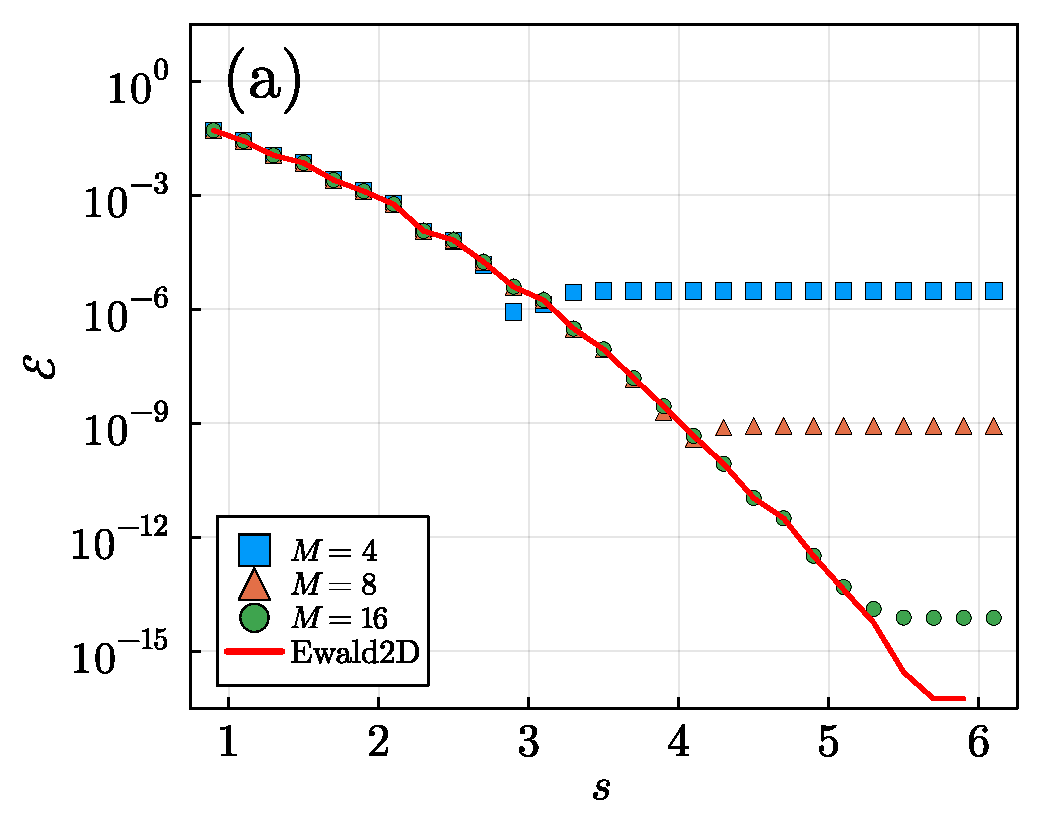
\includegraphics[width=0.48\textwidth]{figs/fig_error_fixn.pdf}
	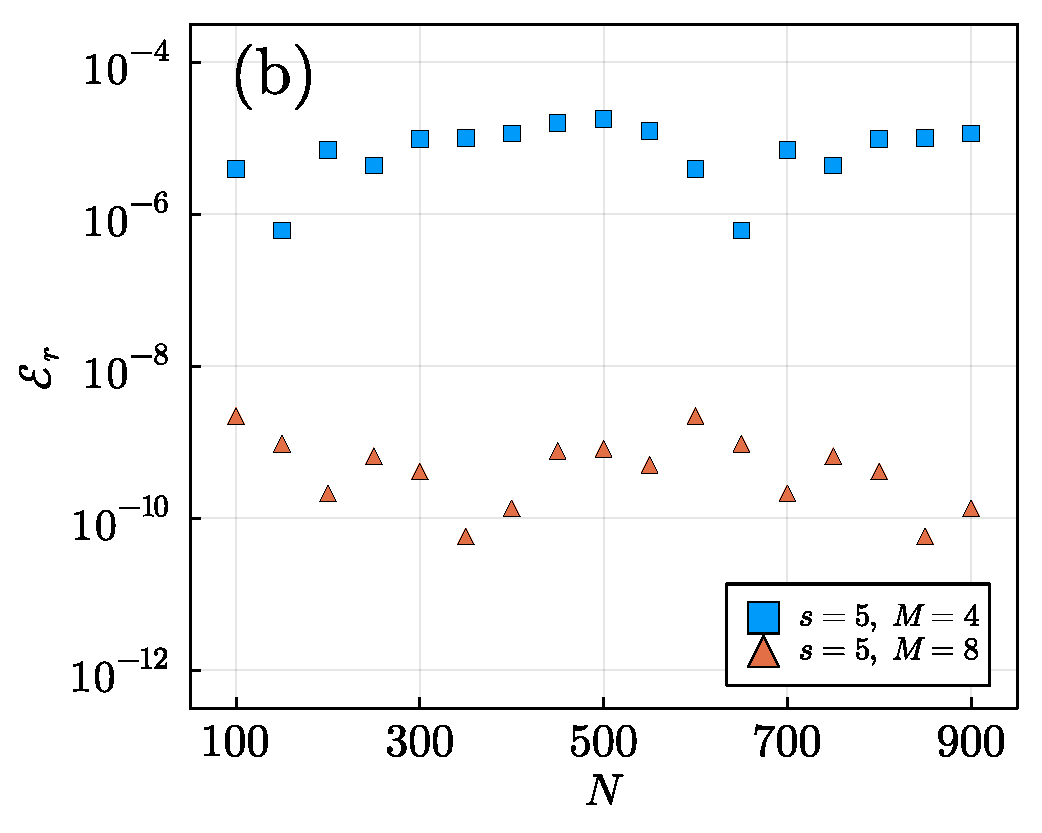
\includegraphics[width=0.48\textwidth]{figs/fig_error_N.pdf}
	\caption{
		Accuracy in the electrostatic energy by the SOEwald2D method. (a): absolute error as a function of $s$; (b): relative error as a function of total number of ions $N$ with fixed ion density $\rho_{s}$. Results with different number of exponentials $M$ are considered. 
	}
	\label{fig:error_fixn}
\end{figure}

\begin{figure}[ht]
	\centering
	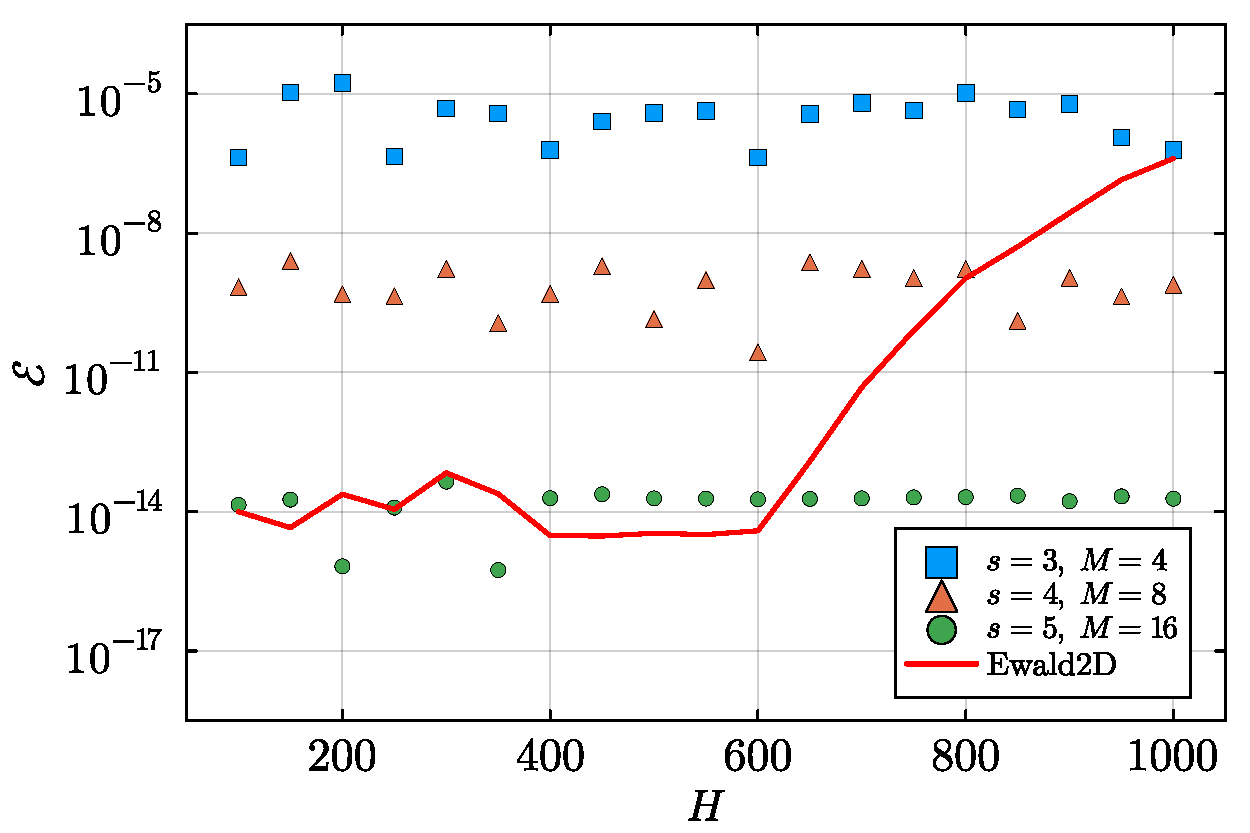
\includegraphics[width=0.6\textwidth]{figs/fig_error_Lz.pdf} 
	\caption{
		The absolute error in electrostatic energy is evaluated for the SOEwald2D method using three sets of parameters, as well as for the Ewald2D method with $s=5$, as a function of the system's thickness $H$. 
		% The system consists of $100$ uniformly distributed particles, with dimensions $L_x=L_y=100$ along the periodic dimensions. The Ewald parameter is set to $\alpha = 0.1$.
	}
	\label{fig:error_Lz}
\end{figure}

As discussed at the end of Section~\ref{sec::ewald2d}, one notable drawback of the original Ewald2D method is the occurrence of catastrophic error cancellation when the size of the non-periodic dimension increases. 
To quantify this effect, one shall study the absolute error in electrostatic energy as a function of $H$. 
The Ewald2D truncation parameter~$s= 3, 4, 5$ are chosen for~$M = 4, 8, 16$, respectively, to obtain optimal accuracy as is guided by Figure~\ref{fig:error_fixn} (a).
The system consists of $100$ uniformly distributed particles, with dimensions $L_x = L_y = 100$ along the periodic dimensions, and the Ewald parameter is set to be $\alpha = 0.1$.
A double-precision floating-point (FP64) arithmetic for both the Ewald2D and SOEwald2D methods is employed, while the reference solution is obtained using the Ewald2D with a quadruple-precision floating-point (FP128) arithmetic, ensuring a sufficient number of significant digits. 
The results presented in Figure~\ref{fig:error_Lz} clearly illustrate that the error of the Ewald2D method increases rapidly with $H$.
In contrast, the error of the SOEwald2D method remains independent of $H$ for various values of $s$ and $M$, thanks to its stable and well-conditioned summation procedure.

For many existing methods, the accurate evaluation of the forces exert on particles can be strongly influenced by the particle's location in~$z$. 
Due to the uniform convergence of SOE approximation, our method does not suffer from this issue, which is illustrated by two commonly employed examples that have been extensively studied in literature~\cite{lindbo2012fast,de2002electrostatics}. 
In the first example, one considers a system consisting of $50$ anions and $50$ cations arranged in a cubic geometry with a side length of $100$, along with neutral slabs.  
The pointwise error of the force, represented as $\sqrt{\mathscr{E}_{x}^2+\mathscr{E}_{y}^2+\mathscr{E}_{z}^2}$,  is calculated as a function of the particles' $z$-coordinates. 
This evaluation is conducted for various $(s,M)$ pairs, with the Ewald splitting parameter $\alpha=0.1$. 
Figure~\ref{fig:error_ef}(a) clearly demonstrates that the pointwise error in force is independent with its relative position in $z$. 
In the second example, one considers a system of the same size but with two non-neutral slabs. 
The surface charge densities are set as $\sigma_{\mathrm{top}} = \sigma_{\mathrm{bot}} = -0.005$, and the system contains $100$ monovalent cations such that the neutrality condition Eq.~\eqref{eq::chargeneu} is satisfied. 
Figure~\ref{fig:error_ef}(b) indicates that for such non-neutral slabs case, the pointwise error in forces calculated by the SOEwald2D method remains independent with $z$.

\begin{figure}[ht]
	\centering
	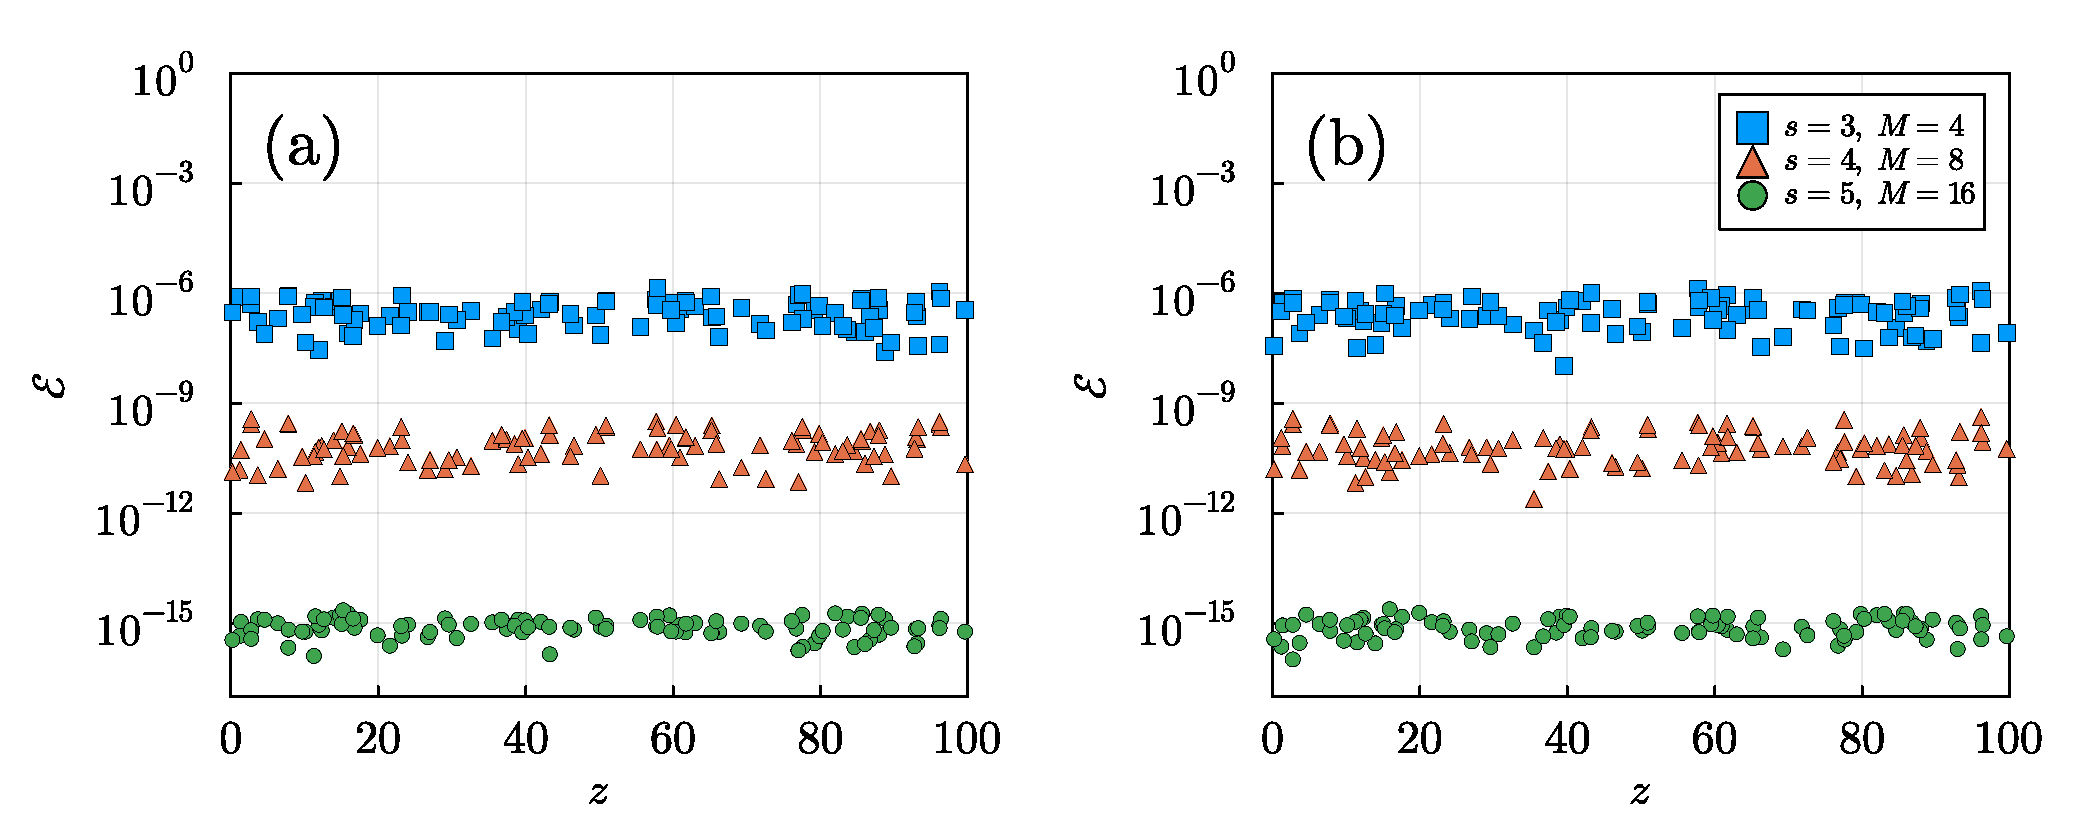
\includegraphics[width=\textwidth]{figs/fig_error_ef.pdf} 
	\caption{
		The absolute error in the pointwise electrostatic forces calculated using the SOEwald2D versus particles' $z$-coordinates. 
		Two different scenarios are considered: (a) uniformly distributed 50 anions and 50 cations and (b) uniformly distributed 100 cations with surface charge densities $\sigma_{\mathrm{top}}= \sigma_{\mathrm{bot}} = -0.005$.
	}\label{fig:error_ef}
\end{figure}

\subsection{Accuracy of the RBSE2D method}\label{subsec::RBSE2D}

In contrast to the deterministic SOEwald2D and Ewald2D methods, the  RBSE2D employs unbiased stochastic approximations and its convergence should be investigated in the sense of ensemble averages, as has been carefully discussed in Sec.~\ref{sec:rbm}. 
%The intuition why such stochastic methods work is that the effect of random approximations accumulates in time. Since the random approximation is unbiased, the random errors will roughly cancel out over time. This ``law of large numbers'' type mechanism in time then makes the random method work. 
Therefore, we conduct a series of MD simulations to validate the accuracy of the ensemble averaged equilibrium and dynamical quantities such as particles' concentrations and  mean-squared displacements (MSD) computed using the RBSE2D algorithm.

\begin{figure}[ht]
	\centering
	\begin{minipage}[c]{\textwidth}
		\centering
		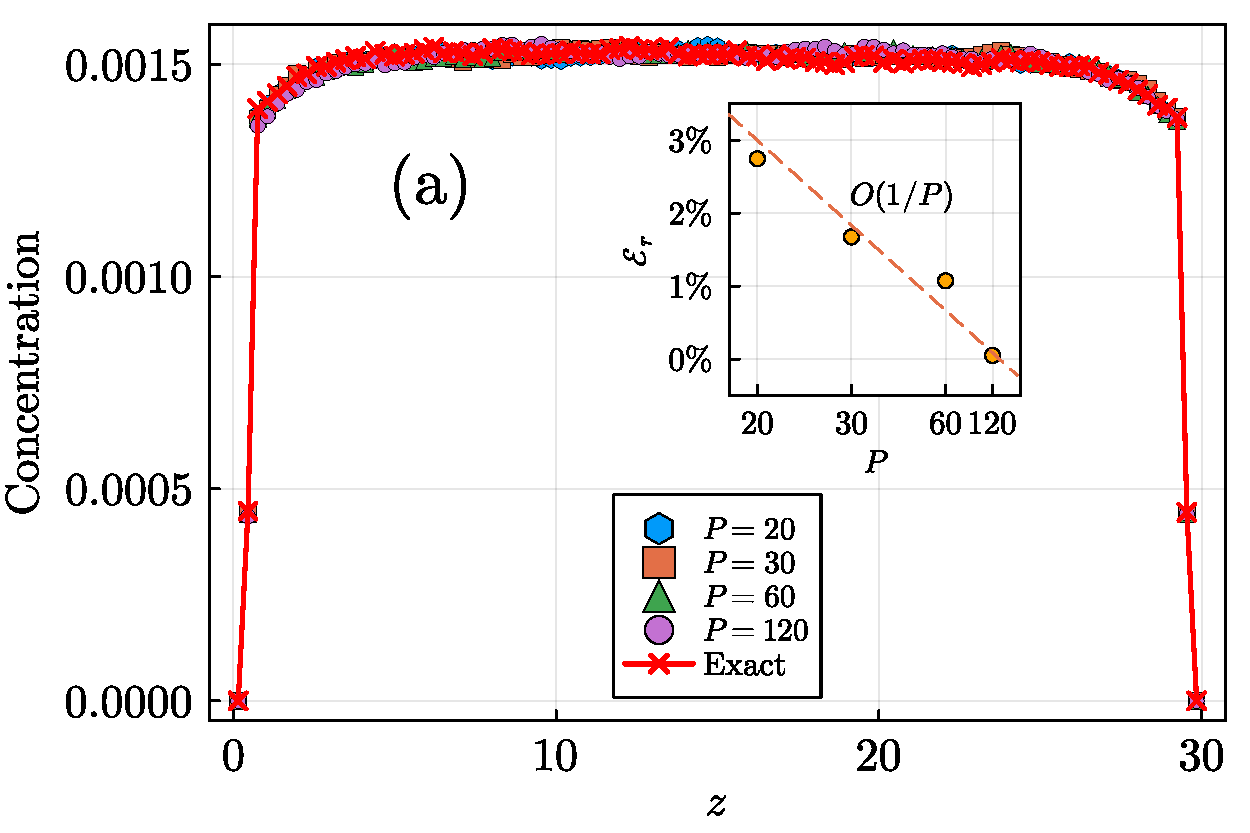
\includegraphics[width=0.6\textwidth]{figs/hist_norm.pdf}
		\label{fig:compare}
	\end{minipage} \\
	\begin{minipage}[c]{\textwidth}
		\centering
		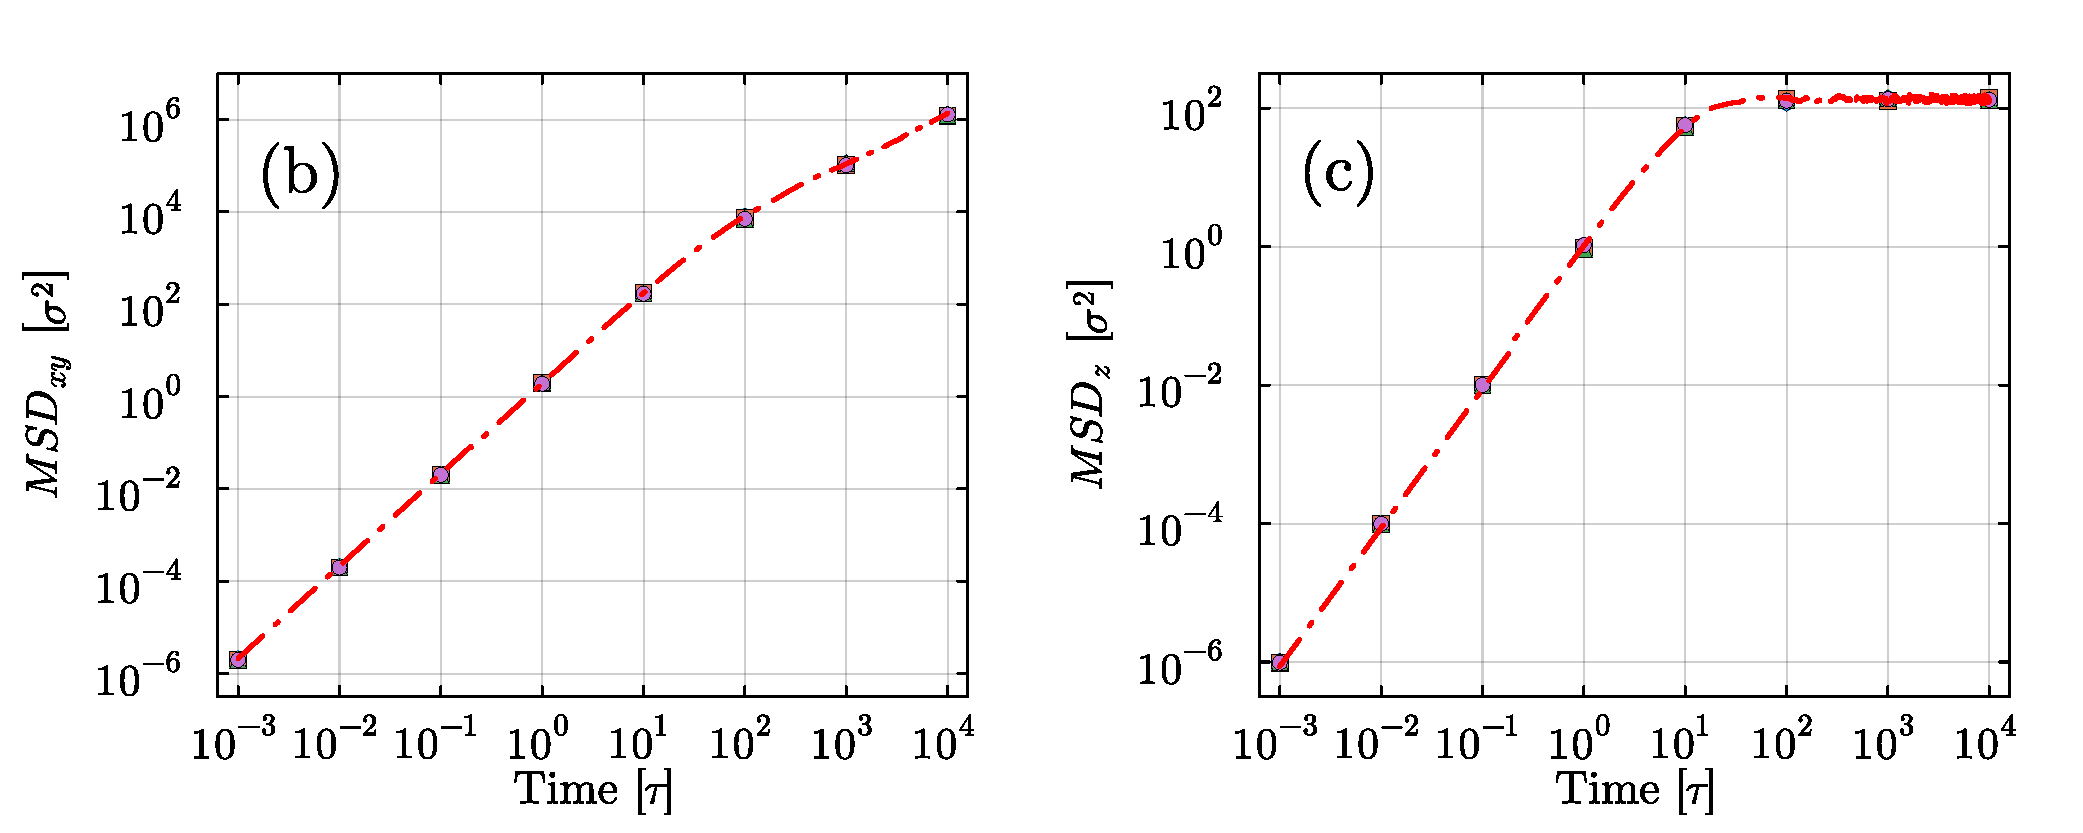
\includegraphics[width=\textwidth]{figs/msd_norm.pdf} 
		\label{fig:msd_norm}
	\end{minipage} 
	\caption{
		(a) The concentration of cations along $z$, with subplot indicating the convergence in the relative error of the average electrostatic energy as a function of batch size~$P$; (b) and (c) the MSD profiles in~$xy$ and~$z$ against time for a $1:1$ electrolyte confined by neutral slabs. 
		Results by using different batch sizes $P=20, 30, 60, 120$ are shown. 
	}
	\label{fig:norm}
\end{figure}

The first benchmark example is a coarse-grained MD simulation of  $1:1$ electrolytes in the NVT ensemble. 
Following the primitive model~\cite{frenkel2023understanding}, ions are represented as soft spheres with diameter $\sigma$ and mass $m$, interacting through the Coulomb potential and a purely repulsive shifted-truncated Lennard Jones (LJ) potential. 
The LJ potential is given by
\begin{equation}
	U_{\text{LJ}}(r) = 
	\begin{cases}
		4 \epsilon \left[ \left(\dfrac{\sigma}{r}\right)^{12}-\left(\dfrac{\sigma}{r}\right)^6 + \dfrac{1}{4}\right],\quad & r < r_{\text{LJ}}, \\
		0, & r \geq r_{\text{LJ}},
	\end{cases}
\end{equation}
where $r_{\text{LJ}} = 2^{1/6} \sigma$ is the LJ cutoff, $\epsilon = k_B T$ is the coupling strength, $k_B$ is the Boltzmann constant, and $T$ is the external temperature. 
The simulation box has dimensions $L_x = L_y = 100 \sigma$ and $H = 30 \sigma$, where the ions confined within the central region by purely repulsive LJ walls located at $z = 0$ and $z = 30 \sigma$ with $\epsilon_{\text{wall}} = \epsilon_{\text{LJ}}$ and $\sigma_{\text{wall}} = 0.5 \sigma$. 
The system contains $218$ cations and anions, and both two walls are neutral. 
The simulation is performed with the time step~$\Delta=0.001\tau$, where~$\tau = \sqrt{m \sigma^2 / \eps_{\text{LJ}}}$ denotes the LJ unit of time. 
The temperature is maintained by using a Nos\'e-Hoover thermostat~\cite{frenkel2023understanding} with relaxation times $0.1\tau$, fluctuating near the reduce external temperature $T=1$.
The system is first equilibrated for~$5 \times 10^5$ steps, and the production phase lasts another~$1 \times 10^7$ steps. 
The configurations are recorded every $100$ steps for statistics. Results produced by the SOEwald2D method with parameters $\alpha=0.1$, $s=4$, and $M=8$ serve as the reference solution, where $\varepsilon\sim 10^{-8}$.

The ion concentration along the $z$-direction is measured, and presented in Figure~\ref{fig:norm}. 
For the RBSE2D method, simulations with varying batch sizes $P$ are performed, while keeping other parameters fixed at $\alpha = 0.3$, $s=4$, and $M=8$. 
It is observed that the results for all choices of $P$ are in excellent agreement with those obtained using the accurate SOEwald2D method. 
Furthermore, one evaluates the MSDs along both the periodic dimensions (Figure~\ref{fig:norm}(a)) and the non-periodic dimension (Figure~\ref{fig:norm}(b)), which describe the particles' anisotropic dynamic properties across a wide range of time scales. 
The RBSE2D methods for all $P$ yield almost identical MSD results as the SOEwald2D method. 
The confinement effect in $z$ leads to a $MSD_z$ profile that clearly indicates a subdiffusion, while $MSD_{xy}$ exhibits a normal diffusion process. 
Clearly, the RBSE2D method successfully captures this anisotropic collective phenomenon.


\begin{figure}[ht]
	\centering
	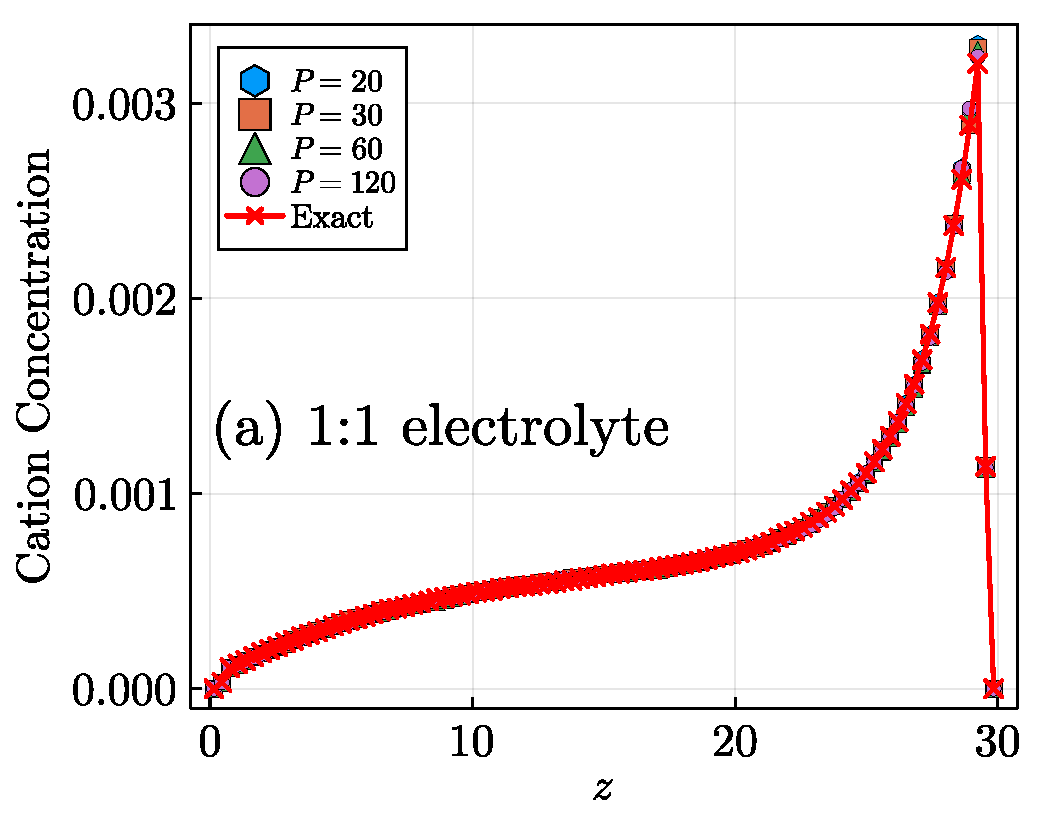
\includegraphics[width=0.49\textwidth]{figs/hist_Ez.pdf} 
	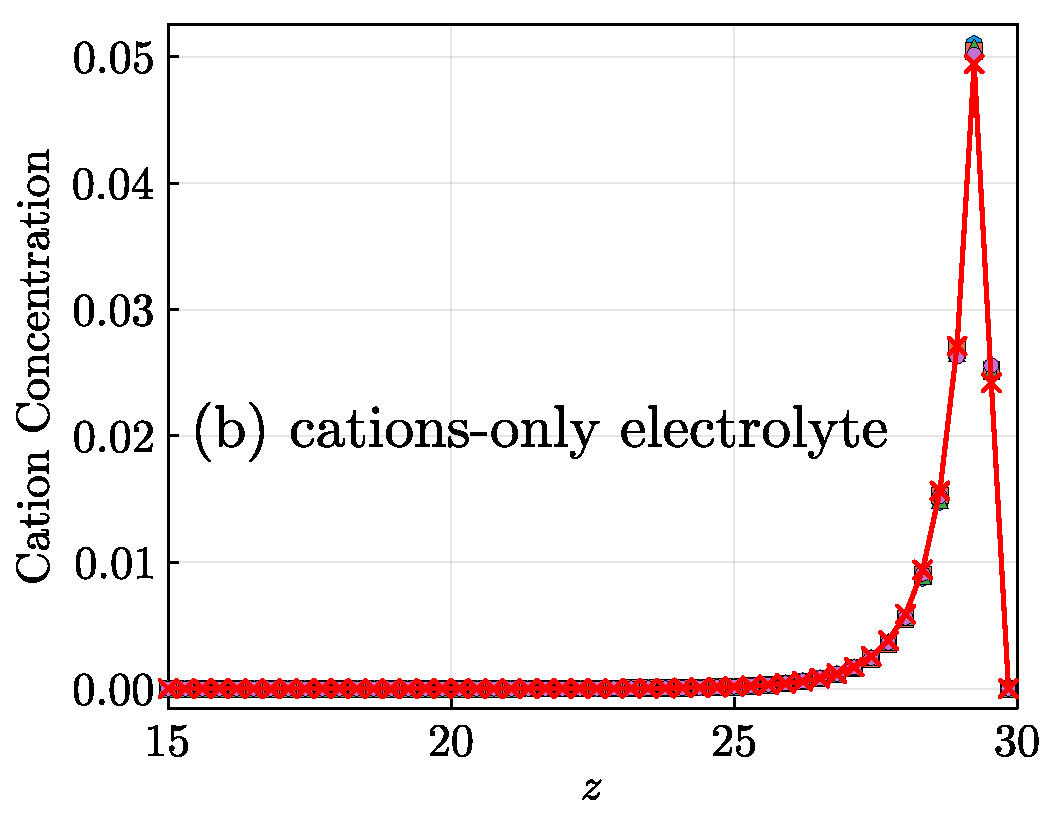
\includegraphics[width=0.49\textwidth]{figs/hist_cation.pdf}
	\caption{
		Concentration of cations in $z$ for (a) a $1:1$ electrolyte confined between two charged slabs and (b) a cations-only system confined between two slabs, one of which is charged to neutralize the system. 
	}
	\label{fig:Ez_density}
\end{figure}


To assess the performance of our RBSE2D method for systems with non-neutral slabs, one studies
a $1:1$ electrolyte containing~$218$ anions and~$218$ cations with~$q = \pm 1$, and with surface charge densities $\sigma_{\mathrm{bot}}=0.0218$ and~$\sigma_{\mathrm{top}}=-0.0218$. The simulation box is set to be $L_x = L_y = 100 \sigma$ and $H = 30 \sigma$.
The resulting equilibrium concentration of cations is shown in Figure~\ref{fig:Ez_density}(a), indicating that results of RBSE2D method with different batch sizes are in good agreement with that of the reference SOEwald2D method. 
% The subplot of Figure~\ref{fig:Ez_density}(a) also depicts the convergence as the batch size $P$ increases, which is consistent with our analysis.

We further investigate the most challenging scenario for a system with free cations only, which are confined by non-neutral slabs, so that boundary layers can form at the vicinity of the slabs. 
In particular, the system consists of $436$ monovalent cations and is confined by slabs with surface charge densities $\sigma_{\mathrm{bot}}=0$ and $\sigma_{\mathrm{top}}=-0.0436$ to ensure overall charge neutrality. The concentration of free ions is depicted in Figure~\ref{fig:Ez_density}(b), exhibiting excellent agreement with the results obtained using the SOEwald2D method. 
% The subplot in Figure~\ref{fig:Ez_density}(b) also demonstrates the expected convergence of the RBSE2D method as the batch size increases. 
These findings indicate that choosing a small batch size $P\sim O(1)$ is sufficient for generating accurate MD results by using the RBSE2D method.

\subsection{CPU performance}
The CPU performance comparisons among the SOEwald2D, RBSE2D, and the original Ewald2D methods are conducted for MD simulations of $1:1$ electrolyte systems with varying system sizes. 
All calculations are performed on a Linux system equipped with an Intel Xeon Platinum 8358 CPU (2.6 GHz, 1 single core); and by using a self-developed package developed in Julia language. 
To ensure a fair comparison, we maintain the same accuracy across all methods. We fix $s=4$ and set $M=8$ for the SOE approximation, resulting in errors at~$\sim10^{-8}$ for both the Ewald2D and SoEwald2D methods. %as shown in Figure~\ref{fig:error_fixn}(a).
Subsequently, we set the batch size as $P=120$ for the RBSE2D method, with which the RBSE2D-based MD simulations achieve the same accuracy as the SOEwald2D method, as has been illustrated in the previous results.
%It is remarked that the Ewald2D, SOEwald2D, and RBSE2D methods scale as $O(s^2)$, $O(s^2 M)$, and $O(s^2 M P)$, respectively.
Finally, for each of the methods, the Ewald splitting parameter $\alpha$ is always adjusted to achieve optimal efficiency.
The CPU time comparison results are summarized in Figure~\ref{fig:times_compare}. 
It is evident that the CPU cost of the Ewald2D, SOEwald2D, and RBSE2D methods scale as $O(N^2)$, $O(N^{7/5})$, and $O(N)$, respectively, which is consistent with our complexity analysis. 
Remarkably, the RBSE2D method demonstrates a significant speedup of $3\times 10^3$-fold compared to the Ewald2D for a system with $N=10^{4}$ particles, enabling large-scale MD simulations on a single core.

An additional observation is regarding the memory consumption and data input/output (I/O) on the maximum system size that can be simulated using the same computational resources. 
In Figure~\ref{fig:times_compare}, it is demonstrated that when utilizing a single CPU core, the Ewald2D and SOEwald2D methods are limited to simulating system sizes of up to about $3 \times 10^4$ and $3 \times 10^5$ particles, respectively. 
In contrast, the RBSOEwald method can handle systems containing about $5 \times 10^6$ particles. 
This is attributed to the reduced number of interacting neighbors that need to be stored in the RBSE2D algorithm, allowing a much smaller real space cutoff $r_c$. 
This significant saving in memory consumption is achieved by the algorithm developed in this study, highlighting its potential as an effective algorithm framework for large-scale simulations of quasi-2D Coulomb systems.

\begin{figure}[ht]
	\centering
	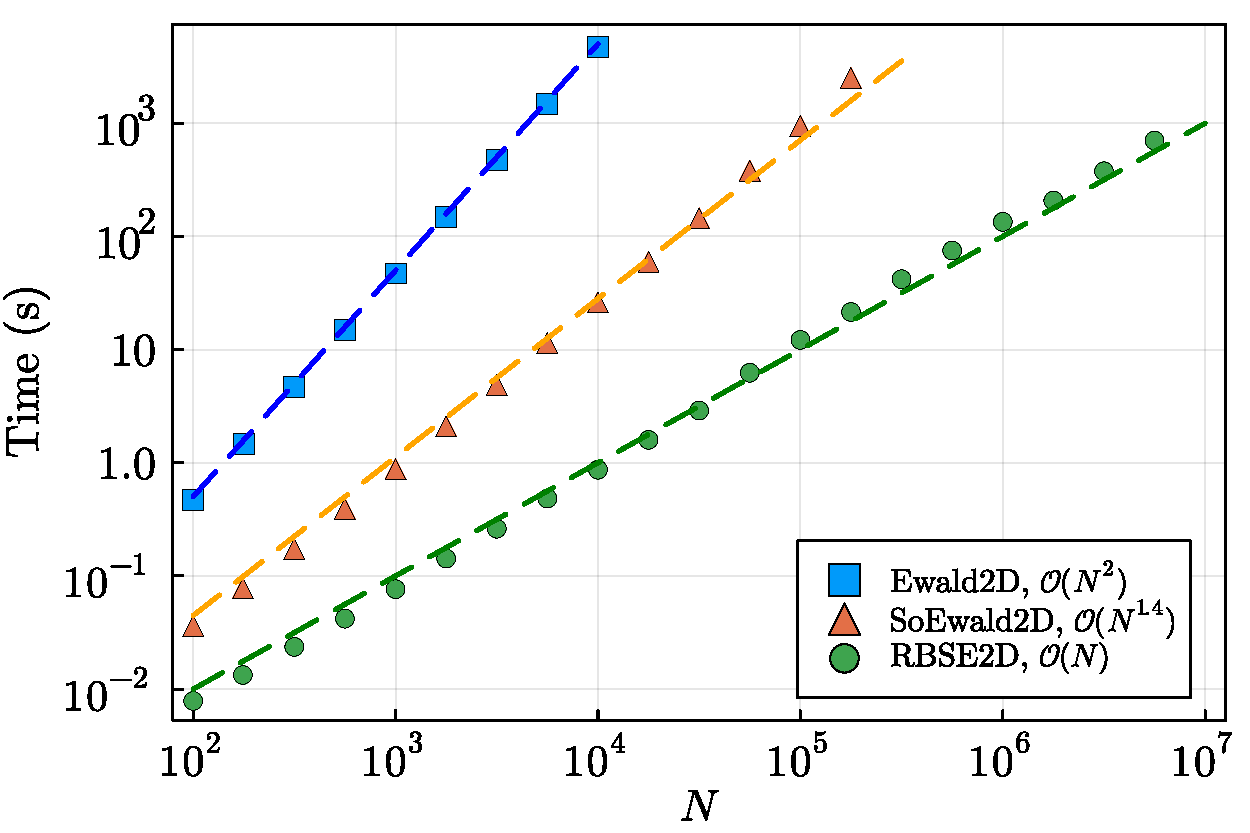
\includegraphics[width=0.6\textwidth]{figs/times_compare.pdf} 
	\caption{
		The CPU time cost for the Ewald2D, SOEwald2D, and RBSE2D methods versus the number of particles $N$, with fixed particle density $\rho_s$. 
	}
	\label{fig:times_compare}
\end{figure}
\newpage

\chapter{RBE2D for Dielectrically Confined Coulomb Systems}
\label{chp_rbe2d}
In Chapter~\ref{chp_soewald2d}, we introduced an efficient algorithm, the SOEwald2D method, to compute the electrostatic energy and force of a quasi-2D system in a homogeneous dielectric medium.
However, in most of the practical applications, the system is confined by dielectric interfaces, which is a more challenging problem.
In this chapter, we focus on the case of dielectrically confined Coulomb systems.
First, we derive the accurate error estimates for the Ewald summation for dielectrically confined Coulomb systems.
Then, we introduce the Random Batch Ewald2D (RBE2D) method, which is a fast and accurate method for computing the electrostatic energy and force of dielectrically confined Coulomb systems.

\section{Random batch Ewald2D method}\label{sec::RBE2D}

In this section, we introduce the random batch Ewald2D (RBE2D) method, which is a mesh-free fast algorithm for computing the electrostatic force in quasi-2D systems.
After reformulating the Ewald2D summation as a 3D one, we can directly apply the RBE method to accelerate the reciprocal-space sum and reaching an optimal $O(N)$ scaling.
The detailed algorithm is presented in Subsection~\ref{subsec::RBE2D_algorithm}.
We then prove the unbiasedness and variance of the RBE2D method in Subsection~\ref{subsec::convergence}.
Finally, we extend the RBE2D method to dielectric-confined systems in Subsection~\ref{subsec::IBCELCDielectric}.

\subsection{The algorithm}\label{subsec::RBE2D_algorithm}

As been introduced in Section~\ref{sec::icm_ewald2d}, the Ewald2D summation can be reformulated as a 3D one, and here we apply the RBE method to accelerate the reciprocal-space sum.
Instead of deterministically computing the $\V k$-space sum in Eq.~\eqref{eq::U3D_Four} either directly or via FFT, we now evaluate it through a stochastic approximation, namely, the random ``mini-batch'' sampling~\cite{jin2020random}. 
Notice that the low $\V k$ modes are more important due to the $e^{-k^2/(4\alpha^2)}$ factor, an importance sampling strategy was further developed for variance reduction.
% The random batch Ewald (RBE) method has recently been developed for fully periodic systems~\cite{jin2021random,liang2022superscalability, liang2023random}, and here we extend it to quasi-2D systems.

The long-range component of the electrostatic force exerts on $i$-th particle is given by $\V F_i^{\ell}=-\nabla_{\bm{r}_i}U_{\ell}$, its random batch approximation is denoted as
\begin{equation}\label{eq:forceRBE}
\begin{aligned}
    \V {\tilde{F}}_i^{\ell}=-\sum_{\eta=1}^P \frac{S}{P}\frac{4\pi q_i\V k_\eta}{Vk_\ell^2} \te{Im}\left(e^{-\i \V k_\eta\cdot \V r_i}\rho(\V k_\eta)\right)\;,
\end{aligned}
\end{equation}
where $P$ is the batch size, $V=L_xL_yL_z$ is the volume of the extended simulation domain $\Omega_{\text{3D}}$, 
 {
$\rho(\V{k})$ is the \textit{structure factor} defined as
\begin{equation}
    \rho(\V{k})=\sum_{j=1}^N q_j e^{\i \V k\cdot \V r_j}\;,
\end{equation}
}
and $S$ is the normalizing constant,
\begin{equation}\label{eq:normalizingS}
\begin{aligned}
S=\sum_{\V k \neq 0} e^{-k^2/(4\alpha^2)}\;.
\end{aligned}
\end{equation}
%Due to the high-dimensional separability of the Gaussian function, 
In MD simulations, it is convenient to employ the Metropolis algorithm~\cite{metropolis1953equation} to sample from $\mathscr{P}(\bm{k})=e^{-k^2/(4\alpha^2)}/S$. 
 {Our numerical experiments indicate that the average acceptance rate exceeds $90\%$, rendering the correlation between samples negligible. In practice, one can further introduce a downsampling factor $\mathcal{P}$, namely, select $1$ sample from every $\mathcal{P}$ sampling steps to further eliminate the correlation (we take $\mathcal{P}=5$ in our calculations, and the autocorrelation decays to approximately $10^{-3}$, which is already a very small value), and this downsampling factor does not compromise overall efficiency, as the cost of sampling procedure is relatively low. Note that alternative methods, such as directly sampling from discrete multivariate Gaussian distributions by truncating at certain $k_{\mathrm{max}}$, are also applicable.}

%It should be noted that, the Metropolis algorithm generated samples are auto-correlated, to further reduce the variance, we take $1$ sample out of every $5$ sampling steps, to ensure successive samples are uncorrelated.}
% {Additionally, the acceptance rate is very high (more than $80\%$), so that the computational cost for sampling is negligible.}
%rev{An alternative, and presumably more efficient sampling approach is to directly sample from $\mathscr{P}(\bm{k})$, which requires truncating the series summation~Eq.~\eqref{eq:normalizingS} at certain $k_{\mathrm{max}}$.}

For quasi-2D systems, the RBE2D method offers a particular advantage: it is mesh free, so that unlike existing grid-based fast algorithms, the computational cost is independent   {of the} added vacuum layer thickness. This statement is justified more rigorously in Theorem~\ref{Thm::1}. 
 {In the theorem, one utilizes the Debye-H\"uckel (DH) assumption for non-ideal electrolytes~\cite{levin2002electrostatic} (also see Appendix F in \cite{gan2024fast}), where the ensemble-averaged charge distributions around a charged particle follow the Boltzmann distribution.
}

\begin{thm}\label{Thm::1} 
    Denote the fluctuation of the random batch approximation in force by $\V \Xi_{\V F,i}=\V {\tilde{F}}_i^{\ell}-\V {F}_i^{\ell}$. The random variable $\V \Xi_{\V F,i}$ has zero expectation, i.e., $\mathbb{E}\V \Xi_{\V F,i}=\V 0$, and its variance is given by
    \begin{equation}\label{eq::30}
        \mathbb{E}|\V \Xi_{\V F,i}|^2=\frac{1}{P}\left[\frac{(4\pi q_i)^2S}{V^2}\sum_{\bm{k}\neq \bm{0}}\frac{e^{-k^2/(4\alpha^2)}}{k^2}\left|\emph{Im}\left(e^{-\i \V k \cdot \V r_i}\rho(\V k)\right)\right|^2-|\V F_{i}^{\ell}|^2\right]
    \end{equation}
    which is bounded and scales as $\mathcal O(1/P)$. Furthermore, under the DH assumption, $\mathbb{E}|\V \Xi_{\V F,i}|^2$ is independent of both the particle number $N$ and the size $L_z$.
\end{thm}

\begin{proof}%[Proof of \emph{Theorem}~\emph{\ref{Thm::1}}]
    The property of unbiasedness in Theorem~\ref{Thm::1} is straightforward and guarantees the consistency of the stochastic approximation, i.e., $\mathbb{E}\V{ \tilde{F}}_i^{\ell}=\mathbb{E}\V {F}_i^{\ell}$. 
    Let us now consider the variance.
    By the DH assumption, the structure factor term in Eq.~\eqref{eq::30} is bounded by a constant $C$~\cite{jin2021random} for $\bm{k}\neq \bm{0}$,
    \begin{equation}
        \left|\te{Im}\left(e^{-\i \V k\cdot \V r_i}\rho(\V k)\right)\right|^2\leq C,
    \end{equation}
    and vanishes for $\bm{k}=\bm{0}$. 
    Further by the monotonicity of Gaussian on $[0, +\infty )$, it follows that
    \begin{equation}\label{eq::32}
        \begin{split}
            \mathbb{E}|\V \Xi_{\V F,i}|^2\leq \frac{8 CSq_i^2}{PV}\int_{0}^{\infty}e^{-k^2/(4\alpha^2)}dk= \frac{8\sqrt{\pi}\alpha CSq_i^2}{PV}\;.%\mathbb{E}|\V \Xi_{\V F,i}|^2&\leq\frac{(4\pi q_i)^2CS}{PV^2}\sum_{\bm{k}\neq\bm{0}}\frac{e^{-k^2/(4\alpha^2)}}{k^2}\leq \frac{8 CSq_i^2}{PV}\int_{0}^{\infty}e^{-k^2/(4\alpha^2)}dk= \frac{8\sqrt{\pi}\alpha CSq_i^2}{PV}\;.
        \end{split}
    \end{equation}
    Analogously, one can obtain the following estimate for the normalization constant $S$:
    \begin{equation}\label{eq::Sa}
        \begin{split}
            S\leq \frac{V}{(2\pi)^3}\int_{0}^{\infty}4\pi k^2e^{-k^2/(4\alpha^2)}dk=\frac{\alpha^3V}{\pi^{3/2}}.
        \end{split}
    \end{equation}
    Substituting Eq.~\eqref{eq::Sa} into Eq.~\eqref{eq::32} yields
    \begin{equation}
        \mathbb{E}|\V \Xi_{\V F,i}|^2\leq\frac{8\alpha^4Cq_i^2}{\pi P}\sim \mathcal O\left(\frac{1}{P}\right)
    \end{equation}
    which is independent of either $N$ or $L_z$.
\end{proof}

Theorem~\ref{Thm::1} suggests that the variance in the random batch approximation can be effectively controlled %within the mean-field region 
by appropriately choosing the batch size $P$, which is independent   {of the} particle number $N$.
In the context of Ewald summation, typical choices for $\alpha$ are $(\sqrt{N}/V)^{1/3}$ for direct truncation~\cite{kolafa1992cutoff} and $(N/V)^{1/3}$ for FFT-based calculation~\cite{deserno1998mesh}. 
%For RBE2D, select $\alpha\sim \rho_{r}^{1/3}$, which ensures efficient real space computations and accelerated Fourier space computations. When the system becomes more dilute due to an increase in $L_z$ while keeping $N$ fixed, the upper bound of the variance decreases at a rate of $O(L_z^{-4/3})$. 
Now for the RBE2D method, it is clear that changing the vacuum layer thickness does not affect its efficiency. 
%However, the practical case may deviate from this ideal assumption due to the spatial anisotropy of the ion distribution, which is confined within the range of $[0,H]$. 
In practice, we set $\alpha\sim N^{1/3}/(L_xL_yH)^{1/3}$ (independent of $L_z$), then it is expected that the variance of the force remains at the same level as one changes $L_z$.
This is further validated by numerical results in Section~\ref{subsec::electrolyte-neutral}.

\subsection{Convergence and complexity of the RBE2D} \label{sec::convergence}

In this section, we further examine the convergence and complexity of RBE2D accelerated MD simulations. 
First, we revisit the the common purpose of MD simulations, which is to explore the configuration space and obtain static/dynamic ensemble-averaged properties by solving the equations of motion for $N$ interacting particles.
For example, consider the widely used canonical ensemble, where the system has fixed particle number $N$, volume $V$ and temperature $T$, which can be simulated as solving the following equations, namely, MD with Langevin thermostat~\cite{frenkel2023understanding}:
\begin{equation}\label{Langevin}
    \begin{aligned}
        & d \bm{r}_i=\bm{v}_i d t, \\
        & m_i d \bm{v}_i=\left[\bm{F}_i-\gamma \bm{v}_i\right] d t+\sqrt{2 \gamma k_{\mathrm{B}} T} d \bm{W}_i,
    \end{aligned}
\end{equation}
where $\bm{r}_i$, $m_i$, and $\bm{v}_i$ represent the position, mass, and velocity of the $i$-th particle, respectively. $\V{F}_i$ is the force exert {ed} on the $i$-th particle, $\{\bm{W}_i\}$ are i.i.d.~Wiener processes, and $\gamma$ is the reciprocal characteristic time scale associated with the thermostat.
In practice, the stochastic differential equations are discretized with proper numerical schemes and integrated with time step~$\Delta t$.
Let~$(\V{r}_i, \V{v}_i)$ be the solution to Eq.~\eqref{Langevin} with~$\bm{F}_i = \bm{F}^{\text{exact}}_i$, where~$\bm{F}^{\text{exact}}_i$ is the exact force on the $i$-th particle; and let $(\widetilde{\bm{r}}_i,\widetilde{\bm{v}}_i)$ be the solution to the same set of equations but with RBE2D approximated force given by~$\bm{F}_i = \bm{F}^{\text{exact}}_i + \bm{\Xi}_{\bm{F},i}$.
Then the relation between the two sets of solutions satisfies the following Theorem~\ref{thm::2}~\cite{jin2021convergence}.

\begin{thm}\label{thm::2}
If the forces $\bm{F}_i$ are bounded and Lipschitz, and the fluctuation of stochastic force satisfies $\mathbb{E}\V \Xi_{\V F,i}=0$, then for any $t_{\emph{MD}}>0$, there exists $C(t_{\emph{MD}})>0$ such that
\begin{equation}\label{eq::Convergence}
\sup _{t \in[0, t_{\emph{MD}}]} \sqrt{\frac{1}{N} \sum_{i=1}^N \mathbb{E}\left(\left|\bm{r}_i-\widetilde{\bm{r}}_i\right|^2+\left|\bm{v}_i-\widetilde{\bm{v}}_i\right|^2\right)} \leq C(t_{\emph{MD}}) \sqrt{\Lambda \Delta t}. %\sim C(t_{\emph{MD}}) \sqrt{\frac{\Delta t}{P}}.
\end{equation}
 {Here, $\Lambda$ is an upper bound for $\mathbb{E}|\V \Xi_{\V F,i}|^2$, and one has $\Lambda\sim \mathcal O(1/P)$ due to Theorem~\ref{Thm::1}.} 
\end{thm}

Theorem~\ref{thm::2} indicates that the RBE2D approximated dynamics is capable of capturing finite time structure and dynamic properties.
For long-time simulations, additional assumptions are needed regarding force regularity~\cite{jin2022random}. 
It   {is worth} noting that, although the Coulomb potential is neither bounded nor Lipschitz at $r=0$, actual MD simulations will include the Lennard-Jones (LJ) potential, which provides a  {strong repulsive force at short inter-particle distance and prevents the particles from getting too close. As a result, the singularities in both the Coulomb and LJ potentials will not be reached in practice as long as the time step is properly chosen, allowing to satisfy the condition of Theorem~\ref{thm::2}  for MD simulations.}

Additionally, following Theorem \ref{thm::2}, the fluctuations introduced by random batch approximation, $\V \Xi_{\V F,i}$,  can be physically understood as heating effects, which will cause a temperature drift for the system and is unwanted. 
For NVT and NPT ensembles, the heating effect can be eliminated by introducing appropriate thermostats such as the Langevin thermostat~\cite{feller1995constant}, the Nos\'e-Hoover (NH) thermostat~\cite{hoover1985canonical}, etc. With an additional weak-coupled bath on the Newtonian dynamics to avoid energy drift, the NVE ensemble can also be accurately simulated with random batch-type approximations~\cite{liang2024JCP}.

Next, we analyze the computational complexity of the RBE2D accelerated MD simulations. The detailed algorithm is summarized in Fig.~\ref{Alg::1}.  
In the RBE2D, the random batch importance sampling in Eq.~\eqref{eq:forceRBE} approximates the Fourier space force by summing over $P$ Fourier modes. 
At each step, $P$ structure factors, $\{\rho(\bm{k}_{\eta})\}_{\eta=1}^{P}$, are computed for all particles, resulting in a Fourier part complexity of $\mathcal{O}(PN)$. Furthermore, as shown in Theorems~\ref{Thm::1} and \ref{thm::2} and the analysis at the end of Section~\ref{subsec::RBE2D_algorithm}, the RBE2D error does not grow as $N$ or $L_z$ increases when the batch size $P=\mathcal{O}(1)$ and $\alpha\sim N^{1/3}/(L_xL_yH)^{1/3}$ are provided. 
The real space part of the RBE2D is short-ranged due to the rapid decay of factor $\erfc(\alpha r)$ and can be directly truncated by introducing a cutoff $r_c$. 
As a result, the real space complexity is proportional to the product of $N$ and the average number of neighbors within a volume of $4\pi r_c^3$ per particle. 
For a given truncation error tolerance, $r_c\sim \alpha^{-1}$, yielding a real space complexity $\sim \alpha^{-3}N/(L_xL_yH)=\mathcal{O}(1)$ per particle. 
As such, the total computational complexity is of $\mathcal{O}(N)$. 

\begin{algorithm}[ht]
 \caption{(RBE2D accelerated molecular dynamics for quasi-2D systems)}\label{Alg::1}
 \begin{algorithmic}[1]
  \State Choose $\alpha$, $r_c$ (the cutoff in real space), $\Delta t$, the vacuum layer parameter $L_z$, and batch size $P$. Initialize the positions and velocities of ions as well as surface charge densities. Set $N_T$ as the total MD time steps.
  \For {$n \text{ in } 1: N_T$}
  \State Sample $P$ nonzero frequencies $\bm{k}\sim e^{-k^2/(4\alpha)}$ by the Metropolis procedure to form  set $\mathcal{K}$.
  \State The $\V k$-space component of the force, $\bm{F}_i^{\ell}$, is computed using the random batch approximation $\widetilde{\V F}_i^{\ell}$ with the $P$ frequencies from the set $\mathcal{K}$.
  \State The real space component of the force, $\bm{F}_i^{s}$, is computed by the neighbor list method. %The rest force terms, including the YB correction $\V F_{i}^{\te{YB}}$, the renormalization term $\V F_{i}^{\te{renorm}}$, and the ion-wall force $\V F_{i}^{\te{wall}}$, can be directly computed.
  \State Integrate the equations of motion for time step $\Delta t$ with an appropriate thermostat and its corresponding integration scheme. %the total force
  %$$\V F_i=\widetilde{\V F}_i^{\ell}+\bm{F}_i^{\te{real}}+\V F_{i}^{\te{YB}} + \V F_{i}^{\te{wall}}$$
  
  \EndFor
 \end{algorithmic}
\end{algorithm}
Besides its linear complexity, the RBE2D method offers two other significant advantages:
\begin{itemize}
    \item  {Communication efficiency: The RBE2D method is embarrassingly parallel, requiring only a single global reduction of the structure factors for all $\mathcal{O}(P)$ samples when calculating the force using Eq.~\eqref{eq:forceRBE}.} This streamlined communication facilitates high scalability. 

    \item Vacuum layer flexibility: the RBE2D is mesh free, and choosing a larger vacuum layer thickness incurs no extra cost. This provides flexibility for one to always choose a proper $L_z$ to guarantee accuracy, without sacrificing efficiency.
\end{itemize}

\subsection{RBE2D method for dielectrically confined quasi-2D systems} \label{subsec::IBCELCDielectric}

We now extend the RBE2D method for efficient MD simulations of dielectrically confined quasi-2D Coulomb systems. 
First, given tolerance $\varepsilon$, one shall choose appropriate values for $M$ and $L_z$, such that the image series truncation error, the ELC term, and remainder error term can all be neglected. Then, let $\bm{F}_{\ell}^{\text{c}}$ denotes the $\V k$-space component of force acting on the $i$-th particle, it reads
\begin{equation}\label{eq::52}
\bm{F}_{\ell}^{\text{c}}(\bm{r}_i)=-\frac{2\pi}{L_xL_yL_z}\sum_{\bm{k}}{}^{\prime}\frac{e^{-\frac{k^2}{4\alpha^2}}}{k^2}\nabla_{\bm{r}_i}\left[\rho_{\bm{k}}\bar{\rho}_{\bm{k}}^{M}\right]+\bm{F}_{\text{IBC}}^{M}(\bm{r}_i)\;,%+\bm{F}_{\text{ELC}}^{M}(\bm{r}_i)+\bm{F}_{\text{err}}^{M}(\bm{r}_i)\;,
\end{equation}
where 
\begin{equation}\label{eq::rhorhoM}
\begin{split}
\nabla_{\bm{r}_i}\left[\rho_{\bm{k}}\bar{\rho}_{\bm{k}}^{M}\right]=&q_i\bm{k}\text{Im}\left[e^{-\i\bm{k}\cdot\bm{r}_i}\left(\rho_{\bm{k}}+\rho_{\bm{k}}^{M}\right)+\sum_{\substack{l=1\\ \text{even}}}^{M}\left(\gamma_{+}^{(l)}e^{-\i\bm{k}\cdot\bm{r}_{i+}^{(l)}}+\gamma_{-}^{(l)}e^{-\i\bm{k}\cdot\bm{r}_{i-}^{(l)}}\right)\rho_{\bm{k}}\right]\\
+&q_i\widehat{\bm{k}}\text{Im}\left[\sum_{\substack{l=1\\ \text{odd}}}^{M}\left(\gamma_{+}^{(l)}e^{-\i\bm{k}\cdot\bm{r}_{i+}^{(l)}}+\gamma_{-}^{(l)}e^{-\i\bm{k}\cdot\bm{r}_{i-}^{(l)}}\right)\rho_{\bm{k}}\right]
\end{split}
\end{equation}
with $\rho_{\bm{k}}^{M}$ the conjugate of $\bar{\rho}_{\bm{k}}^{M}$ and $\widehat{\bm{k}}=(k_x,k_y,-k_z)$. The calculation of Eq.~\eqref{eq::52} can also be accelerated via FFT, namely, the ICM-PPPM method~\cite{yuan2021particle}. 
If the image reflection level is truncated at $M$, the computational cost of ICM-PPPM is $\mathcal O(MN \log(MN))$. Thus for strongly confined systems, the cost of FFT-based method will increase rapidly as $M$ increases.
%This means that the cost does not increase rapidly as $M$ increases, which indicates that RBE2D is more suitable for systems with strong surface polarization. 
%The detailed formula is given in Eq.~\eqref{eq::F_c_Four_detail}.

We now again apply the importance sampling technique to approximate $\bm{F}_{\ell}^{\text{c}}$, yielding the following stochastic estimator as 
%More precisely, we regard the factor $e^{-\frac{k^{2}}{4\alpha^2}}$ as a discrete Gaussian distribution, and denote the resulting estimator of force as
\begin{equation}\label{eq::important}
\bm{F}_{\ell}^{\text{c}}(\bm{r}_i)\approx \bm{F}_{\ell}^{\text{c},*}(\bm{r}_i)=-\frac{2\pi }{L_xL_yL_z}\sum_{\eta=1}^{P}\frac{S}{P}\frac{\nabla_{\bm{r}_i}\left[\rho_{\bm{k}_{\eta}}\bar{\rho}_{\bm{k}_{\eta}}^{M}\right]}{k_{\ell}^2}+\bm{F}_{\text{IBC}}^{M}(\bm{r}_i),
\end{equation}
where $\{\bm{k}_{\eta}\}_{\eta=1}^{P}$ are the $P$ batches of wave vectors sampled from $\mathscr{P}(\bm{k})$. 
It is important to note that when surface charges are present at the interfaces~\cite{spohr1997effect,yi2017note,yuan2021particle}, a straightforward modification to Eq.~\eqref{eq::important} is required, which allows for the simultaneous treatment of discrete ions and continuous surface charges.
Detailed information can be found in the SM, Section S1.
And the real space component of force is given by Eq.~(SM1.3), which can still be evaluated by neighbor lists algorithms.

%The real space part of force, as given by Eq.~(SM1.3) in the SM, is computed via directly truncating at a cutoff radius $r_c$.
%In contrast to the fully periodic case, the choice of $r_c$ does not need to satisfy the minimum image principle along the $z$-direction. 
%For systems where $H\ll\min\{L_x,L_y\}$, selecting a larger $r_c$ can reduce the computational cost of the reciprocal space summation, but enlarges the number of included images as well, resulting in a decrease in efficiency.
%Hence, it is crucial to carefully calibrate $r_c$ with other parameters. 

Next, we describe a simple strategy for efficiently summing over the $2MN$ image charges.
% To reduce this cost, we present a more efficient approach. 
Notice that Eq.~\eqref{eq::rhorhoM} can be rewritten as
\begin{equation}\label{eq::56}
\begin{split}
    \nabla_{\bm{r}_i}\left[\rho_{\bm{k}}\bar{\rho}_{\bm{k}}^{M}\right]
    = & q_i\bm{k}\text{Im}\left[e^{-\i \bm{k}\cdot \bm{r}_i}\sum_{j=1}^{N}q_je^{\i\bm{k}\cdot\bm{r}_{j}}\left(1+e^{-2\i k_zz_j}Y_{\text{odd}}(k_z)+Y_{\text{even}}(k_z)\right)\right]\\
    + & q_i\bm{k}\text{Im}\left[e^{-\i \bm{k}\cdot\bm{r}_i}\left(1+e^{2\i k_zz_i}\overline{Y}_{\text{odd}}(k_z)\right)\rho_{\bm{k}}\right]+q_{i}\widehat{\bm{k}}\text{Im}\left[e^{-\i\bm{k}\cdot\bm{r}_i}\overline{Y}_{\text{even}}(k_z)\rho_{\bm{k}}\right],
\end{split}
\end{equation}
 {where the coefficients $Y_{\text{odd}}$ and $Y_{\text{even}}$ are defined as follows: 
\begin{equation}
    \begin{split}
        Y_{\text{odd}}(k_z) &= \sum_{\substack{l=1, \text{odd}}}^{M}\left[\gamma_{+}^{(l)}e^{\i k_z(l+1) H}+\gamma_{-}^{(l)}e^{-\i k_z (l-1)H}\right], \\ 
        Y_{\text{even}}(k_z) &= \sum_{\substack{l=1, \text{even}}}^{M}\left[\gamma_{+}^{(l)}e^{\i k_zl H}+\gamma_{-}^{(l)}e^{-\i k_z l H}\right].
    \end{split}
\end{equation}
This formulation enables the decoupling of the summation over particles index $j$ and their image index $l$. 
In practical simulations, one shall first precompute $Y_{\text{odd}}(k_z)$ and $Y_{\text{even}}(k_z)$ for each $\bm{k} \in \{\bm{k}_{\eta}\}_{\eta=1}^{P}$, as these are configuration independent, with a computational cost of $\mathcal{O}(PM)$. 
Subsequently, for a given particle configuration, one evaluates $\rho_{\bm{k}}$, along with the conjugates of $Y_{\text{odd}}$ and $Y_{\text{even}}$, and computes
\begin{equation}
    \sum_{j=1}^{N}q_je^{\i\bm{k}\cdot\bm{r}_{j}}\left(1+e^{-2\i k_zz_j}Y_{\text{odd}}(k_z)+Y_{\text{even}}(k_z)\right)
\end{equation}
for every $\bm{k}\in\{\bm{k}_{\eta}\}_{\eta=1}^{P}$, which incurs a cost of $\mathcal{O}(PN)$ operations. These intermediate variables are then utilized to evaluate $\nabla_{\bm{r}_i}\left[\rho_{\bm{k}}\bar{\rho}_{\bm{k}}^{M}\right]$ for all particles $i$ using Eq.~\eqref{eq::56}, adding another $\mathcal O(PN)$ to the cost. Finally, substituting the value of $\nabla_{\bm{r}_i}\left[\rho_{\bm{k}}\bar{\rho}_{\bm{k}}^{M}\right]$ into Eq.~\eqref{eq::important} allows for the computation of the first term on the right-hand side with $\mathcal{O}(PN)$ operations, followed by the addition of the IBC term, which incurs an $\mathcal{O}(N)$ cost. Consequently, the total computational cost for force evaluations is reduced from $\mathcal O(PMN)$ to $\mathcal O(P(M+N))$.
In practice, one shall still take $\alpha \sim N^{1/3}/(L_xL_yH)^{1/3}$ to ensure that the real space calculation costs $\mathcal{O}(N)$, then the $\V k$-space components of force can be calculated as such so that the complexity is reduced to $\mathcal{O}(P(M+N))$.}
Thus, the overall complexity of the RBE2D is approximately $\mathcal{O}(N)$ since both $P$ and $M$ are of $\mathcal O(1)$ and independent   {of} $N$.
The detailed algorithm for RBE2D accelerated MD in the presence of dielectric interfaces is summarized in Algorithm~\ref{alg::RBEalg}.

\begin{algorithm}[H]
 \caption{(RBE2D for quasi-2D systems under dielectric confinement)}\label{alg::RBEalg}
 \begin{algorithmic}[1]
  \State Choose $\alpha$, $r_c$ (the cutoff in real space), $\Delta t$, batch size $P$, image reflection level of truncation $M$, and the vacuum layer parameter $L_z$. Initialize the coefficients of dielectric jumps ($\varepsilon_{\rm{top}}$, $\varepsilon_{\rm{c}}$, $\varepsilon_{\rm{bot}}$) and the positions and velocities of charges $\bm{r}^0_i, \bm{v}^0_i$ for $1\le i\le N$. Set $N_T$ as the total MD time steps.
  %\State Sample sufficient number of nonzero $\bm{k}\sim e^{-k^2/(4\alpha)}$ by the MH procedure to form a set $\mathcal{K}$.
  \For {$n \text{ in } 1: N_T$}
  \State Sample $P$ nonzero frequencies $\bm{k}\sim e^{-k^2/(4\alpha)}$ by the Metropolis procedure to form set $\mathcal{K}$.
  \State The real space component of force is computed via a neighbor list algorithm (for both actual charges and image charges within $r_c$).
  \State The Fourier space component of  {the} force is computed via the random batch approximation $\bm{F}_{\ell}^{\text{c},*}$, with $P$ frequencies from the set $\mathcal{K}$.
  \State Integrate the equations of motions for time $\Delta t$ with  {an} appropriate integration scheme and some appropriate thermostat. 
  \EndFor
 \end{algorithmic}
\end{algorithm}

Finally, consider the fluctuation of random batch approximation of the force, denoted as $\bm{\Xi}_{\bm{F},i}^{\text{c}}=\bm{F}_{\ell}^{\text{c},*}(\bm{r}_i)-\bm{F}_{\ell}^{\text{c}}(\bm{r}_i)$, one can still show that 1) the variance of the RBE2D method is controlled via $\mathcal{O}(1/P)$ and is independent of $L_z$; 2) the RBE2D is capable to capture finite time structure and dynamic properties in MD simulations. 
The proof is similar to Theorems~\ref{Thm::1} and~\ref{thm::2}, and is thus omitted here.

\section{Numerical results}\label{sec::numerical}

In this section, numerical results are first presented for the homogeneous case, validating the performance of RBE2D accelerated MD simulations. 
Examples include coarse-grained models of electrolytes and all-atom SPC/E bulk water systems~\cite{berendsen1987missing} confined by two slabs without dielectric jumps, where all the quantities are defined and calculated in reduced LJ units and real units~\cite{frenkel2023understanding}, respectively.
Our method is implemented in LAMMPS (version 29Oct2020) \cite{thompson2021lammps} and performed on the ``Siyuan Mark-I'' high performance cluster at Shanghai Jiao Tong University. 
Each node is equipped with $2\times$ Intel Xeon ICX Platinum $8358$ CPU ($2.6$GHz, $32$ cores) and $512$ GB memory.
The code is highly optimized, where the message passing interface (MPI) and Intel AVX-512 instructions are used for parallelization and vectorization, respectively.

To benchmark the accuracy, several widely investigated quantities are computed, such as concentration, mean-squared displacement (MSD), velocity auto-correlation functions (VACF), ensemble-averaged energy distribution, etc. 
The calculation methods for these quantities are described in Section~\ref{Sec::phyquan}.
For comparison, we used the stable implementation of the PPPM2D method~\cite{crozier2001molecular} provided inside LAMMPS for systems without dielectric interfaces.
Results obtained using the PPPM2D method are labeled as ``PPPM''. 
For systems with dielectric interfaces, we used the HSMA method~\cite{liang2020harmonic} and the ICM-PPPM method~\cite{yuan2021particle}.
The parameters of the PPPM were automatically chosen in LAMMPS to achieve a desired relative error of $\Delta=10^{-4}$ for force evaluations~\cite{deserno1998mesh}. 
For the RBE2D, parameters such as $M$ and $L_z$ are selected according to Section~\ref{sec:parameter}; while
for the HSMA and ICM-PPPM, we use the same parameters suggested by Refs.~\cite{liang2020harmonic} and~\cite{yuan2021particle}, respectively. For all methods, the threshold in relative errors is set to $10^{-4}$.
To allow a fair comparison, the Ewald splitting parameter $\alpha$ is always set to be the same for RBE2D and PPPM methods.



\subsection{3:1 electrolytes immersed in an implicit solvent}\label{subsec::electrolyte-neutral}

We first perform coarse-grained MD simulations of $3:1$ electrolytes in the NVT ensemble. 
Following the primitive model, all the ions are represented as soft spheres of diameter $\sigma$ and mass $m$ that interact via  {electrostatic interactions} and a purely repulsive shifted-truncated LJ potential
\begin{equation}
	U_{\text{LJ}}=\begin{cases}
		4\varepsilon_{\text{LJ}}\left[\left(\dfrac{\sigma}{r_{ij}}\right)^{12}-\left(\dfrac{\sigma}{r_{ij}}\right)^6+\dfrac{1}{4}\right],~~~~r_{ij}\leq r_{\text{LJ}},\\
		0,~~~~r_{ij}>r_{\text{LJ}},	
	\end{cases}
\end{equation}
where $r_{ij}$ is the distance between $i$-th and $j$-th particles, $r_{\text{LJ}}=2^{1/6}\sigma$ the LJ truncation distance, $\varepsilon_{\text{LJ}}=k_{\text{B}}T$ the coupling strength, $k_{\text{B}}$ is the Boltzmann constant, and $T$ the temperature. These ions are immersed in a continuum solvent, characterized by a Bjerrum length 
$\ell_{\text{B}}=e^2/(4\pi \varepsilon_c k_{\text{B}}T)=3.5\sigma$. The system has dimensions $L_x=90\sigma$, $L_y=90\sigma$, and $H=30\sigma$, containing $750$ cations and $2250$ anions. The ions are confined in $z$ by purely repulsive LJ walls at $z=0$ and $z=30\sigma$, with parameters $\varepsilon_{\text{wall}}=\varepsilon_{\text{LJ}}$ and $\sigma_{i,\text{wall}}=0.5\sigma$. 
The initial $10^6$ steps with $\Delta t=10^{-3}\tau$ are performed for equilibrium, where $\tau=\sqrt{m\sigma^2/\varepsilon_{\text{LJ}}}$ denotes the LJ unit of time. The production phase follows for another $10^7$ steps, and the configurations are sampled every $100$ time steps for statistics. 
The temperature is maintained by using a Nos\'e-Hoover thermostat~\cite{hoover1985canonical} with relaxation times $0.01\tau$, %fluctuating near the reduce external temperature $T=1$. 
and $r_c$ is set as $10\sigma$ for both the RBE2D and PPPM methods.  

\begin{figure}[!ht]
	\centering
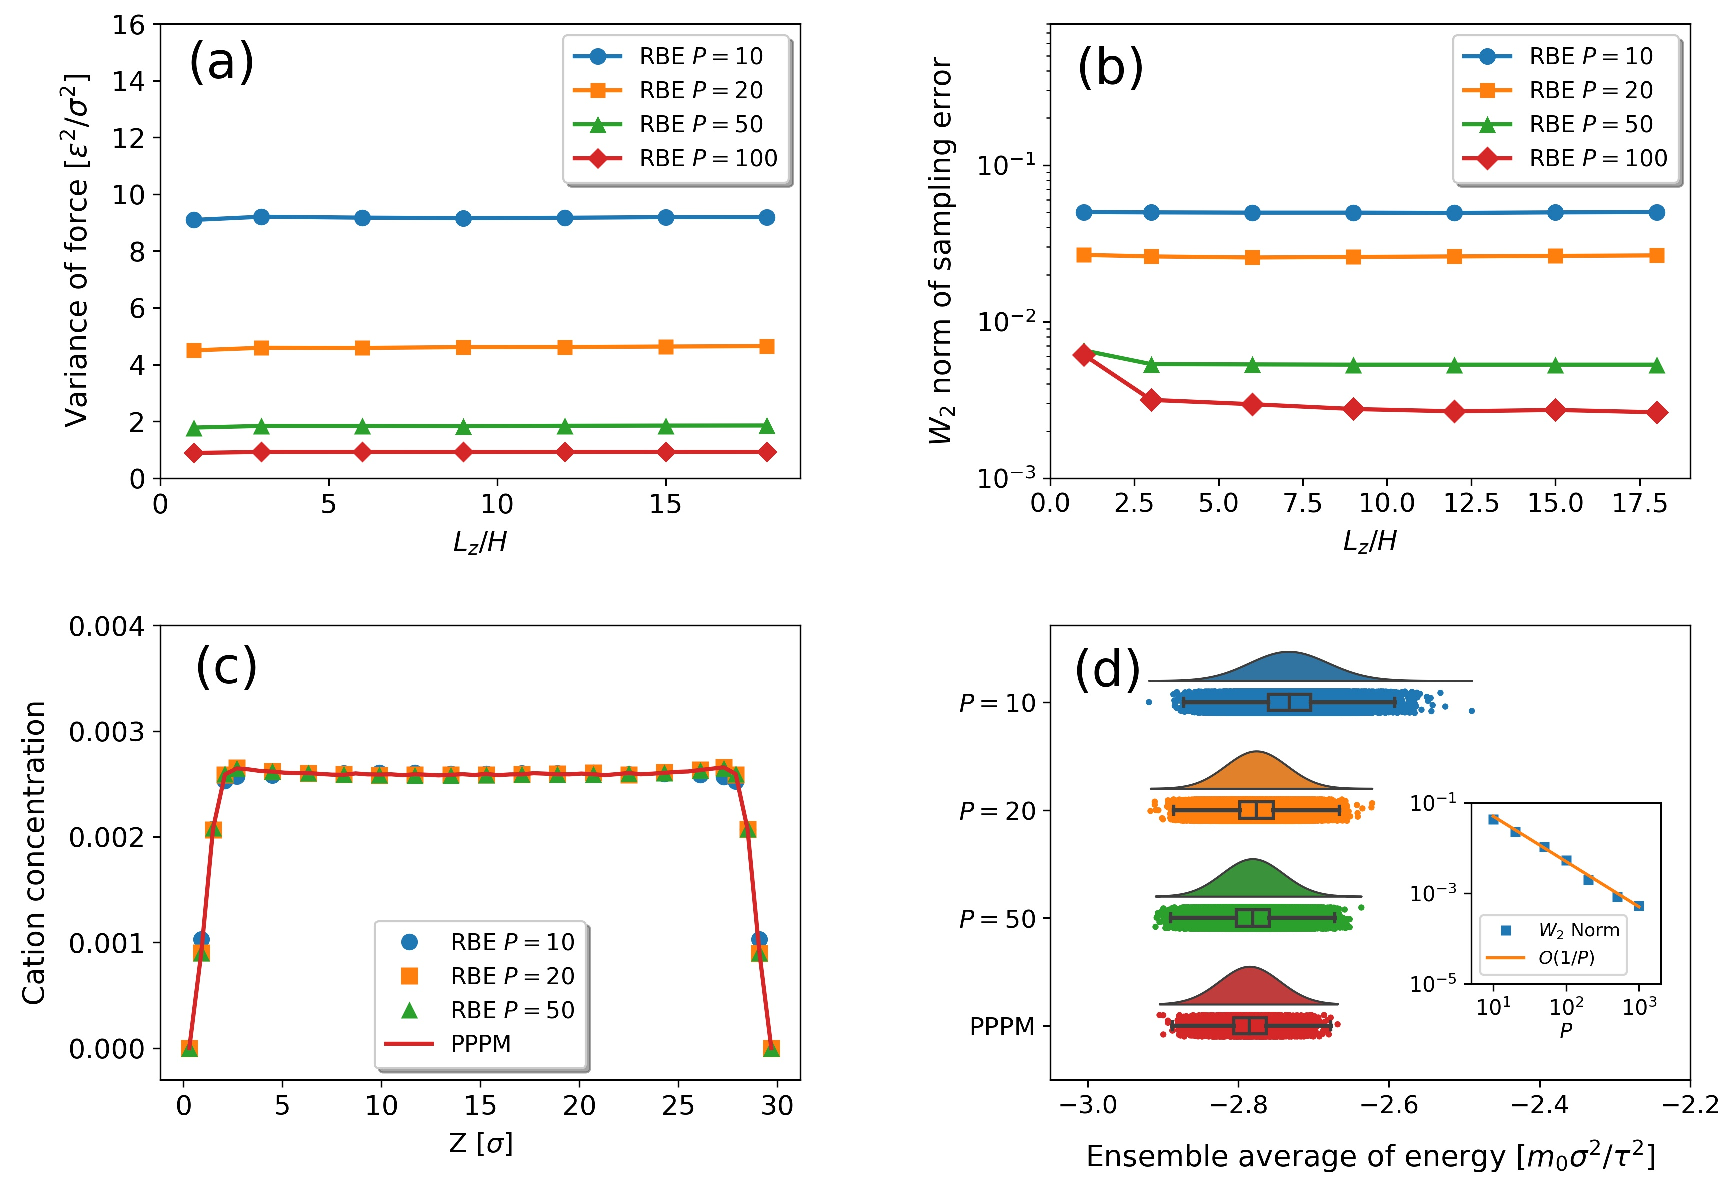
\includegraphics[width=0.90\linewidth]{figs/3_1Elec.pdf}
	\caption{MD results for $3:1$ electrolytes. (a-b):  Variance of force and the error on ensemble average of the potential energy as a function of the relative size of the extended system, $L_z/H$. (c):  Concentration of cations along $z$-dimension. (d):  Raincloud plots of the ensemble average distribution of the potential energy as well as a boxplot and raw data-points. In (a), (c) and (d), results are shown for the RBE2D with different batch size {s} $P$ and the PPPM. In (b), we use the $W_2$ norm defined in Eq.~\eqref{eq::W2} to measure the difference between two distributions. The inset in (d) shows the convergence on the $W_2$ norm with $\mathcal{O}(1/P)$ rate.}
	\label{fig:3_1}
\end{figure}

First, we consider the ensemble average of the variance in forces, denoted as $\langle\|\mathbb{E}|\bm{\Xi}_i|^2\|_{\infty}\rangle$, as shown in Fig.~\ref{fig:3_1}(a). 
Clearly, the force variance is independent   {of} the vacuum layer thickness parameter $L_z$, which validates our theoretical result stated in Theorem~\ref{Thm::1}. 
 {Then we compared the distributions of the potential energy of the obtained samples by the RBE2D and PPPM methods, denoted as~$\mathscr{P}_{\text{RBE}}(\V{x})$ and $\mathscr{P}_{\text{PPPM}}(\V{y})$, respectively.
The Wasserstein-2 norm~\cite{santambrogio2015optimal, kolbe_2024_10912241} is used to measure the difference between two distributions, defined as:}
\begin{equation}\label{eq::W2}
    W_2(\mathscr{P}_{\text{RBE}}, \mathscr{P}_{\text{PPPM}})=\left(\inf _{\gamma \in \Pi(\mathscr{P}_{\text{RBE}}, \mathscr{P}_{\text{PPPM}})} \int|\bm{x} - \bm{y}|^2 d  {\gamma(\bm{x},\bm{y})}\right)^{1 / 2}\;,
\end{equation}
where $\Pi(\mathscr{P}_{\text{RBE}}, \mathscr{P}_{\text{PPPM}})$ represents the set of all joint distributions with marginal distributions $\mathscr{P}_{\text{RBE}}$ and $\mathscr{P}_{\text{PPPM}}$.
The corresponding results are shown Fig.~\ref{fig:3_1}(b), where the~$W_2$ norms are   {plotted} as functions of~$L_z / H$ with   {varying} batch size~$P$.
According to the error estimination in Section~\ref{sec:error_reform}, when $L_z\approx H$, the errors coming from the ELC and remainder error term are still large and can not be ignored;   {this} is consistent with the error decay observed here. 
We also find that, as $L_z\geq 3H$, the error no longer decreases as $L_z/H$ increases (with $P$ fixed); indicating that
both ELC and remainder error terms now indeed become negligible, and the error primarily comes from the random batch approximation. 
%Therefore, when the batch size $P$ is fixed, the error no longer decreases as $L_z/H$ grows beyond a certain extent.


Finally, the concentration of trivalent ions along $z$ and the distribution of energy are investigated.
%with different batch sizes and $L_z/H$ fixed to be $3$, demonstrating the capability of the RBE2D to accurately reproduce the spatial structure and the ensemble averages. 
The corresponding results are depicted in Fig.~\ref{fig:3_1}(c-d). 
We observe a convergence rate of $\mathcal{O}(1/P)$ in the average energy by the RBE2D (with that of the PPPM set as benchmark value). 
This is consistent with our theoretical prediction Theorem~\ref{Thm::1} as the energies of both Coulomb and LJ scale quadratically in displacement near equilibrium.
It is also noticed that, for the RBE2D method, choosing $P=50$ can already yield very accurate results, almost indistinguishable from those obtained via PPPM. 
 {Theorem~\ref{thm::2} also indicates that the error bound in the potential energy of the RBE2D method should converge linearly in $\Delta t$. 
 As numerically validated in Fig.~\ref{fig:energy2d_3_1}, the error indeed decays with $\mathcal{O}(\Delta t)$ scaling. However, this $\mathcal{O}(\Delta t)$ scaling may not hold when $\Delta t$ is larger or in more complicated molecular models. 
 In those scenarios, increasing \(\Delta t\) can lead to particles coming very close to one another (even with the presence of the LJ potential), introducing additional sources of error in other MD components—particularly in managing bond, angle, and dihedral constraints~\cite{frenkel2023understanding}. These artificial effects may result in unphysically large forces or even cause the simulation to fail.}
%Furthermore, we observe a 

\subsection{Dielectrically confined electrolytes}

%To demonstrate the accuracy of the RBE2D method in MD simulations with planar dielectric 
Here we examine four distinct electrolyte systems that are confined by two dielectric interfaces.
These systems include 2:1 and 3:1 electrolytes with varying surface charge densities and dielectric contrasts.
In these systems, all ions are modeled as soft spheres of diameter $r_{\text{d}}$, and are confined by purely repulsive shifted-truncated LJ walls ($\varepsilon_{\text{ion-wall}}=k_{\text{B}}T$; $\sigma_{\text{ion-wall}}=0.5r_{\text{d}}$) at $z=0$ and $z=H$. More detailed information regarding the system settings can be found in Table~\ref{Table::Dielec}.
The MD simulations utilize a time step $0.005\tau$, with temperature controlled by a NH thermostat %using an external temperature of $T=1$ and 
with a damping time of $0.05\tau$,  {where $\tau$ is the reduced LJ unit of time defined in Section \ref{subsec::electrolyte-neutral}}.
All simulations start with an equilibration period of $10^6$ time steps, followed by a production period of $10^8$ time steps.

\begin{figure}[ht!]
\centering
	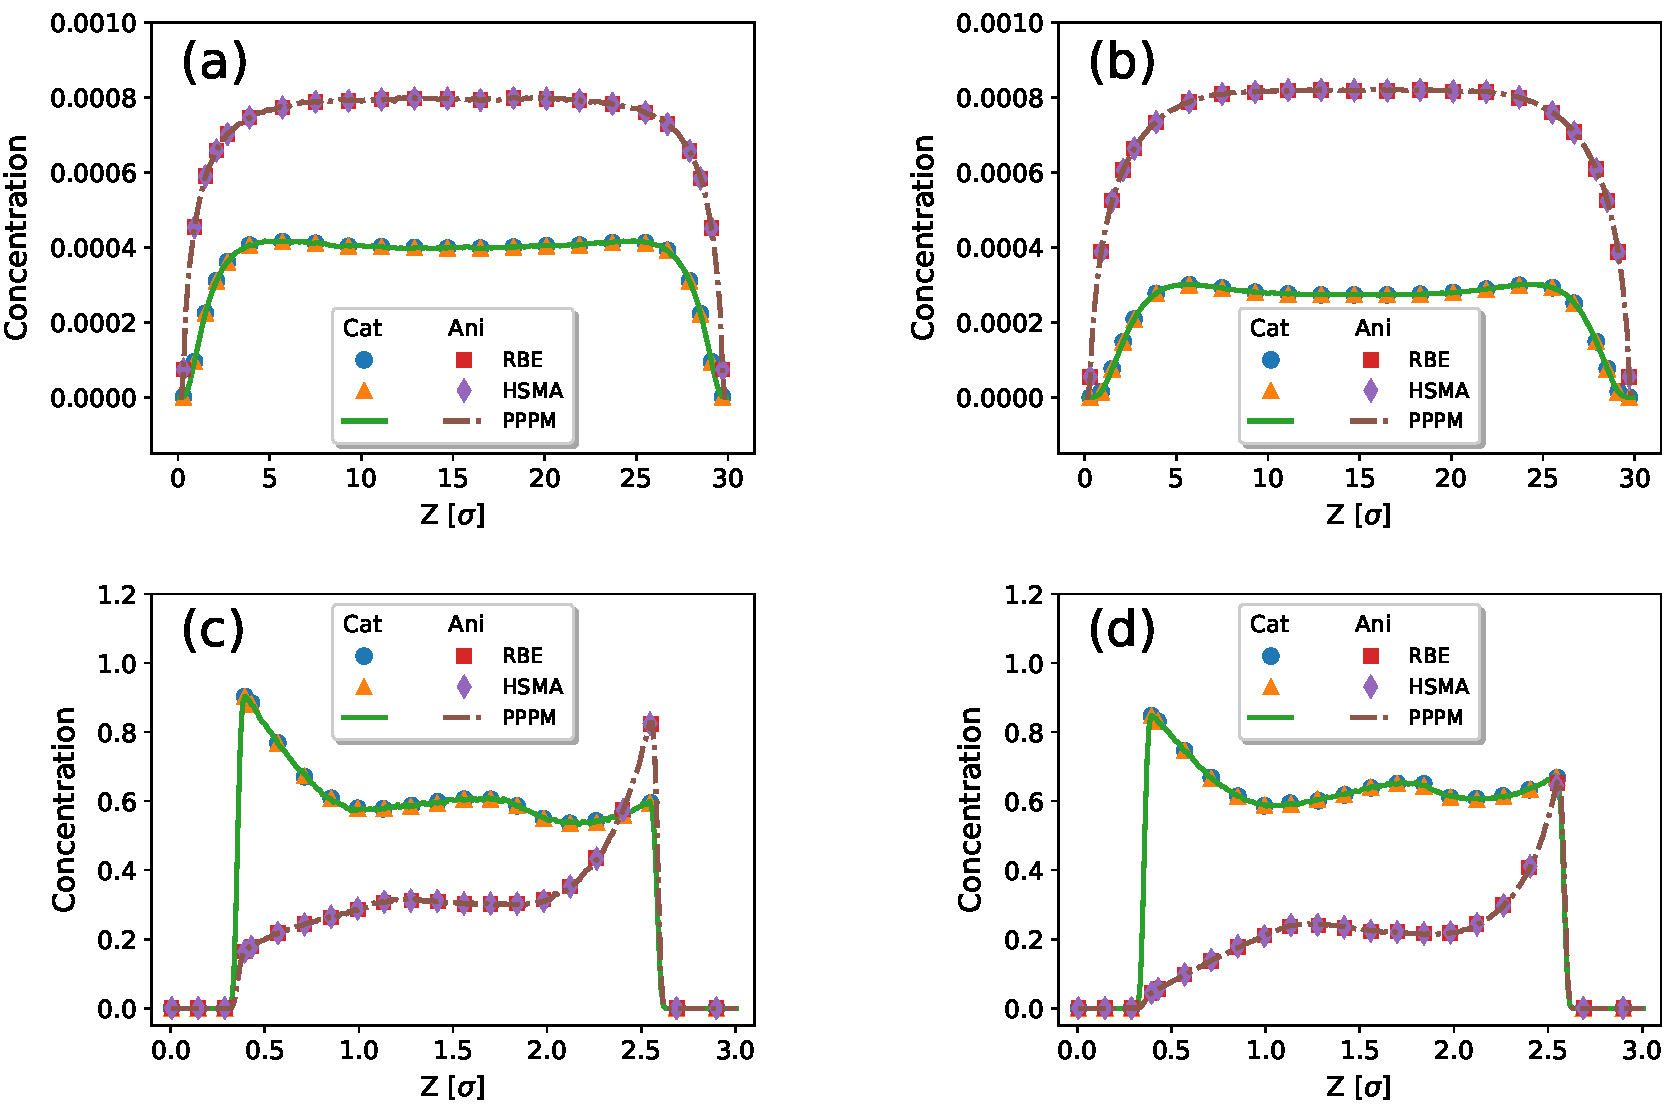
\includegraphics[width=0.95\linewidth]{figs/DistributionDie.pdf}
	\caption{Ionic distributions for [(a) $2:1$ electrolyte and (b) $3:1$ electrolyte] between neutral interfaces with symmetric dielectric contrast, and [(c) $2:1$ electrolyte and (d) $3:1$ electrolyte] confined between walls with asymmetric dielectric contrasts and non-neutral asymmetric surface charge densities. More details about the system settings are provided in Tab.~\ref{Table::Dielec}. 
    Data   {is} shown for the RBE2D method with batch size $P=100$, and the HSMA and the ICM-PPPM methods with relative error threshold $10^{-4}$.} 
	\label{fig:den1}
\end{figure}

We first calculate the cation and anion distributions along  {the} $z$-axis for all considered systems, the results are summarized in Figure~\ref{fig:den1}(a-d). 
In panels (a-b), where the dielectric contrasts are set as $\gamma_{\text{top}}=\gamma_{\text{bot}}=0.939$, the concentrations illustrate the so-called ``ion depletion effect'' near the insulator-like interfaces, consistent with previous findings. 
%In panels (C-D), it is observed that the presence of surface charge modulates this repulsive effect, with the modulation arising from the addition of counterions to maintain charge neutrality. 
Panels (c-d) demonstrate the complicated interplay between the dielectric confinement effect, interfacial charges, and ion valences, and their accumulative effects on the cation distribution. %while these effects mutually reinforce each other for the anion distribution.
For all cases considered, the RBE2D results show excellent agreement with that of the HSMA and ICM-PPPM methods. 
%A comparison with the HSMA and ICM-PPPM methods shows excellent agreement with the RBE2D results. 
The ion distribution shown in panel (c) also agrees with the result from a boundary element solver~\cite{wu2018asymmetric}, and reported in \cite{yuan2021particle}, figure 4(b). 
Additionally, we calculate the potential energy distribution $\mathscr{P}(U)$ for these systems and measure the discrepancy using the $W_2$ norm.
A convergence rate of $\mathcal{O}(1/P)$ is again observed (see Fig.~\ref{fig:energy2d}).

\subsection{CPU time performance}
We now report the CPU time performance of the RBE2D method, compared to the PPPM method. 
The SPC/E bulk water systems are simulated, where
the system dimensions are set as $L_x=L_y=H$,  and the system size changes as one varies $N$ with the density of water being fixed at $1g/cm^3$. For a fair comparison, a cutoff of $10\mathring{A}$ and a relative error threshold of $10^{-4}$ are set for both methods.

%To ensure a fair comparison, we adopt the parameter selection strategy used in the PPPM method, establishing a relative error threshold of $10^{-4}$. For the RBE2D method, we set the Ewald splitting parameter $\alpha$ and the real space cutoff distance $r_c$ to match those of the PPPM method. Additionally, we select batch sizes of $P=100$ and $P=200$ for the RBE2D method, which have been confirmed to provide sufficient accuracy in previous sections.}
% For a fair comparison, a relative error threshold of $10^{-4}$ is set for both methods. 

\begin{figure}[ht!]
\centering	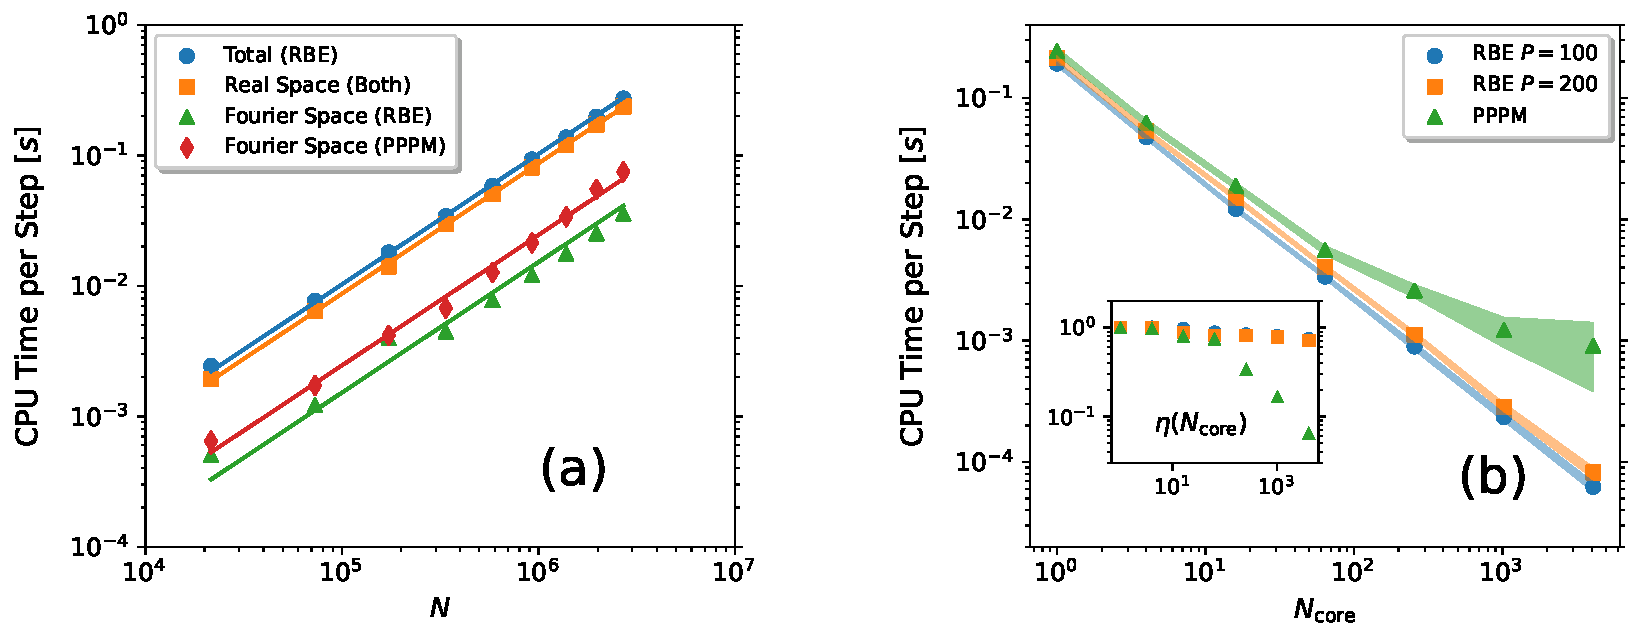
\includegraphics[width=0.9\linewidth]{figs/cpu_time_nonsub.pdf}
	\caption{
     (a) CPU time per step for the RBE2D method  {and PPPM method} with increasing $N$ and (b) total CPU time for comparison between the RBE2D and the PPPM with the number of CPU cores $N_{\emph{core}}$ up to $1024$.  {The results in (a) are obtained} with $64$ cores and $P=100$, where  {the real space cost is identical for both methods by fixing the same Ewald splitting parameter $\alpha$ and real space cutoff $r_c$.}
     The solid lines indicate linear-scaling. 
     In (b), data   {is} shown for the RBE2D with batch size $P=100$ and $P=200$ and the PPPM, where the light-colored parts stand for the range of error bar. The inset in (b) shows the   {strong parallel efficiency} $\eta(N_{\emph{core}})$.}
	\label{fig:Time}
\end{figure}

We first investigate the time cost and complexity by varying particle number $N$. 
In Fig.~\ref{fig:Time}(a), $64$ CPU cores are used, and the  CPU time per MD step for the RBE2D  {and the PPPM method} is documented with particle number $N$ up to $2\times 10^6$, where  {the real space CPU cost is identical for both methods by fixing the same Ewald splitting parameter $\alpha$ and real space cutoff $r_c$}.
 {It should be noted that the main goal of such parameter choice is for solely comparing the improvement of the RBE2D in Fourier space. We expect a fine tuning of $\alpha$ and other parameters to balance the cost of the RBE2D in real and Fourier spaces can further optimize its efficiency in practice.}
The results clearly  {demonstrate} the $\mathcal{O}(N)$ complexity of the RBE2D method  {and its significant advantage over the PPPM method in the Fourier space computation.}
 {A more detailed comparison is further provided in Fig.~\ref{fig:timenondie}, where we compared the performance of each components of the RBE2D and PPPM methods with CPU cores fixed to be both $64$ and $1024$. The results show the improvement of the RBE2D method in the Fourier component computation across the entire range of particle numbers $N$, especially when utilizing a larger number of CPU cores.} %For the PPPM method, the communication cost grows rapidly in $N_{\mathrm{cores}}$, so that the $\mathcal{O}(N\log N)$ complexity is not observed when $N_{\mathrm{cores}}=1024$.} 
%\todo{do we need a reference here}
%For  {the PPPM method}, the CPU time of the real space and the Fourier space computations are balanced to  {achieve optimal efficiency.} 
% {For the RBE2D method, in order to illustrate its advantage in reducing the Fourier space cost compared to the PPPM method, we use the same Ewald parameter $\alpha$ and real space cutoff $r_c$ as PPPM to make sure that the real space cost is identical.
% {Fig.~\ref{fig:timenondie} demonstrates that the RBE2D method significantly reduces CPU time costs compared to the PPPM method, particularly in the Fourier component across the entire range of particle numbers $N$, especially when utilizing a larger number of CPU cores.}


%demonstrating the attractive performance of the algorithm. 
% {It is important to note that the costs associated with the real space and Fourier space computations of the RBE2D method, as shown in Fig.~\ref{fig:Time}(a), are not entirely balanced. This is due to the use of the same parameters $\alpha$ and $r_c$ as those in the PPPM method for a fair comparison. The performance of the RBE2D method can be further enhanced by optimizing the parameters $\alpha$, $r_c$, and $P$.}

Next, we compare the RBE2D and PPPM methods, in terms of both
CPU time performance and  {parallel} scalability. % one of key issues limiting both system scale and time scale of MD simulations. 
%The scalability of the RBE2D method via the strong scaling, characterizing the parallel performance tuning the number of CPU cores by fixing the system size. 
Let  {$N_{\text{core}}$ be the number of cores utilized}, and $T(N_{\text{core}})$ the corresponding CPU time.  {The parallel efficiency for a strong scaling experiment is defined as}
\begin{equation}\label{eq::etau}
\eta(N_{\text{core}})=\frac{N_{\text{min}}}{N_{\text{core}}}\frac{T_{\text{min}}}{T(N_{\text{core}})},
\end{equation}
where $T_{\text{min}}=T(N_{\text{min}})$ and $N_{\text{min}}$ is the minimal number of CPU used. 
Fig.~\ref{fig:Time}(b) and its inset document the CPU time and strong scaling results by the RBE2D and PPPM methods, for a system comprising $139968$ atoms. Clearly,
the two methods perform similarly when $N_{\text{core}}$ is small; and RBE2D outperforms PPPM as $N_{\text{core}}$ increases, the advantage becomes significant for $N_{\text{core}}>64$. Notably,
when $N_{\text{core}}\geq 1024$, RBE2D is approximately 10 times faster than PPPM. 
Furthermore, the strong scaling of the RBE2D remains over $70\%$ when~$\sim 4000$ CPUs are employed, while that of the PPPM drops raplidly to $6\%$. 
 {The main difference between these two methods lies in their communication cost. The RBE2D requires only a single global communication for the reduction of $P$ structure factors. In comparison, the PPPM method, due to its use of FFT, requires six sequential rounds of communication to perform both forward and backward Fourier transforms, leading to poor scalability~\cite{fftscalability,arnold2013comparison}.} This highlights the excellent parallel scalability of the RBE2D method. 
%Due to its mesh-free nature, the RBE2D method is expected to exhibit even greater advantages when applied to systems with strong confinement, where $H\ll\min\{L_x,L_y\}$. In such cases, the PPPM method requires more meshes, leading to a loss in efficiency. 
\newpage

\chapter{QEM for Negatively Confined Coulomb Systems}
\label{chp_quasiewald}
In this chapter, we focus on the negatively confined charged systems, where the dielectric interfaces are characterized by a negative permittivity, leading to a reflection factors that are greater than 1, i.e.,~$\abs{\gamma} > 1$.
Due to the strong polarization effect, the electrostatic interaction in such systems is significantly enhanced compared to the bulk systems and resulting in a failure of the image charge method.
To efficiently simulate such systems, we propose a novel method named the quasi-Ewald method (QEM), which properly accounts for the polarization effect and the long-range interaction in the negatively confined systems.

\section{Quasi-Ewald method}

In this section, we present the quasi-Ewald splitting method, a novel decomposition strategy specifically designed for quasi-2D systems with dielectric interfaces. 
We begin by introducing the quasi-Ewald splitting technique and deriving the Green's function in dielectric confined systems, decomposed into its short-range and long-range components.
We then demonstrate how to efficiently compute electrostatic interactions in positively confined quasi-2D systems by combining this approach with random batch sampling, providing detailed analysis of consistency and variance.
Finally, we extend the quasi-Ewald method to handle systems with negative dielectric constants.

% By integrating this approach with random batch sampling, we develop an efficient summation method that achieves linear complexity.
\subsection{Quasi-Ewald splitting}
Firstly, given a fixed point  $\V{r}^\prime=(x^{\prime}, y^{\prime},z^{\prime})$, we decompose   the Dirac delta function into
%%%%%%%%%%%%%%%%%%%%%%%%%%%%%%%%%%%%%%%%%%%%%%%%%%%%%%%%%%
\begin{equation}\label{eq...text...Quasi-EwaldMethod...QuasiEwaldSplitting}
\begin{aligned}
    \delta(\V{r}-\V{r}^\prime) &= \left[\delta (\V{r}-\V{r}^\prime) - {\left( \frac{\alpha}{\pi} \right)} \exp{\left(-\alpha \Norm{\vrho-\vrho^\prime}^2\right)} \delta(z-z^\prime) \right]\\&~~ + {\left( \frac{\alpha}{\pi} \right)} \exp{\left(-\alpha \Norm{\vrho-\vrho^\prime}^2\right)} \delta(z-z^\prime)\;,
    \end{aligned}
\end{equation}
where $\vr:=(\vrho, z):=(x,y,z)$,   $\vrho:=(x,y)$, and $\vrho^\prime:=(x^\prime,y^\prime)$.
 In this formulation, the first term represents  a charge neutral short range kernel centered at $\vr^\prime$, and the second term corresponds to a smooth long range kernel.  We further define  
\begin{equation}\label{eq...text...Kernels}
    \begin{split}
        \sigma_{s}(\V{r}; \vr^\prime) &:= \delta (\V{r}-\V{r}^\prime) - {\left( \frac{\alpha}{\pi} \right)} \exp{\left(-\alpha \Norm{\vrho-\vrho^\prime}^2\right)} \delta(z-z^\prime)\;,\\
        \sigma_{l}(\V{r};\vr^\prime) &:= {\left( \frac{\alpha}{\pi} \right)} \exp{\left(-\alpha \Norm{\vrho-\vrho^\prime}^2\right)} \delta(z-z^\prime)\;,
    \end{split}
\end{equation}
%
%  Consequently, the total charge density in the system can be expressed as 
%
% \begin{equation}
%     \sigma(\vr) = \sum_{\V{m}} \sum_{i = 1}^{N} q_i \left[\sigma_{s}(\V{r} - \V{r}_i + \V{L_m})  +  \sigma_{s}(\V{r} - \V{r}_i + \V{L_m})\right]\;,
% \end{equation}
and  depiction of the decomposition process is provided in Fig.~\ref{fig:QuasiEwaldSplitting}.  
\begin{figure}
    \centering
    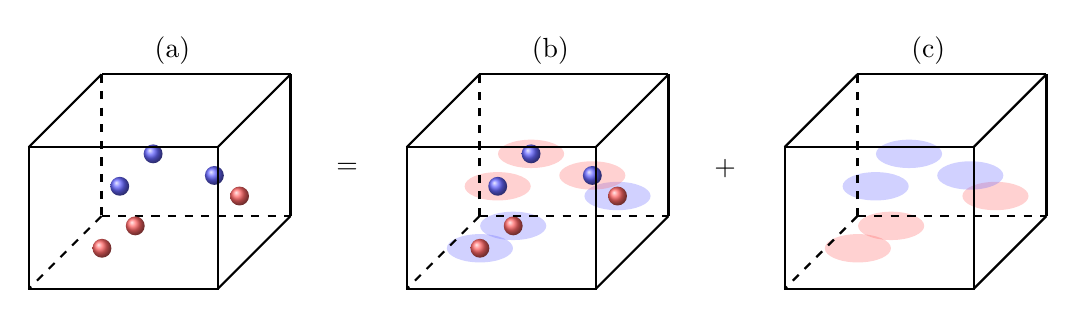
\begin{tikzpicture}[scale = 0.6]

        \def\r{0.2}

        \draw[thick, dashed] (0, 0, 0) -- (4, 0, 0);
        \draw[thick] (4, 0, 0) -- (4, 3, 0);
        \draw[thick] (4, 3, 0) -- (0, 3, 0);
        \draw[thick, dashed] (0, 3, 0) -- (0, 0, 0);


        \foreach \x/\y/\z in {1.1681915835663497/0.4784386449304706/3.0114784670813646, 1.37700874310584/0.4564910752408716/1.723302872827872, 3.730994750135867/1.2345031904085388/2.103105645365449} {
            \shade[ball color=red!60, opacity=1] (\x, \y, \z) circle (\r);
        }

        \foreach \x/\y/\z in {1.827895374334192/2.07357017874381/3.746941345635766, 3.066558538444058/1.5385426337573604/1.7619877149348904, 1.323901301301564/1.5495075401772844/0.6031052215686215} {
            \shade[ball color=blue!60, opacity=1] (\x, \y, \z) circle (\r);
        }

        \draw[thick] (0, 0, 4) -- (4, 0, 4) -- (4, 3, 4) -- (0, 3, 4) -- cycle; % Top face
        \draw[thick, dashed] (0, 0, 0) -- (0, 0, 4); % Front left
        \draw[thick] (4, 0, 0) -- (4, 0, 4); % Front right
        \draw[thick] (4, 3, 0) -- (4, 3, 4); % Back right
        \draw[thick] (0, 3, 0) -- (0, 3, 4); % Back left

        \foreach \x/\y/\z in {1.1681915835663497/0.4784386449304706/3.0114784670813646, 1.37700874310584/0.4564910752408716/1.723302872827872, 3.730994750135867/1.2345031904085388/2.103105645365449} {
            % draw an circle plane laying in the xz plane
            \fill[fill=blue!60, opacity=0.3] (\x + 8, \y, \z) ellipse (0.7 and 0.3);
            \shade[ball color=red!60, opacity=1] (\x + 8, \y, \z) circle (\r);
        }

        \foreach \x/\y/\z in {1.827895374334192/2.07357017874381/3.746941345635766, 3.066558538444058/1.5385426337573604/1.7619877149348904, 1.323901301301564/1.5495075401772844/0.6031052215686215} {
            \fill[fill=red!60, opacity=0.3] (\x + 8, \y, \z) ellipse (0.7 and 0.3);
            \shade[ball color=blue!60, opacity=1] (\x + 8, \y, \z) circle (\r);
        }

        \foreach \x/\y/\z in {1.1681915835663497/0.4784386449304706/3.0114784670813646, 1.37700874310584/0.4564910752408716/1.723302872827872, 3.730994750135867/1.2345031904085388/2.103105645365449} {
            % draw an circle plane laying in the xz plane
            \fill[fill=red!60, opacity=0.3] (\x + 16, \y, \z) ellipse (0.7 and 0.3);
        }

        \foreach \x/\y/\z in {1.827895374334192/2.07357017874381/3.746941345635766, 3.066558538444058/1.5385426337573604/1.7619877149348904, 1.323901301301564/1.5495075401772844/0.6031052215686215} {
            \fill[fill=blue!60, opacity=0.3] (\x + 16, \y, \z) ellipse (0.7 and 0.3);
        }

        \foreach \x/\y/\z in {8/0/0, 16/0/0} {
            \draw[thick, dashed] (\x, \y, \z) -- (4 + \x, \y, \z);
            \draw[thick] (4 + \x, \y, \z) -- (4 + \x, 3 + \y, \z);
            \draw[thick] (4 + \x, 3 + \y, \z) -- (\x, 3 + \y, \z);
            \draw[thick, dashed] (\x, \y, \z) -- (\x, 3 + \y, \z);
            \draw[thick] (\x, \y, 4 + \z) -- (4 + \x, \y, 4 + \z) -- (4 + \x, 3 + \y, 4 + \z) -- (\x, 3 + \y, 4 + \z) -- cycle;
            \draw[thick, dashed] (\x, \y, \z) -- (\x, \y, 4 + \z);
            \draw[thick] (4 + \x, \y, \z) -- (4 + \x, \y, 4 + \z);
            \draw[thick] (4 + \x, 3 + \y, \z) -- (4 + \x, 3 + \y, 4 + \z);
            \draw[thick] (\x, 3 + \y, \z) -- (\x, 3 + \y, 4 + \z);
        }

        \node at (5.2, 1, 0) {$=$};
        \node at (13.2, 1, 0) {$+$};

        \node at (1.5, 3.5, 0) {(a)};
        \node at (9.5, 3.5, 0) {(b)};
        \node at (17.5, 3.5, 0) {(c)};

    \end{tikzpicture}
    \caption{
        An illustration for the quasi-Ewald splitting strategy in a unit cell.
        (a) Charged particles are distributed in the simulation box, cations and anions are represented by red and blue spheres, respectively.
        Sub-figures (b) and (c) shows how Quasi-Ewald splitting works. 
        The discs represent 2D Gaussian charge planes which screen the original point charges.
        We split the original problem into two sub-problems, one with charge neutral particles so that the interactions are short-ranged, another with smooth charge density with a proper geometry so that can be solved rapidly in the reciprocal space.
    }
    \label{fig:QuasiEwaldSplitting}
\end{figure}
Throughout this paper, we will extensively use 2D-Fourier transforms, whose definition is given by
\begin{defination}
    Given function $f(\V{\rho}, z)$, its 2D-Fourier transform is defined by
    \begin{equation}
        \Hat{f}(\V{h}, z):=\int_{\sR^2}f(\V{\rho},z)\exp{(-\mathrm{i} \V{h} \cdot \V{\rho})} d \V{\rho} \;.
    \end{equation}
    The function  $f(\V{\rho}, z)$ can be  recovered from the corresponding inverse 2D-Fourier transform
    \begin{equation} 
        f(\V{\rho}, z)=\frac{1}{4\pi^2}\int_{\sR^2}\Hat{f}(\V{h}, z)\exp{(\mathrm{i} \V{h} \cdot \V{\rho})} d \V{h} \;.
    \end{equation}
\end{defination} 
% \begin{equation}\label{eq...text...FourierTransformKernels}
%     \begin{split}   
%  \hat{\sigma}_{s}(\V{h},z) &=\delta(z)\left[1-\exp\left(-\frac{h^2}{4\alpha}\right)\right]\;,\\
%  \hat{\sigma}_{l}(\V{h},z) &=\delta(z)\exp\left(-\frac{h^2}{4\alpha}\right)\;.
%     \end{split}
% \end{equation}
\begin{prop}
Given fixed point $\V{r}^\prime=(x^{\prime}, y^{\prime},z^{\prime})$, non-zero modes of the 2D-Fourier
transform  of  $ \sigma_{s}(\V{r};\vr^\prime)$ and   $\sigma_{l}(\V{r};\vr^\prime)$  respectively reads
\begin{align*}
 \Hat{\sigma}_{s}(\V{h},z;z^\prime) &= \delta(z-z^\prime) \exp{(-\mathrm{i} \V{h} \cdot \V{\rho}^\prime)}\left(1-\exp\left(-\frac{h^2}{4\alpha}\right)\right)\;,  \\
 \Hat{\sigma}_{l}(\V{h},z;z^\prime) &= \delta(z-z^\prime) \exp{(-\mathrm{i} \V{h} \cdot \V{\rho}^\prime)}\exp\left(-\frac{h^2}{4\alpha}\right)\;,
\end{align*}   
where $\V{h}\neq\vzero$, and the zeroth mode reads
\begin{align*}
 \Hat{\sigma}_{s}(\vzero,z;z^\prime) &= 0\;,  \\
 \Hat{\sigma}_{l}(\vzero,z;z^\prime) &= \delta(z-z^\prime)\;.
\end{align*}   
\end{prop}
\begin{proof}
We observe that for $\V{h}\neq\vzero$, the following integral reads %the  2D-Fourier transform  of $ \sigma_{s}(\V{r}-\vr^\prime)$ reads
\begin{align*}
  % \Hat{\sigma}_{s}(\V{h},z-z^\prime) &=    \int_{\sR^2}\sigma_{s}(\V{r}-\vr^\prime)\exp{(-\mathrm{i} \V{h} \cdot \V{\rho})} d \vrho \\
  % &= \delta(z-z^\prime)\left(
 & \int_{\sR^2}\left[\delta(\vrho-\vrho^\prime)- {\left( \frac{\alpha}{\pi} \right)} \exp{\left(-\alpha \Norm{\vrho-\vrho^\prime}^2\right)}\right] \exp{(-\mathrm{i} \V{h} \cdot \V{\rho})} d \vrho \\
 =&\exp{(-\mathrm{i} \V{h} \cdot \V{\rho}^\prime)}\left[1-  \int_{\sR^2}{\left( \frac{\alpha}{\pi} \right)} \exp{\left(-\alpha \Norm{\vrho-\vrho^\prime}^2\right)}  \exp{(-\mathrm{i} \V{h} \cdot (\V{\rho}-\vrho^\prime))} d \vrho\right]\\
 =&\exp{(-\mathrm{i} \V{h} \cdot \V{\rho}^\prime)}\left(1-\exp\left(-\frac{h^2}{4\alpha}\right)\right)\;,
\end{align*}
hence we obtain that 
\begin{align*}
 \Hat{\sigma}_{s}(\V{h},z;z^\prime) &= \delta(z-z^\prime) \exp{(-\mathrm{i} \V{h} \cdot \V{\rho}^\prime)}\left(1-\exp\left(-\frac{h^2}{4\alpha}\right)\right)\;,  \\
 \Hat{\sigma}_{l}(\V{h},z;z^\prime) &= \delta(z-z^\prime) \exp{(-\mathrm{i} \V{h} \cdot \V{\rho}^\prime)}\exp\left(-\frac{h^2}{4\alpha}\right)\;.
\end{align*}
We observe further that the following integral reads
\begin{align*}
  % \Hat{\sigma}_{s}(\V{h},z-z^\prime) &=    \int_{\sR^2}\sigma_{s}(\V{r}-\vr^\prime)\exp{(-\mathrm{i} \V{h} \cdot \V{\rho})} d \vrho \\
  % &= \delta(z-z^\prime)\left(
 & \int_{\sR^2}\left[\delta(\vrho-\vrho^\prime)- {\left( \frac{\alpha}{\pi} \right)} \exp{\left(-\alpha \Norm{\vrho-\vrho^\prime}^2\right)}\right]  d \vrho \\
 =&\int_{\sR^2}\left[\delta(\vrho-\vrho^\prime)- {\left( \frac{\alpha}{\pi} \right)} \exp{\left(-\alpha \Norm{\vrho-\vrho^\prime}^2\right)}\right]  d \left(\vrho-\vrho^\prime\right) =0\;,
\end{align*}
which finishes the proof.
\end{proof}
% Given $\vr_0:=(\vrho_0,z_0):=(x_0, y_0, z_0)\in\Omega_{\mrm{c}}$,  then the   Poisson's equation reads 
% \begin{equation}\label{eq...text...RepPoisson}
%     \left \{
%     \begin{array}{ll}
%         - \grad_{\V{r}} \cdot\left[ \epsilon(\V{r}) \grad_{\V{r}} G(\V{r},~\V{r}_0) \right] = \delta (\V{r} - \V{r}_0), & \V r \in \mathbb{R}^3 \;, \\
% %%%%%%%%%%%%%%%%%%%%%%%%%%%        
%         G(\V{r},~\V{r}_0) |_{-} = G(\V{r},~\V{r}_0) |_{+}, & \text{on}~\partial\Omega_{\mrm{c}}\;, \\
% %%%%%%%%%%%%%%%%%%%%%%%%%%%        
%           \partial_{z} G(\V{r},~\V{r}_0) |_{-} = \epsilon_{\mrm{u}} \partial_{z} G(\V{r},~\V{r}_0) |_{+}, & \text{on}~\partial \Omega_{\mrm{c}} \cap \partial \Omega_{\mrm{u}}\;,     \\
% %%%%%%%%%%%%%%%%%%%%%%%%%%%            
%   \partial_{z} G(\V{r},~\V{r}_0) |_{-} = \epsilon_{\mrm{d}} \partial_{z} G(\V{r},~\V{r}_0) |_{+}, & \text{on}~\partial \Omega_{\mrm{c}} \cap \partial \Omega_{\mrm{d}}\;,\\
% %%%%%%%%%%%%%%%%%%%%%%%%%%%  
% G(\V{r},~\V{r}_0) \to 0, & \text{as}~{r} \to \infty\;.
% \end{array}\right.
% \end{equation}


Then by employing the Dirichlet to Neumann mapping technique to the Poisson's equation Eq.~\eqref{eq:Poisson_G}, we can derive the Green's function~$G(\V{r}, \V{r_0})$ in the reciprocal space. 

\begin{thm}\label{Proposition...GreensFunction}
    As we define
    \begin{equation}
        \Hat{G}(\V{h}, z; z_0) = \int_{\mathbb{R}^2} G(\V{r}, \V{r_0}) \exp{(-\mathrm{i} \V{h} \cdot \V{\rho})} d \vrho\;,
    \end{equation}     
then for $\V{h}=\vzero$,   
\begin{equation}\label{eq...hat_G_solution...Zeroth}
        \hat{G}(\vzero, z; z_0) = \frac{\abs{z-z_0}}{2}\;,
\end{equation}        
and for $\V{h}\neq \vzero$,     
    \begin{equation}\label{eq...hat_G_solution...Non-zero}
    \begin{aligned}
\hat{G}(\V{h}, z; z_0) &=  \frac{ \exp{(-\mathrm{i} \V{h} \cdot \V{\rho}_0)}}{2 h  \left(1-\gamma_{\mrm{u}}\gamma_{\mrm{d}}\exp(-2 h H)\right)} \sum_{p=1}^4\Gamma_p\exp(- h a_p(z;z_0))\;, %\Big[\exp(-h\abs{z-z_0})\\
% &~~+\gamma_{\mrm{d}}\exp(-h(z+z_0))+\gamma_{\mrm{u}}\exp(-h(2H-z-z_0))\\
% &~~+\gamma_{\mrm{u}}\gamma_{\mrm{d}}\exp(-h(2H-\abs{z-z_0}))\Big]\;.
    \end{aligned}     
    \end{equation}         
where 
\begin{align*}
 \Gamma_{1:4}&:=\left[1,\gamma_{\mrm{d}},\gamma_{\mrm{u}},\gamma_{\mrm{u}}\gamma_{\mrm{d}}\right]\;,\\
 a_{1:4}(z;z_0)&:=\left[\abs{z-z_0}, z+z_0,2H-z-z_0,2H-\abs{z-z_0}\right]\;.
\end{align*}
\end{thm}
\begin{proof}
    By applying Fourier transform on both sides of Eq.~\eqref{eq:Poisson_G}, then for $\V{h}\neq \vzero$, i.e., $k>0$, we obtain that
    \begin{equation*} 
        \begin{split}
            \frac{\partial^2 \Hat{G}_{\mrm{c}}(\V{h}, z; z_0)}{{\partial z}^2} - h^2 \Hat{G}_{\mrm{c}}(\V{h}, z; z_0) = - \frac{ \exp{(-\mathrm{i} \V{h} \cdot \V{\rho}_0)}\delta (z- z_0)}{ }&,~z \in [0, H],\\
            \frac{\partial^2 \hat{G}_{\mrm{u}}(\V{h}, z; z_0)}{{\partial z}^2} - h^2 \hat{G}_{\mrm{u}}(\V{h}, z; z_0) = 0&,~z > H,\\
            \frac{\partial^2 \hat{G}_{\mrm{d}}(\V{h}, z; z_0)}{{\partial z}^2} - h^2 \hat{G}_{\mrm{d}}(\V{h}, z; z_0) = 0&,~z < 0,
        \end{split}
    \end{equation*}
    with the boundary conditions satisfying    
    \begin{equation*}
        \begin{split}
            \Hat{G}_{\mrm{c}}(\V{h}, 0; z_0) &= \Hat{G}_{\mrm{d}}(\V{h}, 0; z_0)\;,\\
            \hat{G}_{\mrm{c}}(\V{h}, H; z_0) &= \hat{G}_{\mrm{u}}(\V{h}, H; z_0)\;,\\
              \partial_z\Hat{G}_{\mrm{c}}(\V{h}, 0; z_0) &= \epsilon_{\mrm{d}} \partial_z\Hat{G}_{\mrm{d}}(\V{h}, 0; z_0)\;,\\
              \partial_z\Hat{G}_{\mrm{c}}(\V{h}, H; z_0) &= \epsilon_{\mrm{u}} \partial_z\Hat{G}_{\mrm{u}}(\V{h}, H; z_0)\;,\\
            \lim_{z \to \infty} \Hat{G}_{\mrm{u}}(\V{h}, z; z_0) &= \lim_{z \to -\infty}\Hat{G}_{\mrm{d}}(\V{h}, z; z_0)  = 0\;,
        \end{split}
    \end{equation*}
based on the infinite boundary condition,  $\Hat{G}_{\mrm{u}}(\V{h}, z; z_0)$ and $\Hat{G}_{\mrm{d}}(\V{h}, z; z_0)$ take the form
\begin{align*}
    \Hat{G}_{\mrm{u}}(\V{h}, z; z_0)&=C_{\mrm{u}}(z_0)\exp(- h z),~z > H\;,\\
     \Hat{G}_{\mrm{d}}(\V{h}, z; z_0)&=C_{\mrm{d}}(z_0)\exp(h z),~~~~z < 0\;,
\end{align*}
therefore, we have 
\begin{align*}
    \partial_z\Hat{G}_{\mrm{u}}(\V{h}, z; z_0)&=-k\Hat{G}_{\mrm{u}}(\V{h}, z; z_0),~z > H\;,\\
     \partial_z\Hat{G}_{\mrm{d}}(\V{h}, z; z_0)&=k\Hat{G}_{\mrm{d}}(\V{h}, z; z_0),~z < 0\;,
\end{align*}
hence the boundary condition can be  simplified into
\begin{align*}
  \partial_z\Hat{G}_{\mrm{c}}(\V{h}, 0; z_0)&=\epsilon_{\mrm{d}} \partial_z\Hat{G}_{\mrm{d}}(\V{h}, 0; z_0)=k\epsilon_{\mrm{d}} \Hat{G}_{\mrm{d}}(\V{h}, 0; z_0)=k\epsilon_{\mrm{d}} \Hat{G}_{\mrm{c}}(\V{h}, 0; z_0)\;,\\
   \partial_z\Hat{G}_{\mrm{c}}(\V{h}, H; z_0)&=\epsilon_{\mrm{u}} \partial_z\Hat{G}_{\mrm{u}}(\V{h}, H; z_0)=-k\epsilon_{\mrm{u}} \Hat{G}_{\mrm{u}}(\V{h}, H; z_0)=-k\epsilon_{\mrm{u}} \Hat{G}_{\mrm{c}}(\V{h}, H; z_0)\;.
\end{align*} 
Finally, for $z\in[0, z_0]$, $\Hat{G}_{\mrm{c}}(\V{h}, z; z_0)$ takes the form
\begin{equation*}
    \Hat{G}_{\mrm{c}}(\V{h}, z; z_0)=\left \{
            \begin{array}{cc}
                \begin{aligned}
                    & A\exp(h z)+B\exp(-h z)\;,
                \end{aligned} & z>z_0, \\
                \begin{aligned}
                 & E\exp(h z)+F\exp(-h z)\;,
                \end{aligned} & z<z_0,
            \end{array}
        \right. \;
\end{equation*}
with $A, B, E, F$ satisfying
\begin{equation}\label{proof...Matrix}
\begin{aligned}
 &A\exp(hz_0)+B\exp(-hz_0)  = E\exp(hz_0)+F\exp(-hz_0)\;,\\
 &A\exp(hz_0)-B\exp(-hz_0)-E\exp(hz_0)+F\exp(-hz_0)=-\frac{ \exp{(-\mathrm{i} \V{h} \cdot \V{\rho}_0)}}{h }\;,\\
 & (E-F)=\epsilon_{\mrm{d}}(E+F)\;,\\
 & \left(A\exp(hH)-B\exp(-hH)\right)=-\epsilon_{\mrm{u}}\left(A\exp(hH)+B\exp(-hH)\right)\;,
\end{aligned}\end{equation}
whose solution reads
\begin{align*}
A&=\frac{ \exp{(-\mathrm{i} \V{h} \cdot \V{\rho}_0)}}{2h }\frac{\exp(-2hH)}{1-\gamma_{\mrm{u}}\gamma_{\mrm{d}}\exp(-2hH)} \left(\gamma_{\mrm{u}}\exp(hz_0)+\gamma_{\mrm{u}}\gamma_{\mrm{d}}\exp(-hz_0)\right)\;,\\
B&=\frac{ \exp{(-\mathrm{i} \V{h} \cdot \V{\rho}_0)} }{2h }\frac{1}{1-\gamma_{\mrm{u}}\gamma_{\mrm{d}}\exp(-2hH)} \left(\exp(hz_0)+\gamma_{\mrm{d}}\exp(-hz_0)\right)\;,\\
E&=A+\frac{\exp{(-\mathrm{i} \V{h} \cdot \V{\rho}_0)} }{2h }\exp(-hz_0)\\
&=\frac{\exp{(-\mathrm{i} \V{h} \cdot \V{\rho}_0)}}{2h }\frac{\gamma_{\mrm{u}}\exp(-2hH)}{1-\gamma_{\mrm{u}}\gamma_{\mrm{d}}\exp(-2hH)} \exp(hz_0)\\&~~+\frac{\exp{(-\mathrm{i} \V{h} \cdot \V{\rho}_0)}}{2h }\frac{1}{1-\gamma_{\mrm{u}}\gamma_{\mrm{d}}\exp(-2hH)}\exp(-hz_0)\;,\\
F&=\frac{\exp{(-\mathrm{i} \V{h} \cdot \V{\rho}_0)}}{2h }\frac{\gamma_{\mrm{u}}\gamma_{\mrm{d}}\exp(-2hH)}{1-\gamma_{\mrm{u}}\gamma_{\mrm{d}}\exp(-2hH)} \exp(hz_0)\\&~~+\frac{\exp{(-\mathrm{i} \V{h} \cdot \V{\rho}_0)}}{2h }\frac{\gamma_{\mrm{d}}}{1-\gamma_{\mrm{u}}\gamma_{\mrm{d}}\exp(-2hH)} \exp(-hz_0)\;,
\end{align*}
 and similar procedures can be applied to the case $\V{h}=\vzero$, we omit this for brevity.
\end{proof}

\begin{rmk}\label{Remark...Nonzero+larger}
    If $\gamma_u \gamma_d < 1$, the determinant of the Eq.~\eqref{proof...Matrix} is non-zero on the positive real axis.
    However, for negatively confined systems with $\gamma_u \gamma_d > 1$, a first order pole exists at $h= \ln(\gamma_u \gamma_d)/2H$ and the Green's function diverges.
    Moreover, it is noteworthy that all the components in $a_{1:4}(z;z_0)$ take positive values. 
\end{rmk}


Based on the decomposition relation Eq.~\eqref{eq...text...Quasi-EwaldMethod...QuasiEwaldSplitting} and definition in Eq.~\eqref{eq...text...Kernels}, we observe that 
\begin{equation}%\label{eq...text...Rewrite-in-kernels}
   \delta(\V{r}-\V{r}_0)=\sigma_s  (\V{r};\V{r}_0)+\sigma_\ell  (\V{r};\V{r}_0)\;,
\end{equation}
and we  shall decompose the Green's function  $ G(\V{r}, \V{r_0})$ correspondingly into
\begin{equation}
    G(\V{r}, \V{r_0})= G_s(\V{r}, \V{r_0})+  G_\ell(\V{r}, \V{r_0})\;,
\end{equation}
where $ G_s(\V{r}, \V{r_0})$ and $  G_\ell(\V{r}, \V{r_0})$ are the solutions to the Poisson's equation Eq.~\eqref{eq:Poisson_G} except that $\delta(\V{r}-\V{r}_0)$ is replaced respectively by $\sigma_s  (\V{r};\V{r}_0)$ and $\sigma_\ell  (\V{r};\V{r}_0)$.
\begin{corollary}
For any $\V{h}\neq \vzero$, given     $\hat{G}(\V{h}, z; z_0)$, we obtain that  
    \begin{align*}
        \hat{G}_s(\V{h}, z; z_0)&=\hat{G}(\V{h}, z; z_0)\left[1-\exp\left(-\frac{h^2}{4\alpha}\right)\right]\;,\\
        \hat{G}_\ell(\V{h}, z; z_0)&=\hat{G}(\V{h}, z; z_0)\exp\left(-\frac{h^2}{4\alpha}\right)\;,
    \end{align*} 
    and for  $\V{h}=\vzero$, given     $\hat{G}(\vzero, z; z_0)$, we obtain that  
        \begin{align*}
        \hat{G}_s(\vzero, z; z_0)&=0\;,\\
        \hat{G}_\ell(\vzero, z; z_0)&=\hat{G}(\vzero, z; z_0)\;.
    \end{align*} 
\end{corollary}
Its proof is straightforward in that we only need to solve out the Systems of Eq.~\eqref{proof...Matrix} by replacing  the coefficient $-\frac{\exp{(-\mathrm{i} \V{h} \cdot \V{\rho}_0)}}{h }$ with  
\begin{equation*}
    -\frac{\exp{(-\mathrm{i} \V{h} \cdot \V{\rho}_0)}}{h }\left[1-\exp\left(-\frac{h^2}{4\alpha}\right)\right]\;,
\end{equation*}
and 
\begin{equation*}
    -\frac{\exp{(-\mathrm{i} \V{h} \cdot \V{\rho}_0)}}{h }\exp\left(-\frac{h^2}{4\alpha}\right)\;,
\end{equation*} 
respectively.
Consequently, the Green's function $ G_s(\V{r}, \V{r_0})$ and $  G_\ell(\V{r}, \V{r_0})$ can be recovered following the inverse Fourier transform of $  \hat{G}_s(\V{h}, z; z_0)$ and $  \hat{G}_\ell(\V{h}, z; z_0)$,
\begin{equation*}
\begin{aligned}
 G_s(\V{r}, \V{r_0})&=   \frac{1}{4\pi^2}\int_{\sR^2} \hat{G}_s(\V{h}, z; z_0)\exp{(\mathrm{i} \V{h} \cdot \V{\rho})} d \V{h}\\
 &= \frac{1}{4\pi^2}\int_{\sR^2} \hat{G}(\V{h}, z; z_0)\left[1-\exp\left(-\frac{h^2}{4\alpha}\right)\right]\exp{(\mathrm{i} \V{h} \cdot \V{\rho})} d \V{h}\;,\\
  G_\ell(\V{r}, \V{r_0})&=   \frac{1}{4\pi^2}\int_{\sR^2} \hat{G}_\ell(\V{h}, z; z_0)\exp{(\mathrm{i} \V{h} \cdot \V{\rho})} d \V{h}\\
 &= \frac{1}{4\pi^2}\int_{\sR^2} \hat{G}(\V{h}, z; z_0)\exp\left(-\frac{h^2}{4\alpha}\right)\exp{(\mathrm{i} \V{h} \cdot \V{\rho})} d \V{h}\;.
\end{aligned}    
\end{equation*}
Hence the total interaction energy reads
\begin{align*}
   U & =   U_s+U_\ell\;,
\end{align*}
whereas
\begin{align}
U_s&:=    \frac{1}{2} {\sum_{\V{m}}}^\prime \sum_{i, j = 1}^{N} q_i q_j G_s(\V{r}_i+\vL_m, \V{r}_j)\;, \label{eq::U_s}\\
U_\ell&:=   \frac{1}{2} {\sum_{\V{m}}}\sum_{i, j = 1}^{N} q_i q_j  G_\ell(\V{r}_i+\vL_m, \V{r}_j)\;. \label{eq::U_l}
\end{align}
Given $\vr_j:=(\vrho_j, z_j)$, then for the short range kernel $G_s(\cdot, \V{r}_j)$, whose expression reads 
\begin{align*}
 &G_s(\V{r}, \V{r}_j)\\
 =&   \frac{1}{4\pi^2}\int_{\sR^2} \hat{G}(\V{h}, z; z_j)\left[1-\exp\left(-\frac{h^2}{4\alpha}\right)\right]\exp{(\mathrm{i} \V{h} \cdot \V{\rho})} d \V{h}\\
 =& \frac{1}{4\pi^2}\int_{\sR^2} \frac{ \exp{(\mathrm{i} \V{h} \cdot (\V{\rho}-\V{\rho}_j))}}{2h \left(1-\gamma_{\mrm{u}}\gamma_{\mrm{d}}\exp(-2hH)\right)} \left[1-\exp\left(-\frac{h^2}{4\alpha}\right)\right]\left[\sum_{p=1}^4\Gamma_p\exp(-ha_p(z;z_j))\right]d \V{h}\;,
% =&\frac{1}{8\pi^2 }\int_{\sR^2} \frac{ \exp{(\mathrm{i} \V{h} \cdot \V{\rho}_{ij})}}{k\left(1-\gamma_{\mrm{u}}\gamma_{\mrm{d}}\exp(-2hH)\right)} \left[1-\exp\left(-\frac{h^2}{4\alpha}\right)\right]\sum_{p=1}^4\Gamma_p\exp(-ha_p(z_i;z_j))d \V{h}\;,
\end{align*}
moreover, if further given $\V{r}_i:=(\vrho_i, z_i)$, we obtain that 
\begin{align*}
   &G_s(\V{r}_i, \V{r}_j)\\
   =& \frac{1}{8\pi^2 }\int_{\sR^2} \frac{ \exp{(\mathrm{i} \V{h} \cdot \V{\rho}_{ij})}}{k\left(1-\gamma_{\mrm{u}}\gamma_{\mrm{d}}\exp(-2hH)\right)} \left[1-\exp\left(-\frac{h^2}{4\alpha}\right)\right]\left[\sum_{p=1}^4\Gamma_p\exp(-ha_p(z_i;z_j))\right]d \V{h}\;,
\end{align*}
where $\V{\rho}_{ij}:=\vrho_i-\vrho_j$. 
In actually calculations, due to the short range nature of~$G_s(\cdot, \V{r}_j)$, the infinite sum in Eq.~\eqref{eq::U_s} is truncated to a finite sum in real space with a cutoff $r_c$, given by
\begin{equation}\label{eq::U_s_truncated}
    U_s \approx U_{s, *} = \sum_{\abs{\bm{\rho}_{ij, m}} \leq r_c} q_i q_j G_s(\V{r}_i+\vL_m, \V{r}_j)\;,
\end{equation}
where $\bm{\rho}_{ij, m}:=\vrho_i-\vrho_j+ (L_x m_x, L_y m_y)$, and the summation indicates that among all possible pairs of particles, only the terms with $\abs{\bm{\rho}_{ij, m}} \leq r_c$ are considered.


 As for the long  range kernel $ G_\ell(\cdot, \V{r}_j)$, based on the Poisson summation formula, we obtain that 
% \begin{align*}
%  & G_\ell(\V{r}_i, \V{r}_j)\\
%  =&   \frac{1}{4\pi^2}\int_{\sR^2} \hat{G}(\V{h}, z_i; z_j)\exp\left(-\frac{h^2}{4\alpha}\right)\exp{(\mathrm{i} \V{h} \cdot \V{\rho}_i)} d \V{h}\\
%  =& \frac{1}{4\pi^2}\int_{\sR^2} \frac{ \exp{(\mathrm{i} \V{h} \cdot (\V{\rho}_i-\V{\rho}_j))}}{2h \left(1-\gamma_{\mrm{u}}\gamma_{\mrm{d}}\exp(-2hH)\right)} \exp\left(-\frac{h^2}{4\alpha}\right)\sum_{p=1}^4\Gamma_p\exp(-ha_p(z_i;z_j))d \V{h}\\
%  =&\frac{1}{8\pi^2 }\int_{\sR^2} \frac{ \exp{(\mathrm{i} \V{h} \cdot \V{\rho}_{ij})}}{k\left(1-\gamma_{\mrm{u}}\gamma_{\mrm{d}}\exp(-2hH)\right)} \exp\left(-\frac{h^2}{4\alpha}\right)\sum_{p=1}^4\Gamma_p\exp(-ha_p(z_i;z_j))d \V{h}\;,
% \end{align*}
\begin{equation}\label{eq...text...PoissonSummation}
 \sum_{\vm}  G_\ell(\V{r}+\vL_m, \V{r}_j)  =\frac{1}{ L_xL_y}   \sum_{\V{h}\in\fK^2} \Hat{G}_\ell(\V{h},z;z_j)\exp(\textrm{i}\V{h}\cdot \vrho) \;,
\end{equation}
where \[\fK^2 := \left\{\V{h} \in \frac{  2\pi}{L_x}\sZ\times \frac{  2\pi}{L_y}\sZ \right\}\;.\]
Furthermore, the RHS of Eq. \eqref{eq...text...PoissonSummation} reads
\begin{align*}
&\frac{1}{ L_xL_y}   \sum_{\V{h}\in\fK^2} \Hat{G}_\ell(\V{h},z;z_j)\exp(\textrm{i}\V{h}\cdot \vrho)\\
%=&\frac{1}{ L_xL_y}  \left( \sum_{\V{h}\in\fK^2}  \hat{G}(\V{h}, z; z_j)\exp\left(-\frac{h^2}{4\alpha}\right)\exp{(\mathrm{i} \V{h} \cdot \V{\rho})} \right)\\
=& \frac{1}{ L_xL_y}   \left[\Hat{G}_\ell(\vzero, z; z_j)+\sum_{\V{h}\in\fK^2,\V{h}\neq\vzero}  \hat{G}_\ell(\V{h}, z; z_j)\exp{(\mathrm{i} \V{h} \cdot \V{\rho})}\right]\\
=&\frac{1}{ L_xL_y}   \left[\hat{G}(\vzero, z; z_j)+\sum_{\V{h}\in\fK^2,\V{h}\neq\vzero}  \hat{G}(\V{h}, z; z_j)\exp\left(-\frac{h^2}{4\alpha}\right)\exp{(\mathrm{i} \V{h} \cdot \V{\rho})}\right]\;,
\end{align*}
therefore, given $\vr_i$, the above expression can be simplified into
\begin{align*}
 &\frac{1}{ L_xL_y}   \sum_{\V{h}\in\fK^2,\V{h}\neq\vzero} \Hat{G}_\ell(\V{h},z;z_j)\exp(\textrm{i}\V{h}\cdot \vrho)\\
 =& \frac{1}{ L_xL_y}   \sum_{\V{h}\in\fK^2,\V{h}\neq\vzero} \frac{ \exp{(\mathrm{i} \V{h} \cdot \V{\rho}_{ij})}}{2h \left(1-\gamma_{\mrm{u}}\gamma_{\mrm{d}}\exp(-2hH)\right)}\left[\sum_{p=1}^4\Gamma_p\exp(-ha_p(z_i;z_j))\right] \exp\left(-\frac{h^2}{4\alpha}\right)\;,
\end{align*}
to sum up, the energy $U_\ell$ reads
\begin{align*}
    U_\ell&=\frac{1}{2}\sum_{\vm}\sum_{i,j=1}^N q_iq_j G_\ell(\V{r}_i+\vL_m, \V{r}_j)\\
    &=\frac{1}{4  L_xL_y}\sum_{i,j=1}^N  q_iq_j \Bigg({\Abs{z_i-z_j}} +\\&~~~~+  \sum_{\V{h}\in\fK^2,\V{h}\neq\vzero} \frac{ \exp{(\mathrm{i} \V{h} \cdot \V{\rho}_{ij})}}{k\left(1-\gamma_{\mrm{u}}\gamma_{\mrm{d}}\exp(-2hH)\right)}\left[\sum_{p=1}^4\Gamma_p\exp(-ha_p(z_i;z_j))\right] \exp\left(-\frac{h^2}{4\alpha}\right)\Bigg)\;.
\end{align*}


\subsection{The algorithm}

We first consider the case where the dielectric constants of the upper and lower regions are positive, i.e., $\gamma_{\mrm{u}} \gamma_{\mrm{d}} < 1$. 
In this part, we develop fast algorithms for numerically evaluating both the short-range and long-range parts of the interaction energy.

First we consider the short-range part $U_s$.
We observe that the energy $U_s$ is constituted by the terms
\begin{align*}
  &G_s(\V{r}_i, \V{r}_j)\\
   =& \frac{1}{8\pi^2 }\int_{\sR^2} \frac{ \exp{(\mathrm{i} \V{h} \cdot \V{\rho}_{ij})}}{k\left(1-\gamma_{\mrm{u}}\gamma_{\mrm{d}}\exp(-2hH)\right)} \left[1-\exp\left(-\frac{h^2}{4\alpha}\right)\right]\left[\sum_{p=1}^4\Gamma_p\exp(-ha_p(z_i;z_j))\right]d \V{h}\;,  
\end{align*}
in which $\vr_i$ and $\vr_j$ are given, and we further notice  that all the components in $G_s(\V{r}_i, \V{r}_j)$ take the form
\begin{equation}\label{eq::int_Gs}
    \begin{split}
        & \int_{\sR^2} \frac{ \exp{(\mathrm{i} \V{h} \cdot \V{\rho}_{ij})}}{k\left(1-\gamma_{\mrm{u}}\gamma_{\mrm{d}}\exp(-2hH)\right)} \left[1-\exp\left(-\frac{h^2}{4\alpha}\right)\right]\exp(-ha_p(z_i;z_j))d \V{h}\\
        =2\pi&\int_0^{+\infty} \frac{ \exp(-ha_p(z_i;z_j))}{1-\gamma_{\mrm{u}}\gamma_{\mrm{d}}\exp(-2hH)} \left[1-\exp\left(-\frac{h^2}{4\alpha}\right)\right] J_0(\rho_{ij}k)d k\;,
    \end{split}
\end{equation}
where $\rho_{ij}:=\Norm{\vrho_{ij}}=\Norm{\vrho_i-\vrho_j}$, and $ J_0(\cdot)$ is the zeroth-order Bessel function,  which  can   be expressed as a complex contour integral over a full period.
\begin{defination}
    The zeroth-order Bessel function of the first kind, denoted by $ J_0(r)$, is formally defined via the integral representation
\begin{equation}
       J_0(r):=\frac{1}{2\pi} \int_0^{2\pi} \exp(\mathrm{i} r\sin \theta) d \theta\;.  
    \end{equation}
\end{defination}
We proceed to evaluate the following integral
\begin{equation}\label{eq...text...InfiniteIntegral}
\int_0^{+\infty} \frac{ \exp(-ah)}{1-\gamma_{\mrm{u}}\gamma_{\mrm{d}}\exp(-2hH)} \left[1-\exp\left(-\frac{h^2}{4\alpha}\right)\right] J_0(\rho h)d k\;,    
\end{equation}
where $a>0$ and $\rho>0$ are fixed constants. Firstly, we observe that Eq. \eqref{eq...text...InfiniteIntegral} can be written into
\begin{align*}
   & \int_0^{+\infty} \frac{ \exp(-ah)}{1-\gamma_{\mrm{u}}\gamma_{\mrm{d}}\exp(-2hH)} \left[1-\exp\left(-\frac{h^2}{4\alpha}\right)\right] J_0(\rho h)d k\\
   =&\underbrace{\int_0^{+\infty} \frac{1}{1-\gamma_{\mrm{u}}\gamma_{\mrm{d}}\exp(-2hH)}  \exp(-ah)  J_0(\rho h)d k}_{\text{Term}~\mathrm{I}}\\
   &-\underbrace{\int_0^{+\infty} \frac{1}{1-\gamma_{\mrm{u}}\gamma_{\mrm{d}}\exp(-2hH)}\exp\left(-\frac{h^2}{4\alpha}\right)  \exp(-ah)  J_0(\rho h)d k}_{\text{Term}~\mathrm{II}}\;.
\end{align*}
Secondly, we observe further that Term $\mathrm{I}$ can be decomposed into
\begin{align*}
&\int_0^{+\infty} \frac{1}{1-\gamma_{\mrm{u}}\gamma_{\mrm{d}}\exp(-2hH)}  \exp(-ah)  J_0(\rho h)d k\\
=&\underbrace{\int_0^{+\infty}   \exp(-ah)  J_0(\rho h)d k}_{\text{Term}~\mathrm{I(a)}}\\
&+\underbrace{\int_0^{+\infty} \frac{\gamma_{\mrm{u}}\gamma_{\mrm{d}}}{1-\gamma_{\mrm{u}}\gamma_{\mrm{d}}\exp(-2hH)}  \exp(-2hH)\exp(-ah)  J_0(\rho h)d k}_{\text{Term}~\mathrm{I(b)}}\;,
\end{align*}
on the basis of the identity
\begin{equation*}
    \int_0^{+\infty}\exp(-ax) J_0(x)d x=\frac{1}{\sqrt{a^2+1}}\;,
\end{equation*}
then Term $\mathrm{I(a)}$ can be simplified into 
\begin{equation}\label{eq...text...TermI(A)}
    \int_0^{+\infty}   \exp(-ah)  J_0(\rho h)d k=\frac{1}{\sqrt{a^2+\rho^2}}\;.
\end{equation}
It is observed that Term $\mathrm{I(b)}$ and Term $\mathrm{II}$  comprise infinite integrals involving rapidly decaying functions coupled with oscillatory components. To efficiently evaluate such integrals over an infinite domain, we employ the method proposed in \cite{trefethen2022exactness}, which facilitates numerical computation by truncating the integration region to a finite domain. 
% \begin{thm}[Theorem 5.1 in \cite{trefethen2022exactness}]\label{Thm...Truncation}
%  Let $f(x)$ be analytic and bounded for $x \in(-\infty, \infty)$, and suppose $F(x):=\exp \left(-x^2\right) f(x)$ extends to a bounded analytic function in the infinite strip $-a<\operatorname{Im} x<$ a for some $a>0$. Let $L>0$ be fixed, and for each $n \geq 1$, as we denote  \[I_n(F):=\sum_{j=1}^n w_jF(x_j)\;,\] as the estimate of the integral \[I(F):=\int_{-\infty}^{+\infty} F(x)d x \;,\]  obtained by applying Gauss-Legendre, Clenshaw-Curtis, or equispaced trapezoidal quadrature on the truncated interval $\left[-L n^{1 / 3}, L n^{1 / 3}\right]$. Then for some $C>0$,  the following holds 
%  \begin{equation}
%  \left|I-I_n\right|=\fO\left(\exp \left(-C n^{2 / 3}\right)\right), \quad n \rightarrow \infty\;.  
%  \end{equation}
% \end{thm}
For any given 
$M>0$, as the infinite integral can be decomposed into
\begin{equation*}
 \int_0^{+\infty} F(k)d  k=  \int_0^{M} F(k)d  k+\int_M^{+\infty} F(k)d  k\;,
\end{equation*} 
then the first part of the integral can be efficiently evaluated  using  Gauss-Legendre quadrature, while the second integral can be neglected for sufficiently large $M$. To ensure   validity of such truncation, it is necessary to provide some  estimates on the associated truncation error as a function of $M$.
% For the Term $\mathrm{I(b)}$, its truncation error reads
%
% \begin{equation}\label{eq...text...TruncationError(Term1(b))}
% \begin{aligned}
%     &\Abs{\int_M^{+\infty} \frac{\gamma_{\mrm{u}}\gamma_{\mrm{d}}}{1-\gamma_{\mrm{u}}\gamma_{\mrm{d}}\exp(-2hH)}  \exp(-2hH)\exp(-ah)  J_0(\rho h)d k}\\
%     \leq &  \frac{\Abs{\gamma_{\mrm{u}}\gamma_{\mrm{d}}}}{1-\max\{0,\gamma_{\mrm{u}}\gamma_{\mrm{d}}\}}\int_M^{+\infty}  \exp(-2hH)) \Abs{ J_0(\rho h)}d k
% \end{aligned}    
% \end{equation}
\begin{prop}
We denote the     truncation errors of Term $\mathrm{I(b)}$ and Term $\mathrm{II}$ respectively by
\begin{align*}
  \delta \mathrm{I}_b(M)&:=\int_M^{+\infty} \frac{\gamma_{\mrm{u}}\gamma_{\mrm{d}}}{1-\gamma_{\mrm{u}}\gamma_{\mrm{d}}\exp(-2hH)}  \exp(-2hH)\exp(-ah)  J_0(\rho h)d k \;,\\  
  \delta \mathrm{II}(M)&:=\int_M^{+\infty}  \frac{1}{1-\gamma_{\mrm{u}}\gamma_{\mrm{d}}\exp(-2hH)}\exp\left(-\frac{h^2}{4\alpha}\right)  \exp(-ah)  J_0(\rho h)d k \;,
\end{align*}
whose estimates read
\begin{align}
    \Abs{\delta \mathrm{I}_b(M)} &\leq  \frac{\Abs{\gamma_{\mrm{u}}\gamma_{\mrm{d}}}}{1-\max\{0,\gamma_{\mrm{u}}\gamma_{\mrm{d}}\}}\frac{1}{\sqrt{\rho H}}\mrm{erfc}(\sqrt{2HM})\;,\\
    \Abs{\delta \mathrm{II}(M)} &\leq \frac{\sqrt{2\alpha} }{1-\max\{0,\gamma_{\mrm{u}}\gamma_{\mrm{d}}\}} \mrm{erfc}\left(\frac{M}{2\sqrt{\alpha}}\right)\;.
\end{align}
\end{prop}
\begin{proof}
We obtain immediately that for $r>0$ large enough,     
\begin{equation*}
   \Abs{ J_0(r)}\leq \sqrt{\frac{2}{\pi}} \frac{1}{\sqrt{r}}\;, 
\end{equation*}
thus we have 
\begin{align*}
   & \int_M^{+\infty}  \exp(-2hH)\exp(-ah)  J_0(\rho h)d k \\
\leq & \int_M^{+\infty}  \exp(-2hH)\sqrt{\frac{2}{\pi}} \frac{1}{\sqrt{\rho h}} d k=\frac{1}{\sqrt{\rho H}}\mrm{erfc}(\sqrt{2HM})\;,
\end{align*}
and 
\begin{align*}
  &\int_M^{+\infty}  \exp\left(-\frac{h^2}{4\alpha}\right)  \exp(-ah)  J_0(\rho h)d k \\
  \leq &\int_M^{+\infty} \exp\left(-\frac{h^2}{4\alpha}\right)\sqrt{\frac{2}{\pi}} \frac{1}{\sqrt{\rho h}} d k\\ 
  \leq &\int_M^{+\infty} \exp\left(-\frac{h^2}{4\alpha}\right)\sqrt{\frac{2}{\pi}} d k=\sqrt{2\alpha} \mrm{erfc}\left(\frac{M}{2\sqrt{\alpha}}\right)\;,
\end{align*}
and we finish our proof.
\end{proof}

As validations, we compared the errors in calculating the oscillatory integral $\int_0^{\infty} J_0(x \rho) \exp{(-x)} \mrm{d}x$ and $\int_{-\infty}^{\infty} J_0(x \rho) \exp{(-x^2)} \mrm{d}x$ using the Gauss-Laguerre/Gauss-Hermite quadrature or the Gauss-Legendre quadrature.
First for a fixed~$\rho = 50$, as shown by Fig.~\ref{fig:Gauss_int} (a) and (b), the truncated Gauss-Legendre formula on interval~$[0, 36]$ or~$[-6, 6]$ converge much rapidly as the number of points~$n$ increase comparing to the Gauss-Laguerre or Gauss-Hermite formula.
Then for varying~$\rho \in [0, 10]$, we set~$E = 4$, $8$ and $12$, and compute number of points needed for the truncated Gauss-Legendre formula to reach the given accuracy~$E$.
As shown in Fig.~\ref{fig:Gauss_int_n} (a) and (b), in both cases the integrals converge rapidly and only take a few tens of points the reach the accuracy.
In this way, both~$I_1$ and~$I_2$ are transformed to be integrals on finite region and can be evaluated easily using the Gauss–Legendre formula.

\begin{figure}[htbp]
    \centering
    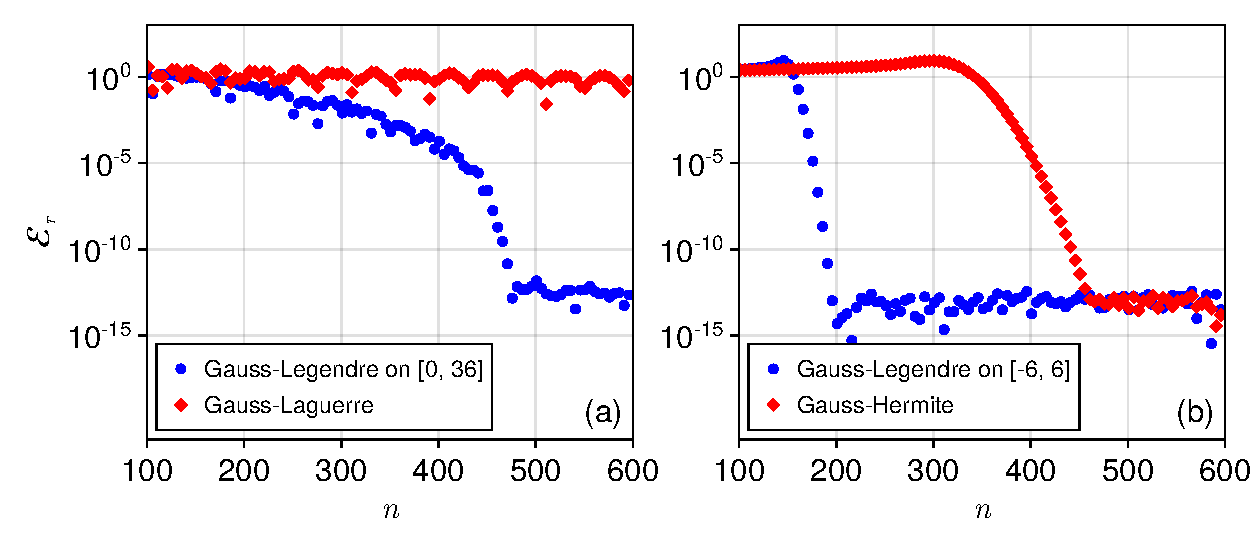
\includegraphics[width = \linewidth]{figs/integral_n.pdf}
    \caption{
        The relative error of numerical evaluation of integrals~$\int_0^{\infty} J_0(50 x) \exp{(-x)} \mrm{d}x$ and~$\int_{-\infty}^{\infty} J_0(50 x) \exp{(-x^2)} \mrm{d}x$ via (a) Gauss–Laguerre quadrature and (b) Gauss–Hermite quadrature on infinite interval or Gauss-Legendre quadrature on truncated interval,~$n$ is the order of the quadrature.
    }
    \label{fig:Gauss_int}
\end{figure}

\begin{figure}[htbp]
    \centering
    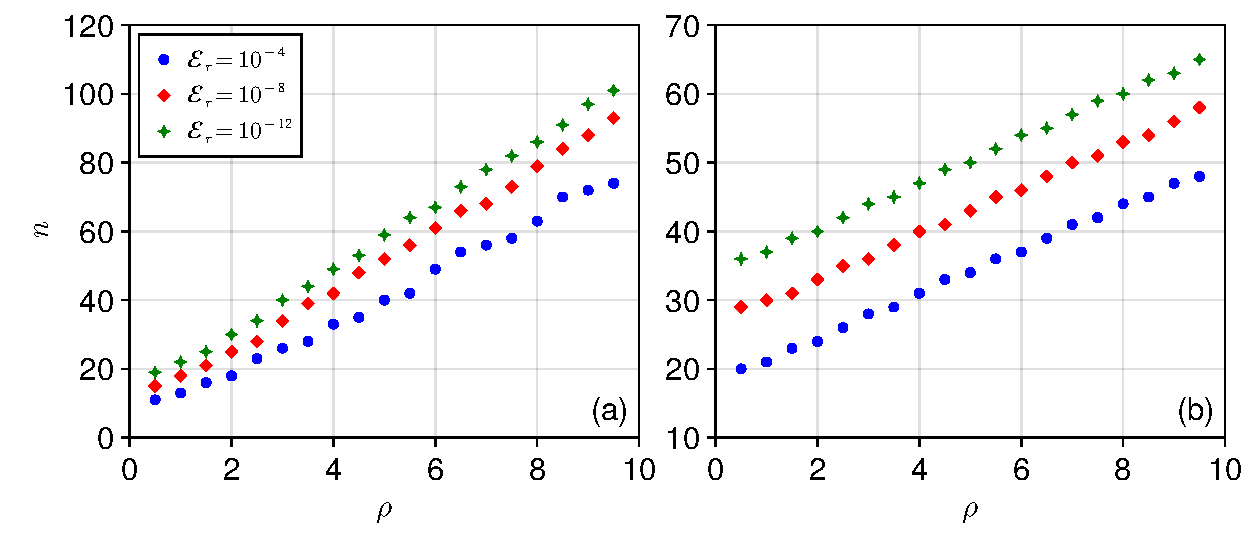
\includegraphics[width = \linewidth]{figs/integral_r.pdf}
    \caption{
    Order of quadrature~$n$, needed to numerically evaluate (a)~$\int_0^{\infty} J_0(\rho x) \exp{(-x)} \mrm{d}x$ and (b)~$\int_{-\infty}^{\infty} J_0(\rho x) \exp{(-x^2)} \mrm{d}x$ to reach the given relative accuracy~$\mathcal{E}_r$ using the Gauss-Legendre quadrature on truncated interval~$[0, k_{c1}]$ and~$[-k_{c2}, k_{c2}]$, respectively, where~$\rho \in [0, 10]$ determine the strength of the oscillation and~$k_{c1/2}$ are determined by~$E$.
    }
    \label{fig:Gauss_int_n}
\end{figure}

Then we consider the long-range part~$U_\ell$.
As the long range interaction  energy $U_\ell$ reads
\begin{align*} 
U_\ell&=\frac{1}{4  L_xL_y}\sum_{i,j=1}^N q_iq_j\Bigg({\Abs{z_i-z_j}} +\\&~~~~+  \sum_{\V{h}\in\fK^2,\V{h}\neq\vzero} \frac{ \exp{(\mathrm{i} \V{h} \cdot \V{\rho}_{ij})}}{k\left(1-\gamma_{\mrm{u}}\gamma_{\mrm{d}}\exp(-2hH)\right)}\left[\sum_{p=1}^4\Gamma_p\exp(-ha_p(z_i;z_j))\right] \exp\left(-\frac{h^2}{4\alpha}\right)\Bigg)\;,
\end{align*}
and we endeavor to  reduce the $\fO(N^2)$ complexity to linear scaling by incorporating the idea of random batch sampling in combination with the technique that has been discussed in Chapter~\ref{chp_soewald2d}.

%Firstly, we shall deal with the summation over $i$ and $j$, i.e., $\sum_{i,j=1}^N$. 
We observe that the four components in the following summation read
\begin{align*}
     &\sum_{p=1}^4\Gamma_p\exp(-ha_p(z_i;z_j))\\  
     =&\exp(- h \Abs{z_i-z_j})+\gamma_{\mrm{d}}\exp(-h(z_i+z_j))\\
     &+\gamma_{\mrm{u}}\exp(-h(2H-z_i-z_j)) +\gamma_{\mrm{u}}\gamma_{\mrm{d}}\exp(-h(2H-\Abs{z_i-z_j}))\;.
\end{align*}
%%%%%%%%%%%%%%%%%%%%%%%%%%%%%%%%%%%%%%%%%%%%%%%%%%%%%%%%%%
To facilitate the computation, we define auxiliary functions $\beta_{1:4}(h)$ as 
\begin{align*}
    \beta_1(\V{h})&:= \frac{1}{4  L_xL_yk\left(1-\gamma_{\mrm{u}}\gamma_{\mrm{d}}\exp(-2hH)\right)} \;,\\
    \beta_2(\V{h})&:= \frac{\gamma_{\mrm{d}}}{4  L_xL_yk\left(1-\gamma_{\mrm{u}}\gamma_{\mrm{d}}\exp(-2hH)\right)} \;,\\
    \beta_3(\V{h})&:= \frac{\gamma_{\mrm{u}}\exp(-2hH)}{4  L_xL_yk\left(1-\gamma_{\mrm{u}}\gamma_{\mrm{d}}\exp(-2hH)\right)}\;,\\
    \beta_4(\V{h})&:= \frac{\gamma_{\mrm{u}}\gamma_{\mrm{d}}\exp(-2hH)}{4  L_xL_yk\left(1-\gamma_{\mrm{u}}\gamma_{\mrm{d}}\exp(-2hH)\right)}\;,
\end{align*}
and another set of auxiliary functions   $S_{0:4}(k)$ as
%which allows us to express the summation over $i$ and $j$ in  $U_\ell$ as
\begin{align*} 
    S_0&:=\frac{1}{4  L_xL_y}\sum_{i,j=1}^Nq_iq_j {\Abs{z_i-z_j}}\;,\\
    S_1(\V{h})&:=\sum_{i,j=1}^Nq_iq_j  \exp{(\mathrm{i} \V{h} \cdot \V{\rho}_{ij})}\exp(-h\Abs{z_i-z_j})\;,\\
    S_2(\V{h})&:=\sum_{i,j=1}^Nq_iq_j  \exp{(\mathrm{i} \V{h} \cdot \V{\rho}_{ij})}\exp(-h(z_i+z_j))\;,\\
    S_3(\V{h})&:=\sum_{i,j=1}^Nq_iq_j  \exp{(\mathrm{i} \V{h} \cdot \V{\rho}_{ij})}\exp(h(z_i+z_j))\;,\\
    S_4(\V{h})&:=\sum_{i,j=1}^Nq_iq_j \exp{(\mathrm{i} \V{h} \cdot \V{\rho}_{ij})}\exp(h\Abs{z_i-z_j})\;.
\end{align*}
Consequently, the long-range interaction energy   $U_\ell$ reads
\begin{equation}\label{eq...text...Energy}
    U_\ell = S_0+ \sum_{\V{h}\in\fK^2,\V{h}\neq\vzero} \exp\left(-\frac{h^2}{4\alpha}\right)\sum_{p=1}^4S_p(\V{h}) \beta_p(\V{h})\;.
\end{equation}
and for simplicity, we denote hereafter in this paper that 
\begin{equation}\label{eq...text...phi}
    \phi(\V{h}):=\sum_{p=1}^4S_p(\V{h}) \beta_p(\V{h})\;,
\end{equation}
and on the basis of Eq. \eqref{eq...text...phi}, the   energy   $U_\ell$ can be simplified into 
\begin{equation} \label{eq...text...EnergywithPhi}
U_\ell =    S_0+ \sum_{\V{h}\in\fK^2,\V{h}\neq\vzero} \phi(\V{h})\exp\left(-\frac{h^2}{4\alpha}\right) \;,
\end{equation}
and the idea of random batch sampling is employed to efficiently evaluate the summation over   $\V{h}$, i.e., $\sum_{\V{h}\in\fK^2,\V{h}\neq\vzero}$. 
%However, prior to this step, we shall  introduce some alignment techniques to further enhance computational efficiency.
% \subsubsection{Part One: Pairwise summation}
It is easy to observe that  the  auxiliary functions  $S_2(\V{h})$ and $S_3(\V{h})$ are multiplicatively separable  in the sense that  they can be written into
\begin{align*}
S_2(\V{h})&=\sum_{i,j=1}^Nq_iq_j  \exp{(\mathrm{i} \V{h} \cdot \V{\rho}_{ij})}\exp(-h(z_i+z_j))\\
&=\left(\sum_{i=1}^Nq_i\exp{(\mathrm{i} \V{h} \cdot \V{\rho}_{i})}\exp(-hz_i)\right)\left(\sum_{j=1}^Nq_j\exp{(-\mathrm{i} \V{h} \cdot \V{\rho}_{j})}\exp(-hz_j)\right)\;,\\
S_3(\V{h})&=\sum_{i,j=1}^Nq_iq_j  \exp{(\mathrm{i} \V{h} \cdot \V{\rho}_{ij})}\exp(h(z_i+z_j))\\
&=\left(\sum_{i=1}^Nq_i  \exp{(\mathrm{i} \V{h} \cdot \V{\rho}_{i})}\exp(hz_i)\right)\left(\sum_{j=1}^Nq_j  \exp{(-\mathrm{i} \V{h} \cdot \V{\rho}_{j})}\exp(hz_j)\right)\;,
\end{align*}
such factorization significantly reduces computational complexity, as the direct evaluation of the double summation requires 
$\fO(N^2)$ operations, whereas the factorized form allows computation in only 
$\fO(N)$ steps.

However, the functions $S_0$,  $S_1(\V{h})$ and $S_4(\V{h})$  are non-multiplicatively separable due to the presence of the absolute difference term $\abs{z_i - z_j}$ which prevents direct factorization. Consequently, the strategy employed for 
$S_2(\V{h})$ and $S_3(\V{h})$ is no longer applicable. To achieve linear computational complexity in evaluating these terms,  some specialized alignment techniques must be introduced.

Firstly, we sort all $N$ particles according to their positions along the 
$z$-axis, ensuring the ordering
\begin{equation*}
   0 < z_1 < z_2 <  \cdots <  z_{N - 1}<z_N < H\;.
\end{equation*}
Since for all  $i$, $z_i \in (0, H)$ is uniformly bounded, hence  the strategies such as the bucket sorting~\cite{corwin2004sorting} can be applied, and the computational cost can be of order~$\mathcal{O}(N \log{N})$ or even  of order~$\mathcal{O}(N)$. Once all $N$ particles are sorted according to their positions along the 
$z$-axis, we observe that $S_0$ can be written into
\begin{align*}
    S_0 
    & = \sum_{i = 1}^N q_i \left( \sum_{j = 1}^{i }{q_j (z_i - z_j)} \right) \\
    & = 2 \sum_{i = 1}^N q_i \left( z_i \sum_{j = 1}^{i }q_j - \sum_{j = 1}^{i }z_j q_j  \right) \;.
\end{align*}
To efficiently compute this summation, we introduce two auxiliary sequences  $\left\{T_1(i)\right\}_{i=1}^N$ and $\left\{T_2(i)\right\}_{i=1}^N$, both of which  can be iteratively updated as follows:
\begin{align*}
    &T_1(1)=q_1,~~T_1(i+1)=T_1(i)+q_{i+1}\;,\\
    &T_2(1)=z_1q_1,~~T_2(i+1)=T_2(i)+z_{i+1}q_{i+1}\;.
\end{align*}
Using these auxiliary sequences, 
$S_0$ can be efficiently calculated as
\[
S_0= 2 \sum_{i = 1}^N q_i \left( z_iT_1(i)-T_2(i)\right)\;,
\]
which requires only 
$4N$ operations, significantly reducing computational complexity in comparison with the naive summation.

A similar strategy~\cite{jiang2021approximating, gan2024fast} can also be applied to the evaluation of $S_1(\V{h})$ and $S_4(\V{h})$. For $S_1(\V{h})$, we obtain that 
\begin{align*}
S_1(\V{h})&=\sum_{i,j=1}^Nq_iq_j  \exp{(\mathrm{i} \V{h} \cdot \V{\rho}_{ij})}\exp(-h\Abs{z_i-z_j})\\
&=-\sum_{i=1}^Nq_i^2+\sum_{i=1}^N \sum_{j=1}^iq_iq_j  \exp{(\mathrm{i} \V{h} \cdot \V{\rho}_{ij})}\exp(-h(z_i-z_j))\\
&~~+\sum_{i=1}^N \sum_{j=i}^Nq_iq_j  \exp{(\mathrm{i} \V{h} \cdot \V{\rho}_{ij})}\exp(-h(z_j-z_i))\\
&= -\sum_{i=1}^Nq_i^2+\sum_{i=1}^N q_i\exp{(\mathrm{i} \V{h} \cdot \V{\rho}_{i})}\exp(-hz_i)\sum_{j=1}^iq_j\exp{(-\mathrm{i} \V{h} \cdot \V{\rho}_{j})}\exp(hz_j)\\
&~~+\sum_{i=1}^N q_i\exp{(\mathrm{i} \V{h} \cdot \V{\rho}_{i})}\exp(hz_i)\sum_{j=i}^Nq_j\exp{(-\mathrm{i} \V{h} \cdot \V{\rho}_{j})}\exp(-hz_j)\;,
\end{align*}
 we introduce another two auxiliary sequences  $\left\{T_3(i)\right\}_{i=1}^N$ and $\left\{T_4(i)\right\}_{i=1}^N$, and it is noteworthy that $\left\{T_3(i)\right\}_{i=1}^N$ is  constructed through forward iteration, whereas  $\left\{T_4(i)\right\}_{i=1}^N$   is generated through backward iteration:

\begin{align*}
    &T_3(1)=q_1\exp{(-\mathrm{i} \V{h} \cdot \V{\rho}_{1})}\exp(hz_1)\;,\\
    &T_3(i+1)=T_3(i)+q_{i+1}\exp{(-\mathrm{i} \V{h} \cdot \V{\rho}_{i+1})}\exp(hz_{i+1})\;,\\
    &T_4(N)=q_N\exp{(-\mathrm{i} \V{h} \cdot \V{\rho}_{N})}\exp(-hz_N)\;,\\
    &T_4(i-1)=T_4(i)+q_{i-1}\exp{(-\mathrm{i} \V{h} \cdot \V{\rho}_{i-1})}\exp(-hz_{i-1})\;,
\end{align*}
and
$S_1(\V{h})$ can be efficiently calculated as
\[
S_1(\V{h})= -\sum_{i=1}^Nq_i^2+ \sum_{i=1}^N q_i\exp{(\mathrm{i} \V{h} \cdot \V{\rho}_{i})}\left[\exp(-hz_i)T_3(i)+\exp(hz_i)T_4(i)\right]\;.
\]
As for $S_4(\V{h})$, we shall follow the same routine:
\begin{align*}
S_4(\V{h})&=\sum_{i,j=1}^Nq_iq_j  \exp{(\mathrm{i} \V{h} \cdot \V{\rho}_{ij})}\exp(-h\Abs{z_i-z_j})\\
&=-\sum_{i=1}^Nq_i^2+\sum_{i=1}^N \sum_{j=1}^iq_iq_j  \exp{(\mathrm{i} \V{h} \cdot \V{\rho}_{ij})}\exp(h(z_i-z_j))\\
&~~+\sum_{i=1}^N \sum_{j=i}^Nq_iq_j  \exp{(\mathrm{i} \V{h} \cdot \V{\rho}_{ij})}\exp(h(z_j-z_i))\\
&= -\sum_{i=1}^Nq_i^2+\sum_{i=1}^N q_i\exp{(\mathrm{i} \V{h} \cdot \V{\rho}_{i})}\exp(hz_i)\sum_{j=1}^iq_j\exp{(-\mathrm{i} \V{h} \cdot \V{\rho}_{j})}\exp(-hz_j)\\
&~~+\sum_{i=1}^N q_i\exp{(\mathrm{i} \V{h} \cdot \V{\rho}_{i})}\exp(-hz_i)\sum_{j=i}^Nq_j\exp{(-\mathrm{i} \V{h} \cdot \V{\rho}_{j})}\exp(hz_j)\;,
\end{align*}
and we introduce another two auxiliary sequences  $\left\{T_5(i)\right\}_{i=1}^N$ and $\left\{T_6(i)\right\}_{i=1}^N$, and it is noteworthy that $\left\{T_5(i)\right\}_{i=1}^N$ is  constructed through forward iteration, whereas  $\left\{T_6(i)\right\}_{i=1}^N$   is generated through backward iteration:

\begin{align*}
    &T_5(1)=q_1\exp{(-\mathrm{i} \V{h} \cdot \V{\rho}_{1})}\exp(-hz_1)\;,\\
    &T_5(i+1)=T_5(i)+q_{i+1}\exp{(-\mathrm{i} \V{h} \cdot \V{\rho}_{i+1})}\exp(-hz_{i+1})\;,\\
    &T_6(N)=q_N\exp{(-\mathrm{i} \V{h} \cdot \V{\rho}_{N})}\exp(hz_N)\;,\\
    &T_6(i-1)=T_6(i)+q_{i-1}\exp{(-\mathrm{i} \V{h} \cdot \V{\rho}_{i-1})}\exp(hz_{i-1})\;,
\end{align*}
and $S_4(\V{h})$ can be written as
\[
S_4(\V{h})= -\sum_{i=1}^Nq_i^2+ \sum_{i=1}^N q_i\exp{(\mathrm{i} \V{h} \cdot \V{\rho}_{i})}\left[\exp(hz_i)T_5(i)+\exp(-hz_i)T_6(i)\right]\;.
\]
To sum up, given fixed frequency $\V{h}^\ast$, it only takes  linear complexity to evaluate $S_0$ and $\phi(\V{h}^\ast)$, and we proceed to deal with the   summation over $\V{h}$. 
% \subsubsection{Part Two: Random Batch Importance Sampling}

% Then we introduce a stochastic algorithm designed to accelerate the Quasi-Ewald method in particle simulations, reducing the complexity to $\mathcal{O}(N)$. 
% Unlike existing methods relying on either FFT or FMM-based techniques to reduce the complexity, our idea involves adopting mini-batch stochastic approximation over Fourier modes, with importance sampling for variance reduction. 
% More precisely, let us consider the Fourier sum over $\bm k \in \mathcal{K}^2$ for a given kernel $f(\bm{k})$,
% one can alternatively understand the Fourier sum as an expectation
% \begin{equation}
% 	\mu:=\sum_{\bm{k}\in\mathcal{K}^2}\frac{f(\bm{k})}{g(\bm{k})}g(\bm{k})=\mathbb{E}_{\bm k\sim g(\bm{k})}\left[\frac{f(\bm{k})}{g(\bm{k})}\right],
% \end{equation}
% where $g(\bm{k})$ is a probability measure defined on the lattice $\bm k \in \mathcal{K}^2$ and the expectation~$\mathbb{E}_{\bm k\sim g(\bm{k})}$ is taken with respect to the probability measure.
% Instead of calculating the summation directly or using FFT, a mini-batch of Fourier modes (with batch size $P$) sampled from $g(\bm{k})$ are employed to estimate the expectation, resulting in an efficient stochastic algorithm.

% It is worth noting that the random mini-batch strategy originated from stochastic gradient descent in machine learning and was first introduced in the study of interacting particle systems by Jin et al.~\cite{jin2020random}, called the random batch method. 
Observe that the long-range interaction energy $U_\ell$ can be represented as
\[
U_\ell =   S_0+ \sum_{\V{h}\in\fK^2,\V{h}\neq\vzero}\phi(\V{h}) \exp\left(-\frac{h^2}{4\alpha}\right) \;,
\]
we define 
\begin{equation}\label{eq::U_l0_Ulk}
    U_\ell^{\vzero} := S_0,\quad\text{and}\quad U_\ell^{\V{h}\neq \vzero} :=\sum_{\V{h}\in\fK^2,\V{h}\neq\vzero}\phi(\V{h}) \exp\left(-\frac{h^2}{4\alpha}\right) \;,
\end{equation}
then $U_\ell$ can be written into the sum of these two components
\[
U_\ell= U_\ell^{\vzero}+U_\ell^{\V{h}\neq \vzero}\;,
\]
Since 
$ U_\ell^{\vzero}$
can be computed with linear complexity, we focus on the efficient evaluation of 
$U_\ell^{\V{h}\neq \vzero}$, for which the idea of random batch is employed.
Based on the above expression, we find a Gaussian decay factor in $U_\ell^{\V{h}\neq \vzero}$ explicitly, which can be normalized for the  purpose of importance sampling, so that again we apply the idea of random batch sampling taking
\begin{equation}\label{eq::hk}
	g(\bm{k}) := \frac{1}{S} \exp\left(-\frac{h^2}{4\alpha}\right)\;, %\quad H := \sum_{\bm{k}\neq\bm{0}}e^{-h^2/(4\alpha^2)},
\end{equation}
where \[S:= \sum_{\V{h}\in\fK^2,\V{h}\neq\vzero}\exp\left(-\frac{h^2}{4\alpha}\right)\;,\] serves as a normalization factor.
% By application of the Poisson summation formula, $H$ can be computed as follows
%
% \begin{align*}
%   H+1&=  \sum_{\V{h}\in\fK^2}\exp\left(-\frac{h^2}{4\alpha}\right)\;,\\
%   \sum_{\V{h}\in\fK^2}\exp\left(-\frac{h^2}{4\alpha}\right)&= \frac{\alpha L_xL_y}{\pi}\sum_{m_x,m_y\in\mathbb{Z}}\exp\left({-\alpha\left(m_x^2L_x^2+m_y^2L_y^2\right)}\right)\;,
% \end{align*}
%
% hence
%
% \begin{equation}\label{eq::Happ}
% 	H=-1+\frac{\alpha L_xL_y}{\pi}\sum_{m_x,m_y\in\mathbb{Z}}\exp\left({-\alpha\left(m_x^2L_x^2+m_y^2L_y^2\right)}\right)\;,
% \end{equation}
%
Using the Metropolis algorithm~\cite{metropolis1953equation}, a random mini-batch of frequencies $\{\bm{k}_{\eta}\}_{\eta=1}^P$ is sampled, where~$P$ is the batch size, and $U_\ell$ can be approximated as 
\begin{equation}\label{eq::RBapp}
 U_\ell^{\V{h}\neq \vzero} \approx U_{l,\ast}^{\V{h}\neq \vzero}  :=   \frac{S}{P}\sum_{\eta=1}^P \phi(\V{h}_{\eta})=  \frac{S}{P}\sum_{\eta=1}^P \sum_{q=1}^4S_q(\V{h}_{\eta})h_q(\V{h}_{\eta})\;,
\end{equation} 
and the corresponding estimator of the force in Fourier space is given by
\begin{equation}
	 \bm{F}_{l,i}\approx\bm{F}_{l,i}^*=-  \grad_{\V{r}_i} U_\ell^{\vzero}- \grad_{\V{r}_i} U_{l,\ast}^{\V{h}\neq \vzero}\;,
 \end{equation}
Finally, combining all these strategies, we state our Quasi-Ewald method for calculating the electrostatic energy and forces in molecular dynamics simulations, see Algorithm~\ref{alg:rbqe}.
\begin{algorithm}[ht] 
\caption{The Quasi-Ewald method}
\begin{algorithmic}[1]
    \State \textbf{Input}:  Initialize the size of the simulation box $(L_x,L_y, H)$, as well as the positions, velocities, and charges of all particles. Choose a precision requirement $\varepsilon$ as well as batch size $P$.
    \State \textbf{Precomputation}:  Determine Ewald splitting parameters $\alpha$. Generate real space cutoff by $r_c$.
    \Procedure\text{Quasi-Ewald}{}       
        \State Draw $P$ frequencies $\{\bm{k}_{\eta}\}_{\eta=1}^{P}$ using the Metropolis algorithm;
        \State Sort all the particles according to their $z$ coordinates, such that $z_1 < z_2 < \cdots < z_N$;
        \State Compute unbiased Fourier space energy $U_{l, *}^{\bm{k}\neq\bm{0}}$ by importance sampling Eq.~\eqref{eq::RBapp};
        \State Compute zero-frequency part $U_{l}^{\bm{0}}$ according to Eq.~\eqref{eq::U_l0_Ulk}.
        % \State Compute $U_{\text{self}}$ and $U_{\text{p-s}}$ via Eqs.~\eqref{eq::self} and \eqref{eq:spectial}, respectively.
        \State Compute~$U_{s}^{*}$ by direct truncation in real space according to Eq.~\eqref{eq::U_s_truncated} with cutoff $r_c$. %\Comment{short-range part}
        \State Compute $U^{*} = U_{s, *} + U_{l}^{\bm{0}} + U_{l, *}^{\bm{k}\neq\bm{0}}$.
        \State Compute forces $\bm{F}_{i}^{*}$ via a similar procedure as that of $U^{*}$.
    \EndProcedure

    \State \textbf{Output}: Unbiased estimation of electrostatic energy $U^{*}$ and forces $\bm{F}_{l,i}^{*}$.
\end{algorithmic}\label{alg:rbqe}
\end{algorithm}
% \begin{algorithm}
% \caption{The Quasi-Ewald method}
% \label{alg:rbqe}
% \begin{algorithmic}
% \STATE{Choose~$\alpha$, the cutoff in real space~$\rho_c$, truncation point of the integrals~$k_c$, the number of points for the Gaussian quadrature~$n$, the batch size~$p$ and~$d t$.}
% \STATE{Randomly initialize the positions and velocities of charges~$\V{r}_i$ and~$\V{v}_i$ for~$1 \leq i \leq N$.}
% \STATE{Sample sufficient number of~$\V{h}$ according to distribution $\exp{(-h^2 / (4 \alpha))} / H$, $k \neq 0$ to from a set~$\mathcal{K}$.}
% \FOR{step in 1 : Step}
%     \STATE{Find neighbors of each particle using cell list, then compute the short range parts of the Coulomb interaction by Eq.~\eqref{eq:F_short}, with a complexity of~$\mathcal{O}(nN)$.}
%     \STATE{Sort all particles up in the $z$ direction, and randomly take~$p$ frequencies from the set~$\mathcal{K}$, and then estimate the long range interaction using Eq.~\eqref{eq:F_l_rbe}, with a complexity of~$\mathcal{O}(pN)$.}
%     \STATE{Integrate Newton's equations~\eqref{eq:NewtonEquation} for time~$d t$ via velocity-Verlet method and some appropriate thermostat, with a complexity of~$\mathcal{O}(N)$.}
% \ENDFOR
% \end{algorithmic}
% \end{algorithm}

\subsection{Consistency and variance analysis}
In this section, we provide theoretical analysis for the Quasi-Ewald method. We start with considering the fluctuations, i.e., the stochastic error introduced by the importance sampling at each time step.
The fluctuations for the Fourier space components of   the force acting on the $i$th particle are defined as follows 
\begin{equation}\label{eq::xichi}
%	\Xi :=U_{l,\ast}^{\V{h}\neq \vzero}-U_\ell^{\V{h}\neq \vzero},\quad\text{and}\quad
    \V{\chi}_{i} :=\vF_{l,i}^*-\vF_{l,i}=\grad_{\V{r}_i} U_{l,\ast}^{\V{h}\neq \vzero}-\grad_{\V{r}_i} U_{l}^{\V{h}\neq \vzero}\;.
\end{equation}
Proposition~\ref{prop:unbaised} is obtained directly by the definition of the importance sampling.
\begin{prop}\label{prop:unbaised}
	  $\vF_{l,i}^*$ is a  unbiased estimator, i.e.,  $\mathbb{E} \V{\chi}_{i} = \bm 0$, and its variance  can be expressed by
% \begin{align*}
% 		\mathbb{E}\Xi^2&=\frac{S}{P}\sum_{\bm{k}_1\in\fK^2, \bm{k}_1\neq \vzero}\exp\left(-\frac{\Norm{\V{h}_1}^2}{4\alpha}\right)\Abs{\phi(\V{h}_1)-\frac{1}{H} \sum_{\bm{k}_2\in\fK^2, \bm{k}_2\neq \vzero}\phi(\V{h}_2)\exp\left(-\frac{\Norm{\V{h}_2}^2}{4\alpha}\right)}^2\;,
%         % \\
%         % \Bigg|\sum_{q=1}^4S_q(\V{h}_{1})h_q(\V{h}_{1})\\
%         % &~~~~~~~~~~~~~~~~~~~~~~~~~~~~~~~~~-\frac{1}{H} \sum_{\bm{k}_2\neq \vzero}\exp\left(-\frac{\Norm{\V{h}_2}^2}{4\alpha}\right)\sum_{q=1}^4S_q(\V{h}_{2})h_q(\V{h}_{2}) \Bigg|^2\;,
% \end{align*}
% 	and
\begin{align*}
		\mathbb{E}\Norm{\V{\chi}_{i}}^2&=\frac{S}{P}\sum_{\bm{k}_1\in\fK^2, \bm{k}_1\neq \vzero}\exp\left(-\frac{\Norm{\V{h}_1}^2}{4\alpha}\right)\Bigg|\Bigg|\nabla_{\bm{r}_i}\phi(\V{h}_1)\\
        &~~~~~~~~~~~~~~~~~~~~~~~~~~~~~~~~~~~~~-\frac{1}{H} \sum_{\bm{k}_2\in\fK^2, \bm{k}_2\neq \vzero}\nabla_{\bm{r}_i}\phi(\V{h}_2)\exp\left(-\frac{\Norm{\V{h}_2}^2}{4\alpha}\right)\Bigg|\Bigg|^2\;.
\end{align*}
\end{prop}
Furthermore, under the Debye-H$\ddot{\text{u}}$ckel approximation~\cite{levin2002electrostatic}, we have  the following~Lemma~\ref{lem::upper_bound_phiRB}, whose proof can be found in Appendix G in~\cite{gan2024fast}.
\begin{lem} \label{lem::upper_bound_phiRB}
  Under the assumption of the DH theory, given function of the form 
    \begin{equation}
       \mathscr{G}(\V{r}_i)=\sum_{j\neq i}q _i q_{j}\exp{(\mathrm{i} \V{h} \cdot \V{\rho}_{ij})}f(z_{ij}),
    \end{equation}
 where $\abs{f(z_{ij})}$ is bounded by  a constant $C_f$ independent of $z_{ij}$, then function $ \mathscr{G}(\V{r}_i)$ is bounded above by
    \begin{equation}
         \mathscr{G}(\V{r}_i)\leq q_i  C_f\lambda_{\mrm{D}}^2\;,
    \end{equation}
    where~$\lambda_{\mrm{D}}$  represents the Debye length.
	% Under the assumption of the DH theory, $|\phi(\bm{k})|$ and $\Norm{\nabla_{\bm{r}_i}\phi(\bm{k})}$ have their respective upper bounds
	% \begin{equation}
	% 	\abs{ \widetilde{\varphi}^{\emph{RB}}(\bm{k})}\leq\frac{2\sqrt{\pi}\lambda_D^2 Q}{L_xL_y k}\left(\sqrt{\pi}+\frac{\alpha \varepsilon}{k}\right),
	% 	\quad
	% 	\abs{\nabla_{\bm{r}_{i}} \widetilde{\varphi}^{\emph{RB}}(\bm{k})}\leq  \frac{\pi \lambda_D^2 q_{i}^2}{L_xL_y}\left[3+\frac{\alpha}{\sqrt{\pi}}\left(1+\frac{2\sqrt{2}\varepsilon}{k}\right)\right], 
	% \end{equation}
	% where $\lambda_{D}$ represents the Debye length
\end{lem}
Finally, we introduce the following Theorem~\ref{thm:unbaised} for the boundedness and convergence in the fluctuations originated from the random batch approximation.
\begin{thm}\label{thm:unbaised}
	Under the assumption of the DH theory,   the variance  of the estimators of   forces have closed upper bounds
	\begin{equation}
		  \mathbb{E}\Norm{\V{\chi}_{i}}^2\leq\frac{ S^2q_i^2\lambda_{\mrm{D}}^4}{2P ^2 L_x^2L_y^2}\left( \frac{1+\Abs{\gamma_{\mrm{u}}}+\Abs{\gamma_{\mrm{d}}}+\Abs{\gamma_{\mrm{u}}\gamma_{\mrm{d}}}}{1-\max\{0,\gamma_{\mrm{u}}\gamma_{\mrm{d}}\}}\right)^2\;,
	\end{equation}
     where~$\lambda_{\mrm{D}}$  represents the Debye length.
\end{thm}
\begin{proof}
We observe that 
\begin{align*}
 \nabla_{\bm{r}_i}\phi(\V{h})&=   \sum_{q=1}^4 \nabla_{\bm{r}_i}\left\{S_q(\V{h})\right\}h_q(\V{h})\;,
\end{align*}
thus we have,
%
% \begin{align*}
%  \nabla_{\bm{r}_i} S_q(\V{h})&= \begin{pmatrix} \nabla_{\vrho_i}S_q(\V{h})\\
% \partial_{z_i}S_q(\V{h}) \end{pmatrix}   = \begin{pmatrix} \mathrm{i} \V{h}S_q(\V{h})\\
% \pm k S_q(\V{h}) \end{pmatrix} =\begin{pmatrix} \mathrm{i} \V{h} \\
% \pm k  \end{pmatrix}S_q(\V{h})\;,
% \end{align*}
%
\begin{align*}
 \nabla_{\bm{r}_i} S_1(\V{h})&=\sum_{j,j\neq i}q_iq_j   \begin{pmatrix} \mathrm{i} \V{h} \\
 \pm k  \end{pmatrix}\exp{(\mathrm{i} \V{h} \cdot \V{\rho}_{ij})}\exp(-h\Abs{z_i-z_j})\;,\\
 \nabla_{\bm{r}_i} S_2(\V{h})&=\sum_{j,j\neq i}q_iq_j   \begin{pmatrix} \mathrm{i} \V{h} \\
 -k  \end{pmatrix}\exp{(\mathrm{i} \V{h} \cdot \V{\rho}_{ij})}\exp(-h(z_i+z_j))\;,\\
  \nabla_{\bm{r}_i} S_3(\V{h})&=\sum_{j,j\neq i}q_iq_j   \begin{pmatrix} \mathrm{i} \V{h} \\
 k  \end{pmatrix}\exp{(\mathrm{i} \V{h} \cdot \V{\rho}_{ij})}\exp(h(z_i+z_j))\;,\\
 \nabla_{\bm{r}_i} S_4(\V{h})&=\sum_{j,j\neq i}q_iq_j   \begin{pmatrix} \mathrm{i} \V{h} \\
 \pm k  \end{pmatrix}\exp{(\mathrm{i} \V{h} \cdot \V{\rho}_{ij})}\exp(h\Abs{z_i-z_j})\;,\\
\end{align*}
and  the choice of $+$ or $-$ depends on the choice of particle. Consequently, $\grad_{\V{r}_i} \phi(\V{h})$ takes the form
\begin{align*}
  \grad_{\V{r}_i} \phi(\V{h})  &=\sum_{j,j\neq i}q_iq_j  \exp{(\mathrm{i} \V{h} \cdot \V{\rho}_{ij})} \begin{pmatrix} \mathrm{i} \V{h} \\
 \pm k  \end{pmatrix}g(z_{ij})\;,
\end{align*}
where the estimates on $g(z_{ij})$ reads
\begin{align*}
  \Abs{g(z_{ij})  }&\leq  \frac{1+\Abs{\gamma_{\mrm{u}}}+\Abs{\gamma_{\mrm{d}}}+\Abs{\gamma_{\mrm{u}}\gamma_{\mrm{d}}}}{4  L_xL_y k\left(1-\max\{0,\gamma_{\mrm{u}}\gamma_{\mrm{d}}\}\right)}\;,
\end{align*}
on the basis of Lemma \ref{lem::upper_bound_phiRB}, the upper bound of~$\abs{\grad_{\V{r}_i} \phi(\V{h})}$ can be estimated as follows 
\begin{equation}
  \Norm{\nabla_{\bm{r}_i}\phi(\V{h})}\leq \frac{q_i\lambda_{\mrm{D}}^2}{2  L_xL_y}    \frac{1+\Abs{\gamma_{\mrm{u}}}+\Abs{\gamma_{\mrm{d}}}+\Abs{\gamma_{\mrm{u}}\gamma_{\mrm{d}}}}{1-\max\{0,\gamma_{\mrm{u}}\gamma_{\mrm{d}}\}}\;.
\end{equation}
Finally,  variance of force on the $i$-th particle is bounded above by
\begin{align*}
   	\mathbb{E}\Norm{\V{\chi}_{i}}^2&\leq   \frac{2S}{P}\sum_{\bm{k}_1\in\fK^2, \bm{k}_1\neq \vzero}\exp\left(-\frac{\Norm{\V{h}_1}^2}{4\alpha}\right)\Norm{\nabla_{\bm{r}_i}\phi(\V{h}_1)}^2\\
    &\leq  \frac{2S^2}{P}\left(\frac{q_i\lambda_{\mrm{D}}^2}{2  L_xL_y}    \frac{1+\Abs{\gamma_{\mrm{u}}}+\Abs{\gamma_{\mrm{d}}}+\Abs{\gamma_{\mrm{u}}\gamma_{\mrm{d}}}}{1-\max\{0,\gamma_{\mrm{u}}\gamma_{\mrm{d}}\}}\right)^2\\
    &= \frac{ S^2q_i^2\lambda_{\mrm{D}}^4}{2P ^2 L_x^2L_y^2}\left( \frac{1+\Abs{\gamma_{\mrm{u}}}+\Abs{\gamma_{\mrm{d}}}+\Abs{\gamma_{\mrm{u}}\gamma_{\mrm{d}}}}{1-\max\{0,\gamma_{\mrm{u}}\gamma_{\mrm{d}}\}}\right)^2\;.
\end{align*}
\end{proof}
We remark that $S \sim L_xL_y$, then $	\mathbb{E}\Norm{\V{\chi}_{i}}^2=\fO\left(\frac{1}{P}\right)$ and independent of the particle number $N$.
Theorem~\ref{thm:unbaised} has demonstrated that the variance of force scales as $\fO\left(\frac{1}{P}\right)$, unaffected by the growth of the system size $N$, provided the same   Debye length $\lambda_{\mrm{D}}$. 
This is crucial for its practical usage in MD simulations, where the dynamical evolution typically relies on force calculations rather than energy. 
We proceed to demonstrate  
%some analysis for the strong convergence of the random batch MD, which further supports this observation. The following result indicates 
that random mini-batch methods can be valid for capturing the finite time dynamics
(we take the Langevin thermostat for illustration). Before that, we shall introduce  some additional notations.
Let $d t$ be the discretized time step, and $\bm{r}_i$, $m_i$, and $\bm{p}_i$ represent the position, mass, and momentum of the $i$th particle, respectively. 
\begin{thm}(Strong convergence)
Let $(\bm{r}_i, \bm{v}_i)$ be the solutions to
\[
\begin{split}
&d\bm{r}_i=\bm{v}_i\,d t\;,\\
&m_i d\bm{v}_i=\left[\bm{F}_i-\gamma \bm{v}_i\right]\,d t+\sqrt{\frac{2\gamma}{\beta}}d \bm{W}_i\;,
\end{split}
\]
where $\{\bm{W}_i\}_{i=1}^N$ are i.i.d. Wiener processes. Let $(\widetilde{\bm{r}}_i, \widetilde{\bm{v}}_i)$ be the solutions to
\[
\begin{split}
&d \widetilde{\bm{r}}_i=\widetilde{\bm{v}}_i\,d t\;,\\
&m_i d\widetilde{\bm{v}}_i=\left[\bm{F}_i +\bm{\chi}_i-\gamma \widetilde{\bm{v}}_i\right]\,d t+\sqrt{\frac{2\gamma}{\beta}}d \bm{W}_i\;,
\end{split}
\]
with the same initial values as $(\bm{r}_i, \bm{v}_i)$. Suppose that the masses $m_i$'s are bounded uniformly from above and below.
If the forces $\bm{F}_i$ are bounded and Lipschitz and $\Exp \bm{\chi}_i=0$, then for any $T>0$, there exists $C(T)>0$ such that
\[
\Exp\left[\frac{1}{N}\sum_i (\Norm{\bm{r}_i-\widetilde{\bm{r}}_i}^2
+\Norm{\bm{v}_i-\widetilde{\bm{v}}_i}^2) \right] \leq C(T)\sqrt{\Lambda dt}\;,
\]
where $\Lambda$ is an upper bound for $\max_i  \Exp\Norm{\bm{\chi}_i}^2$.
\end{thm}
Similar proofs for interacting particle systems can be found in \cite{jin2020convergence,li2019stochastic,li2020random}, and we omit the proof for the claims here.  Due to the assumption that $\bm{F}_i$ is bounded and Lipschitz, the claims above are not helpful for our problem. Anyhow, it can give us some insight how random batch type methods work.

According to the discussions above, QEM should be good for~$NVT$ simulations just like other random batch methods \cite{jin2020random, jin2021random}, since the error caused by sampling can be regarded as a type of thermal fluctuation, and can be properly canceled via coupling the system with a heat bath by applying proper thermostats.

Finally, the optimal time complexity of QEM is given by
\begin{align}
    C_s & \propto \pi r_c^2 \frac{N^2}{L_x L_y} n\;,\\
    C_\ell & \propto N P\;,
\end{align}
where~$C_s$ and~$C_\ell$ are the cost of computing the short range and the long range part, respectively.
Since the decaying rate of the energy is given by~$\Delta U_s \propto (\alpha r_c^3)^{-1}$, the cutoff can be chosen as
\begin{equation}
    r_c = (10^{-E} \alpha)^{-\frac{1}{3}}\;,
\end{equation}
where~$E$ represents the upper bound of the truncation error of the pairwise short range interaction.
Then by taking
\begin{equation}\label{eq:alphs-select}
    \alpha = \left(\frac{N}{L_x L_y} \right)^{1.5} = {\varrho}^{1.5}\;,
\end{equation}
where~$\varrho$ represents the surface density.
The cost of the short range interaction is given by
\begin{equation}
    C_s \propto  N n\;.
\end{equation}
In this way, total cost of the QEM will be of~$\mathcal{O}(N)$.

% \begin{rmk}
%     With the~$\alpha$ selected according to Eq.~\eqref{eq:alphs-select}, the variance of force can be estimated as
%     \begin{equation}
%         \mathbb{E} {\abs{\V{\chi}}_i}^2  \sim \frac{1}{p} \lambda_D^4 \varrho^{3}\;,
%     \end{equation}
%     which is irrelevant to number of particle as the size of the system increases with a fixed surface density.
% \end{rmk}

\subsection{QEM for negatively confined systems}

We now extend the QEM to negatively confined systems, where the dielectric permittivities of the upper and lower substrates are negative, resulting in~$\gamma_u \gamma_d > 1$. 
In such systems, the ICM leads to a divergent series of image charges, making ICM-based methods inapplicable.
For QEM, the main challenge arises from what was discussed in Remark~\ref{Remark...Nonzero+larger}: the Green's function diverges along the positive real axis, rendering the integral in the short range interaction ill-posed.
In this part, we demonstrate how proper singularity subtraction techniques can handle this divergence effectively, enabling us to develop an efficient method for negatively confined systems.

According to Eq.~\eqref{eq::int_Gs}, the integral to be evaluated numerically can be simplified as
\begin{equation}
    I = \int_0^{\infty} \frac{J_0(b h) \exp{(- a h)}}{\exp{( - 2 H (h - h_0))} - 1} \mathrm{d}h\;,
\end{equation}
where~$a$,~$H$ and~$b$ are positive constants, $J_0$ is the zeroth order Bessel function of the first kind and~$h_0 = {\ln{(\gamma_u \gamma_d)}} / {2H}$ is a 1st order pole.

To avoid the divergence, we calculate the principle value by splitting the integrand into two parts, given by
\begin{equation}
    \begin{split}
        f_{1} &=  \frac{J_0(b h) e^{- a h} - J_0(b h_0) e^{- a h_0}}{e^{- 2 H (h - h_0)} - 1} - J_0(b h_0) e^{- a h_0} \;, \\
        f_{2} &= \frac{J_0(b h_0) e^{- a h_0 - 2 H (h - h_0)}}{e^{- 2 H (h - h_0)} - 1} \;,
    \end{split}
\end{equation}
which are smooth and singular, respectively.

\begin{figure}[ht]
    \centering
    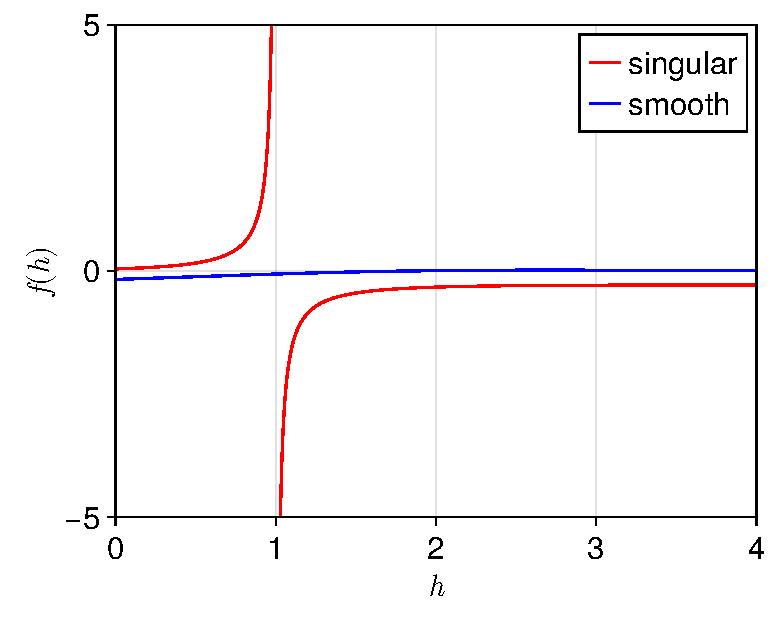
\includegraphics[width = 0.5\linewidth]{figs/fi.pdf}
    \caption{Split the integrand into smooth and singular parts.}
    \label{fig:split}
\end{figure}

An example is shown in Fig.~\ref{fig:split}, where we take~$a = b = H = k_0 = 1$.
For the smooth part, when~$k \to k_0$, both the numerator and denominator tends to zero so that
\begin{equation}
    \lim_{h \to h_0} \frac{J_0(bh) e^{- a h} - J_0(bh_0) e^{- a h_0}}{e^{- 2 H (h - h_0)} - 1}  = \lim_{h \to h_0} \frac{ \partial {J_0(bh) e^{- a h}}}{ \partial {e^{- 2 H (h - h_0)}}}\;,
\end{equation}
which is a finite value, and the integrand is a smooth function at~$h = h_0$.
When~$h \gg 1$, the smooth part is rapidly decaying, 
\begin{equation}
    \abs{\frac{J_0(bh) e^{- a h} - J_0(bh_0) e^{- a h_0}}{e^{- 2 H (h - h_0)} - 1} + J_0(bh_0) e^{- a h_0} } \to \abs{J_0(bh) e^{- a h}}\;,
\end{equation}
so that the integral can be directly evaluated using the same method as in the previous section, given by
\begin{equation}
    \int_0^{\infty} \to \int_0^{k_f}\;,
\end{equation}
since we have shown that the integrand is rapidly decaying, the truncation error can be estimated by
\begin{equation}
    E < \int_{k_f}^{\infty} \exp{(-a h)} dh < \frac{\exp{(-a h_f)}}{a}\;.
\end{equation}

Integral of the singular part can be calculated analytically, given by
\begin{equation}
    \begin{split}
        & \int_0^{\infty} \frac{J_0(bh_0) e^{- a h_0 - 2 H (h - h_0)}}{e^{- 2 H (h - h_0)} - 1} dh\\
        = & \frac{J_0(bh_0) e^{- a h_0}}{2H} \int_{0}^{\exp{(2 H h_0)}} \frac{1}{x - 1} dx\\
        = & \frac{J_0(bh_0) e^{- a h_0}}{2H} \ln{(\gamma_u \gamma_d - 1)}\;,
    \end{split}
\end{equation}
which is a finite value that can be easily calculated.

To verify the method above, we compared the result by the new approach shown above with a direct method given by
\begin{equation}
        I = \int_{0}^{2 h_0} \left[\frac{J_0(bh)e^{-ah}}{e^{-2H(h-h_0)} - 1} + \frac{J_0(bh_0)e^{-ah_0}}{2H(h - h_0)}\right] dh + \int_{2 h_0}^{\infty} \frac{J_0(bh)e^{-ah}}{e^{-2H(h-h_0)} - 1} dh\;.,\label{eq:direct}
\end{equation}
which directly subtracts the 1st order pole but take a high order of the Gaussian quadrature to reach high accuracy.

It is also shown that the integral converge much faster to the order of the quadrature.
We set~$a = b = k_0 = H = 1$, and $k_f = 10$,~$20$ and~$30$, the relative errors are shown in Fig.~\ref{fig:error} as functions of order of Gaussian quadrature, which shows that the error decay rapidly to desired accuracies.

\begin{figure}[htbp]
    \centering
    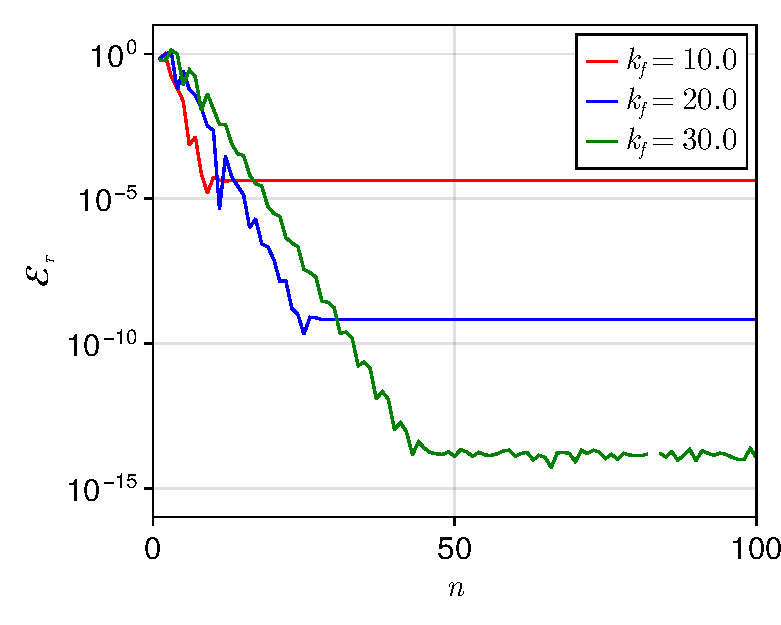
\includegraphics[width = 0.5\linewidth]{figs/int_convergence.pdf}
    \caption{Error to the order of the quadrature.}
    \label{fig:error}
\end{figure}

In summary, this approach provides an efficient method for handling the singularity in the short-range interaction by splitting the integrand into smooth and singular parts that can be evaluated separately with high accuracy.
This approach enables the simulation of negatively confined Coulomb systems with high accuracy and efficiency.

\section{Numerical results}
\label{sec:result}

In this section, we validate the accuracy and efficiency of our proposed method by applying it to several typical scientific problems, some the results are compared with that of the previously proposed method, such as the Ewald2D method, the image charge method and the HSMA method.
The runtime of QEM in one of the typical scenario is also tested.
These examples indicate that the proposed method is effective and efficient.
All calculations are performed in a Ubuntu system with AMD Ryzen Threadripper PRO 3995WX@2.2GHz, 1 CPU core.
Our software~\cite{QuasiEwald} is developed based on the Julia Programming Language~\cite{Julia-2017} and the open-source package \emph{CellListMap.jl}~\cite{celllistmap}.
The figures are generated by the open-source package \emph{Makie.jl}~\cite{DanischKrumbiegel2021}.

\begin{rmk}
    In this section, we focus on systems with positive permittivity, so that existing ICM-based methods can serve as reliable benchmarks. The numerical results for negatively confined systems will be presented in Section~\ref{sec::ssb}.
\end{rmk}

\subsection{Interaction between charges}

In this subsection, we validate the accuracy and convergence of our method by calculating the electrostatic interaction energy and force between charged particles distributed in quasi-2D systems.
It is remarked that the importance sampling technique is not applied here.

We first consider the electrostatic interaction between a pair of negatively charged particles, and the results are compared with that of the ICM-Ewald2D method.
We focused on two simple situations,~$\gamma_{d} = \gamma_{u} = \gamma = \pm 0.95$.
Size of the simulation box is set as~$(100, 100, 50)$, and the particle with charge~$+1$ is fixed at~$(50, 50, 1)$, while the other one with charge~$-1$ is moved along the $x$ axis or the $z$ axis.
For QEM, we set~$\alpha = 1.0$,~$n = 50$ and~$E = 4$.
The results are shown in Fig.~\ref{fig:E_xyz}, which indicates that QEM can accurately calculate the effects of the dielectric interface.

\begin{figure}[htb]
    \centering
    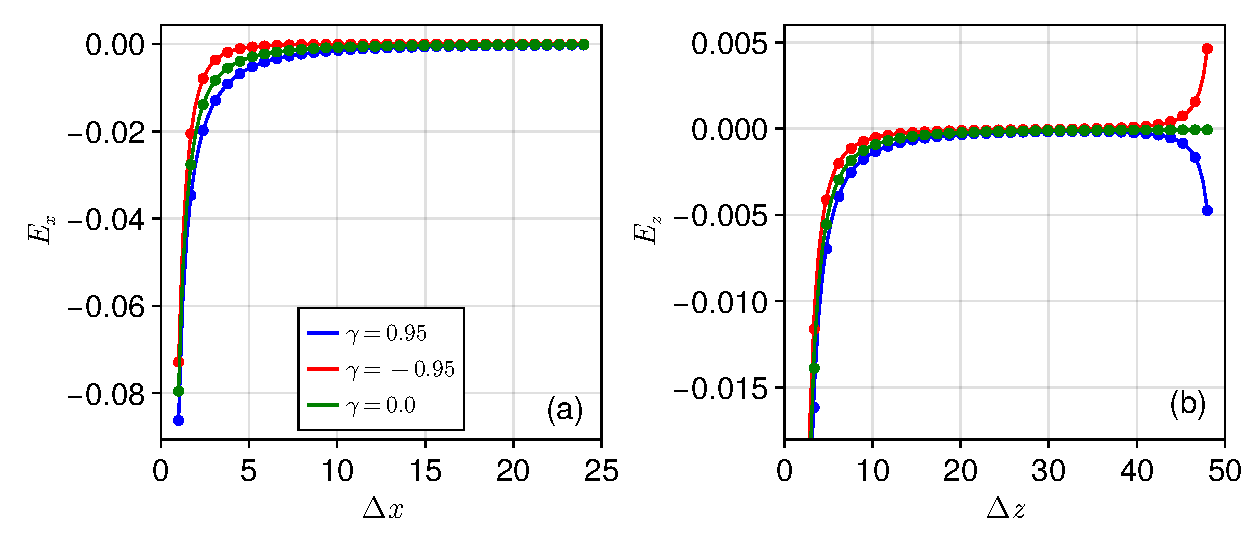
\includegraphics[width = \linewidth]{figs/E_xyz.pdf}
    \caption{
        Electric field in (a) $x$ and (b) $z$ between a pair of negatively charged particles, which are confined in a box with size of $(100, 100, 50)$.
        One of the particle is located at $(50, 50, 1)$, and the other one is located at (a) $(50 + \Delta x, 50, 1)$ and (b) $(50, 50, \Delta z)$.
        The lines are results by QEM and the dots are results by the ICM with direct lattice sum.
    }
    \label{fig:E_xyz}
\end{figure}

Then to validate the convergence of the QEM, we calculate the interaction energy of a system containing~$100$ randomly distributed particles using QEM, and the reference results are calculated by the ICM-Ewald2D method.
In Fig.~\ref{fig:Error_E}, the relative error of the interaction energy is plotted as function of the parameter~$E$ and the reflection rate~$\gamma$.
The results show that as $E$ increases, the relative error decreases rapidly, demonstrating the convergence of QEM.

\begin{figure}[htb]
    \centering
    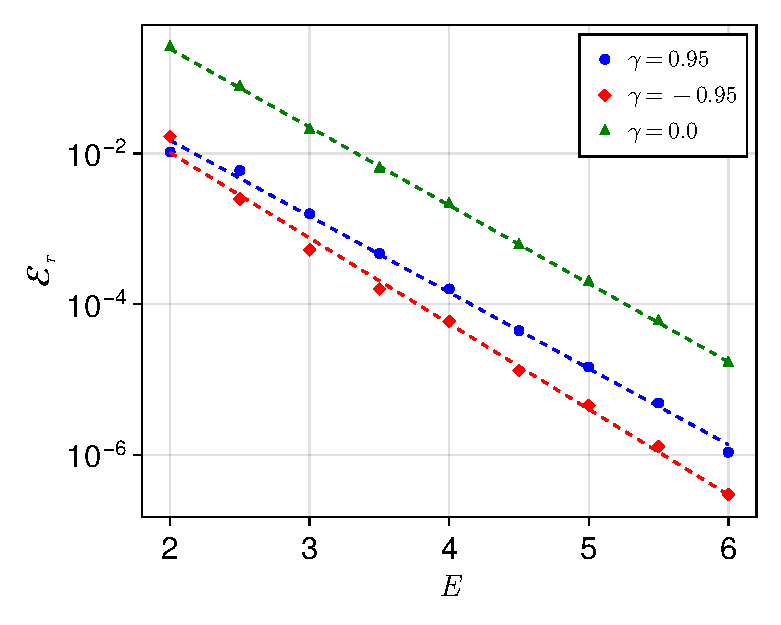
\includegraphics[width = 0.625\linewidth]{figs/e_total.pdf}
    \caption{
        Relative error of the energy of $100$ charged particles randomly distributed in a box with size of~$(100, 100, 50)$, as functions of the parameter~$E$ and reflection rates~$\gamma$.
    }
    \label{fig:Error_E}
\end{figure}


\subsection{Simulating electrolytes confined by dielectric interfaces}

To demonstrate the accuracy of the QEM for planar dielectric interfaces in a MD simulation, we study a few electrolytes modeled as the restricted primitive model, confined between two dielectric interfaces.
In all simulations, the box size is set as $(100 \tau_0, 100\tau_0, H)$, and consists of 436 particles immersed in continuum solvent characterized by a Bjerrum length $\ell_{\mathrm B} = e_0^2/(4 \pi \eps_c k_B T) = 3.5 \tau_0$, where~$e_0$ is the unit of smallest charge.
The ions are modeled as soft spheres of diameter~$\tau_0$ that have an excluded-volume interaction represented by a purely repulsive shifted-truncated Lennard-Jones (LJ) potential with energy scale~$\eps_{LJ} = k_B T$, where~$k_B$ is the Boltzmann constant and~$T$ is the absolute temperature.
The ions are confined by purely repulsive shifted-trunacted LJ walls ($\eps_\text{ion-wall} = k_B T$; $\tau_\text{ion-wall} = 0.5 \tau_0$) at $z = 0$ and $z = H$. 
The MD simulations is utilize a time step $0.001 t_0$, where $t_0 = \tau_0 m_0 / k_B T$ is the unit of time with $m_0 = 1$~(LJ unit), the ion mass, and temperature is controlled via Nosé–Hoover thermostat.
When evaluating the electrostatic interaction using the QEM, we set~$E = 4$,~$p = 30$ and~$n = 40$.
In all simulations, it takes~$2 \times 10^6$ time steps to reach equilibrium, after which we continue the simulation for $3 \times 10^6$ time steps for sampling.
We sample every 100 steps, which yields~$3 \times 10^{4}$ independent and equilibrated configurations.

\subsubsection{MD simulations of symmetric systems}

We first study symmetric systems where the top and bottom substrates have the same permittivity, i.e.,~$\gamma_u = \gamma_d = \gamma = \pm 0.95$, and we take~$H = 50 \tau_0$.
The system contains 218 cations and 218 anions carrying charge~$\pm e_0$, respectively.
To validate, we compared the charged distribution of QEM with result of the HSMA~\cite{liang2020harmonic}.
The ion density profiles by QEM and HSMA are shown in Fig.~\ref{fig:MD}, which shows that distributions obtained by QEM and HSMA overlap within statistical accuracy. 
The expected ion accumulation near high-permittivity surfaces and ion depletion near insulating interfaces are borne out by the simulations, which demonstrates that our method can accurately reproduce the characteristics of the system's equilibrium state.
The mean square displacements (MSD) in $xy$ and in $z$ of the simulation processes are shown in Fig.~\ref{fig:msd}.
The MSD in the periodic dimensions shown in Fig.~\ref{fig:msd}(a) is consistent with a normal diffusion process, where the~$O(t^2)$ and~$O(t)$ parts correspond to the short/long-time self diffusion, respectively.
Due to the confinements in~$z$, the MSD in the non-periodic dimension shown in Fig.~\ref{fig:msd}(b) behaves differently as a sub-diffusion process, where the MSD stop growing at long time, indicating the ions are confined by the dielectric interfaces.
The results here qualitatively agree well with that shown in previous experiments and simulations~\cite{das2010single, neusius2009subdiffusion}.

\begin{figure}[htbp]
    \centering
    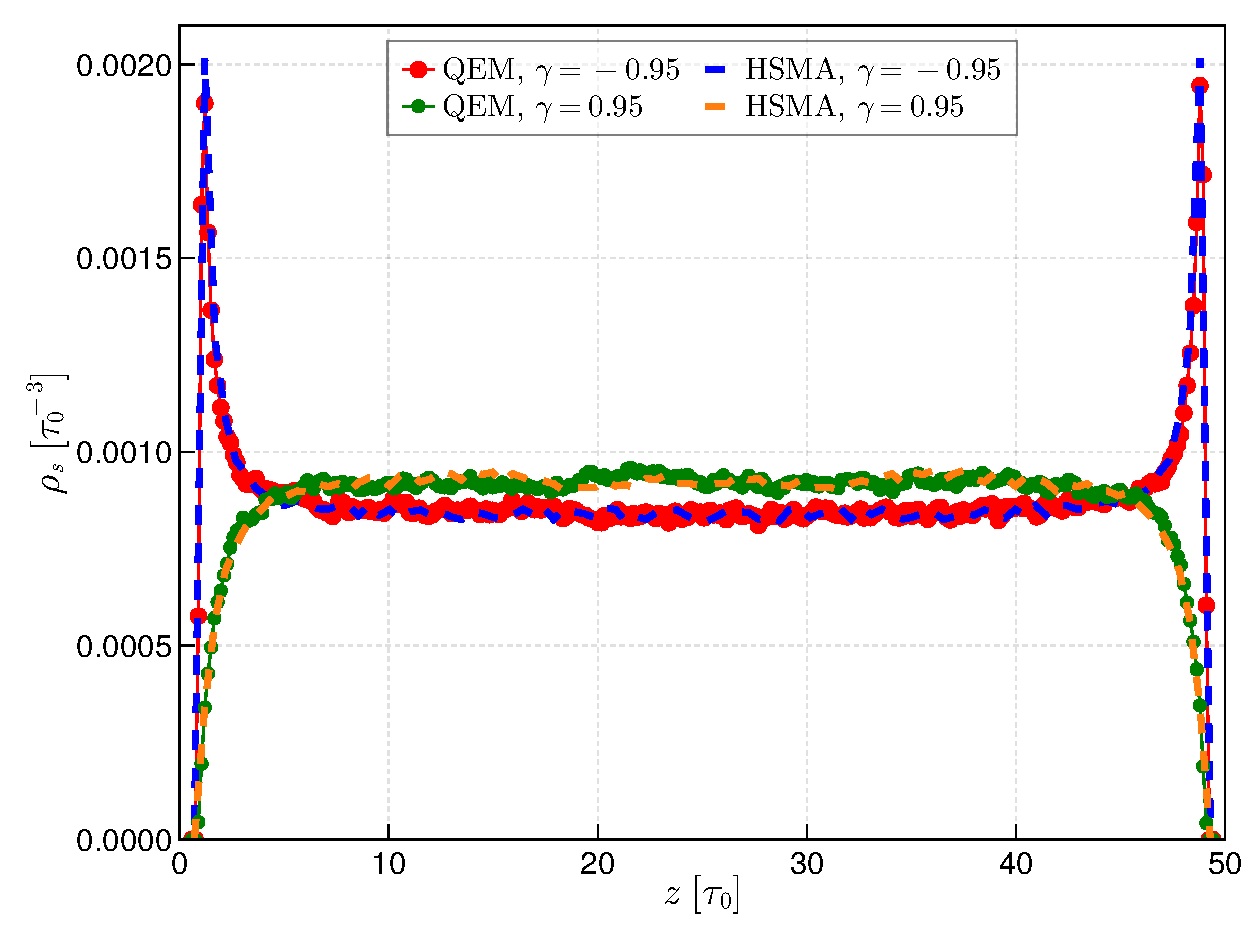
\includegraphics[width = 0.8 \linewidth]{figs/compare_HSMA.pdf}
    \caption{
        Distributions of ion density in~$z$ for symmetric electrolytes containing 218 cations and 218 anions and confined by neutral dielectric substrates with $\gamma_u = \gamma_d = \pm 0.95$ at~$z = 0$ and~$50\tau_0$, solid lines by QEM and dashed lines by HSMA.
    }
    \label{fig:MD}
\end{figure}

\begin{figure}[htbp]
    \centering
    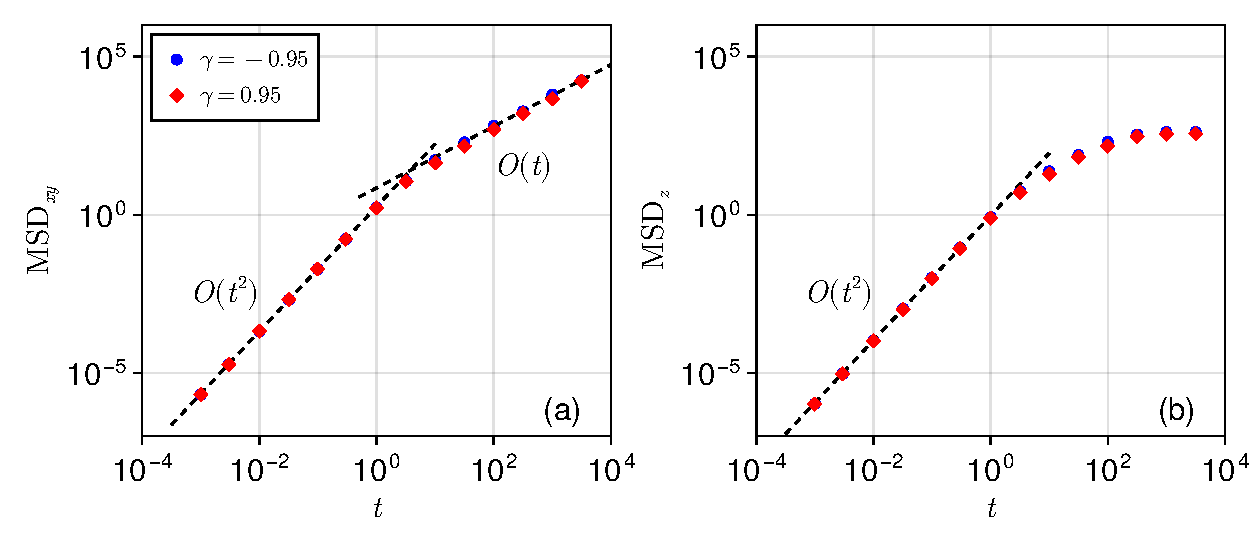
\includegraphics[width = 1.0 \linewidth]{figs/msd.pdf}
    \caption{
        The MSD of the ions in (a)~$xy$ and (b)~$z$, respectively, as functions of simulations time and reflection rates.
    }
    \label{fig:msd}
\end{figure}

Then CPU time for the QEM to compute the interactions between~$N$ particles is shown in Fig.~\ref{fig:timecost}, where cost of the Ewald2D method is also shown as reference.
The particle number surface density is fixed as~$4.36 \times 10^{-2} \tau_0^{-2}$ and thickness of the system is fixed to be~$50 \tau_0$, which are the same to the simulations above.
The number of charged particles is increased from~$10^2$ to~$10^5$.
For QEM, the same parameter as the previous simulations are applied; for Ewald2D method, parameter are selected so that the results are of 4-digit precision.
The results are shown in Fig.~\ref{fig:timecost}, which indicate that complexity of QEM is of~$\mathcal{O}(N)$.

\begin{figure}[htb]
    \centering
    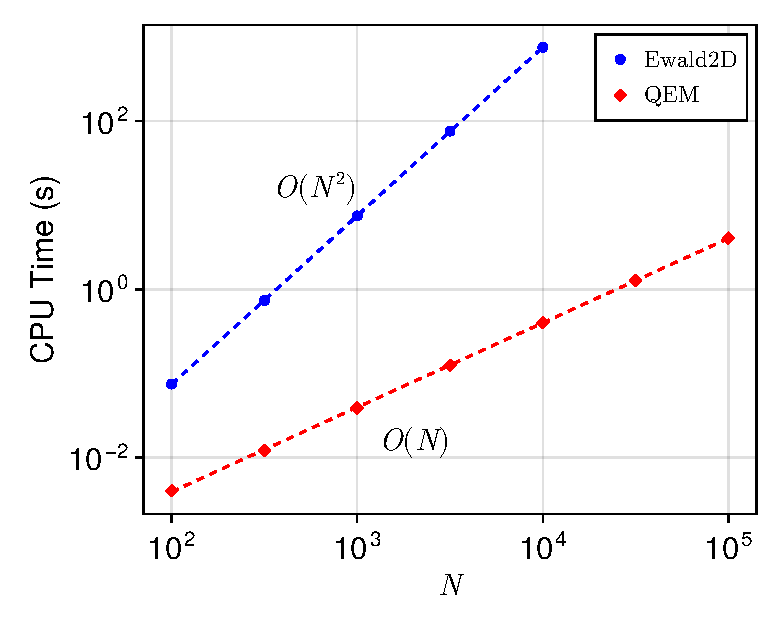
\includegraphics[width = 0.625\linewidth]{figs/runtime.pdf}
    \caption{
    CPU time of computing the interactions between all particles for different particle quantities under the condition of the same particle number surface density.
    The blue and red dots corresponding CPU time of Ewald2D method and QEM, and the dashed lines are fitted with slopes of~$2$ and~$1$, respectively.
    }
    \label{fig:timecost}
\end{figure}

\subsubsection{MD simulations of asymmetric systems}
As been mentioned above, QEM can be used to simulate asymmetric thin systems.
We consider two cases with asymmetry in dielectric mismatches and cation/anion valences.
In both cases, the thickness of the system is set as~$H = 10 \tau_0$, so that ~$L_{x/y} / H = 10$.

\textbf{Case I: Asymmetry in dielectric mismatches.}
In this case, we study the effect of the asymmetric dielectric mismatches.
The dielectric confinements are set as $\gamma_d = -0.95$ and~$\gamma_u = 0.95$, and the system contains 218 cations and 218 anions carrying charge~$\pm e_0$, respectively.
We keep other parameters the same as that of the previous example.

The spatial distribution of ions in~$z$ as shown in Fig.~\ref{fig:non_sym}.
Both cations and anions are attracted towards the lower dielectric plate with a negative reflection coefficient, while being repelled by the upper dielectric plate with a positive dielectric coefficient, thereby forming an strongly asymmetric spatial distribution as illustrated in Fig.~\ref{fig:non_sym}.

\begin{figure}[htb]
    \centering
    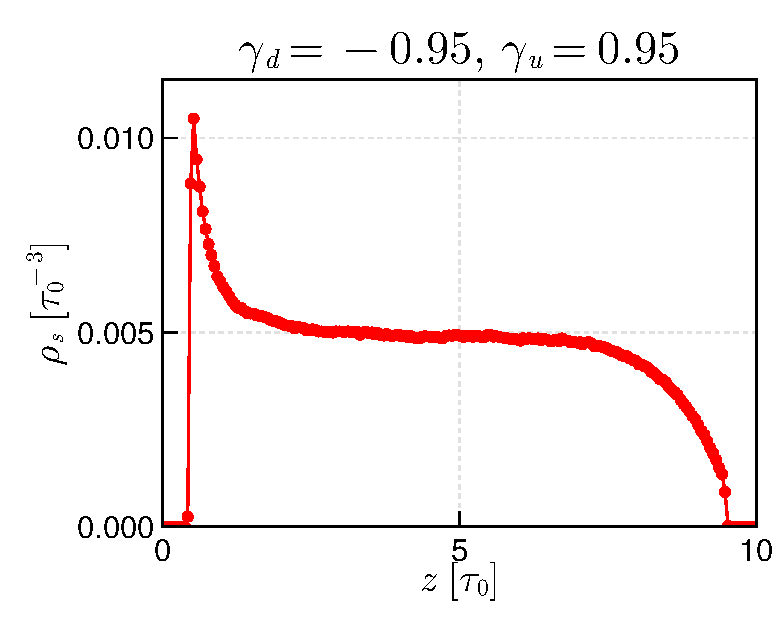
\includegraphics[width = 0.625\linewidth]{figs/non_symm.pdf}
    \caption{
        Ion density in~$z$ for symmetric electrolytes containing 218 cations and 218 anions and confined by neutral dielectric substrates with $\gamma_u = 0.95$,~$\gamma_d = -0.95$ at~$z = 0$ and~$10\tau_0$.
    }
    \label{fig:non_sym}
\end{figure}

\textbf{Case II: Asymmetry in cation/anion valences.}
Another application is the simulation of charge asymmetric systems.
In that simulation, we keep~$\gamma_u$ and $\gamma_d$ the same and equals to~$\gamma = \pm 0.95$, but simulate a $3:1$ salt with $109$ trivalent cations and $327$ monovalent anions. 
The other parameters are kept the same as above.

The results are shown in Fig.~\ref{fig:salt3-1}, which shows that the ion distributions are highly concentrated around the center or near the substrates.
For cations, due to the increase in the charge of the cations, the repulsive/attractive effects on both sides of the medium are significantly enhanced when~$\gamma$ greater or smaller than~$0$, respectively.
The anions are influenced by the distribution of cations, exhibiting characteristics of aggregation towards the center/sides, which are consistent with expectations.

\begin{figure}[htb]
  \centering
  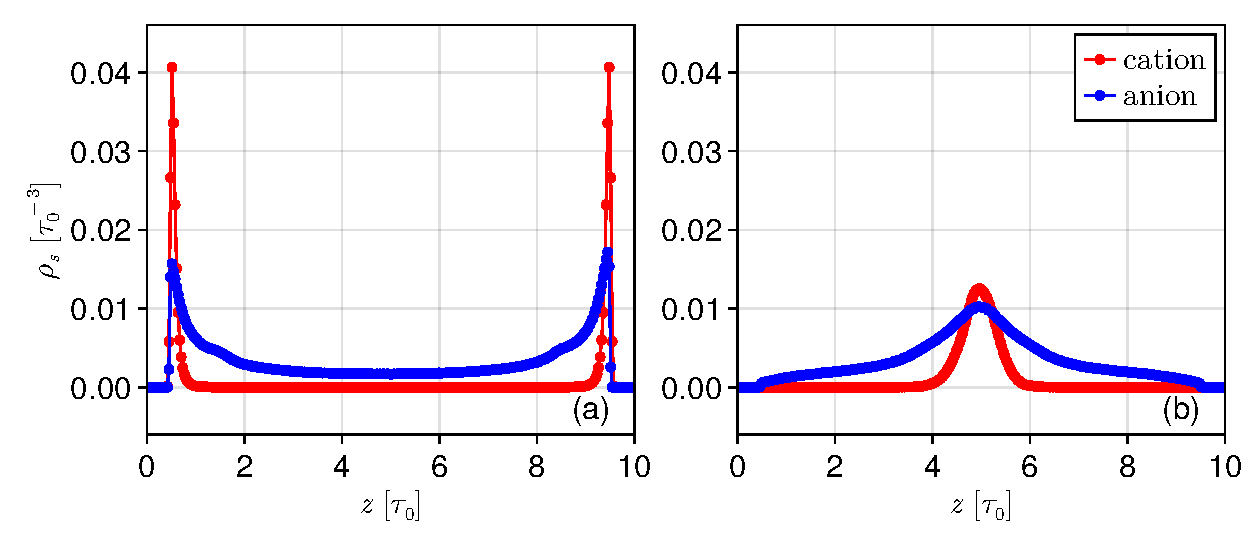
\includegraphics[width = \linewidth]{figs/density_3-1.pdf}

  \caption{
    Cation and anion density in~$z$ for a $3:1$ salt with $109$ trivalent cations and $327$ monovalent anions confined by neutral dielectric substrates with (a) $\gamma_u = \gamma_d = \gamma = - 0.95$ and (b) $\gamma_u = \gamma_d = \gamma = 0.95$.
    Red and blue lines are for cations and anions, respectively.
  }
    \label{fig:salt3-1}
\end{figure}

These cases indicates that QEM can also provide significant advantages in handling systems with particle asymmetry, thinness, and strong polarization effects.

\newpage

\chapter{Applications in Molecular Dynamics Simulations}
\label{chp_applications}
\section{Broken Symmetry in Quasi-2D Coulomb Systems}

\subsection{Oscillatory single particle field}

The dielectric confinement effect turns out to be physically fascinating even in the presence of a single charged particle. 
In Fig.~\ref{fig:force_x} (a), we present the electric field in the $x$ direction generated by a cation with valence~$\nu=1$ located at~$(x_0, y_0, \tau_0)$ in a quasi-2D system with a thickness of~$10\tau_0$, as a function of the distance from the cation~$\Delta x=x-x_0$, for different reflection rates~$\gamma$ characterizing the confinement. 
The field is defined as~$-\nu\ell_B\partial_x G(\mathbf{r}, \mathbf{r_0})$, where~$G(\mathbf{r}, \mathbf{r_0})$ is given by Eq.~\eqref{eq:G_pv}, and~$\ell_B=e_0^2/(4\pi\epsilon_0\epsilon k_B T)$ is the Bjerrum length of the solvent, with~$e_0$ the elementary charge,~$\epsilon_0$ the vacuum permittivity,~$k_B$ the Boltzmann constant, and~$T$ the temperature. 
For~$\vert\gamma\vert<1$ cases, as illustrated by the blue ($\gamma=-0.95$) and orange ($\gamma=0.95$) lines in Fig.~\ref{fig:force_x} (a), the polarization weakens or enhances the bare Coulomb field ($\gamma=0$), but with no qualitative difference. 
The results obtained by our method are in good agreement with those obtained by ICM, shown in dots in Fig.~\ref{fig:force_x} (a). 
However, for~$\vert\gamma\vert>1$, the results become non-trivial and qualitatively different. 
At short distance ($\tau_0<\Delta x < 10\tau_0$), we observe from Fig.~\ref{fig:force_x}(a) a continuous transition in the the near field interaction from like-charge attraction (LCA) into repulsion as~$\gamma$ increases from $-10$ to $+10$,
which can be understood as a significant enhancement of the polarization effect for~$\abs{\gamma}<1$ cases.
Even more interesting is the far field, it no longer decays monotonically but exhibits oscillatory behavior, which is rarely reported in previous studies.

\begin{figure}[htbp]
	\centering
	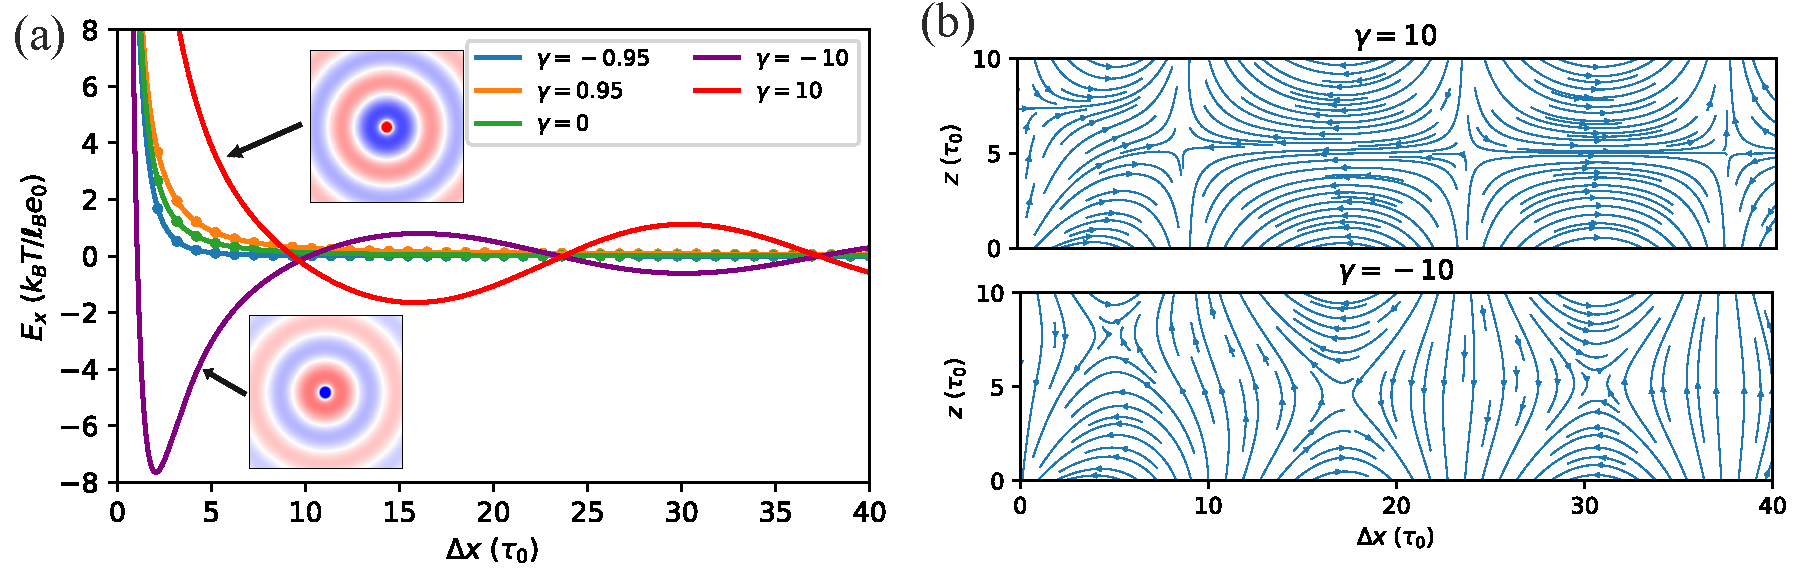
\includegraphics[width=0.45\textwidth]{figs/fig2.pdf}
	\caption{(a): the electric fields along~$x$ direction, generated by a cation with valence~$\nu=1$, fixed at~$z=\tau_0$, and confined by a pair of dielectric substrates located at~$z=0$ and~$10\tau_0$. Subplots depict the polarization charge density on the lower substrates. 
    (b): the corresponding field lines for the~$\gamma=\pm10$ scenarios.
		\label{fig:force_x}
            }
\end{figure}

To understand the origin of field oscillations, the polarization charge density profile on the substrate at~$z=0$ is shown in the subplots of Fig.~\ref{fig:force_x} (a). 
The charge density is defined by 
\begin{equation}
    \sigma(\V{r}) = \lim_{z \to 0^+} \nu \ell_B \eps_0  \left( 1 - \frac{\eps}{\eps'} \right) \partial_z G(\V{r}, \V{r_0})\;,
\end{equation}
and the field lines generated by $\sigma(\V r)$ are sketched in Fig.~\ref{fig:force_x} (b). 
The field oscillation is found to be generated by the strong transverse polarization charge density waves, influencing both the near and far fields. 
The oscillatory field lines has a very similar structure to that of a surface plasmonic resonance wave~\cite{willets2007localized}, but the physical origin is different. 
The oscillation is due to the reflected polarization enhanced by the dielectric confinement, characterized by parameters~$\gamma_1$,~$\gamma_2$, and~$L_z$. Particularly,
The confinement induced oscillation wave number is given by
\begin{equation}\label{eq:k0}
    k_0 = \frac{\ln{\gamma_1 \gamma_2}}{2 L_z}\;,
\end{equation}
which we will show analytically that this corresponds to a first-order pole in the Sommerfeld integral representation of the Green's function.
And the wavelength of the oscillation, defined as two times the distance between nearby zeros, satisfies 
\begin{equation}\label{eq:wavelength}
    \lambda \cdot k_0 = 2 \pi \;.
\end{equation}
Numerical validation shows that Eq.~\eqref{eq:wavelength} is highly robust under different choices of~$\V{r}$,~$\V{r}_0$,~$\gamma$, or~$L_z$, as shown in Fig.~\ref{fig:k_wavelegth}.
Importantly, the oscillation fields can be accurately predicted and controlled by adjusting~$k_0$. 
Eq.~\eqref{eq:k0} also indicates that the oscillation shall be weakened as $L_z$ is increased, and becomes non-oscillatory when $\gamma_1\gamma_2<1$.

\begin{figure}[htbp]
    \centering
    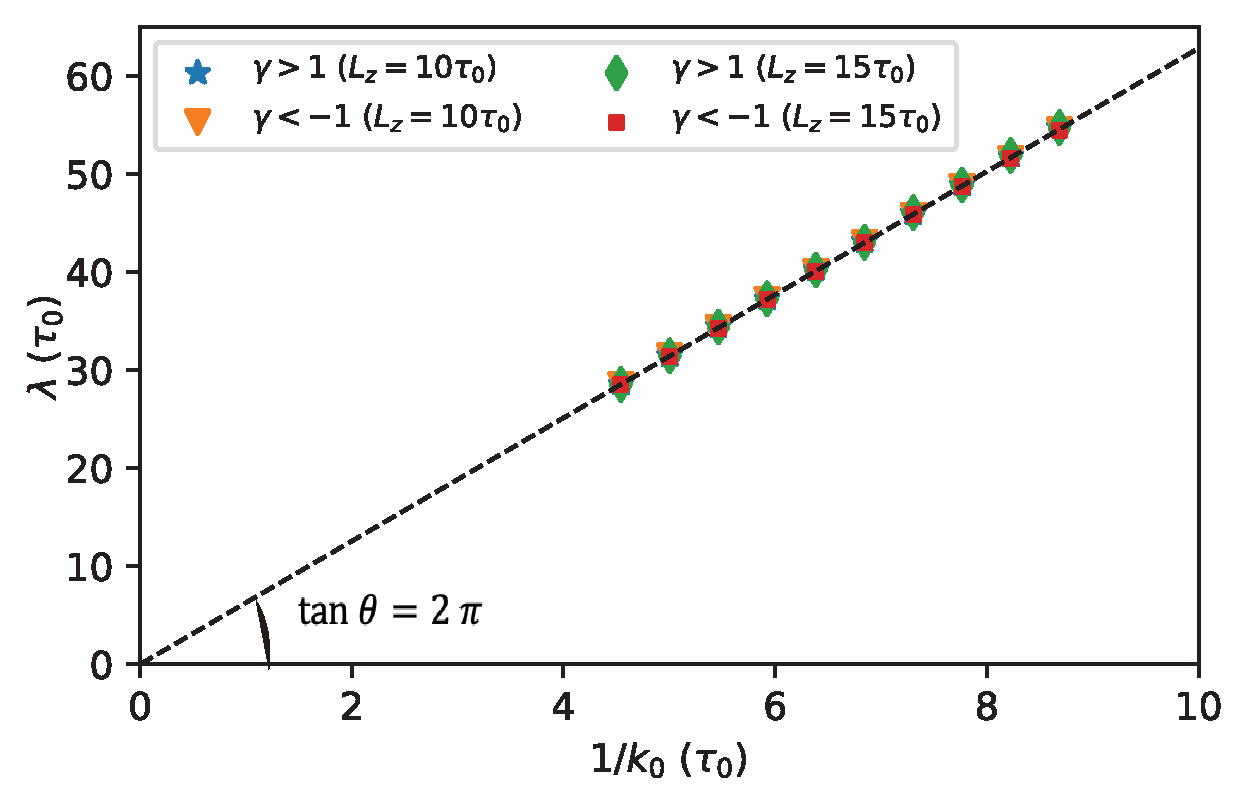
\includegraphics[width=0.6\textwidth]{figs/fig3.pdf}
    \caption{
        Numerical validations for the relationship between~$k_0$ and~$\lambda$ under various system parameter settings of~$\gamma$ and~$L_z$. For each case, $\lambda$ is approximated by averaging distances between nearby zeros of~$E_x$, and with different (randomly generated) locations in~$z$. 
    }
    \label{fig:k_wavelegth}
\end{figure}


\subsection{Theoretical origin for oscillations}

Eq.~\eqref{eq:G_point_charge} shows that the Green's function can be represented as a Sommerfeld integral, and the analytical form of $g(k, z, z_s)$ indicates that it has non-trival behaviors.
Clearly, $g(k, z, z_s)$ is divergent at $k=k_0$ (given in Eq.~\eqref{eq:k0}), and as $\gamma_1\gamma_2$ increases to be larger than 1, $k_0$ will shift onto the positive real axis, then the Sommerfeld integral needs to be renormalized.
Notice that when~$k \to k_0$, the divergent factor has the property
\begin{equation}
    \frac{1}{\gamma_1 \gamma_2 \exp{(-2 k L_z)} - 1} \to \frac{1}{2 L_z (k_0 - k)}\;,
\end{equation}
so that~$k_0$ is a first-order pole and the Cauchy principal value exists.
Then Eq.~\eqref{eq:G_point_charge} for~$\gamma_1 \gamma_2 > 1$ cases is given by
\begin{equation}\label{eq:G_pv}
    G(\V{r}, \V{s}) = - \text{p.v.} \left[ \int_{0}^{+\infty} 2 g(k, z, z_s) J_0(k \Delta \rho) k \text{d}k \right]  \;,
\end{equation}
which can be calculated numerically. In what follows, we analyze the oscillatory behavior~(for more details, see Supplementary Information (SI)~\cite{SI}). First, the Green's function consists of integrals of the following general form
\begin{equation}
    I_o = \int_0^{\infty} \frac{J_0(k \D \rho) \text{e}^{-ka}}{\exp{\left( 2 L_z (k_0 - k) \right)} - 1} \text{d}k\;,
\end{equation}
where~$\D \rho$,~$k_0$ and~$a$ are all positive constants.
We find that~$I_o$ can be further expanded as
\begin{equation}
    I_{o} = \frac{e^{-k_0 a}}{2L_z} \int_0^{\infty} \frac{J_0(k^\prime)}{k_0 \D \rho - k^\prime} \text{d}k^\prime + f(k_0, \D \rho, a),
\end{equation}
where~$k^\prime = k \D \rho$, and~$f(k_0, \D \rho, a)$ is a non-oscillatory analytic function which has minor contribution to~$I_o$.
The first integral term can be understood as a function of~$k_0 \D \rho$, or denoted as~$I_{m} (k_0 \D \rho)$. Clearly, $I_{m}$ is solely controlled by~$k_0$, given different parameters of $\gamma$ and $L_z$.
It is found that the first-order pole in $I_{m}$ provides the oscillatory mode, and we also numerical validated that the wavelength of the oscillation in $I_{m}$ indeed satisfies Eq.~\eqref{eq:wavelength}, which explains our findings.

\subsection{Spontaneous symmetry breaking in confined Coulomb systems}

To investigate the influence of dielectric nanoconfinement on the collective behavior of quasi-2D charged systems, we further developed a collection of numerical techniques to efficiently evaluate the Green's function Eq.~\eqref{eq:G_point_charge}. A novel Ewald-splitting type strategy is proposed, together with renormalization techniques and fast convergent quadrature schemes. All fine details and numerical validations are provided in the SI~\cite{SI}.
Our study focuses on a prototypical quasi-2D charged system, consisting of a binary mixture of charged particles described by the primitive model.
The system comprises~$N/2$ cations and~$N/2$ anions, each with the same diameter~$\tau_0$ and valence~$\pm 1$, resulting in an overall charge-neutral system. 
The Hamiltonian of the system is defined as follows, where~$i$ represents the~$i$-th particle with charge~$q_i$ located at position~$\V{r_i}$:
\begin{equation}
   \mathcal H = \frac{1}{2} \sum_{i,j=1}^{N}{}^\prime q_i q_j \ell_B G(\V r_i, \V r_j) + U_{\mathrm{LJ}}\;,\label{eq:Hamiltonian}
\end{equation}
The sum notation~$\sum_{i,j}{}^\prime$ implies that when~$i=j$, the function~$G(\V r, \V r)$ corresponds to the self-interaction term, and~$U_{\mathrm{LJ}}$ is the shift-truncated Lennard-Jones (LJ) potential energy used to model excluded-volume interactions. 
While this model disregards other important interactions observed in experimental realizations, it enables us to isolate the dielectric confinement effect. 
Similar systems have been studied recently in Refs.~\cite{dos2017simulations,liang2020harmonic,yuan2021particle}.

% two choices, 4 graphs or 3 graphs

\begin{figure}
	\centering
	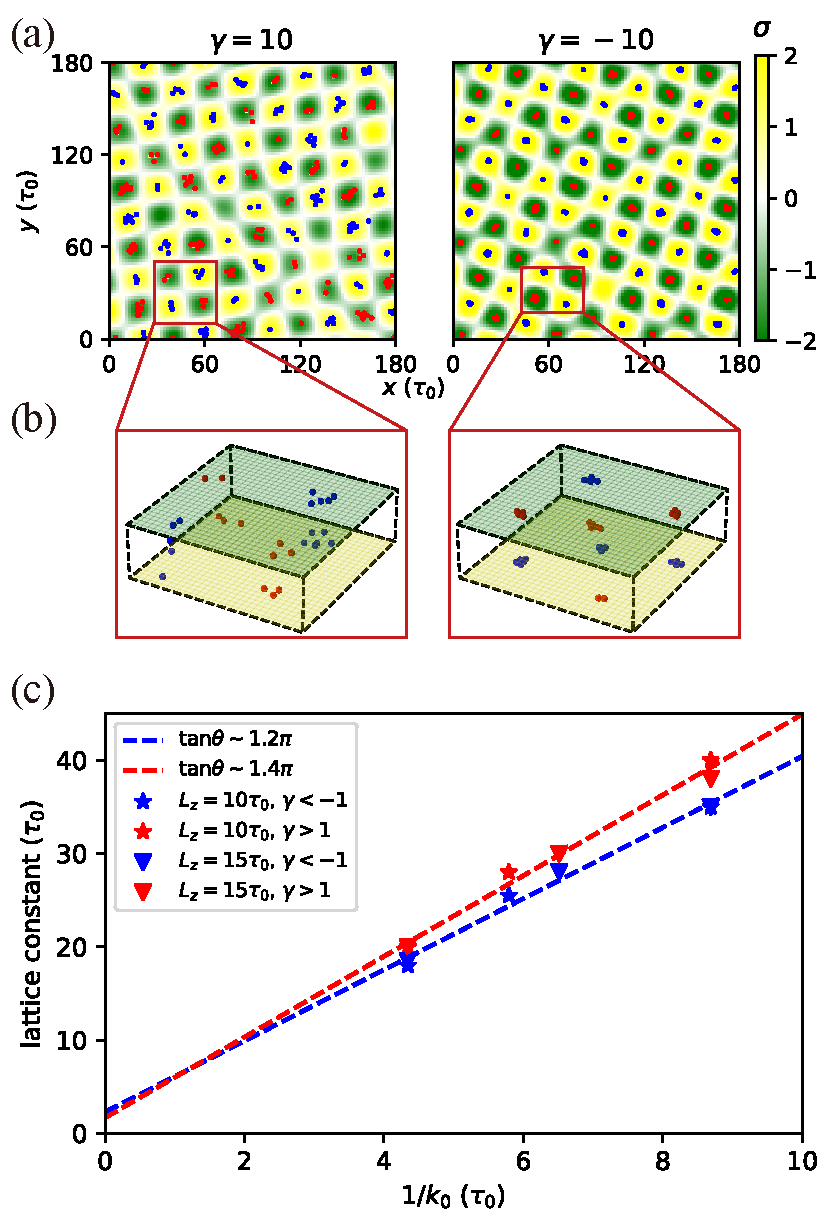
\includegraphics[width=0.43\textwidth]{figs/fig4.pdf}
	\caption{\label{fig:MD} 
        (a): Global particle distributions near the lower substrate and induced surface charge densities for~$\gamma = \pm 10$ and~$L_z = 10$. 
        Positive/negative induced surface charges are in yellow/green, while positive/negative particles are in red/blue, respectively.
        $\sigma$ unit:~$e_0/\tau_0^2$.
        (b): local 3D structures of the charged particles, enlarged from (a), while upper/lower boundaries are in green/yellow, respectively.
        (c): numerical validations for the relationship between the lattice constant and $k_0$. Symbols showing data points from individual simulations, dashed lines depict the linear fitted result.}
\end{figure}

In all the MD simulations, we maintain a constant box size in the~$xy$ plane of~$180\tau_0 \times 180\tau_0$, which is confirmed to eliminate boundary effects.
We vary the values of~$L_z$ and~$\gamma$ to adjust the wave number~$k_0$. 
The system contains~$300$ cations and~$300$ anions.
To isolate electrostatic effect, the reduced temperature $T_r$ is defined as~$T_r =k_{\mathrm B}T/\varepsilon_{\mathrm{Coul}}$, where~$\varepsilon_{\mathrm{Coul}} = e_0^2/(4 \pi \eps (3.5 \tau_0))$ and we set~$\varepsilon_{\mathrm{LJ}} = k_B T$ for both particle-particle and particle-substrate interactions. 
We integrate the temporal evolution using the Velocity-Verlet algorithm and control the temperature using the Anderson thermostat with stochastic collision frequency~$\omega = 0.1$ and reduced temperature~$T_r = 1$.

In the $\abs{\gamma}\leq 1$ regime, extensive simulation works have been done recently~\cite{liang2020harmonic,yuan2021particle} and no SSB phenomenon has been found, i.e., the density distributions of cations $\rho_{+}(\V r)$ and anions $\rho_{-}(\V r)$  always maintain symmetries of the system, given by 1) \emph{cross symmetry} in the confined space: $\rho_{+}(\V r)=\rho_{-}(\V r)$, 2) \emph{longitudinal symmetry}: $\rho_{\pm}(x,y,z)=\rho_{\pm}(x,y,L_z-z)$, and 3) \emph{transverse symmetry}: $\rho_{\pm}(x,y,z)=\rho_{\pm}(x',y',z)$. 
Our simulations give symmetric results for  $\abs{\gamma}\leq 1$, consistent as previous investigations (details are documented in SI~\cite{SI}). 
In the following discussions we will focus on the strongly polarizable cases of $\abs{\gamma}>1$, where SSB phenomena arise.

Fig.~\ref{fig:MD}(a) shows two snapshots for particle distributions near the lower substrate and the corresponding induced surface charge densities, for $\gamma=\pm10$ and $L_z=10$. It clearly shows, for the first time, SSB phenomena in such dielectric confined charged system: both the cross and transverse symmetries are broken when $\gamma=10$; and the remaining longitudinal symmetry is further broken when $\gamma=-10$ (as shown in Fig.~\ref{fig:MD}(b)).

Globally, we observe charged particles spontaneously forming square lattice structures near the substrates for both~$\gamma > 1$ and~$\gamma < -1$ cases, which breaks the transverse symmetry. 
We attribute this to the long-range single particle oscillatory field in the $xy$-plane, which directs particles self-organizing into a \emph{checkerboard} structure, so as to enhance the overall induced charge landscape, which helps confining particles in local potential wells.
Locally within each lattice site, two different particle structures are observed: for~$\gamma >1$, interfacial liquid phase is formed, while for~$\gamma < -1$, likely-charged particles self-assemble into 2D clusters, both can be understood by the near field behaviors due to a single confined particle, as was discussed and illustrated in Fig.~\ref{fig:force_x} (a).

Interestingly, in the longitudinal direction, we find that the interfacial liquids/clusters on opposing substrates are strongly correlated, i.e., there is a one-to-one “pairing” between the opposing particle structures, as show in Fig.~\ref{fig:MD}(b).
For $\gamma=10$, the longitudinal pairing is between symmetrically charged particles; while for $\gamma=-10$, the pairing becomes anti-symmetric, which further breaks the longitudinal symmetry. The symmetric/anti-symmetric longitudinal paring is due to the induced charge landscape on opposing substrates, it is clearly that for $\gamma=10$, the checkerboard structures would be matched symmetrically, while for $\gamma=-10$ a negative sign is added to the reflection rates, forming anti-symmetric pairs.

Finally, it is worth noting that the formed square lattices can be well-controlled via the single parameter~$k_0$, consistent with our theoretical prediction.
As shown in Figure \ref{fig:MD}(c), the lattice constant of the system is found to be proportional to $k_0^{-1}$, with various choice of $L_z$ and $\gamma$. 
Two slightly different linear relationships are observed, with fitted ratio~$1.2 \pi$ and~$1.4 \pi$ for~$\gamma < -1$ and~$\gamma > 1$ cases, respectively. 
The distance between neighboring clusters is found to be consistent with the second zero point of the induced surface charge density profile due to a single point charge (see subplots of Fig.~\ref{fig:force_x} (a)). The mechanism allows one to efficiently modulate the collective phase of dielectric confined systems.
\newpage

\chapter{Conclusions}
\label{chp_conclusion}
Quasi-2D systems are ubiquitous in nature and play a crucial role in various fields, including materials science, biophysics, and electrochemistry. 
However, the simulation of quasi-2D systems is challenging due to the long-range Coulomb interactions and the complex boundary conditions.
The challenges can be summarized as follows:
\begin{itemize}
    \item[1.] The reduced symmetry of the system leads to the breakdown of the traditional Ewald summation, especially for the systems with large aspect ratios.
    \item[2.] The dielectric confinement introduces additional complexity to the system, which requires careful treatment of the polarization effect, especially for the systems with strong polarizable interfaces.
    % \item[3.] The large system size and the need for high accuracy pose significant challenges for the computational resources.
\end{itemize}
Due to these challenges, existing methods are largely restricted to quasi-2D systems with moderate aspect ratios and weakly polarizable interfaces, limiting their broader applicability.
Aiming to develop a general and efficient simulation framework for quasi-2D Coulomb systems, we systematically study the confined quasi-2D Coulomb systems in this thesis, including theoretical analysis, numerical methods and applications.

For the theoretical part, we presented a rigorous error analysis of Ewald summation for dielectric-confined planar systems, where the polarization potential and force field are modeled using an infinitely reflected image charge series. 
In particular, we address the truncation error of the image charge series and the error estimations associated with the ELC term involving image charges, which may introduce significant errors but are often over-looked.
Our error estimations are validated numerically across several prototypical systems. Moreover, through analysis, we are able to elucidate the counterintuitive non-monotonic error behavior observed in previous simulation studies.
Based on the theoretical insights, we propose an optimal parameter selection strategy, offering practical guidance for achieving efficient and accurate MD simulations the confined systems.

For the numerical part, we have developed a class of novel fast algorithms for simulating quasi-2D Coulomb systems, making significant methodological advances in computational physics. 
These methods are summarized as follows:

For confined Coulomb systems, our approach (SOEwald2D) connects Ewald splitting with a sum-of-exponentials (SOE) approximation, which ensures uniform convergence along the whole non-periodic dimension. 
We further incorporate importance sampling in Fourier space over the periodic dimensions, achieving an overall $O(N)$ simulation complexity. 
The algorithm has distinct features over the other existing approaches:
\begin{itemize}
	\item[1.] Our approach provides a well-defined computational model for both discrete free-ions and continuous surface charge densities, and is consistent under both NVT and NPT ensembles.
	\item[2.] The simulation algorithm has linear complexity with small prefactor, and it does not depend on either FFT or FMM for its asymptotic complexity.
	\item[3.] Instead of modifying FFT and FMM-based methods, which are originally proposed for periodic/free-space systems, our scheme is tailored for partially-periodic systems, it perfectly handles the anisotropy of such systems without any loss of efficiency.
	\item[4.] Our method is mesh free, and can be flexibly extended to other partially-periodic lattice kernel summations in arbitrary dimensions, thanks to the SOE approximation and random batch sampling method.
\end{itemize}

For dielectrically confined Coulomb systems, we have developed a novel algorithm called the random batch Ewald2D (RBE2D) method, which is able to handle the dielectric interfaces very efficiently.
We first present the reformulation for the quasi-2D Ewald sum into a Ewald3D sum with an ELC term and an infinite boundary correction (IBC) term. Rigorous error analysis is also presented, justifying the optimal parameter choices for a given accuracy.
Then RBE is applied to achieve $O(N)$ complexity: the stochastic approximation has reduced variances thanks to an importance sampling strategy and coupling with a proper thermostat in MD simulations.
For systems with dielectric mismatch, the subtle dielectric interface problem is reduced to a homogeneous problem via image charge reflection,
we further recalibrate the structure factor coefficients for the image series in $\V k$-space, 
enabling the computation of the polarization contributions with minimal overhead. 
The main advantage of our method compared with existing methods is twofold: 
\begin{itemize}
	\item[1.] Our method relies on a random batch sampling strategy in $\V k$-space to achieve linear-scaling, thus it is highly efficient and has strong scalability.
	\item[2.] Our method is mesh-free, and can be applied to strongly confined systems with negligible extra cost.
\end{itemize}

For negatively charged systems, we have developed a novel method called the quasi-Ewald method (QEM).
We first propose a new splitting scheme different from the traditional Ewald splitting, and then derive the QEM based on the new splitting scheme and an analytical expression for the interaction potential.
For both short-range and long-range interactions, efficient and accurate algorithms are carefully derived, and with the help of RBE, the QEM is able to achieve linear-scaling in both CPU and memory consumptions.
We further proposed a singularity subraction scheme to handle the divergence problem induced by the strongly polarizable interfaces, and extend the QEM to systems with negatively dielectric confinements.
The QEM is the first method that can properly handle the divergence problem induced by the strongly polarizable interfaces and achieve linear-scaling.


In general, our methods are mesh free and can reach the optimal $O(N)$ complexity in both CPU and memory consumptions without relying on either FFT or FMM, and are able to handle the anisotropy of the system.
Both analysis and numerical results validate that our method is not affected by the aspect ratio of the system.
These advantages make our method a powerful tool for simulating quasi-2D Coulomb systems, and it is expected to have broad applications in various fields.

For the application part, we have applied our methods to the simulation of all-atom water models confined by slabs, and the results are in good agreement with the experimental and theoretical results, demonstrating the accuracy and efficiency of our methods.
We also applied our methods to the simulation of negatively confined quasi-2D systems, and observed spontaneous symmetry broken solely via dielectric confinements for the first time.
These applications showcase the potential of our methods to provide new insights into the physics of quasi-2D systems.

Despite the advances made, our theoretical analysis and numerical methods have several limitations that warrant discussion.
First, our framework relies on the assumption of planar substrates with uniform dielectric constants.
This restricts its applicability to real-world systems where surfaces often exhibit complex geometries and spatially varying dielectric properties.
Second, while our work focuses on point charge interactions, many physical systems involve polarizable particles with complex shapes and charge distributions.
These characteristics can give rise to fascinating phenomena such as like-charge attraction, self-assembly, and phase separation - scenarios where our current methods cannot be directly applied.
Third, the mathematical properties of our proposed methods, particularly regarding strong convergence and ergodicity, remain incompletely understood and represent important open problems in the field.
These limitations constrain the broader applicability of our methods and represent critical areas for future investigation and methodological advancement.


Looking ahead, we envision two key directions for future research as follows.

The first direction is to extend our methods to more complex systems, including systems with complex geometries such as curved surfaces and polarizable particles.
In such cases, we anticipate that a boundary integral formulation can be incorporated -- the polarization effect can be approximated as the field due to induced surface charges, then in each field evaluations, the proposed methods may be applied to reduce the computational cost, so that it will be capable of efficiently and accurately simulate charged particles confined by structured surfaces~\cite{wu2018asymmetric}.

The second direction is to extend our methods to different interaction kernels, such as the dipolar interactions~\cite{Messina2017PRL}, the Stokes interactions~\cite{barnett2018unified} and the Yukawa interactions~\cite{Hou2009PRL}, which plays important roles in many physical systems.
These kernels are also long-ranged and have more complex behaviors.
More interestingly, the recently proposed machine learning interaction potential~\cite{cheng2025latent, ji2025machinelearninginteratomicpotentialslongrange} for long-range systems can be consider as a special type of kernel, and it is expected to be a powerful tool for simulating complex systems.
It is challenging to extend our methods to these kernels, and it is also an interesting direction for future research.

While these research directions present significant theoretical and computational challenges, we believe the potential impact on our understanding of confined charged systems makes them compelling areas for future investigation.
\newpage

%%%%%%%%%%%%%%%%%%%%%%%%%%%%%%%%%%%%%%%%%%%%%%%%%%%%%%%%%%%%%%%%%%%%%%%%%
%                                                                       %
%      9) BIBLIOGRAPHY                                                  %
%                                                                       %
% This example uses bibtex to generate the required Bibliography. Refer %
% to the % the file ustthesis_test.bib for the entries of the           %
% Bibliography. Note that only the cited entries are printed.           %
%                                                                       %
% If BibTeX is not used to typeset the bibliography, replace the        %
% following line with the \begin{thebibliography} and \end{bibliography}%
% commands (the "thebibliography" environment) to process the           %
% Bibliography.                                                         %
%                                                                       %
%%%%%%%%%%%%%%%%%%%%%%%%%%%%%%%%%%%%%%%%%%%%%%%%%%%%%%%%%%%%%%%%%%%%%%%%%

%%%%%%%%%%%%%%%%%%%%%%%%%%%%%%%%%%%%%%%%%%%%%%%%%%%%%%%%%%%%%%%%%%%%%%%%%
%                                                                       %
% The recommended bibliography style is the IEEE bibliography style.    %
% "ustbib" defines the IEEE bibliography standard with the added        %
% ability of sorting the items by name of author.                       %
%                                                                       %
% If you are not using BibTeX to process your Bibliography, comment out %
% the following line.                                                   %
%                                                                       %
%%%%%%%%%%%%%%%%%%%%%%%%%%%%%%%%%%%%%%%%%%%%%%%%%%%%%%%%%%%%%%%%%%%%%%%%%

\addcontentsline{toc}{chapter}{Bibliography}
\bibliographystyle{elsart-num-sort}
\bibliography{references}
\newpage

%%%%%%%%%%%%%%%%%%%%%%%%%%%%%%%%%%%%%%%%%%%%%%%%%%%%%%%%%%%%%%%%%%%%%%%%%
%                                                                       %
%     10) APPENDIX (If Any)                                              %
%                                                                       %
% \appendix command marks the beginning of the APPENDIX part of the     %
% Thesis. The usual \chapter command is used for the different chapters %
% of the Appendix.                                                      %
%                                                                       %
%%%%%%%%%%%%%%%%%%%%%%%%%%%%%%%%%%%%%%%%%%%%%%%%%%%%%%%%%%%%%%%%%%%%%%%%%
\appendix

\chapter{Supplementary Mathematical Background}
\label{chp_math}
\section{Fundamental results from Fourier analysis} \label{app::Fourier}
In this appendix, we state several fundamental results from Fourier analysis for doubly periodic functions, associated with the Fourier transform pair defined in Definition~\ref{Def::Fourier}. These results are useful for us, and their proofs are well established and can be referenced in classical literature, such as in the work of Stein and Shakarchi~\cite{stein2011fourier}.
\begin{lem}\label{lem::Convolution}
	(Convolution theorem) Let $f(\bm{\rho},z)$ and $g(\bm{\rho},z)$ be two functions which are periodic in $\bm{\rho}$ and non-periodic in $z$. Suppose that $f$ and $g$ have Fourier transform $\widetilde{f}$ and $\widetilde{g}$, respectively. Their convolution is defined by
	\begin{equation}\label{eq:Q2D_cov}
		u(\bm{\rho},z):=(f\ast g)(\bm{\rho},z)=\int_{\mathcal{R}^2}\int_{\mathbb{R}}f(\bm{\rho}-\bm{\rho}',z-z')g(\bm{\rho}',z')dz'd\bm{\rho}',
	\end{equation}
	satisfying
	\begin{equation}
		\widetilde{u}(\bm{k},\kappa)=\widetilde{f}(\bm{k},\kappa)\widetilde{g}(\bm{k},\kappa).
	\end{equation}
	
\end{lem}
\begin{lem}\label{lem::Poisson}
	(Poisson summation formula) Let $f(\bm{\rho},z)$ be a function which is periodic in $\bm{\rho}$ and non-periodic in $z$. Suppose that $f$ has Fourier transform $\widetilde{f}$ and $\bm{r}=(\bm{\rho},z)$. Then one has
	\begin{equation}
		\sum_{\bm{m}\in \mathbb{Z}^2} f(\bm{r} + \V{\mathcal{M}}) = \frac{1}{2\pi L_x L_y}\sum_{\bm{k}\in \mathcal{K}^2}\int_{\mathbb{R}}\widetilde{f}(\bm{k},\kappa)e^{\m{i} \bm{k}\cdot\bm{\rho}}e^{\m{i} \kappa z}d\kappa.
	\end{equation}
\end{lem}
\begin{lem}\label{lem::2dfourier}
	(Radially symmetric functions) 
	Suppose that $f(\rho,z)$ is periodic and radially symmetric in $\bm{\rho}$, i.e., $f(\bm{\rho},z)=f(\rho,z)$. Then its Fourier transform $\widetilde{f}$ is also radially symmetric. Indeed, one has
	\begin{equation}
		\widetilde{f}(\rho,z)=2\pi\int_{0}^{\infty}J_0(k\rho)f(\rho,z)\rho d\rho.
	\end{equation}
\end{lem}

\section{Quadrature error of the trapezoidal rule}\label{app::trapezoidal}
We employ the method of contour integrals~\cite{Donaldson1972SINUA,trefethen2014Rev} to derive a precise estimation for the error in  {the} trapezoidal rule when discretizing Eqs.~\eqref{eq:ewald2d-intform1} and \eqref{eq::J02}. Consider the integral
\begin{equation}\label{eq::A.1}
I=\int_{-\infty}^{\infty }\frac{e^{-(a^2+t^2)}}{a^2+t^2}e^{\i b t}dt,
\end{equation}
where $a\geq 0$ and $b\in\mathbb{R}$. We approximate $I$ using a $(2M+1)$-point trapezoidal rule:
\begin{equation}
I_{M,\xi}=\xi\sum_{j=-M}^{M}\frac{e^{-a^2-(j\xi)^2}}{a^2+(j\xi)^2}e^{\i b j\xi},
\end{equation}
where $\xi>0$ is the step size, and we define the remainder as $E_{M,\xi}:=I-I_{M,\xi}$. Note that the integrand of $I$ has two simple poles at $t_{\pm}=\pm \i a$. Let $\Gamma_{\pm}$ be two positively/negatively oriented rectangular contours with vertices $(M+1/2)\xi\pm\i a^*$, $-(M+1/2)\xi\pm\i a^*$, $(M+1/2)\xi$, and $-(M+1/2)\xi$ (see Fig.~\ref{fig:Trapezoidal}). We enforce $a^*>a$ so that $\Gamma_{\pm}$ encloses both the interval $[-M \xi,M \xi]$ and the pole $t_{\pm}$. By following the approach given in~\cite{Donaldson1972SINUA} and applying Cauchy's theorem, we can derive an estimate for $E_{M,\xi}$ in the limit $M\rightarrow \infty$:
\begin{equation}
E_{M,\xi}=\int_{\Gamma_++\Gamma_-}\frac{e^{-(a^2+t^2)+\i b t}}{a^2+t^2}\varphi(t)dt-2\pi\i \text{Res}\left[\frac{e^{-(a^2+t^2)+\i b t}}{a^2+t^2}\varphi(t),\pm \i a\right],
\end{equation}
where
\begin{align}
\varphi(t)=\begin{cases}
\dfrac{1}{1-e^{2\pi\i t/\xi}},\,\quad &\text{Im}(t)<0,\\[1em]
-\dfrac{1}{1-e^{-2\pi\i t/\xi}},\,\quad&\text{Im}(t)>0,
\end{cases}
\end{align}
is related to the characteristic function of the trapezoidal rule, and $\text{Res}[f(t),t_0]$ denotes the residue of a function $f$ at a pole $t_0$. Since the contributions from the vertical sides of $\Gamma_{\pm}$ vanish in the limit $M\rightarrow \infty$ and by using residue calculus, we have
\begin{equation}\label{eq::A.5}
E_{M,\xi}=\left(\int_{-\infty+\i a^*}^{\infty+\i a^*}-\int_{-\infty-\i a^*}^{\infty-\i a^*}\right)\frac{e^{-(a^2+t^2)+\i b t}}{a^2+t^2}\varphi(t)dt+\frac{\pi}{a}\frac{e^{-ab}+e^{ab}}{1-e^{2\pi a/\xi}}.
\end{equation}
In Eq.~\eqref{eq::A.5}, the last term can be considered as the residue correction of the rule, while the remainder integral along $\text{Im}(t)=a^*$ can be estimated as
\begin{equation}
\begin{split}
\left|\int_{-\infty+\i a^*}^{\infty+\i a^*}\frac{e^{-(a^2+t^2)+\i b t}}{a^2+t^2}\varphi(t)dt\right|&\leq e^{(a^*)^2-a^2-a^*b-2\pi a^*/\xi}\int_{-\infty}^{\infty}\frac{|a^2+(t+\i a^*)^2|^{-1}e^{-t^2}}{\left|1-e^{2\pi\i t/\xi-2\pi a^*/\xi}\right|}dt\\
&\leq\frac{\sqrt{\pi}e^{(a^*)^2-a^2-a^*b-2\pi a^*/\xi}}{(a^*)^2-a^2}.
\end{split}
\end{equation}

To obtain a closed formula, it is necessary to determine the extremum of the exponent under the condition $a^*>a>0$. Since the range of $a$ is not specified, we can safely choose $a^*=\pi/\xi+b/2$ if $\pi/\xi+b/2>a$, and $a^*=\sqrt{a^2+1}$ otherwise. This choice ensures a decay rate of at least $\sim O(e^{-\text{sign}(\pi/\xi+b/2)|\pi/\xi+b/2|^2})$, where $\text{sign}(t)=1$ if $t> 0$, $\text{sign}(t)=0$ if $t=0$, and $\text{sign}(t)=-1$ otherwise. By following a similar procedure, we can derive that the integral along $\text{Im}(t)=-a^*$ in Eq.~\eqref{eq::A.5} decays with order $O(e^{-\text{sign}(\pi/\xi-b/2)|\pi/\xi-b/2|^2})$. Consequently, we can conclude that
\begin{equation}
E_{M,\xi}=\frac{\pi}{a}\frac{e^{-ab}+e^{ab}}{1-e^{2\pi a/\xi}}+E_{\text{err}},
\end{equation}
where the remainder error term can be estimated as 
\begin{equation}\label{eq::A.8}
|E_{\text{err}}|\sim O(e^{-\text{sign}(\pi/\xi-|b|/2)\left|\pi/\xi-|b|/2\right|^2}).
\end{equation}

\begin{figure}[!ht]
    \begin{center}
    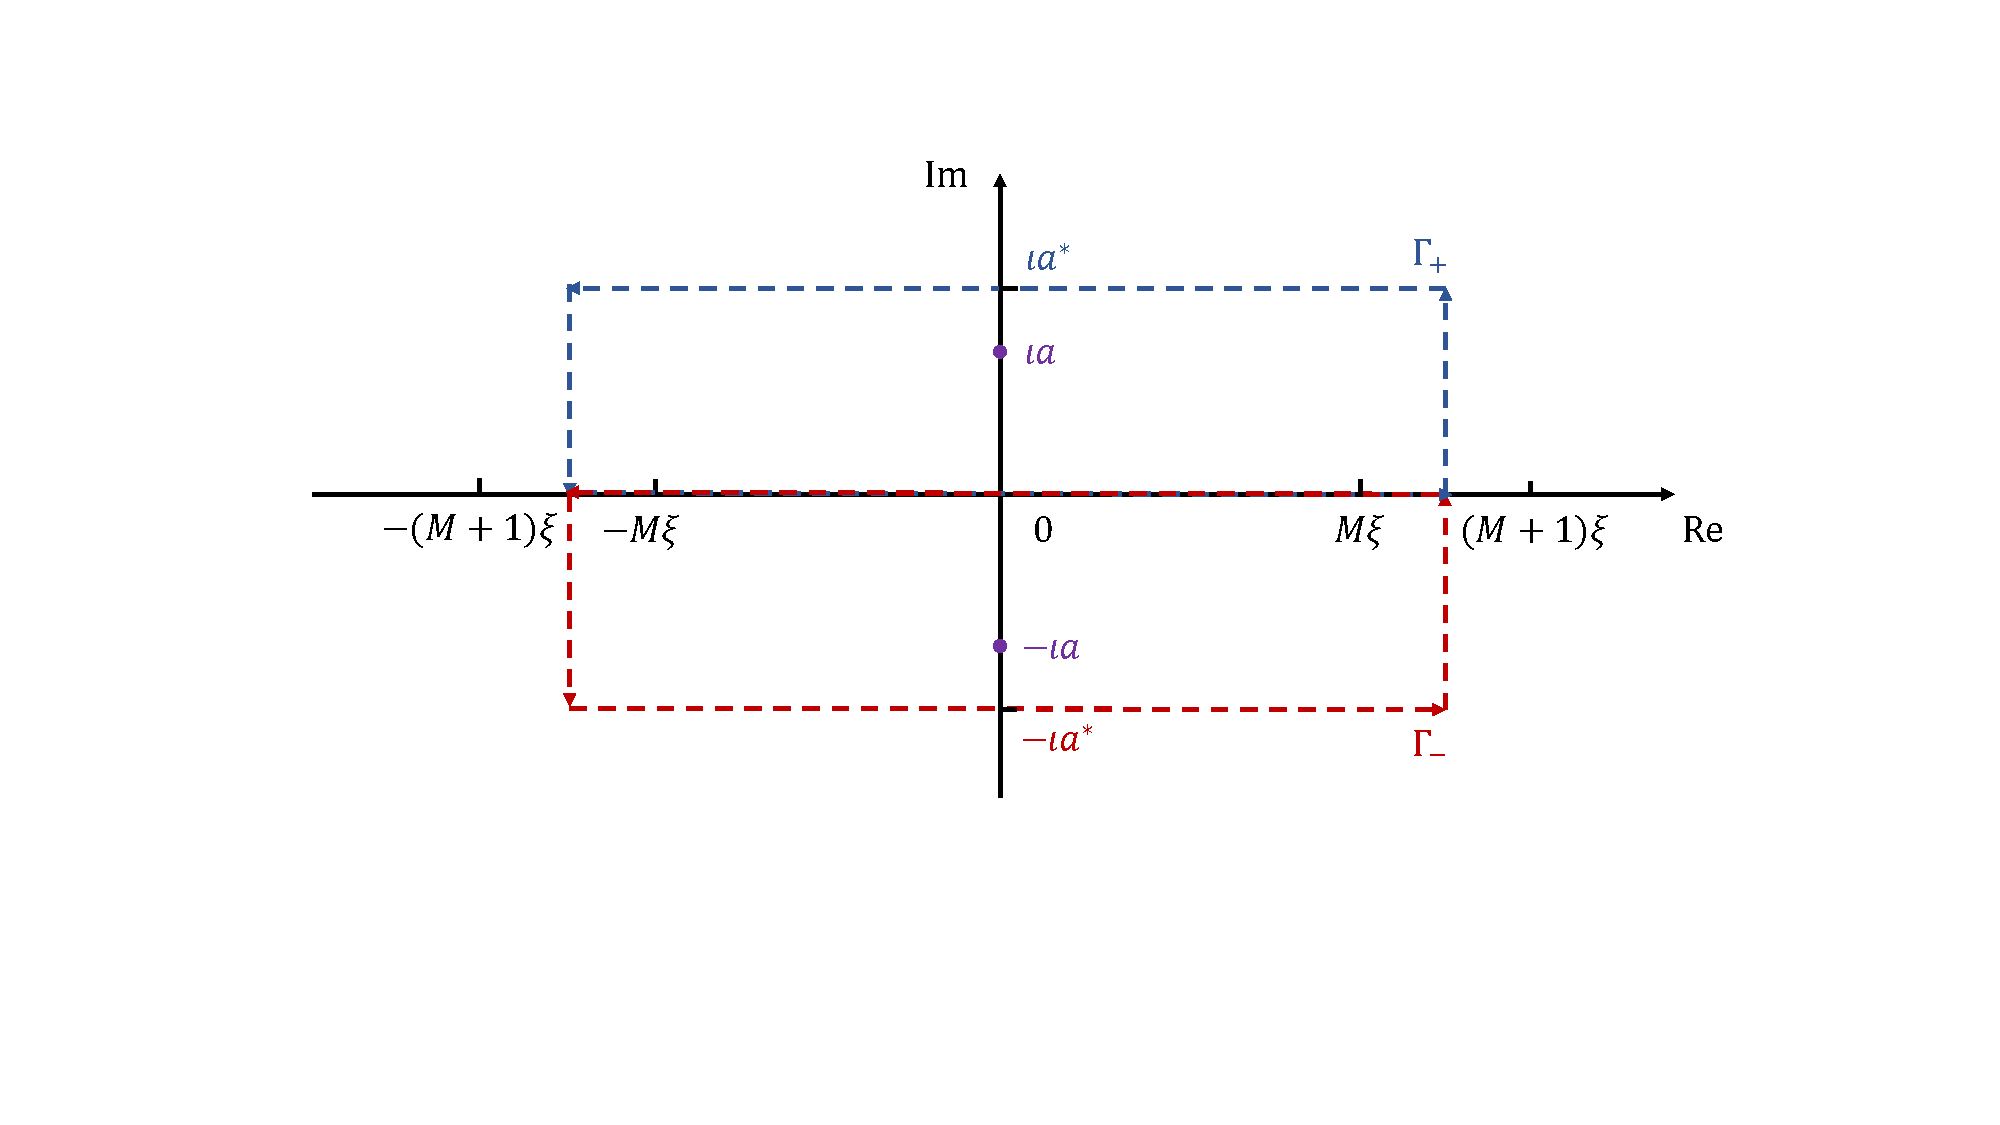
\includegraphics[width=0.8\textwidth]{figs/Trapezoidal.pdf}
    \caption{Integration contours in the error estimation of trapezoidal rule.}
    \label{fig:Trapezoidal}
    \end{center} 
\end{figure}

\section{The ideal-gas assumption}\label{app::ideal-gas}
Let $\bm{\mathcal{\psi}}$ represent a statistical quantity in an interacting particle system, and we aim to analyze its root mean square value given by
\begin{equation}\label{eq::deltaS}
    \delta \bm{\mathcal{\psi}}:=\sqrt{\frac{1}{N}\sum_{i=1}^{N}\|\bm{\mathcal{\psi}}_{i}\|^2},
\end{equation}
where $\bm{\mathcal{S}}_{i}$ denotes the quantity associated with particle $i$ (e.g., energy for one dimension or force for three dimensions). Assume that $\bm{\mathcal{\psi}}_{i}$ takes the form
\begin{equation}
	\bm{\mathcal{\psi}}_{i}=q_{i} \sum_{j \neq i} q_{j} \bm{\zeta}_{i j},
\end{equation}
due to the superposition principle of particle interactions, which implies that the total effect on particle $i$ can be expressed as the sum of contributions from each $i-j$ pair (including periodic images). Here, $\bm{\zeta}_{i j}$ represents the interaction between two particles. The ideal-gas assumption leads to the following relation
\begin{equation}
	\left\langle\boldsymbol{\zeta}_{i j} \boldsymbol{\zeta}_{i k}\right\rangle=\delta_{j k}\left\langle\boldsymbol{\zeta}_{i j}^2\right\rangle:=\delta_{j k} \zeta^2,
\end{equation}
where the expectation is taken over all particle configurations, and $\zeta$ is a constant. This assumption indicates that any two different particle pairs are uncorrelated, and the variance of each pair is expected to be uniform. In the context of computing the force variance of a charged system, this assumption implies that
\begin{equation}
	\left\langle\|\bm{\mathcal{\psi}}_{i}\|^2\right\rangle=q_{i}^2 \sum_{j, k \neq i} q_{j} q_k\left\langle\boldsymbol{\zeta}_{i j} \boldsymbol{\zeta}_{i k}\right\rangle \approx q_{i}^2 \zeta^2 Q,
\end{equation}
where $Q$ represents the total charge of the system. By applying the law of large numbers, one obtains $\delta\mathcal{\psi}\approx \zeta Q/\sqrt{N}$, which can be utilized for the mean-field estimation of the truncation error.

\section{The Debye-H$\ddot{\text{u}}$ckel approximation}\label{app::Debye}
Under the DH approximation, one is able to estimate functions associated with the $i$-th particle in the form:
\begin{equation}
	\mathscr{G}(\bm{r}_i)=\sum_{j\neq i}q_{j}e^{\m{i} \bm{k}\cdot\bm{\rho}_{ij}}f(z_{ij}),
\end{equation}
where $|f(z_{ij})|$ is bounded by a constant $C_f$ independent of $z_{ij}$. The DH theory considers the simplest model of an electrolyte solution confined to the simulation cell, where all $N$ ions are idealized as hard spheres of diameter $r_{a}$ carrying charge $\pm q$ at their centers. The charge neutrality condition requires that $N_+=N_-=N/2$. Let us fix one ion of charge $+q$ at the origin $r=0$ and consider the distribution of the other ions around it.

In the region $0<r\leq r_{a}$, the electrostatic potential $\phi(\bm{r})$ satisfies the Laplace equation $-\Delta\phi(\bm{r})=0$. For $r\geq r_{a}$, the charge density of each species is described by the Boltzmann distribution $\rho_{\pm}(\bm{r})=\pm qe^{\mp\beta q\phi(\bm{r})}\rho_r/2$ with number density $\rho_r=N/V$. In this region, the electrostatic potential satisfies the linearized Poisson-Boltzmann equation~\cite{levin2002electrostatic}:
\begin{equation}
	-\Delta \phi(\bm{r})=2\pi\left[q \rho_r e^{-\beta q\phi(\bm{r})}-q\rho_r e^{+\beta q\phi(\bm{r})}\right]\approx -4\pi \beta q^2\rho_r\phi(\bm{r}),
\end{equation}
and its solution is given by
\begin{equation}
	\phi(\bm{r})=\begin{cases}
		\dfrac{q}{4\pi r}-\dfrac{q\kappa}{4\pi (1+\kappa a)},& r<r_{a},\\[1em]
		\dfrac{qe^{\kappa a}e^{-\kappa r}}{4\pi r(1+\kappa a)},&r\geq r_{a},
	\end{cases}
\end{equation}
where $\kappa=\sqrt{\beta q^2\rho}$ denotes the inverse of Debye length $\lambda_{\text{D}}$. By this definition, the net charge density for $r>r_{a}$ is $\rho_>(\bm{r})=-\kappa^2\phi(\bm{r})$. Let us fix $\bm{r}_i$ at the origin. Given these considerations, for $r\geq r_a$, one obtains the following estimate:
\begin{equation}\label{eq::E.4}
	\begin{split}
		|\mathscr{G}(\bm{r}_i)|&\approx \left|\int_{\mathbb{R}^3\backslash B(\bm{r}_{i}, r_a)}\rho_>(\bm{r})e^{-\m{i} \bm{k}\cdot\bm{\rho}}f(z)d\bm{r}\right|\\
		&\leq \frac{q_iC_fe^{\kappa a}}{4\pi(1+\kappa a)}\int_{a}^{\infty}\frac{e^{-\kappa r}}{r}4\pi r^2dr\\
		&=q_iC_f\lambda_{\text{D}}^2.
	\end{split}
\end{equation}

It is remarked that upper bound Eq.~\eqref{eq::E.4} is derived under the continuum approximation. In the presence of surface charges, the charge distribution along the $z$-direction may lack spatial uniformity. However, due to the confinement of particle distribution between two parallel plates, the integral in Eq.~\eqref{eq::E.4} along the $z$-direction remains bounded. An upper bound in the form of $|\mathscr{G}(\bm{r}_i)|\leq C_s C_{f}q_i$ can still be expected, where $C_s$ is a constant related to the thermodynamic properties of the system.

\section{The Metropolis algorithm} \label{app::Metropolis}

In practice, the Metropolis algorithm~\cite{metropolis1953equation, hastings1970monte} is employed to generate a sequence $\{\bm{k}_{\eta}\}_{\eta=1}^{P}$ from $h(\bm{k})$. 
Since $\bm{k}\circ \bm{L}=2\pi \bm{m}$ with $\bm{m}$ an integer vector, one can conveniently sample from the discrete distribution $\mathcal{H}(\bm{m})=h(\bm{k})$ to equivalently generate $\bm{k}$. 
Once the current state of the Markov chain $\bm{m}_{\eta}=\bm{m}^{\text{old}}$ is known, the algorithm generates a random variable $\bm{m}^*$ with $m_{\xi}^*\sim \mathcal{N}[0,(\alpha L_{\xi})^2/2\pi^2]$, which is the normal distribution with mean zero and variance $(\alpha L_{\xi})^2/2\pi^2$. The new proposal is taken as $\bm{m}^{\text{new}}=\text{round}(m_{x}^*,m_{y}^*)$. To determine the acceptance rate, one obtains the proposal probability 
\begin{equation}
	q(\bm{m}^{\text{new}}|\bm{m}^{\text{old}})=\prod_{\xi\in\{x,y\}}q(m^{\text{new}}_{\xi}|m^{\text{old}}_{\xi})
\end{equation}
where
\begin{equation}
	\begin{split}
		q(m^{\text{new}}_{\xi}|m^{\text{old}}_{\xi})&=\sqrt{\frac{\pi}{(\alpha L_{\xi})^2}}\int_{m^{\text{new}}_{\xi}-\frac{1}{2}}^{m^{\text{new}}_{\xi}+\frac{1}{2}}e^{-\pi^2t^2/(\alpha L_{\xi})^2}dt\\[1em]
		&=\begin{cases}
			\erf\left(\dfrac{\pi}{2\alpha L_{\xi}}\right),&m_{\xi}^{\text{new}}=0,\\[1.15em]
			\dfrac{1}{2}\left[\erf\left(\dfrac{\pi(2|m_{\xi}^{\text{new}}|+1)}{2\alpha L_{\xi}}\right)-\erf\left(\dfrac{\pi(2|m_{\xi}^{\text{new}}|-1)}{2\alpha L_{\xi}}\right)\right],&m_{\xi}^{\text{new}}\neq 0.
		\end{cases}
	\end{split}
\end{equation}
It is worth noting that the proposal distribution $q(\bm{m}^{\text{new}}|\bm{m}^{\text{old}})$ in the Metropolis algorithm presented here does not depend on the current state $\bm{m}^{\text{old}}$. The Metropolis acceptance probability is computed using the formula:
\begin{equation}
	a(\bm{m}^{\text{new}}|\bm{m}^{\text{old}}):=\min\left\{\frac{\mathcal{H}(\bm{m}^{\text{new}})q(\bm{m}^{\text{old}}|\bm{m}^{\text{new}})}{\mathcal{H}(\bm{m}^{\text{old}})q(\bm{m}^{\text{new}}|\bm{m}^{\text{old}})},1\right\}.
\end{equation}
If the proposal is rejected, then $\bm{m}_{\eta+1}=\bm{m}_{\eta}$. If $\bm{m}^{\text{new}}$ is accepted, then $\bm{m}_{\eta+1}=\bm{m}^{\text{new}}$. The sampling procedure has a small error since $\mathcal{H}(\bm{m}^{\text{new}})\approx q(\bm{m}^{\text{new}}|\bm{m}^{\text{old}})$. Our numerical experiments show an average acceptance rate of over $90\%$. Additionally, one can set an integer downsampling rate $\mathscr{D}$, where only one sample is taken from every $\mathscr{D}$ samples, to reduce the correlation between batches in the Metropolis process.

\section{Physical quantities}\label{Sec::phyquan}

In this section, we will briefly describe how to calculate the physical quantities of interest in this paper.

To calculate the average concentration of the system along the $z$-direction, we first divide the interval $[0,H]$ into $250$ equally spaced bins. Then, every $100$ steps, we count the number of particles whose $z$-coordinate $r_z$ falls within each bin and calculate the ensemble average. After the simulation is completed, we divide the accumulated values by the length of each bin to obtain the average concentration. The MSD along $z$-direction, $\eta_{\text{msd},z}(t)$ at time $t$ is defined as
\begin{equation}
\eta_{\mathrm{msd},z}(t)=\left\langle\left|r_z\left(t+t_0\right)-r_z\left(t_0\right)\right|^2\right\rangle,
\end{equation}
with the bracket representing the ensemble average over $t_0$. The VACF along $z$-direction, $\eta_{\text{vacf},z}(t)$ at time $t$ is defined as
\begin{equation}
\eta_{\text {vacf},z}(t)=\left\langle v_z\left(t_0\right) v_z(t)\right\rangle,
\end{equation}
with the bracket representing the ensemble average over $t_0$. The total energy is defined as the sum of potential energy and kinetic energy. The potential energy is the sum of bond, angle, Coulomb, LJ and  {constraint} components, where the first two and the last one are not required for electrolyte solutions. 

Let $N$ is the number of particles, $\bm{r}_i=(r_{i,x},r_{i,y},r_{i,z})$, $\bm{v}_i=(v_{i,x},v_{i,y},v_{i,z})$ and $\bm{f}_i=(f_{i,x},f_{i,y},f_{i,z})$ represent the position, velocity and force of $i$th particle along each of three dimensions, respectively. The $z$-$z$ component subtracted from pressure tensor is computed by the formula
\begin{equation}
P_{zz}=\frac{1}{V} \sum_{i=1}^N\left(m_i v_{i,z} v_{i, z}+r_{i,z} f_{i,z}\right),
\end{equation}
where the two components in each term come from the kinetic energy and the virial contributions, respectively. It is remarked that the far-field component of  {the} virial associated with the Ewald decomposition requires the use of specialized methods~\cite{liang2022random}. 

% \chapter{Supplementary Results for Chapter 2}
% \label{chp_appendix_preliminaries}
% \section{Proof of Lemma~\ref{thm::SpectralExpansion}}\label{app::deriv}
By applying the Fourier transform to Poisson's equation
\begin{equation}\label{eq::B.1}
	-\Delta\phi_{\ell}(\bm{\rho},z)=4\pi g(\bm{\rho},z)\ast\tau(\bm{\rho},z),
\end{equation}
one obtains  
\begin{equation}\label{eq::B2}
	\widetilde{\phi}_{\ell}(\bm{h},\kappa)=\frac{4\pi}{h^2+\kappa^2}\widetilde{g}(\bm{h},\kappa)\widetilde{\tau}(\bm{h},\kappa)\quad\text{with}\quad \widetilde{g}(\bm{h},\kappa)=\sum_{j=1}^{N}q_{j} e^{-\m{i} \bm{h}\cdot\bm{\rho}_{j}}e^{-\m{i} \kappa z_{j}}
\end{equation}
via the convolution theorem and the Poisson summation formula (see Lemmas~\ref{lem::Convolution} and \ref{lem::Poisson}, respectively). Applying the inverse Fourier transform to Eq.~\eqref{eq::B2} yields
\begin{equation}\label{eq::phil}
	\phi_{\ell}(\bm{\rho},z)=\frac{2}{L_xL_y}\sum_{j=1}^{N}q_{j}\sum_{\bm{h}\neq\bm{0}}\int_{\mathbb{R}}\frac{e^{-(h^2+\kappa^2)/(4\alpha^2)}}{h^2+\kappa^2}e^{-\m{i} \bm{h}\cdot(\bm{\rho}-\bm{\rho}_{j})}e^{-\m{i} \kappa(z-z_{j})}d\kappa + \phi^{\bm{0}}_{\ell}(z),
\end{equation}
where $\phi^{\bm{0}}_{\ell}(z)$ is the contribution from zero mode. From \cite{oberhettinger2012tables}, one has 
\begin{equation}\label{eq::integral}
	\int_{\mathbb{R}} \frac{e^{-(h^2+\kappa^2)/(4\alpha^2)}}{h^2+\kappa^2} e^{-\m{i} \kappa z} d\kappa = \frac{\pi}{2h} \left[\xi^{+}(h,z)+\xi^{-}(h,z)\right]
\end{equation}
for $\bm{h}\neq\bm{0}$, where $\xi^{\pm}(h,z)$ are defined via Eq.~\eqref{eq::xi20}. Substituting Eq.~\eqref{eq::integral} into the first term of Eq.~\eqref{eq::phil} yields $\phi_{\ell}^{\bm{h}}(\bm{r})$ defined via Eq.~\eqref{eq:philk}.

By Theorem~\ref{order}, the zero-frequency term $\phi^{\bm{0}}_{\ell}(z)$ always exists and its derivation is very subtle. Let us apply the 2D Fourier transform (see Lemma~\ref{lem::2dfourier}) to Poisson's equation Eq.~\eqref{eq::B.1} only on periodic dimensions, and then obtain
\begin{equation}\label{eq::B.5}
	(-\partial_z^2+h^2)\widehat{\phi}_{\ell}(\bm{h},z)=4\pi\widehat{g}(\bm{h},z)\ast_{z}\widehat{\tau}(\bm{h},z),
\end{equation}
where $\ast_z$ indicates the convolution operator along $z$ dimension. Simple calculations suggest
\begin{equation}
	\widehat{g}(\bm{h},z)=\sum_{j=1}^{N}q_{j} e^{-\m{i} \bm{h}\cdot\bm{\rho}_{j}}\delta(z-z_{j}),\quad\text{and}\quad \widehat{\tau}(\bm{h},z)=\frac{\alpha}{\sqrt{\pi}} e^{-h^2/(4\alpha^2)}e^{-\alpha^2z^2}.
\end{equation}
The solution of Eq.~\eqref{eq::B.5} for $\bm{k}=\bm{0}$ can be written as the form of double integral that is only correct up to a linear mode,
\begin{equation}\begin{split}
		\phi_{\ell}^{\bm{0}}(z)&=-\frac{4\pi}{L_xL_y}\int_{-\infty}^{z}\int_{-\infty}^{z_1}\widehat{g}(\bm{0},z_2)\ast_{z_2}\widehat{\tau}(\bm{0},z_2)dz_2dz_1+A_0z+B_0\\
		&=-\frac{2\pi}{L_xL_y}\sum_{j=1}^{N}q_{j}\left[z-z_{j}+(z-z_{j})\erf\left(\alpha(z-z_{j})\right)+\frac{e^{-\alpha^2(z-z_{j})^2}}{\sqrt{\pi}\alpha}\right]+A_0z+B_0.
	\end{split}
\end{equation}
To analyze the short-range component $\phi_{s}(\bm{\rho},z)$ using a procedure similar to Eqs.~\eqref{eq::B.1}-\eqref{eq::integral}, one obtains
\begin{equation}\begin{split}
		\phi_{s}^{\bm{0}}(z) =& \frac{\pi}{L_x L_y} \sum_{j=1}^{N} \lim_{\bm{h}\rightarrow\bm{0}} \frac{1}{h} \left[2e^{-h|z|}-\xi^{+}(\bm{h},z) - \xi^{-}(\bm{h},z)\right]\\
		=& \frac{2\pi}{L_xL_y}\sum_{j=1}^{N}q_{j}\left[-|z-z_{j}|+(z-z_{j})\erf\left(\alpha(z-z_{j})\right)+\frac{e^{-\alpha^2(z-z_{j})^2}}{\sqrt{\pi}\alpha}\right].
	\end{split}
\end{equation}
Since $\phi_{s}^{\bm{0}}(z)+\phi_{\ell}^{\bm{0}}(z)$ matches the boundary condition Eq.~\eqref{eq::boundary1} as $z\rightarrow \pm\infty$ and by the charge neutrality condition, one solves 
\begin{equation}
	A_0 = \frac{2\pi}{L_xL_y}\sum_{j=1}^{N}q_{j}z \equiv 0,\quad \text{and}\quad B_0=-\frac{2\pi}{L_xL_y}\sum_{j=1}^{N}q_{j}z_{j}.
\end{equation}
This result finally gives 
\begin{equation}
	\phi_{\ell}^{\bm{0}}(z)=-\frac{2\pi}{L_xL_y}\sum_{j=1}^{N}q_{j}\left[(z-z_{j})\erf\left(\alpha(z-z_{j})\right)+\frac{e^{-\alpha^2(z-z_{j})^2}}{\sqrt{\pi}\alpha}\right].
\end{equation}

%and can be written as 
%\begin{equation}\phi^{\bm{0}}_{\ell}(\bm{\rho},z)=\frac{\pi}{L_x L_y}\sum_{j=1}^{N}q_{j}\lim_{\bm{k}\rightarrow \bm{0}}\frac{e^{\m{i} \bm{k}\cdot(\bm{\rho}-\bm{\rho}_{j})}}{k}\left[\xi^{+}(k,z)+\xi^{-}(k,z)\right].\end{equation} By Taylor expansion with respect to $\bm{k}$, one gets \begin{equation}\begin{split}\phi^{\bm{0}}_{\ell}(\bm{\rho},z)=&\frac{\pi}{L_x L_y}\sum_{j=1}^{N}q_{j}\lim_{\bm{k}\rightarrow \bm{0}}\frac{1+\m{i} \bm{k}\cdot(\bm{\rho}-\bm{\rho}_{j})+O(k^2)}{k}\Bigg[2-2k(z-z_{j})\erf(\alpha (z-z_{j}))\\&-\frac{2ke^{-\alpha^2(z-z_{j})^2}}{\sqrt{\pi}\alpha}+O(k^2)\Bigg]\\=&-\frac{2\pi}{L_xL_y}\sum_{j=1}^{N}q_{j}\left[(z-z_{j})\erf(\alpha (z-z_{j})-\frac{e^{-\alpha^2(z-z_{j})^2}}{\sqrt{\pi}\alpha}\right]\end{split}\end{equation}

% \section{Systems with charged slabs}\label{sec::sysslabs}
% In the presence of charged slabs, boundary layers naturally arise -- opposite ions accumulate near the interface, forming an electric double layer. The structure of electric double layers plays essential role for properties of interfaces and has caught much attention~\cite{messina2004effect,breitsprecher2014coarse,moreira2002simulations}. Since charges on the slabs are often represented as a continuous surface charge density, we present the Ewald2D formulation with such a situation can be well treated.

% Without loss of generality, one assumes that the two charged slab walls are located at $z=0$ and $z=L_z$ and with smooth surface charge densities $\sigma_{\mathrm{bot}}(\bm{\rho})$ and $\sigma_{\mathrm{top}}(\bm{\rho})$, respectively. Note that both $\sigma_{\mathrm{bot}}(\bm{\rho})$ and $\sigma_{\mathrm{top}}(\bm{\rho})$ are doubly-periodic according to the quasi-2D geometry. 
% Under such setups, the potential $\phi$ can be written as the sum of particle-particle and particle-slab contributions,
% \begin{align}
% 	\phi(\bm{r})=\phi_{\text{p-p}}(\bm{r})+\phi_{\text{p-s}}(\bm{r}).
% \end{align}
% Here, $\phi_{\text{p-p}}$ satisfies Eq.~\eqref{eq::Poisson} associated with the boundary condition Eq.~\eqref{eq::boundary2}. Note that Eq.~\eqref{eq::boundary1} does not apply since the particles are overall non-neutral. $\phi_{\text{p-s}}$ satisfies 
% \begin{equation}\label{eq::PoionWall}
% 	-\Delta \phi_{\text{p-s}}(\bm{r}) = 4\pi h(\bm{r}), \quad \text{with}~ h(\bm{r}) =  \sigma_{\mathrm{bot}}(\bm{\rho}) \delta(z) + \sigma_{\mathrm{top}}(\bm{\rho}) \delta(z-L_z),
% \end{equation}
% with the boundary condition
% \begin{equation}\label{eq::boundionwall}
% 	\lim_{z\rightarrow\pm\infty}\phi_{\text{p-s}}(\bm{r})=\mp \frac{2\pi}{L_xL_y}\left(\int_{\mathcal{R}^2}\sigma_{\mathrm{bot}}(\bm{\rho})|z|d\bm{\rho}+\int_{\mathcal{R}^2}\sigma_{\mathrm{top}}(\bm{\rho})|z-L_z|d\bm{\rho}\right)
% \end{equation}
% which is simply the continuous analog of Eq.~\eqref{eq::boundary2}. 

% % The charge neutrality condition of the system reads
% % \begin{equation}\label{eq::chargeneu}
% 	% \sum_{i=1}^{N}q_{i}+\int_{\mathcal{R}^2}\left[\sigma_{\mathrm{top}}(\bm{\rho})+\sigma_{\mathrm{bot}}(\bm{\rho})\right]d\bm{\rho}=0,
% 	% \end{equation}
% % which leads to the well-definedness of potential $\phi$ together with the DPBCs imposed. 
% The potential $\phi_{\text{p-p}}$ then follows immediately from Lemma~\ref{thm::SpectralExpansion}
% \begin{equation}\label{eq::phiion-ion}
% 	\phi_{\text{p-p}}(\bm{r}_{i})=\phi_{s}(\bm{r}_{i}) + \sum_{\bm{k}\neq\bm{0}} \phi_{\ell}^{\V{k}}(\bm{r}_{i}) + \phi_{\ell}^{\V{0}}(\bm{r}_{i}) - \phi_{\text{self}}^{i},
% \end{equation}
% with each components given by Eqs.~\eqref{eq:phi_s}, \eqref{eq:philk}, \eqref{eq:phil0}, and \eqref{eq::self}, respectively. 
% The 2D Fourier series expansion of~$\phi_{\text{p-s}}$ is provided in the following Theorem~\ref{thm::ionwall}, where its convergence rate is controlled by the smoothness of surface charge densities.
% \begin{thm}\label{thm::ionwall}
% 	Suppose that $\widehat{\sigma}_{\mathrm{bot}}$ and $\widehat{\sigma}_{\mathrm{top}}$ are two-dimensional Fourier transform (see Lemma~\ref{lem::2dfourier}) of $\sigma_{\mathrm{bot}}$ and $\sigma_{\mathrm{top}}$, respectively. By Fourier analysis, the particle-slab component of the electric potential is given by
% 	\begin{equation}\label{eq::phiionwall}
% 		\phi_{\emph{p-s}}(\bm{r}_{i}) = \frac{2\pi}{L_xL_y}\sum_{\bm{k}\neq \bm{0}}\frac{e^{\m{i} \bm{k}\cdot\bm{\rho}_{i}}}{k}\left[\widehat{\sigma}_{\mathrm{bot}}(\bm{k})e^{-k|z_{i}|}+\widehat{\sigma}_{\mathrm{top}}(\bm{k})e^{-k|z_{i}-L_z|}\right]+\phi_{\emph{p-s}}^{\bm{0}}(\bm{r}_{i})\;,
% 	\end{equation}
% 	where the 0-th mode reads
% 	\begin{equation}\label{eq::phionwallzero}
% 		\phi_{\emph{p-s}}^{\bm{0}}(\bm{r}_{i})=-\frac{2\pi}{L_xL_y}\Big[\widehat{\sigma}_{\mathrm{bot}}(\bm{0})|z_{i}|+\widehat{\sigma}_{\mathrm{top}}(\bm{0})|z_{i}-L_z|\Big]\;.
% 	\end{equation}
% \end{thm}
% \begin{proof}
% 	For $\bm{k}\neq\bm{0}$, applying the quasi-2D Fourier transform to both sides of Eq.~\eqref{eq::PoionWall} yields
% 	\begin{equation}
% 		\widetilde{\phi}_{\text{p-s}}(\bm{k},\kappa)=\frac{4\pi}{k^2+\kappa^2}\left[\widehat{\sigma}_{\mathrm{bot}}(\bm{k})+\widehat{\sigma}_{\mathrm{top}}(\bm{k})e^{-\m{i} \kappa L_z}\right]\;.
% 	\end{equation}
% 	For $\bm{k}=0$, one first applys the 2D Fourier transform in $xy$ to obtain
% 	\begin{equation}
% 		\left(-\partial_z^2+k^2\right)\widehat{\phi}(\bm{k},z)=4\pi\left[\widehat{\sigma}_{\mathrm{bot}}(\bm{k})\delta(z)+\widehat{\sigma}_{\mathrm{top}}(\bm{k})\delta(z-L_z)\right]\;.
% 	\end{equation}
% 	By integrating both sides twice and taking $\bm{k}=0$, the $0$-th mode follows 
% 	\begin{equation}
% 		\widehat{\phi}(\bm{0},z)=-2\pi\left[\widehat{\sigma}_{\mathrm{bot}}(\bm{0})|z|+\widehat{\sigma}_{\mathrm{top}}(\bm{0})|z-L_z|\right]+A_0z+B_0\;,
% 	\end{equation}
% 	where $A_0$ and $B_0$ are undetermined constants. 
% 	Finally, applying the corresponding inverse transforms to $\widetilde{\phi}_{\text{p-s}}(\bm{k},\kappa)$ and $\widehat{\phi}(\bm{0},z)$ such that the boundary conditions Eq.~\eqref{eq::boundionwall} is matched, one has $A_0=B_0=0$. The proof of Eqs.~\eqref{eq::phiionwall}-\eqref{eq::phionwallzero} is then completed. 
% \end{proof}


% Consider the ideal case that both $\sigma_{\mathrm{bot}}$ and $\sigma_{\mathrm{top}}$ are uniformly distributed. This simple setup is widely used in many studies on interface properties. Since in this case all nonzero modes vanish, one has
% \begin{equation}\label{eq:spectial}
% 	\phi_{\text{p-s}}(\bm{r}_{i})=\phi_{\text{p-s}}^{\bm{0}}(\bm{r}_{i})=-2\pi\left[\sigma_{\mathrm{top}}(L_z - z_{i})+\sigma_{\mathrm{bot}}(z_{i} - 0))\right]\;,
% \end{equation}
% for all $z_{i}\in [0, L_z]$. 
% Here zero is retained to indicate the location of bottom slab. 

% For completeness, Proposition \ref{welldefinedness} provides the result of the well-definedness.
% \begin{prop} \label{welldefinedness}
% 	The total electrostatic potential $\phi$ is well-defined. 
% \end{prop}
% \begin{proof}
% 	For any finite $z$, $\phi$ is clearly well defined. Consider the case of $z\rightarrow \pm \infty$.
% 	By boundary conditions ~\eqref{eq::boundary2} and \eqref{eq::boundionwall} and the charge neutrality condition Eq.~\eqref{eq::chargeneu}, one has
% 	\begin{equation}
% 		\begin{split}
% 			\lim_{z\rightarrow \pm \infty}\phi(\bm{r})&=\lim_{z\rightarrow \pm \infty}\left[\phi_{\text{p-p}}(\bm{r})+\phi_{\text{p-s}}(\bm{r})\right]\\
% 			&=\pm\frac{2\pi}{L_xL_y}\left[\sum_{j=1}^{N}q_{j}z_{j}+\int_{\mathcal{R}^2}\left(0\sigma_{\mathrm{bot}}(\bm{\rho})+L_z\sigma_{\mathrm{top}}(\bm{\rho})\right)d\bm{\rho}\right]
% 		\end{split}
% 	\end{equation}
% 	which is a finite constant. Thus the proof is completed.
% \end{proof}

% For the the particle-slab interaction formulation, we observe a constant discrepancy between Eq.~\eqref{eq:spectial} derived here and those in literature~\cite{dos2017simulations,yi2017note}. 
% It is because here one starts with the precise Ewald2D summation approach, different from the approach of employing approximation techniques to transform the original doubly-periodic problem into a triply-periodic problem first, and subsequently introducing charged surfaces. 
% This constant discrepancy makes no difference in force calculations for canonical ensembles. 
% However, for simulations under isothermal-isobaric ensembles, this $L_z$-dependent value is important for the pressure calculations~\cite{li2024noteaccuratepressurecalculations}. 
% And one should use Eq.~\eqref{eq:spectial} derived here for correct simulations.

% Based on the expression of electrostatic potential $\phi$ derived above, the total electrostatic energy can be computed via the Ewald2D summation formula:  
% \begin{align}\label{eq::34}
% 	U = U_{\text{p-p}} + U_{\text{p-s}}, \quad \text{with} \quad U_{\text{p-p}} := U_{s} + \sum_{\bm{k}\neq\bm{0}}U_{\ell}^{\bm{k}}+U_{\ell}^{\bm{0}}- U_{\text{self}}\;,
% \end{align}
% where $U_*=\sum_{i}\phi_*$ with $*$ representing any of the subscripts used in Eq.~\eqref{eq::34}.

\section{Proof of Theorem~\ref{thm:ewald2d_phi_error}}\label{app:phierr}
We begin by considering the real space truncation error of electrostatic potential 
\begin{equation}
	\mathscr{E}_{\phi_{s}}(r_c,\alpha)(\bm{r}_{i}) = \sum_{|\bm{r}_{ij} + \V{\mathcal{M}}|>r_c}q_{j} \frac{\erfc(\alpha|\bm{r}_{ij} + \V{\mathcal{M}}|)}{|\bm{r}_{ij} + \V{\mathcal{M}}|}
\end{equation}
for $i$th particle, which involves neglecting interactions beyond $r_c$. By the analysis in \ref{app::ideal-gas}, this part of error can be approximated by $\delta\mathscr{E}_{\phi_{s}}$ with 
\begin{equation}\label{eq::delta^2phi}
	\delta^2\mathscr{E}_{\phi_{s}}=  \frac{1}{V}\sum_{j=1}^{N}q_{j}^2\int_{r_c}^{\infty}\frac{\erfc(\alpha r)^2}{r^2}4\pi r^2dr=\frac{4\pi Q}{V}\mathscr{Q}_{\emph{s}}(\alpha,r_c),
\end{equation}
where $\mathscr{Q}_{\emph{s}}(\alpha,r_c)$ is defined via Eq.~\eqref{eq::Qs2}. Note that the $\erfc(r)$ function satisfies (\cite{olver1997asymptotics}, pp. 109-112)
\begin{equation}\label{eq::asyerfc}
	\erfc(r)=\frac{e^{-r^2}}{\sqrt{\pi}}\sum_{m=0}^{\infty}(-1)^{m}\left(\frac{1}{2}\right)_mz^{-(2m+1)}
\end{equation}
as $r\rightarrow \infty$, where $(x)_m=x(x-1)\cdots(x-m+1)=x!/(x-m)!$ denotes the Pochhammer's symbol. Substituting Eq.~\eqref{eq::asyerfc} into Eq.~\eqref{eq::delta^2phi} and truncating at $m=1$ yields Eq.~\eqref{eq::Qs}. 

The Fourier space error, by~\ref{app::deriv}, is given by
\begin{equation}
	\mathscr{E}_{\phi_{\ell}}(k_c,\alpha)(\bm{r}_{i})=\frac{2}{L_xL_y}\sum_{j=1}^{N}q_{j}\sum_{|\bm{h}|>k_c}\int_{\mathbb{R}}\frac{e^{-(h^2+\kappa^2)/(4\alpha^2)}}{h^2+\kappa^2}e^{-\m{i} \bm{h}\cdot(\bm{\rho}-\bm{\rho}_{j})}e^{-\m{i} \kappa(z-z_{j})}d\kappa.
\end{equation}
For a large $k_c$, one can safely replace the truncation condition with $|\bm{h}+\kappa|>k_c$, resulting in
\begin{equation}
	\begin{split}
		\mathscr{E}_{\phi_{\ell}}(k_c,\alpha)(\bm{r}_{i})&\approx \frac{1}{2\pi^2}\sum_{j=1}^{N}q_{j} \int_{k_c}^{\infty}\int_{-1}^{1}\int_{0}^{2\pi}e^{-h^2/(4\alpha^2)}e^{-i h r_{ij}\cos\varphi}d\theta d\cos\varphi dh\\
		&=\frac{2}{\pi}\int_{k_c}^{\infty}\sum_{j=1}^{N}q_{j}\frac{\sin(h r_{ij})}{h r_{ij}}e^{-h^2/(4\alpha^2)}dh.
	\end{split}
\end{equation}
Here, the summation over Fourier modes is approximated using an integral similar to Eq.~\eqref{eq::integral2}, and one chooses a specific $(h,\theta,\varphi)$ so that the coordinate along $\cos\theta$ of $\bm{h}$ is in the direction of a specific vector $\bm{r}$, and $\bm{h}\cdot\bm{r}=h r \cos\varphi$.
The resulting formula is identical to Eq.~(21) in \cite{kolafa1992cutoff} for the fully-periodic case, and $\delta \mathscr{E}_{\phi_{\ell}}$ can be derived following the approach in \cite{kolafa1992cutoff}. 

\chapter{Supplementary Results for Error Estimations}
\label{chp_appendix_icm}
\section{Numerical validations for error estimations in energy}\label{sec:numeric_energy}

In this section, we present supplementary results for the numerical validations for error estimations in electrostatic energy, complementing the main text. Figures~\ref{fig:icm_error} to~\ref{fig:error_icm_pad_gamma_1} correspond one-to-one with Figures 1 to 4 in the main text, maintaining the same systems and parameter settings as those used in the force calculation results. The dashed lines in these figures represent the fitted curves based on our theoretical estimation given in Eq.~(52) of the main text. The energy error results exhibit similar trends to the force errors and align well with our theoretical predictions.


\begin{figure}[htbp]
    \centering
    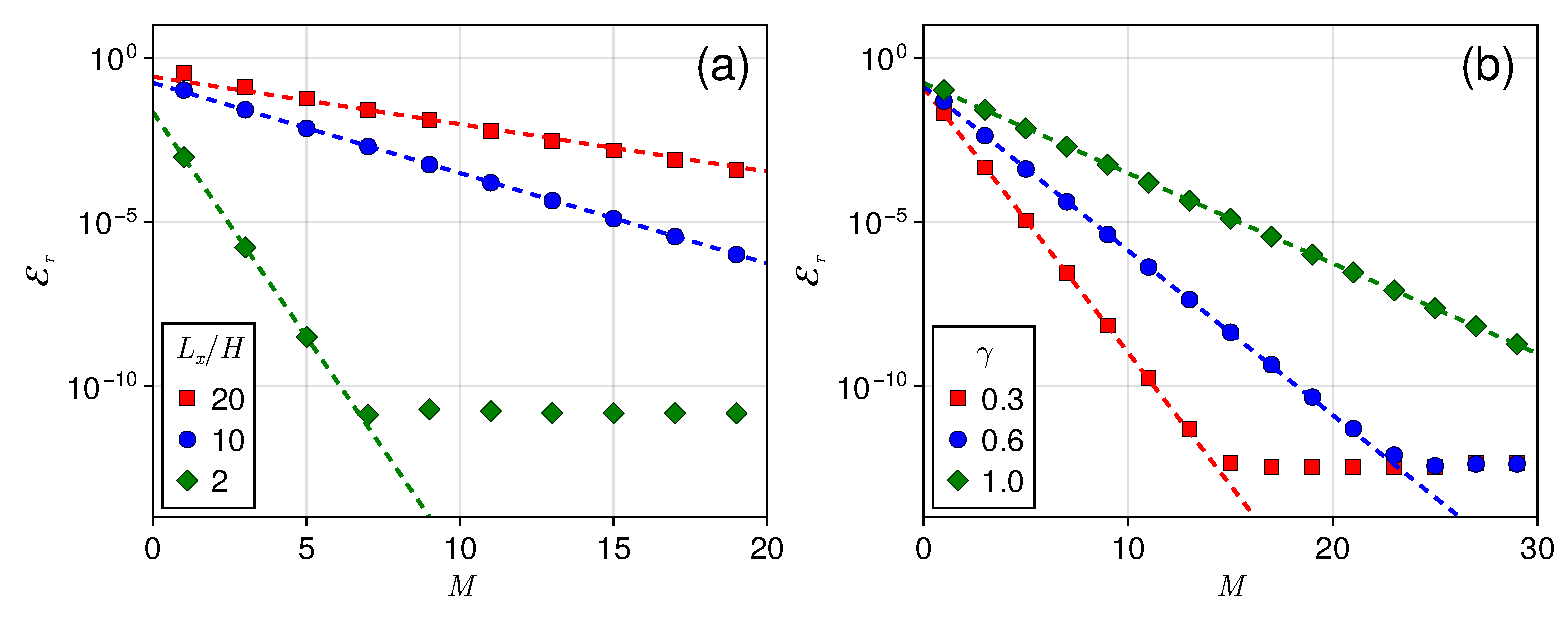
\includegraphics[width=0.98\linewidth]{figs/icm_error.pdf}
    \caption{
        Relative errors of energy due to truncation of image charges are presented. The dashed lines represent the fitted decay rate, as described in Eq. (54) in the main text. In panel (a) we set $\gamma_{\T u} = \gamma_{\T d} = 1$ and consider system heights of $H = 0.5, 1$ and $5$. In panel (b), we set $H = 1$ while varying $\gamma_{\T u} = \gamma_{\T d} = \gamma = 0.3, 0.6$ and $1$. 
        %The scope of the fitted lines are fixed to be $\lg(\gamma e^{-2\pi H / L_x})$, which is the theoretical value.
    }
    \label{fig:icm_error}
\end{figure}


\begin{figure}[htbp]
    \centering
    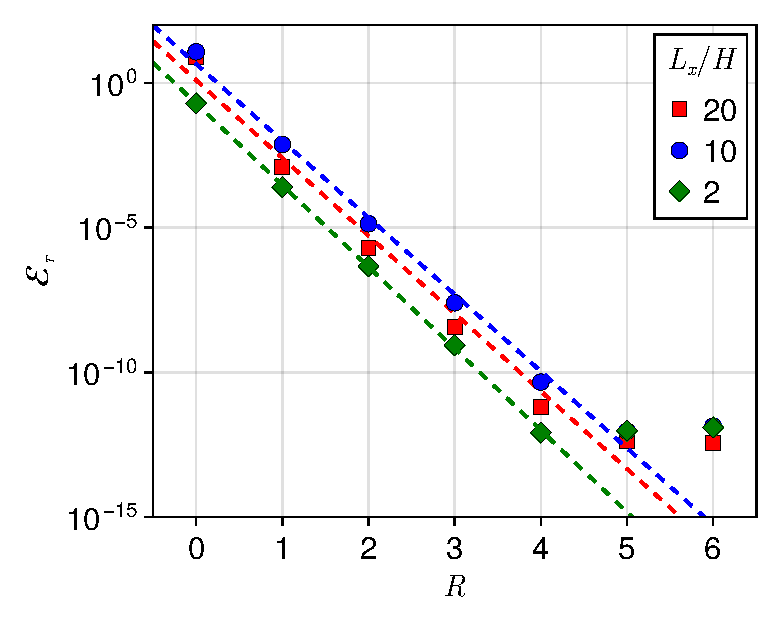
\includegraphics[width=0.49\linewidth]{figs/elc_error.pdf}
    \caption{Relative error of energy of reformulating the Ewald2D summation as 3D ones are presented. We set $\gamma_{\T u} = \gamma_{\T d} = 0$ and consider system heights of $H = 0.5, 1, 5$. Here $P = (L_z - H) / L_x$ denotes the padding ratio.}
    \label{fig:elc_error}
\end{figure}

\begin{figure}[htbp]
    \centering
    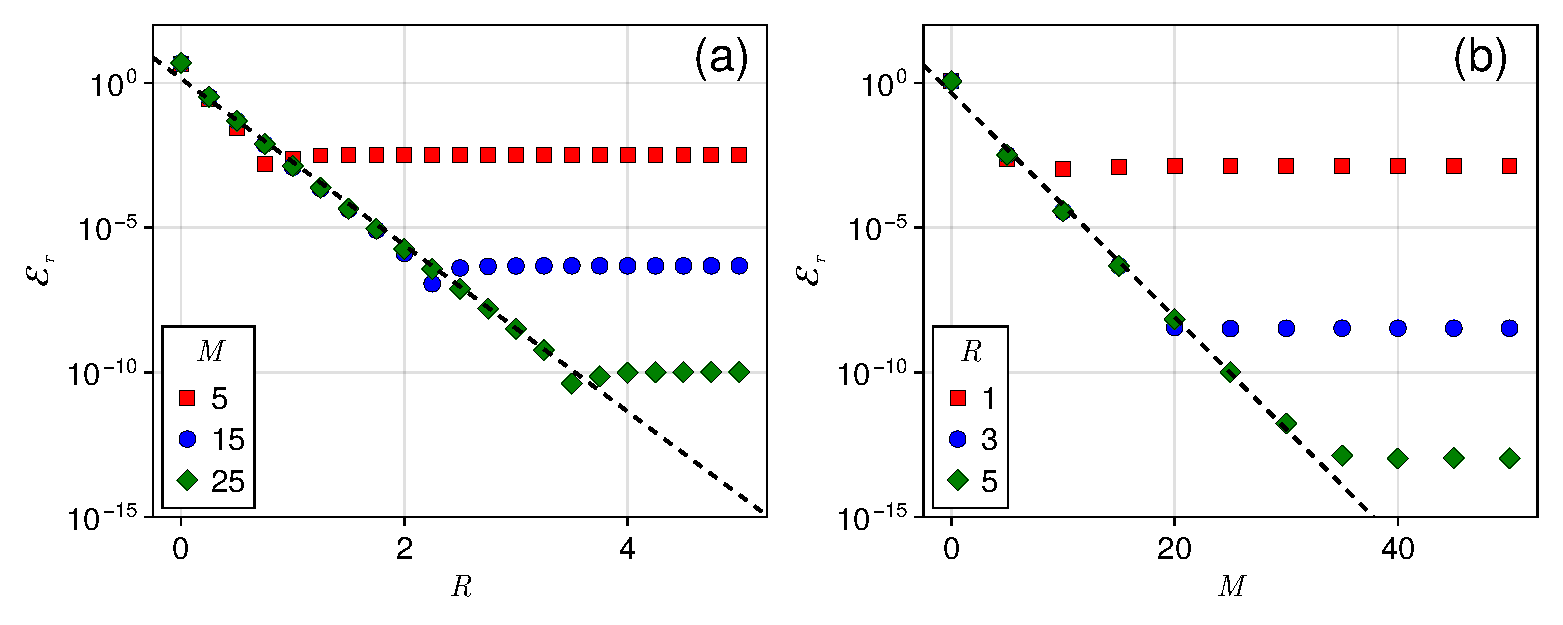
\includegraphics[width=0.98\linewidth]{figs/error_icm_pad_gamma_0.6.pdf}
    \caption{Relative error of energy in dielectric-confined Coulomb system with parameters $\gamma_{\T u} = \gamma_{\T d} = \gamma = 0.6$ and $H = 0.5$. Panel (a) illustrates error evolution with fixed image charge layers ($M = 5,~15,~25$) under varying padding ratios ($P$), whereas panel (b) demonstrates error progression with fixed $P = 1,~3,~5$ across increasing $M$.}
    \label{fig:error_icm_pad_gamma_0.6}
\end{figure}

\begin{figure}[htbp]
    \centering
    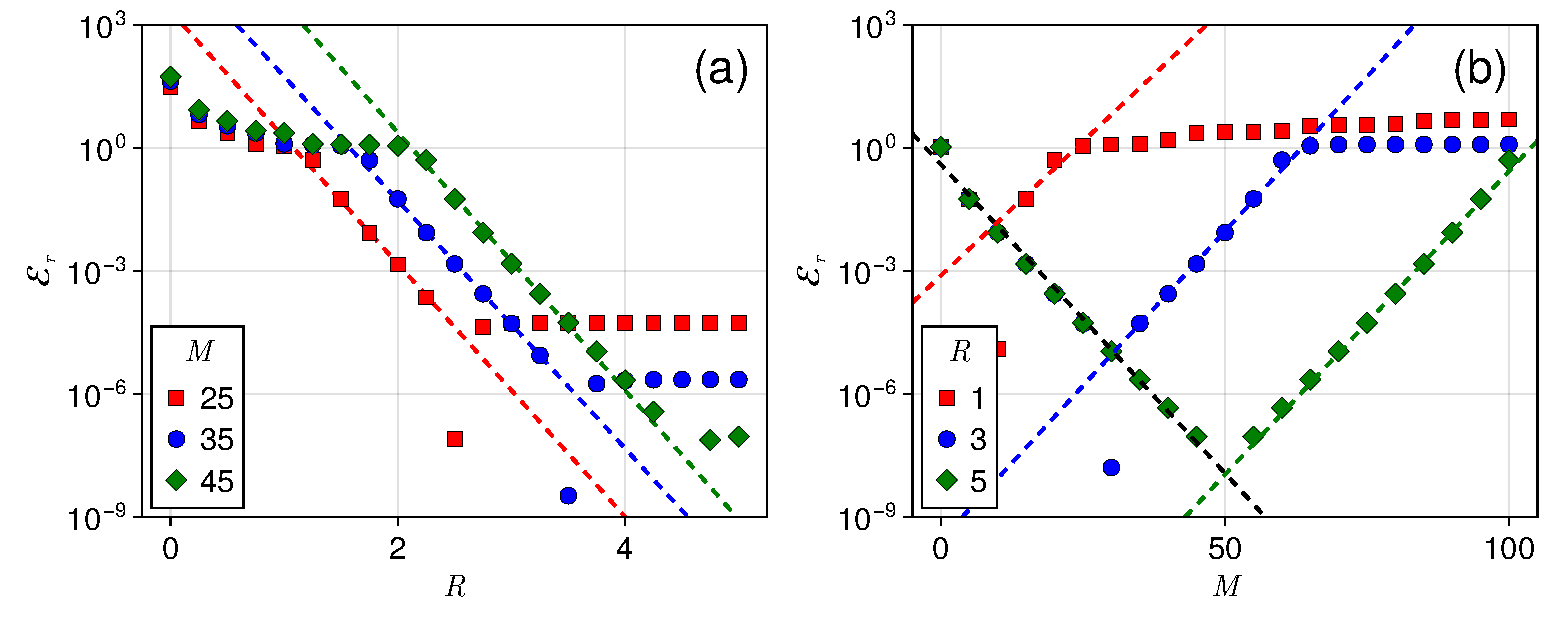
\includegraphics[width=0.98\linewidth]{figs/error_icm_pad_gamma_1.pdf}
    \caption{Relative error of energy in dielectric-confined Coulomb system with parameters $\gamma_{\T u} = \gamma_{\T d} = \gamma = 1$ and $H = 0.5$. Panel (a) illustrates error evolution with fixed image charge layers ($M = 5,~15,~25$) under varying padding ratios ($P$), whereas panel (b) demonstrates error progression with fixed $P = 1,~3,~5$ across increasing $M$.}
    \label{fig:error_icm_pad_gamma_1}
\end{figure}

\section{Challenge associated with strongly-confined systems}
In practical simulations, such as when studying thin membranes, ion transport in slit channels and supercapacitors, accurately capturing the effects of nanoconfinement, i.e., when $L_{x,y} / H\gg 1$, is crucial.
Previous numerical studies have found that more image layers are needed to achieve satisfactory accuracy for confined systems~\cite{dos2015electrolytes}. 
To further investigate the numerical properties of strongly-confined systems, we present the errors in force in Fig.~\ref{fig:icm_elc_error_force}, where we fix $L_x=L_y=10$, $R=(L_z-H)/L_x = 5$ and consider system heights $H = 0.5, 1, 5$ while varying the number of image charge layers $M$. 
In Fig.~\ref{fig:icm_elc_error_force} (a), for $\gamma = 0.6$, we observe that the error decays exponentially as $M$ increases for $H = 0.5$ and $H = 1$. 
However, for $H = 5$, where $|g_{\T u}g_{\T d}|>1$, the error becomes non-monotonic as $M$ increases, 
which is consistent with our theoretical predictions as discussed in the main text.
In Fig.~\ref{fig:icm_elc_error_force} (b), with $\gamma = 1$, we observe a similar non-monotonic pattern for all aspect ratios. 
It is important to note that, the rate of error decrease/increase depends on the aspect ratio $L_x/H$. 
A higher aspect ratio leads to a slower increase or decrease in errors, as $M$ is less or greater than the critical value that minimizes the error, respectively. 
This also highlights the computational challenge associated with strongly-confined systems -- to achieve the same accuracy, a much larger $M$ is required compared to non-confined systems.
Same conclusions hold for the errors in energy, as shown in Fig.~\ref{fig:icm_elc_error}.

\begin{figure}[htbp]
    \centering
    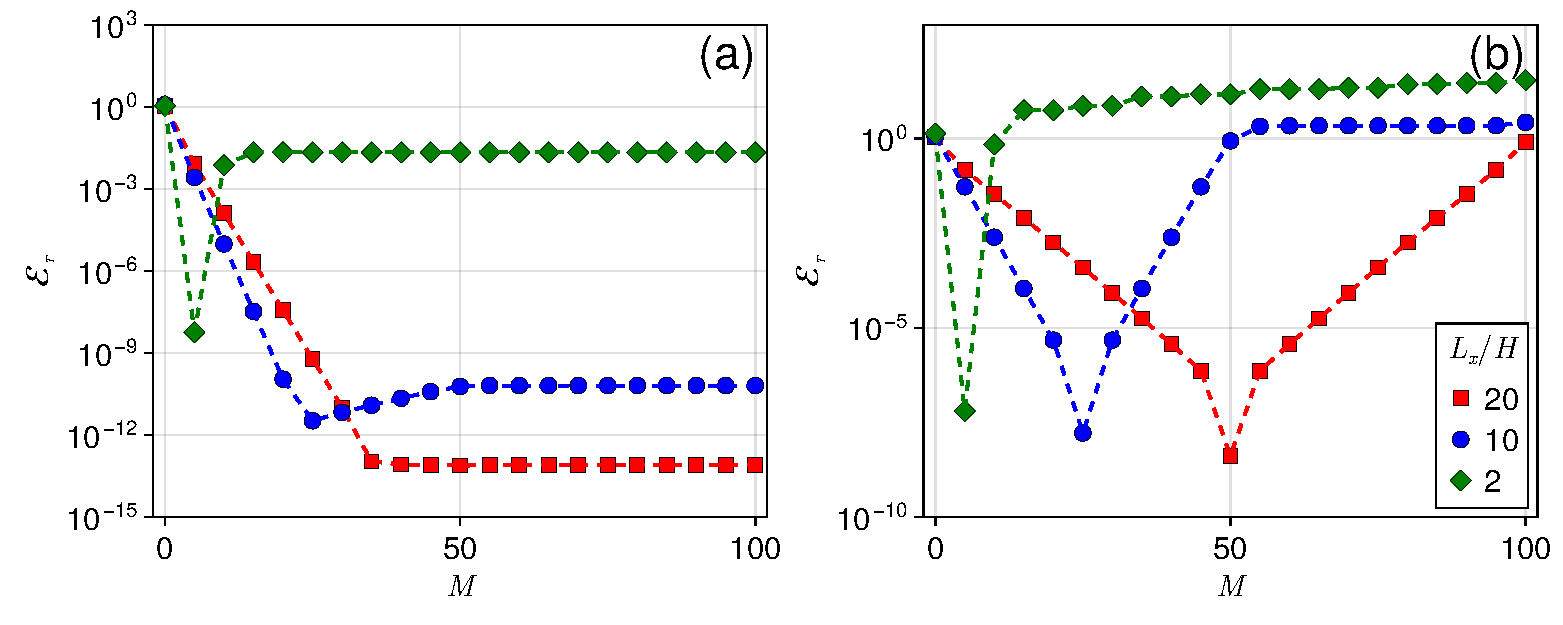
\includegraphics[width=0.98\linewidth]{figs/icm_elc_error_force.pdf}
    \caption{Relative error of force ($\mathcal{E}_r$) in a dielectric-confined Coulomb system with parameters $R = 5$ and $H = 0.5, 1, 5$. In panels (a) and (b), the dielectric contrasts are set to $\gamma_{\T u} = \gamma_{\T d} = \gamma = 0.6$ and $\gamma_{\T u} = \gamma_{\T d} = \gamma = 1$, respectively.}
    \label{fig:icm_elc_error_force}
\end{figure}

\begin{figure}[htbp]
    \centering
    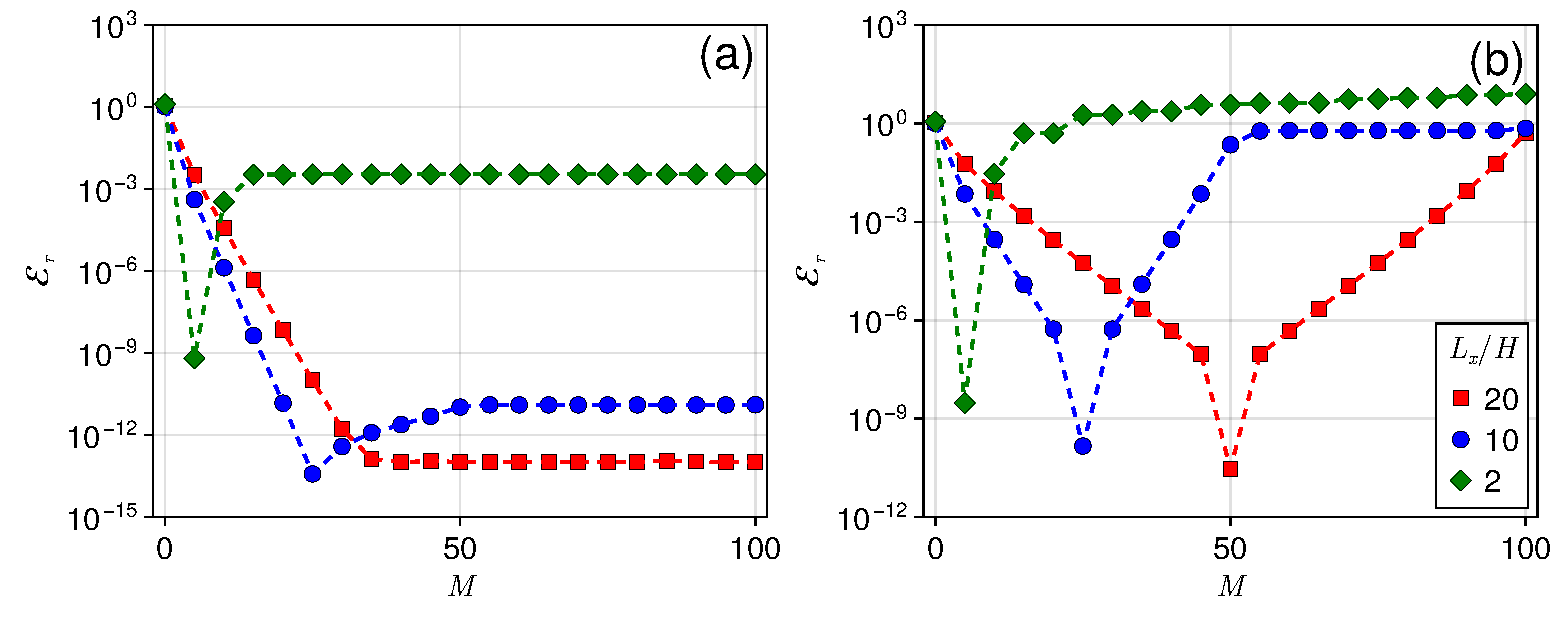
\includegraphics[width=0.98\linewidth]{figs/icm_elc_error.pdf}
    \caption{Relative error of energy in a dielectric-confined Coulomb system with parameters $P = 5$ and $H = 0.5, 1, 5$. In panels (a) and (b), the dielectric contrasts are set to $\gamma_{\T u} = \gamma_{\T d} = \gamma = 0.6$ and $\gamma_{\T u} = \gamma_{\T d} = \gamma = 1$, respectively.}
    \label{fig:icm_elc_error}
\end{figure}

\chapter{Supplementary Results for the Methods}
\label{chp_appendix_soe}
\section{Force expressions of SOEwald2D} \label{app::force}

The Fourier component of force acting on the $i$th particle can be evaluated by taking the gradient of the energy with respect to the particle's position vector $\bm{r}_{i}$,
\begin{equation}\label{eq::Fi}
	\V{F}_{\ell}^i  \approx \V{F}^{i}_{\text{l},\text{SOE}} = -\grad_{\V{r}_{i}} U_{\ell,\text{SOE}} =  -\sum_{\bm{h}\neq \bm{0}} \grad_{\V{r}_{i}}U_{\ell,\text{SOE}}^{\V{h}} -\grad_{\V{r}_{i}} U_{\ell,\text{SOE}}^{\V{0}}
\end{equation}
where
\begin{align}    
	\grad_{\V{r}_{i}}U_{\ell,\text{SOE}}^{\V{h}} &= - \frac{\pi q_{i}}{L_x L_y} \left[ \sum_{1 \leq j < i} q_{j} \grad_{\V{r}_{i}} \varphi_{\text{SOE}}^{\V{h}}(\V{r}_{i}, \V{r}_{j}) +  \sum_{i < j \leq N} q_{j} \grad_{\V{r}_{i}} \varphi_{\text{SOE}}^{\V{h}}(\V{r}_{j}, \V{r}_{i}) \right]\;,\\
	\grad_{\V{r}_{i}} U_{\ell,\text{SOE}}^{\V{0}} &= - \frac{2 \pi q_{i}}{L_x L_y} \left[ \sum_{1 \leq j < i} q_{j} \grad_{\V{r}_{i}} \varphi^{\bm{0}}_{\text{SOE}}(\bm{r}_{i}, \bm{r}_{j}) + \sum_{i < j \leq N} q_{j} \grad_{\V{r}_{i}} \varphi^{\bm{0}}_{\text{SOE}}(\bm{r}_{j}, \bm{r}_{i})\right]\;.
\end{align}
Using the approximation Eqs.~\eqref{eq::SOEphi},~\eqref{eq::dz_plus} and~\eqref{eq::dz_minus}, one can write the derivative in periodic directions as
\begin{equation}
	\begin{split}
		\partial_{\bm{\rho}_{i}} \varphi_{\text{SOE}}^{\V{h}}(\V{r}_{i}, \V{r}_{j}) & = \frac{\m{i} \V{h} e^{ \m{i} \V{h} \cdot \V{\rho}_{ij}}}{h} \left[\xi^{+}_M(h, z_{ij})+\xi^{-}_M(h, z_{ij})\right]\\
		&=\frac{2\alpha e^{-h^2/(4\alpha^2)}}{\sqrt{\pi}h} \m{i} \bm{h}e^{\m{i} \V{h} \cdot \V{\rho}_{ij}} \sum_{\ell = 1}^{M}  \frac{w_l}{\alpha^2 s_l^2 - h^2}\left( 2 \alpha s_l e^{-h z_{ij}} - 2 h e^{-\alpha s_l z_{ij}}\right),
	\end{split}
\end{equation}
and in~$z$ direction as
\begin{equation}\label{eq:z-der}
	\begin{split}
		\partial_{z_{i}} \varphi_{\text{SOE}}^{\V{h}}(\V{r}_{i}, \V{r}_{j}) & = \frac{e^{\m{i} \V{h} \cdot \V{\rho}_{ij}}}{h} \left[\partial_{z_{i}} \xi^{+}_M(h, z_{ij}) + \partial_{z_{i}} \xi^{-}_M(h, z_{ij})\right]\\
		&=\frac{2 \alpha e^{-h^2/(4\alpha^2)}}{\sqrt{\pi}}e^{ \m{i} \V{h} \cdot \V{\rho}_{ij}} \sum_{\ell = 1}^{M}  \frac{w_l}{\alpha^2 s_l^2 - h^2}\left( - 2 \alpha s_l e^{-h z_{ij}} + 2 \alpha s_l e^{- \alpha s_l z_{ij}}\right)\;.
	\end{split}
\end{equation}
The partial derivatives of zero-frequency mode with respect to the periodic directions are zero, and the SOE approximation of its $z$-derivative is given by
\begin{equation}\label{eq:dzphi_0}
	\begin{split}
		\partial_{z_{i}} \varphi^{\bm{0}}_{\text{SOE}}(\bm{r}_{i},\bm{r}_{j}) 
		& = \sum_{l=1}^{M} \frac{w_l}{\sqrt{\pi}} \partial_{z_{i}} \left[\frac{2z_{ij}}{s_l}+\left(\frac{1}{\alpha} - \frac{2z_{ij}}{s_l}\right)e^{-\alpha s_l z_{ij}}\right] \\
		& = \sum_{l=1}^{M} \frac{w_l}{\sqrt{\pi}} \left[ \frac{2}{s_l} - \left( s_l + \frac{2}{s_l} - 2 \alpha z_{ij} \right) e^{-\alpha s_l z_{ij}} \right]\;.
	\end{split}
\end{equation}

It is important to note that the computation of Fourier space forces using Eq.~\eqref{eq::Fi} follows a common recursive procedure with energy, since it has the same structure as given in Eq.~\eqref{eq::33}, and the overall cost for evaluating force on all~$N$ particles for each~$k$ point also amounts to~$O(N)$, and the resulting SOEwald2D method is summarized in Algorithm~\ref{alg:SOEwald2D}.

Moreover, Lemma~\ref{lem::forceerr} establishes the overall error on forces $\bm{F}_{i}$, and the proof follows an almost similar approach to what was done for the energy. %The proof is postponed to~\ref{app::forceerror}

\begin{lem}\label{lem::forceerr}
	The total error of force by the SOEwald2D is given by
	\begin{equation}
		\mathscr{E}_{\bm{F}_{i}} := \mathscr{E}_{\bm{F}_{\emph{s}}^{i}} + \mathscr{E}_{\bm{F}_{\emph{l}}^{i}} + \sum_{\bm{h}\neq \bm{0}} \mathscr{E}_{\bm{F}_{\emph{l}}^i, \emph{SOE}}^{\bm{h}} + \mathscr{E}_{\bm{F}_{\emph{l}}^{i},\emph{SOE}}^{\bm{0}}
	\end{equation}
	where the first two terms are the truncation error and provided in Proposition~\ref{prop::2.12}. The remainder terms 
	\begin{equation}
		\mathscr{E}_{\bm{F}_{\emph{l}}^i,\emph{SOE}}^{\bm{h}} := \bm{F}_{\emph{l}}^{\bm{h}, i} - \bm{F}_{\emph{l},\emph{SOE}}^{\bm{h}, i}, \quad\emph{and} \quad \mathscr{E}_{\bm{F}_{\emph{l}}^{i}, \emph{SOE}}^{\bm{0}} := \bm{F}_{\emph{l}}^{\bm{0}, i}-\bm{F}_{\emph{l}, \emph{SOE}}^{\bm{0}, i}
	\end{equation}
	are the error due to the SOE approximation as Eqs.~\eqref{eq::Fi}-\eqref{eq:z-der}. Given SOE parameters $w_l$ and $s_l$ along with the ideal-gas assumption, one has the following estimate:
	\begin{equation}
		\sum_{\bm{h}\neq\bm{0}} \mathscr{E}_{\bm{F}_{\emph{l}}^i, \emph{SOE}}^{ \bm{h}}\leq \sqrt{2}\lambda_D^2\alpha^2q_{i}^2\varepsilon,\quad\text{and}\quad \mathscr{E}_{\bm{F}_{\emph{l}}^{i},\emph{SOE}}^{\bm{0}}\leq \frac{4\sqrt{\pi}\lambda_D^2 (1+2\alpha)L_z}{L_xL_y}q_{i}^2\varepsilon.
	\end{equation}
\end{lem}



%the electrostatic potential satisfies the Poisson's equation
%\begin{equation}
%-\Delta \phi(\bm{r})=4\pi \rho_{q}(\bm{r}),\quad\rho_{q}(\bm{{r}})=q\rho_+g_{++}(\bm{r})-q\rho_{-}g_{+-}(\bm{r}),
%\end{equation}
%where the charge density are expressed in terms of the charge-charge correlation functions $g_{++}(\bm{r})=g_{--}(\bm{r})(\bm{r})$ and $g_{+-}(\bm{r})=g_{-+}(\bm{r})$, and $\rho_+=\rho_-=\rho/2$ are average densities of positive and negative ions. In the work of Debye and H$\ddot{\text{u}}$ckel, the correlation functions are approximated by $g_{ij}(\bm{r})=e^{-\beta q_j\phi_i(\bm{r})}$, 

%\section{The SOE approximation error of force}\label{app::forceerror}

\section{Force expressions of RBE2D}\label{app::surfacecharge}

In this section, we will discuss the extension of the developed RBE algorithm to handle systems that involve both continuous surface charges and free ions. Without loss of generality, we assume two charged interfaces are located at $z=0$ and $z=H$ and with uniform surface charge density $\sigma_d$ and $\sigma_u$. The system satisfies the charge neutrality condition \begin{equation}\label{eq::chargeneutrality}
    \sum_{i=1}^N q_i+(\sigma_d+\sigma_u)L_xL_y=0\;,
\end{equation}
so that the electrostatic energy and force of the system are both well-defined. When dealing with surface charges, it is common in the literature to handle discrete ions and continuous surface charges separately~\cite{spohr1997effect,yi2017note,yuan2021particle}. The former is typically treated as an infinite summation problem, while the latter is often obtained by solving an additional Poisson equation. %However, during the energy calculation, some divergent terms may arise. Since these terms do not affect the forces, they are often disregarded in a rough manner. 

In this manuscript, we employ a unified methodology where the continuous charge is treated as the limit distribution of an infinite set of discrete charges.
To ensure accuracy, the parameters $M$ and $L_z$ are selected according to the parameter selecting strategy proposed in Section~\ref{sec:parameter}.
As a result, we can accurately describe the force exerted on each mobile ion as:
\begin{equation}
\bm{F}^{\text{c}}(\bm{r}_i)=\bm{F}^{\text{c}}_{\text{real}}(\bm{r}_i)+\bm{F}^{\text{c}}_{\text{Fourier}}(\bm{r}_i)+\bm{F}^{\text{c}}_{\text{wall}}(\bm{r}_i),
\end{equation}
including the real space, the Fourier space, and ion-wall components. The real space component is given by
\begin{equation}\label{eq::F_real_detail}
\begin{split}
\bm{F}_{\text{real}}^{\te{c}}(\bm{r}_i)
& := -q_i\sum_{j=1}^{N} q_j \Biggg[\sum_{\bm{n}}{}^\prime \frac{\left(\bm{r}_{i,\bm{n}} - \bm{r}_{j}\right)}{\abs{\bm{r}_{i,\bm{n}} - \bm{r}_{j}}} K(\abs{\bm{r}_{i,\bm{n}} - \bm{r}_{j}}) \\
&+ \frac{1}{2} \sum_{\bm{n}} \sum_{l=1}^{M} \frac{\gamma_{l}^+\left(\bm{r}_{i,\bm{n}}-\bm{r}_{j+}^{(l)}\right)}{\left|\bm{r}_{i,\bm{n}}-\bm{r}_{j+}^{(l)}\right|} K\left(\left|\bm{r}_{i,\bm{n}}-\bm{r}_{j+}^{(l)}\right|\right)\\
&+\frac{1}{2}\sum_{\bm{n}}\sum_{l=1}^{M}\frac{\gamma_{l}^-\left(\bm{r}_{i,\bm{n}}-\bm{r}_{j-}^{(l)}\right)}{\left|\bm{r}_{i,\bm{n}}-\bm{r}_{j-}^{(l)}\right|}K\left(\left|\bm{r}_{i,\bm{n}}-\bm{r}_{j-}^{(l)}\right|\right)\Biggg]\\
&-\frac{q_i}{2}\sum_{j=1}^{N}q_j\sum_{\bm{n}}\sum_{l=1}^{M}\begin{pmatrix}
1&0&0\\
0&1&0\\
0&0&(-1)^l
\end{pmatrix}\Biggg[
\frac{\gamma_{l}^+\left(\bm{r}_{i,\bm{n}}-\bm{r}_{j+}^{(l)}\right)}{\left|\bm{r}_{i,\bm{n}}-\bm{r}_{j+}^{(l)}\right|}K\left(\left|\bm{r}_{i,\bm{n}}-\bm{r}_{j+}^{(l)}\right|\right)\\
&+\frac{\gamma_{l}^-\left(\bm{r}_{i,\bm{n}}-\bm{r}_{j-}^{(l)}\right)}{\left|\bm{r}_{i,\bm{n}}-\bm{r}_{j-}^{(l)}\right|}K\left(\left|\bm{r}_{i,\bm{n}}-\bm{r}_{j-}^{(l)}\right|\right)\Biggg]
\end{split}
\end{equation}
where $\bm{r}_{i,\bm{n}}=\bm{r}_{i}+\bm{\ell}$, and $K(r):=\text{erfc}(\alpha r)/r^2+2\alpha e^{-\alpha^2r^2}/(\sqrt{\pi}r)$. The Fourier component of force, $\bm{F}^{\text{c}}_{\text{Fourier}}$, has been provided in Eq.~\eqref{eq::52}. In practice, we use the RBE force $\bm{F}^{\text{c},*}_{\text{Fourier}}$ in Eq.~\eqref{eq::important} as an unbiased estimator to $\bm{F}^{\text{c}}_{\text{Fourier}}$, in which the formula of IBC term is more complicated than  {in} the case of  {a} neutral interface:
\begin{equation}\label{eq::IBC}
\begin{split}
\bm{F}_{\text{IBC}}^{M}(\bm{r}_i)=&-\frac{2\pi q_{i}}{L_xL_yL_z}\left[\mathcal{M}_{z}\left(1+\sum_{l=1}^{M}(-1)^{l}\left(\gamma_{+}^{(l)}+\gamma_{-}^{(l)}\right)\right)+\mathcal{M}_{z}^{M}\right]\V{\hat e_z}\\
&+\frac{2\pi q_i}{L_xL_yL_z}\sum_{j=1}^{N}q_j\left[z_i+\sum_{l=1}^{M}(-1)^{l}\left(\gamma_{+}^{(l)}z_{i+}^{(l)}+\gamma_{-}^{(l)}z_{i-}^{(l)}\right)\right]\V{\hat e_z}\\
&+\frac{2\pi q_iz_i}{L_xL_yL_z}\sum_{j=1}^{N}q_j\left[1+\sum_{l=1}^{M}\left(\gamma_{+}^{(l)}+\gamma_{-}^{(l)}\right)\right]\V{\hat e_z},
\end{split}
\end{equation}
where the $z$-direction dipole moments are defined via
\begin{equation}
\mathcal{M}_{z}:=\sum_{i=1}^{N}q_iz_i\quad\text{and}\quad \mathcal{M}_{z}^{M}:=\sum_{i=1}^{N}q_i\left[z_{j}+\sum_{l=1}^{M}\left(\gamma_{+}^{(l)}z_{j+}^{(l)}+\gamma_{-}^{(l)}z_{j-}^{(l)}\right)\right].
\end{equation}
It is important to highlight that if the free ions in the solution continue to fulfill the charge neutrality condition Eq.~\eqref{eq::chargeneutrality}, the last two terms in Eq.~\eqref{eq::IBC} vanish. 
The ion-wall component represents the force exerts on the mobile ions due to the charged walls, and is given by
\begin{equation}
\bm{F}_{\text{wall}}^{\te{c}}:=-2\pi z_{i}q_{i}\left[\sigma_u-\sigma_d+\frac{(\sigma_u+\sigma_d)(\gamma_{\text{top}}-\gamma_{d})\left(1-\gamma_{\text{top}}^{\lceil M/2 \rceil}\gamma_{d}^{\lceil M/2 \rceil}\right)}{1-\gamma_{\text{top}}\gamma_{d}}\right]\V{\hat e_z}.
\end{equation}

\chapter{Supplementary Results for the MD Simulations}
\label{chp_appendix_quasiewald}
\section{Oscillation analyzed via the principal value integral}\label{sec::oscillation}

Here we are trying to explain the oscillatory property of the integral given by
\begin{equation}
    I_o = \int_0^{\infty} \frac{J_0(k \D \rho) \exp{(-k a)}}{\exp{(2H(k_0 - k))} - 1} \text{d}k\;,
\end{equation}
where~$k_0$,~$a$ and~$\rho$ are all positive constants.
The integral can further be divided via Laurent expansion, given by
\begin{equation}
    I_o = \int_0^{\infty} \frac{J_0(k \D \rho) \exp{(-k a)}}{2H(k_0 - k)} \text{d}k + \int_0^{\infty} J_0(k \D \rho) \exp{(-k a)} E(k) \text{d}k\;,
\end{equation}
where~$1/2H(k_0 - k)$ is the leading order term of the Laurent series of~$\frac{1}{e^{2H(k_0 - k)} - 1}$, and~$E(k)$ is the Padé approximant of the rest part, which is a non-divergent smooth function.
Due to the fast decay property of~$\exp{(-k a)}$, the second part leads to a non-oscillatory small contribution to the result, and the oscillation is contributed by the leading order term.

To calculate the integral, we treat it as a function of~$a$, given by
\begin{equation}
    I_{o1}(a) = \int_0^{\infty} \frac{J_0(k \D \rho) \exp{(-k a)}}{2H(k_0 - k)} \text{d}k\;,
\end{equation}
so that we have
\begin{equation}
    \begin{split}
    I_{o1}^{\prime}(a) & = - k I_{o1}(a) = \frac{1}{2H} \int_0^{\infty} J_0(k \D \rho) \exp{(-k a)} \text{d}k - k_0 I_{o1}(a) \\
    & = \frac{1}{2H \sqrt{\D \rho^2 + a^2}} - k_0 I_{o1}(a) \;,
    \end{split}
\end{equation}
which forms a differential equation given by
\begin{equation}
    I_{o1}^{\prime}(a) + k_0 I_{o1}(a) = \frac{1}{2H \sqrt{\D \rho^2 + a^2}}\;.
\end{equation}
Using the general solution of ODE, we have
\begin{equation}
    I_{o1}(a) = \exp{(-k_0 a)} \left[C_1 + \int \frac{\exp{(k_0 a)}}{2H \sqrt{\D \rho^2 + a^2}} \text{d}a \right] = \exp{(-k_0 a)} \left[C_1 + C_2(\rho, k_0, a) \right] \;.
\end{equation}
Notice that
\begin{equation}
    I_{o1}(0) = C_1 + C_2(\D \rho, k_0, 0)\;,
\end{equation}
so that
\begin{equation}
    I_{o1}(a) = \exp{(-k_0 a)} \left[ I_1(0) - C_2(\D \rho, k_0, 0) + C_2(\D \rho, k_0, a) \right]\;.
\end{equation}
Although here we do not know the exact result of integral~$C_2$, its contribution to~$I_{o1}$ is clearly non-oscillatory.
Then we can focus on the first term, which contribute the oscillation, given by 
\begin{equation}
    I_{o2} = \frac{\exp{(-k_0 a)}}{2H} \int_0^{\infty} \frac{J_0(k \D \rho)}{(k_0 - k)} \text{d}k = \frac{\exp{(-k_0 a)}}{2H} \int_0^{\infty} \frac{J_0(k^\prime)}{k_0 \D \rho - k^\prime} \text{d}k^\prime\;,
\end{equation}
so that 
\begin{equation}
    I_o = \frac{\exp{(-k_0 a)}}{2H} \int_0^{\infty} \frac{J_0(k^\prime)}{k_0 \D \rho - k^\prime} \text{d}k^\prime + f(k_0, \D \rho, a)\;.
\end{equation}
where~$f(k_0, \D \rho, a)$ is a non-oscillatory function defined by
\begin{equation}
    \begin{split}
        f(k_0, \D \rho, a) = & \exp{(-k_0 a)} \left[ - C_2(\D \rho, k_0, 0) + C_2(\D \rho, k_0, a) \right] \\
        & + \int_0^{\infty} J_0(k \D \rho) \exp{(-k a)} E(k) \text{d}k
    \end{split}
\end{equation}
Here we define
\begin{equation}
    I_{m} = \int_0^{\infty} \frac{J_0(k^\prime)}{k_0 \D \rho - k^\prime} \text{d}k^\prime\;,
\end{equation}
which is only related to~$k_0 \D \rho$, and the numerical result shows that distance between ~$I_{m}$ converge rapidly to~$\pi$, as shown in Fig.~\ref{fig:I_3}.

\begin{figure}[htbp]
\centering
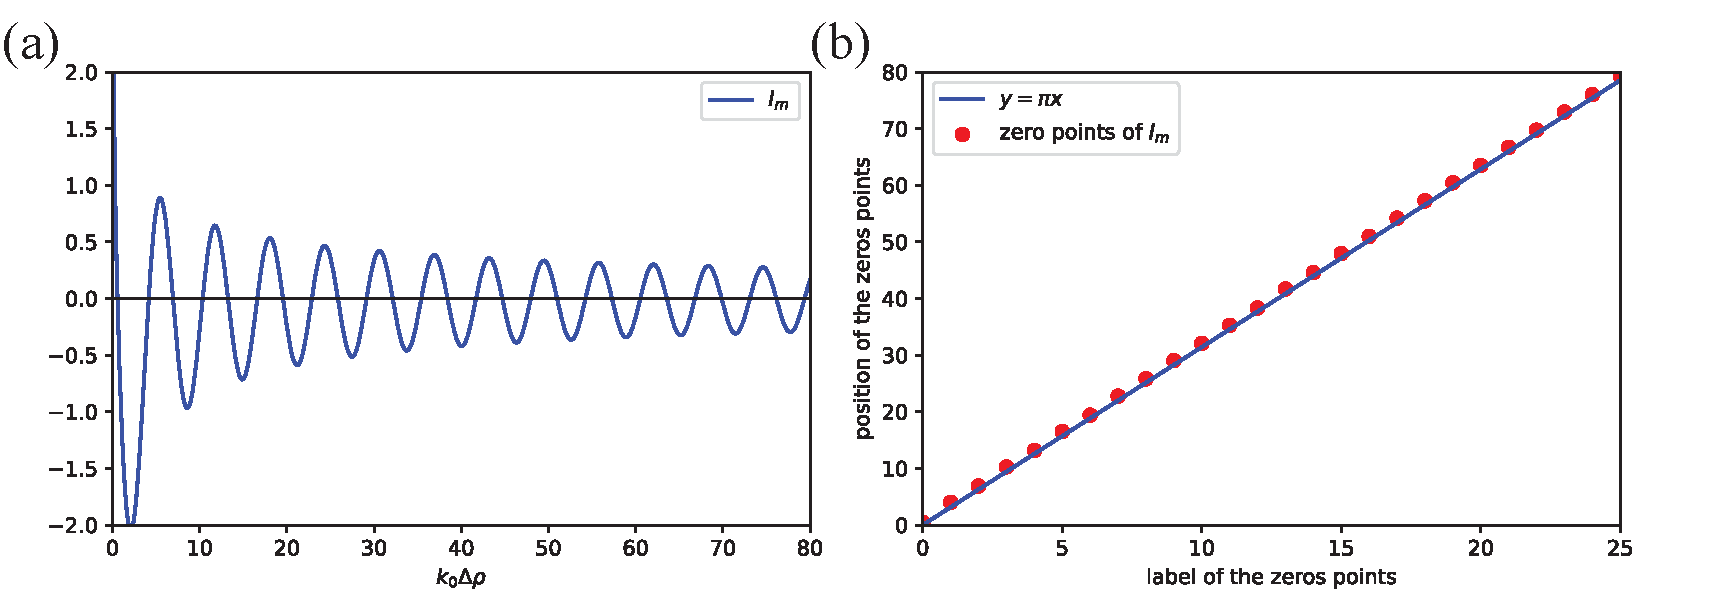
\includegraphics[width=  \linewidth]{figs/I_3.pdf}
\caption{
    Numerical results of~$I_{m}$ is shown in (a), and the position of the zero points are shown in (b).
}
\label{fig:I_3}
\end{figure}


\section{Simulation details}

In the main text, we have shown that the charge oscillation can lead to lattice-like structure formation in dielectric confined quasi-2D systems, and mainly focused on the tunable lattice parameter.
Here we will discuss more about our results.

\begin{figure}[ht]
    \centering
    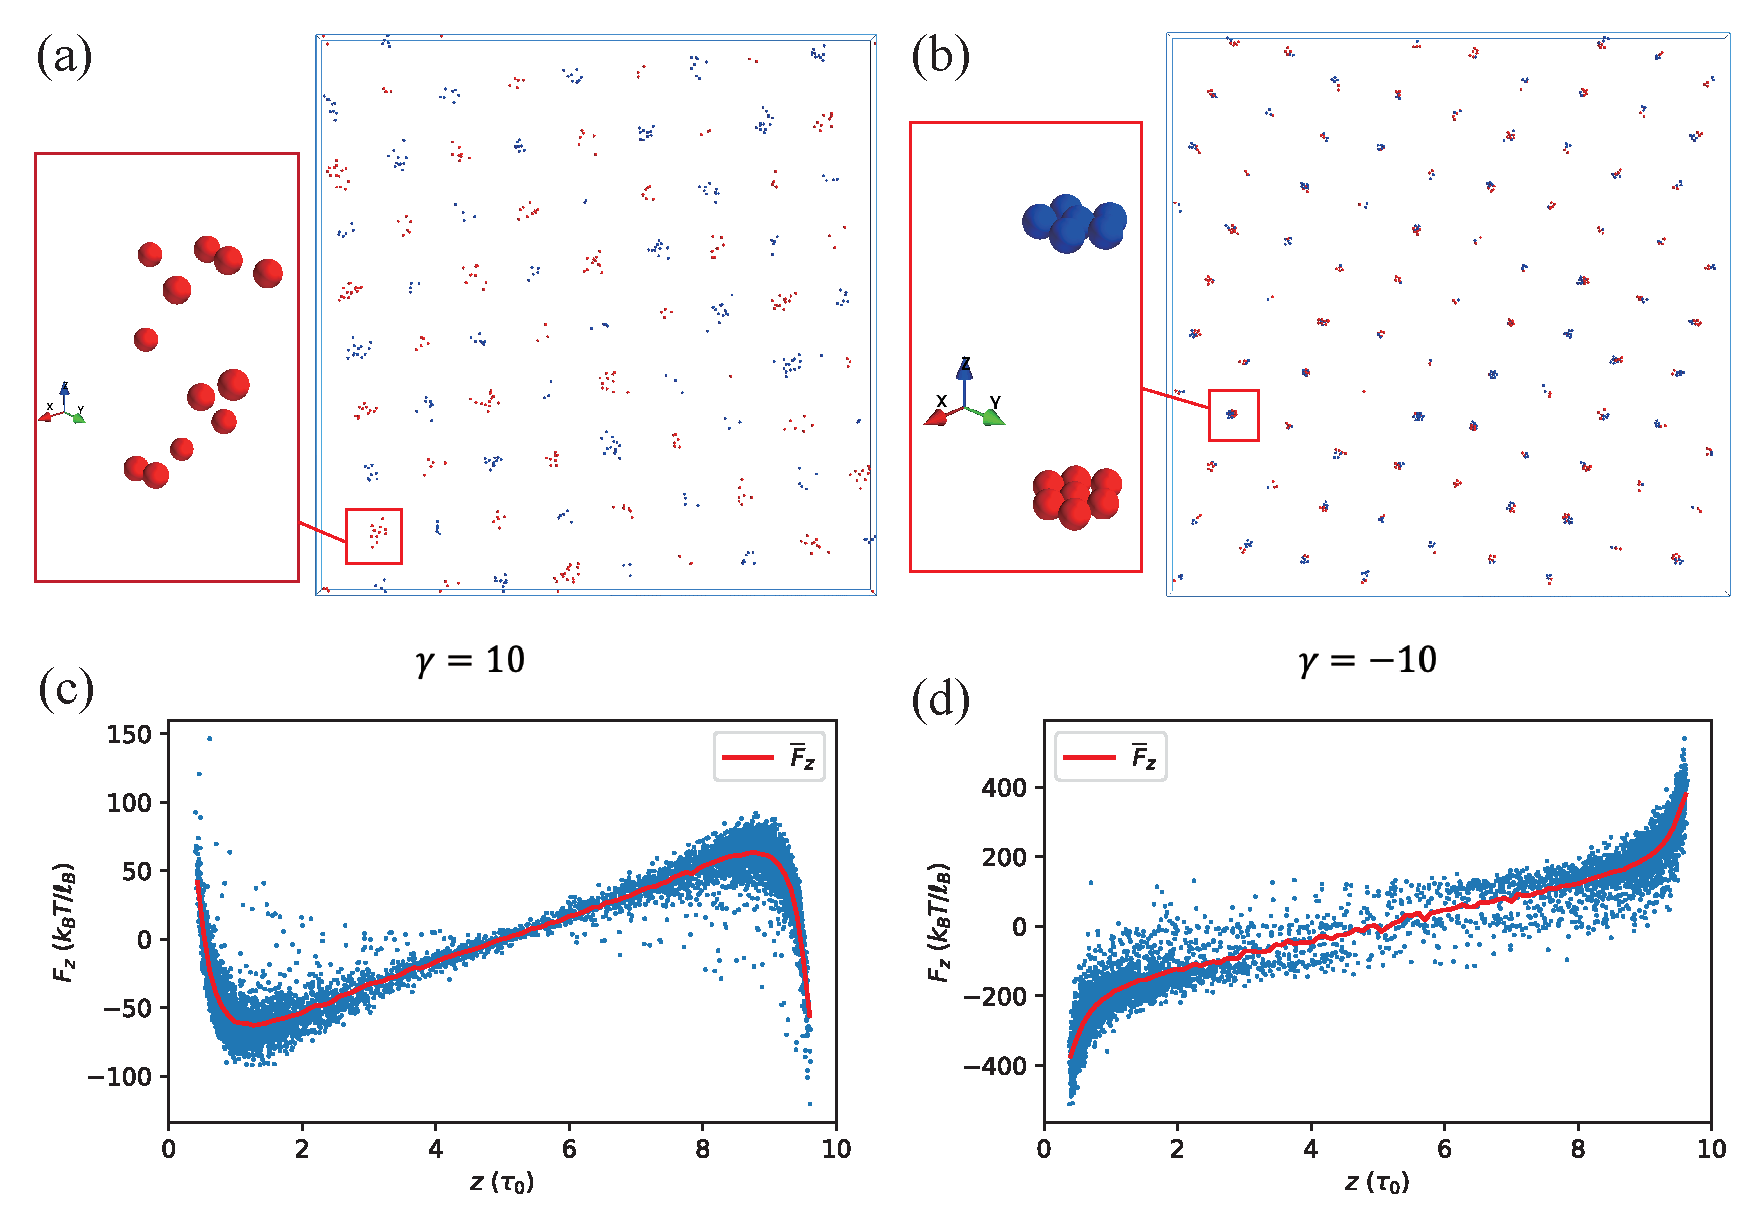
\includegraphics[width = \linewidth]{figs/MD_ball.pdf}
    \caption{The lattice-like structure and the cluster for~$\gamma = \pm 10$ cases are shown in (a) and (b), respectively. Force in~$z$ direction on particles at different position are shown in (b).}
    \label{fig:balls}
\end{figure}

The MD results for the systems which contain~$600$ particles is shown in Fig.~\ref{fig:balls} (a) and (b), and the related videos are given as video1 and video2.
For both simulations, it costs $2 \times 10^6$ time steps in total, and each step takes~$\Delta t = 0.005 t_0$, where~$t_0 = \tau_0 \sqrt{\frac{m_0}{k_B T}}$ is the reduced time scale.
The first $1.5\times 10^6$ steps are performed using the simulated annealing technique to avoid trapping in a metastable state. We start with $T_r=10$ and slowly cooling down the system until it reaches equilibrium at $T_r=1$, after which we continue the simulation for $5 \times 10^5$ time steps for sampling.

The ions distribute near the substrates and pair with other ions on the opposite side.
For~$\gamma = 10$ and~$-10$ cases, the pairs are symmetric and anti-symmetric, respectively, as shown in the sub-figure.
The difference come from the sign of the reflection rate, which determines whether the polarized charges at opposite positions are of the same sign or of different sign, thus determines the symmetry of the ions on the opposite sites.

Shapes of the clusters are also different.
For both cases, we attribute the cluster formation to the strong polarization charge with different sign on the substrate as shown in Fig.~1~(a) of the main text, which form a deep potential well and trapped these ions inside.
In the transverse direction, when~$\gamma = 10$, the ions forms ion liquid and separate from each other, and when~$\gamma = -10$, the ions are closely packed, because of the force in transverse direction between ions with the same sign are repulsive or attractive at short range, respectively.
In the vertical direction, we calculated forces in~$z$ to explain the distributions obtained, as shown in Fig.~\ref{fig:balls} (c) and (d).
When~$\gamma = 10$, we found that the surface with opposite sign reverse the force in the middle region and pull the ions to the substrates, so that the ions are distributed near the substrates but not closely touching.
When~$\gamma = -10$, the force is purely attractive and the ions are all closely attached to the substrates.

%%%%%%%%%%%%%%%%%%%%%%%%%%%%%%%%%%%%%%%%%%%%%%%%%%%%%%%%%%%%%%%%%%%%%%%%%
%                                                                       %
%     11) BIOGRAPHY (optional)                                          %
%                                                                       %
% \biography and \endbiography are used to define the optional          %
% Biography of the author of the Thesis.                                %
%                                                                       %
%%%%%%%%%%%%%%%%%%%%%%%%%%%%%%%%%%%%%%%%%%%%%%%%%%%%%%%%%%%%%%%%%%%%%%%%%

\end{document}
